\documentclass{book}
\usepackage[a4paper,top=2.5cm,bottom=2.5cm,left=2.5cm,right=2.5cm]{geometry}
\usepackage{makeidx}
\usepackage{natbib}
\usepackage{graphicx}
\usepackage{multicol}
\usepackage{float}
\usepackage{listings}
\usepackage{color}
\usepackage{ifthen}
\usepackage[table]{xcolor}
\usepackage{textcomp}
\usepackage{alltt}
\usepackage{ifpdf}
\ifpdf
\usepackage[pdftex,
            pagebackref=true,
            colorlinks=true,
            linkcolor=blue,
            unicode
           ]{hyperref}
\else
\usepackage[ps2pdf,
            pagebackref=true,
            colorlinks=true,
            linkcolor=blue,
            unicode
           ]{hyperref}
\usepackage{pspicture}
\fi
\usepackage[utf8]{inputenc}
\usepackage{mathptmx}
\usepackage[scaled=.90]{helvet}
\usepackage{courier}
\usepackage{sectsty}
\usepackage[titles]{tocloft}
\usepackage{doxygen}
\lstset{language=C++,inputencoding=utf8,basicstyle=\footnotesize,breaklines=true,breakatwhitespace=true,tabsize=4,numbers=left }
\makeindex
\setcounter{tocdepth}{3}
\renewcommand{\footrulewidth}{0.4pt}
\renewcommand{\familydefault}{\sfdefault}
\hfuzz=15pt
\setlength{\emergencystretch}{15pt}
\hbadness=750
\tolerance=750
\begin{document}
\hypersetup{pageanchor=false,citecolor=blue}
\begin{titlepage}
\vspace*{7cm}
\begin{center}
{\Large P\-B Analytical \\[1ex]\large V1 }\\
\vspace*{1cm}
{\large Generated by Doxygen 1.8.1}\\
\vspace*{0.5cm}
{\small Wed Jul 2 2014 13:47:00}\\
\end{center}
\end{titlepage}
\clearemptydoublepage
\pagenumbering{roman}
\tableofcontents
\clearemptydoublepage
\pagenumbering{arabic}
\hypersetup{pageanchor=true,citecolor=blue}
\chapter{Class Index}
\section{Class Hierarchy}
This inheritance list is sorted roughly, but not completely, alphabetically\-:\begin{DoxyCompactList}
\item \contentsline{section}{A\-A}{\pageref{classAA}}{}
\item \contentsline{section}{C\-Atom}{\pageref{classCAtom}}{}
\item \contentsline{section}{C\-B\-D}{\pageref{classCBD}}{}
\item \contentsline{section}{C\-M\-Coeff}{\pageref{classCMCoeff}}{}
\begin{DoxyCompactList}
\item \contentsline{section}{C\-S\-H\-Coeff}{\pageref{classCSHCoeff}}{}
\end{DoxyCompactList}
\item \contentsline{section}{C\-M\-P\-E}{\pageref{classCMPE}}{}
\item \contentsline{section}{C\-O\-N\-T\-A\-C\-T}{\pageref{structCONTACT}}{}
\item \contentsline{section}{C\-P\-D\-B}{\pageref{classCPDB}}{}
\item \contentsline{section}{C\-Pnt}{\pageref{classCPnt}}{}
\item \contentsline{section}{C\-Protein}{\pageref{classCProtein}}{}
\item \contentsline{section}{C\-Quat}{\pageref{classCQuat}}{}
\item \contentsline{section}{C\-Rot\-Coeff}{\pageref{classCRotCoeff}}{}
\item \contentsline{section}{C\-Sp\-Pnt}{\pageref{classCSpPnt}}{}
\item \contentsline{section}{C\-Trans\-Coeff}{\pageref{classCTransCoeff}}{}
\item \contentsline{section}{C\-Tri\-Coeff}{\pageref{classCTriCoeff}}{}
\begin{DoxyCompactList}
\item \contentsline{section}{C\-Grad\-Coeff}{\pageref{classCGradCoeff}}{}
\item \contentsline{section}{C\-Torq\-Coeff}{\pageref{classCTorqCoeff}}{}
\end{DoxyCompactList}
\item \contentsline{section}{C\-X\-Form}{\pageref{classCXForm}}{}
\end{DoxyCompactList}

\chapter{Class Index}
\section{Class List}
Here are the classes, structs, unions and interfaces with brief descriptions\-:\begin{DoxyCompactList}
\item\contentsline{section}{\hyperlink{classAA}{A\-A} }{\pageref{classAA}}{}
\item\contentsline{section}{\hyperlink{classCAtom}{C\-Atom} }{\pageref{classCAtom}}{}
\item\contentsline{section}{\hyperlink{classCBD}{C\-B\-D} }{\pageref{classCBD}}{}
\item\contentsline{section}{\hyperlink{classCGradCoeff}{C\-Grad\-Coeff} }{\pageref{classCGradCoeff}}{}
\item\contentsline{section}{\hyperlink{classCMCoeff}{C\-M\-Coeff} }{\pageref{classCMCoeff}}{}
\item\contentsline{section}{\hyperlink{classCMPE}{C\-M\-P\-E} }{\pageref{classCMPE}}{}
\item\contentsline{section}{\hyperlink{structCONTACT}{C\-O\-N\-T\-A\-C\-T} }{\pageref{structCONTACT}}{}
\item\contentsline{section}{\hyperlink{classCPDB}{C\-P\-D\-B} }{\pageref{classCPDB}}{}
\item\contentsline{section}{\hyperlink{classCPnt}{C\-Pnt} }{\pageref{classCPnt}}{}
\item\contentsline{section}{\hyperlink{classCProtein}{C\-Protein} }{\pageref{classCProtein}}{}
\item\contentsline{section}{\hyperlink{classCQuat}{C\-Quat} }{\pageref{classCQuat}}{}
\item\contentsline{section}{\hyperlink{classCRotCoeff}{C\-Rot\-Coeff} }{\pageref{classCRotCoeff}}{}
\item\contentsline{section}{\hyperlink{classCSHCoeff}{C\-S\-H\-Coeff} }{\pageref{classCSHCoeff}}{}
\item\contentsline{section}{\hyperlink{classCSpPnt}{C\-Sp\-Pnt} }{\pageref{classCSpPnt}}{}
\item\contentsline{section}{\hyperlink{classCTorqCoeff}{C\-Torq\-Coeff} }{\pageref{classCTorqCoeff}}{}
\item\contentsline{section}{\hyperlink{classCTransCoeff}{C\-Trans\-Coeff} }{\pageref{classCTransCoeff}}{}
\item\contentsline{section}{\hyperlink{classCTriCoeff}{C\-Tri\-Coeff} }{\pageref{classCTriCoeff}}{}
\item\contentsline{section}{\hyperlink{classCXForm}{C\-X\-Form} }{\pageref{classCXForm}}{}
\end{DoxyCompactList}

\chapter{File Index}
\section{File List}
Here is a list of all files with brief descriptions\-:\begin{DoxyCompactList}
\item\contentsline{section}{\hyperlink{BD_8cpp}{B\-D.\-cpp} }{\pageref{BD_8cpp}}{}
\item\contentsline{section}{\hyperlink{BD_8h}{B\-D.\-h} }{\pageref{BD_8h}}{}
\item\contentsline{section}{\hyperlink{gradcoeff_8cpp}{gradcoeff.\-cpp} }{\pageref{gradcoeff_8cpp}}{}
\item\contentsline{section}{\hyperlink{gradcoeff_8h}{gradcoeff.\-h} }{\pageref{gradcoeff_8h}}{}
\item\contentsline{section}{\hyperlink{mcoeff_8cpp}{mcoeff.\-cpp} }{\pageref{mcoeff_8cpp}}{}
\item\contentsline{section}{\hyperlink{mcoeff_8h}{mcoeff.\-h} }{\pageref{mcoeff_8h}}{}
\item\contentsline{section}{\hyperlink{mpe_8cpp}{mpe.\-cpp} }{\pageref{mpe_8cpp}}{}
\item\contentsline{section}{\hyperlink{mpe_8h}{mpe.\-h} }{\pageref{mpe_8h}}{}
\item\contentsline{section}{\hyperlink{pdb_8cpp}{pdb.\-cpp} }{\pageref{pdb_8cpp}}{}
\item\contentsline{section}{\hyperlink{pdb_8h}{pdb.\-h} }{\pageref{pdb_8h}}{}
\item\contentsline{section}{\hyperlink{protein_8cpp}{protein.\-cpp} }{\pageref{protein_8cpp}}{}
\item\contentsline{section}{\hyperlink{protein_8h}{protein.\-h} }{\pageref{protein_8h}}{}
\item\contentsline{section}{\hyperlink{rotcoeff_8cpp}{rotcoeff.\-cpp} }{\pageref{rotcoeff_8cpp}}{}
\item\contentsline{section}{\hyperlink{rotcoeff_8h}{rotcoeff.\-h} }{\pageref{rotcoeff_8h}}{}
\item\contentsline{section}{\hyperlink{shcoeff_8cpp}{shcoeff.\-cpp} }{\pageref{shcoeff_8cpp}}{}
\item\contentsline{section}{\hyperlink{shcoeff_8h}{shcoeff.\-h} }{\pageref{shcoeff_8h}}{}
\item\contentsline{section}{\hyperlink{torqcoeff_8cpp}{torqcoeff.\-cpp} }{\pageref{torqcoeff_8cpp}}{}
\item\contentsline{section}{\hyperlink{torqcoeff_8h}{torqcoeff.\-h} }{\pageref{torqcoeff_8h}}{}
\item\contentsline{section}{\hyperlink{transcoeff_8cpp}{transcoeff.\-cpp} }{\pageref{transcoeff_8cpp}}{}
\item\contentsline{section}{\hyperlink{transcoeff_8h}{transcoeff.\-h} }{\pageref{transcoeff_8h}}{}
\item\contentsline{section}{\hyperlink{tricoeff_8cpp}{tricoeff.\-cpp} }{\pageref{tricoeff_8cpp}}{}
\item\contentsline{section}{\hyperlink{tricoeff_8h}{tricoeff.\-h} }{\pageref{tricoeff_8h}}{}
\item\contentsline{section}{\hyperlink{util_8h}{util.\-h} }{\pageref{util_8h}}{}
\item\contentsline{section}{\hyperlink{xform_8cpp}{xform.\-cpp} }{\pageref{xform_8cpp}}{}
\item\contentsline{section}{\hyperlink{xform_8h}{xform.\-h} }{\pageref{xform_8h}}{}
\end{DoxyCompactList}

\chapter{Class Documentation}
\hypertarget{classAA}{\section{A\-A Class Reference}
\label{classAA}\index{A\-A@{A\-A}}
}


The \hyperlink{classAA}{A\-A} class.  




{\ttfamily \#include $<$pdb.\-h$>$}

\subsection*{Public Types}
\begin{DoxyCompactItemize}
\item 
enum \hyperlink{classAA_a8717db02e7eeaac316898736843fa600}{A\-A\-C\-O\-D\-E} \{ \\*
\hyperlink{classAA_a8717db02e7eeaac316898736843fa600a17332f1fda1d77630ce34d02a1f68e5d}{A\-L\-A}, 
\hyperlink{classAA_a8717db02e7eeaac316898736843fa600aca714992a8e9579da27a0fbf9d48a5fd}{A\-R\-G}, 
\hyperlink{classAA_a8717db02e7eeaac316898736843fa600a52af7e75fa5f9f289b5f6fc1910a431d}{A\-S\-N}, 
\hyperlink{classAA_a8717db02e7eeaac316898736843fa600aafe8caeae4990f1af233fa5f7e5c15cf}{A\-S\-P}, 
\\*
\hyperlink{classAA_a8717db02e7eeaac316898736843fa600a1aa30f6957e958e3a598e22290dd9aaf}{C\-Y\-S}, 
\hyperlink{classAA_a8717db02e7eeaac316898736843fa600a48ebbfb21d749d2fc8173e9911375f76}{G\-L\-N}, 
\hyperlink{classAA_a8717db02e7eeaac316898736843fa600a364c2f447e99c0351f7a47350f4c1a21}{G\-L\-U}, 
\hyperlink{classAA_a8717db02e7eeaac316898736843fa600a6d39f32ab6ef641a052e7a945c93183c}{G\-L\-Y}, 
\\*
\hyperlink{classAA_a8717db02e7eeaac316898736843fa600aaf01c20386a10cb2ea5dbbdbca7b583f}{H\-I\-S}, 
\hyperlink{classAA_a8717db02e7eeaac316898736843fa600a8700eb27f767befe2837e19d5efc4cd9}{I\-L\-E}, 
\hyperlink{classAA_a8717db02e7eeaac316898736843fa600a2de4c58cee86c85529491465dfa2a6af}{L\-E\-U}, 
\hyperlink{classAA_a8717db02e7eeaac316898736843fa600a7972b64ba1692406dffb174361ba3e2c}{L\-Y\-S}, 
\\*
\hyperlink{classAA_a8717db02e7eeaac316898736843fa600a29cdb3d97ce13d9ed497dda69188cd30}{M\-E\-T}, 
\hyperlink{classAA_a8717db02e7eeaac316898736843fa600ab61eea814f02c0bfb8ad583be990c0b7}{P\-H\-E}, 
\hyperlink{classAA_a8717db02e7eeaac316898736843fa600a8a897d9c18f7c8a75e0fd17743602fc8}{P\-R\-O}, 
\hyperlink{classAA_a8717db02e7eeaac316898736843fa600ae00b524e87bde55b1e65124e91c22e9e}{S\-E\-R}, 
\\*
\hyperlink{classAA_a8717db02e7eeaac316898736843fa600ad7c137e98cba8533a976dc060ed47580}{T\-H\-R}, 
\hyperlink{classAA_a8717db02e7eeaac316898736843fa600a80f39d69089385967584e0d860abf8c8}{T\-R\-P}, 
\hyperlink{classAA_a8717db02e7eeaac316898736843fa600a14daa08339ebd75d5856d9e99325a7eb}{T\-Y\-R}, 
\hyperlink{classAA_a8717db02e7eeaac316898736843fa600ac22cf3896ad17e3136d9ed2f403e31f9}{V\-A\-L}, 
\\*
\hyperlink{classAA_a8717db02e7eeaac316898736843fa600a2362193b9e548fbc61b1b502e539f176}{N\-T\-R}, 
\hyperlink{classAA_a8717db02e7eeaac316898736843fa600a67989ca37e3ee8b892f7569ca60a9bbd}{C\-T\-R}
 \}
\begin{DoxyCompactList}\small\item\em The \hyperlink{classAA}{A\-A} class enum A\-A\-C\-O\-D\-E. \end{DoxyCompactList}\end{DoxyCompactItemize}
\subsection*{Public Member Functions}
\begin{DoxyCompactItemize}
\item 
const \hyperlink{classCAtom}{C\-Atom} $\ast$ \hyperlink{classAA_aa271a8269c3a69c795651b87768abd3c}{operator\mbox{[}$\,$\mbox{]}} (const char $\ast$aname) const 
\begin{DoxyCompactList}\small\item\em The \hyperlink{classAA}{A\-A} \mbox{[}\mbox{]} operator. \end{DoxyCompactList}\item 
const \hyperlink{classCAtom}{C\-Atom} \& \hyperlink{classAA_ad47e1014c42578100eb951d057130d60}{operator\mbox{[}$\,$\mbox{]}} (int i) const 
\begin{DoxyCompactList}\small\item\em The \hyperlink{classAA}{A\-A} \mbox{[}\mbox{]} operator. \end{DoxyCompactList}\item 
\hyperlink{classAA_a8717db02e7eeaac316898736843fa600}{A\-A\-C\-O\-D\-E} \hyperlink{classAA_a7bb2b102b435f41fa3c78c1cded8ce93}{get\-Type} () const 
\item 
int \hyperlink{classAA_a296b621ecb2dc785e0c27614dab7df37}{get\-Num\-Atoms} () const 
\item 
void \hyperlink{classAA_a111b14b73321f7fbd0e910fe7377d3e2}{set\-Type} (\hyperlink{classAA_a8717db02e7eeaac316898736843fa600}{A\-A\-C\-O\-D\-E} type)
\item 
void \hyperlink{classAA_ae0851c13f0b0aee431c4b90a17a58c7a}{insert\-Atom} (\hyperlink{classCAtom}{C\-Atom} \&atom)
\item 
void \hyperlink{classAA_a77290c917ac630708465bb700c9a1d91}{clear} ()
\end{DoxyCompactItemize}
\subsection*{Static Public Member Functions}
\begin{DoxyCompactItemize}
\item 
static \hyperlink{classAA_a8717db02e7eeaac316898736843fa600}{A\-A\-C\-O\-D\-E} \hyperlink{classAA_a4586e72f7a09f932e29188a5098f124f}{get\-A\-A\-Code} (const char $\ast$aa)
\begin{DoxyCompactList}\small\item\em The \hyperlink{classAA}{A\-A} class function get\-A\-A\-Code. \end{DoxyCompactList}\item 
static const char $\ast$ \hyperlink{classAA_a1ae2a562a71d05aa8c1f9b3c7136e3b7}{get\-Name} (\hyperlink{classAA_a8717db02e7eeaac316898736843fa600}{A\-A\-C\-O\-D\-E} code)
\end{DoxyCompactItemize}
\subsection*{Static Public Attributes}
\begin{DoxyCompactItemize}
\item 
static const char \hyperlink{classAA_a979027b32adbcc9f5eabeaf580d243b6}{A\-A\-N\-A\-M\-E} \mbox{[}\hyperlink{pdb_8h_aaa82008f92b935630ccf49c27a4bcc6e}{N\-U\-M\-\_\-\-A\-A\-S}\mbox{]}\mbox{[}4\mbox{]}
\begin{DoxyCompactList}\small\item\em 3 Letter codes for each amino acid \end{DoxyCompactList}\item 
static const char \hyperlink{classAA_ad31fab7fcd16661c068535ca46524a6a}{A\-A\-L\-E\-T\-T\-E\-R} \mbox{[}\hyperlink{pdb_8h_aaa82008f92b935630ccf49c27a4bcc6e}{N\-U\-M\-\_\-\-A\-A\-S}\mbox{]}\mbox{[}2\mbox{]}
\begin{DoxyCompactList}\small\item\em 1 Letter codes for each amino acid \end{DoxyCompactList}\end{DoxyCompactItemize}


\subsection{Detailed Description}
The \hyperlink{classAA}{A\-A} class. 

The class that contains all details for an amino acid object 

\subsection{Member Enumeration Documentation}
\hypertarget{classAA_a8717db02e7eeaac316898736843fa600}{\index{A\-A@{A\-A}!A\-A\-C\-O\-D\-E@{A\-A\-C\-O\-D\-E}}
\index{A\-A\-C\-O\-D\-E@{A\-A\-C\-O\-D\-E}!AA@{A\-A}}
\subsubsection[{A\-A\-C\-O\-D\-E}]{\setlength{\rightskip}{0pt plus 5cm}enum {\bf A\-A\-::\-A\-A\-C\-O\-D\-E}}}\label{classAA_a8717db02e7eeaac316898736843fa600}


The \hyperlink{classAA}{A\-A} class enum A\-A\-C\-O\-D\-E. 

An enumerator for the amino acids given by their 3 letter codes \begin{Desc}
\item[Enumerator\-: ]\par
\begin{description}
\index{A\-L\-A@{A\-L\-A}!A\-A@{A\-A}}\index{A\-A@{A\-A}!A\-L\-A@{A\-L\-A}}\item[{\em 
\hypertarget{classAA_a8717db02e7eeaac316898736843fa600a17332f1fda1d77630ce34d02a1f68e5d}{A\-L\-A}\label{classAA_a8717db02e7eeaac316898736843fa600a17332f1fda1d77630ce34d02a1f68e5d}
}]\index{A\-R\-G@{A\-R\-G}!A\-A@{A\-A}}\index{A\-A@{A\-A}!A\-R\-G@{A\-R\-G}}\item[{\em 
\hypertarget{classAA_a8717db02e7eeaac316898736843fa600aca714992a8e9579da27a0fbf9d48a5fd}{A\-R\-G}\label{classAA_a8717db02e7eeaac316898736843fa600aca714992a8e9579da27a0fbf9d48a5fd}
}]\index{A\-S\-N@{A\-S\-N}!A\-A@{A\-A}}\index{A\-A@{A\-A}!A\-S\-N@{A\-S\-N}}\item[{\em 
\hypertarget{classAA_a8717db02e7eeaac316898736843fa600a52af7e75fa5f9f289b5f6fc1910a431d}{A\-S\-N}\label{classAA_a8717db02e7eeaac316898736843fa600a52af7e75fa5f9f289b5f6fc1910a431d}
}]\index{A\-S\-P@{A\-S\-P}!A\-A@{A\-A}}\index{A\-A@{A\-A}!A\-S\-P@{A\-S\-P}}\item[{\em 
\hypertarget{classAA_a8717db02e7eeaac316898736843fa600aafe8caeae4990f1af233fa5f7e5c15cf}{A\-S\-P}\label{classAA_a8717db02e7eeaac316898736843fa600aafe8caeae4990f1af233fa5f7e5c15cf}
}]\index{C\-Y\-S@{C\-Y\-S}!A\-A@{A\-A}}\index{A\-A@{A\-A}!C\-Y\-S@{C\-Y\-S}}\item[{\em 
\hypertarget{classAA_a8717db02e7eeaac316898736843fa600a1aa30f6957e958e3a598e22290dd9aaf}{C\-Y\-S}\label{classAA_a8717db02e7eeaac316898736843fa600a1aa30f6957e958e3a598e22290dd9aaf}
}]\index{G\-L\-N@{G\-L\-N}!A\-A@{A\-A}}\index{A\-A@{A\-A}!G\-L\-N@{G\-L\-N}}\item[{\em 
\hypertarget{classAA_a8717db02e7eeaac316898736843fa600a48ebbfb21d749d2fc8173e9911375f76}{G\-L\-N}\label{classAA_a8717db02e7eeaac316898736843fa600a48ebbfb21d749d2fc8173e9911375f76}
}]\index{G\-L\-U@{G\-L\-U}!A\-A@{A\-A}}\index{A\-A@{A\-A}!G\-L\-U@{G\-L\-U}}\item[{\em 
\hypertarget{classAA_a8717db02e7eeaac316898736843fa600a364c2f447e99c0351f7a47350f4c1a21}{G\-L\-U}\label{classAA_a8717db02e7eeaac316898736843fa600a364c2f447e99c0351f7a47350f4c1a21}
}]\index{G\-L\-Y@{G\-L\-Y}!A\-A@{A\-A}}\index{A\-A@{A\-A}!G\-L\-Y@{G\-L\-Y}}\item[{\em 
\hypertarget{classAA_a8717db02e7eeaac316898736843fa600a6d39f32ab6ef641a052e7a945c93183c}{G\-L\-Y}\label{classAA_a8717db02e7eeaac316898736843fa600a6d39f32ab6ef641a052e7a945c93183c}
}]\index{H\-I\-S@{H\-I\-S}!A\-A@{A\-A}}\index{A\-A@{A\-A}!H\-I\-S@{H\-I\-S}}\item[{\em 
\hypertarget{classAA_a8717db02e7eeaac316898736843fa600aaf01c20386a10cb2ea5dbbdbca7b583f}{H\-I\-S}\label{classAA_a8717db02e7eeaac316898736843fa600aaf01c20386a10cb2ea5dbbdbca7b583f}
}]\index{I\-L\-E@{I\-L\-E}!A\-A@{A\-A}}\index{A\-A@{A\-A}!I\-L\-E@{I\-L\-E}}\item[{\em 
\hypertarget{classAA_a8717db02e7eeaac316898736843fa600a8700eb27f767befe2837e19d5efc4cd9}{I\-L\-E}\label{classAA_a8717db02e7eeaac316898736843fa600a8700eb27f767befe2837e19d5efc4cd9}
}]\index{L\-E\-U@{L\-E\-U}!A\-A@{A\-A}}\index{A\-A@{A\-A}!L\-E\-U@{L\-E\-U}}\item[{\em 
\hypertarget{classAA_a8717db02e7eeaac316898736843fa600a2de4c58cee86c85529491465dfa2a6af}{L\-E\-U}\label{classAA_a8717db02e7eeaac316898736843fa600a2de4c58cee86c85529491465dfa2a6af}
}]\index{L\-Y\-S@{L\-Y\-S}!A\-A@{A\-A}}\index{A\-A@{A\-A}!L\-Y\-S@{L\-Y\-S}}\item[{\em 
\hypertarget{classAA_a8717db02e7eeaac316898736843fa600a7972b64ba1692406dffb174361ba3e2c}{L\-Y\-S}\label{classAA_a8717db02e7eeaac316898736843fa600a7972b64ba1692406dffb174361ba3e2c}
}]\index{M\-E\-T@{M\-E\-T}!A\-A@{A\-A}}\index{A\-A@{A\-A}!M\-E\-T@{M\-E\-T}}\item[{\em 
\hypertarget{classAA_a8717db02e7eeaac316898736843fa600a29cdb3d97ce13d9ed497dda69188cd30}{M\-E\-T}\label{classAA_a8717db02e7eeaac316898736843fa600a29cdb3d97ce13d9ed497dda69188cd30}
}]\index{P\-H\-E@{P\-H\-E}!A\-A@{A\-A}}\index{A\-A@{A\-A}!P\-H\-E@{P\-H\-E}}\item[{\em 
\hypertarget{classAA_a8717db02e7eeaac316898736843fa600ab61eea814f02c0bfb8ad583be990c0b7}{P\-H\-E}\label{classAA_a8717db02e7eeaac316898736843fa600ab61eea814f02c0bfb8ad583be990c0b7}
}]\index{P\-R\-O@{P\-R\-O}!A\-A@{A\-A}}\index{A\-A@{A\-A}!P\-R\-O@{P\-R\-O}}\item[{\em 
\hypertarget{classAA_a8717db02e7eeaac316898736843fa600a8a897d9c18f7c8a75e0fd17743602fc8}{P\-R\-O}\label{classAA_a8717db02e7eeaac316898736843fa600a8a897d9c18f7c8a75e0fd17743602fc8}
}]\index{S\-E\-R@{S\-E\-R}!A\-A@{A\-A}}\index{A\-A@{A\-A}!S\-E\-R@{S\-E\-R}}\item[{\em 
\hypertarget{classAA_a8717db02e7eeaac316898736843fa600ae00b524e87bde55b1e65124e91c22e9e}{S\-E\-R}\label{classAA_a8717db02e7eeaac316898736843fa600ae00b524e87bde55b1e65124e91c22e9e}
}]\index{T\-H\-R@{T\-H\-R}!A\-A@{A\-A}}\index{A\-A@{A\-A}!T\-H\-R@{T\-H\-R}}\item[{\em 
\hypertarget{classAA_a8717db02e7eeaac316898736843fa600ad7c137e98cba8533a976dc060ed47580}{T\-H\-R}\label{classAA_a8717db02e7eeaac316898736843fa600ad7c137e98cba8533a976dc060ed47580}
}]\index{T\-R\-P@{T\-R\-P}!A\-A@{A\-A}}\index{A\-A@{A\-A}!T\-R\-P@{T\-R\-P}}\item[{\em 
\hypertarget{classAA_a8717db02e7eeaac316898736843fa600a80f39d69089385967584e0d860abf8c8}{T\-R\-P}\label{classAA_a8717db02e7eeaac316898736843fa600a80f39d69089385967584e0d860abf8c8}
}]\index{T\-Y\-R@{T\-Y\-R}!A\-A@{A\-A}}\index{A\-A@{A\-A}!T\-Y\-R@{T\-Y\-R}}\item[{\em 
\hypertarget{classAA_a8717db02e7eeaac316898736843fa600a14daa08339ebd75d5856d9e99325a7eb}{T\-Y\-R}\label{classAA_a8717db02e7eeaac316898736843fa600a14daa08339ebd75d5856d9e99325a7eb}
}]\index{V\-A\-L@{V\-A\-L}!A\-A@{A\-A}}\index{A\-A@{A\-A}!V\-A\-L@{V\-A\-L}}\item[{\em 
\hypertarget{classAA_a8717db02e7eeaac316898736843fa600ac22cf3896ad17e3136d9ed2f403e31f9}{V\-A\-L}\label{classAA_a8717db02e7eeaac316898736843fa600ac22cf3896ad17e3136d9ed2f403e31f9}
}]\index{N\-T\-R@{N\-T\-R}!A\-A@{A\-A}}\index{A\-A@{A\-A}!N\-T\-R@{N\-T\-R}}\item[{\em 
\hypertarget{classAA_a8717db02e7eeaac316898736843fa600a2362193b9e548fbc61b1b502e539f176}{N\-T\-R}\label{classAA_a8717db02e7eeaac316898736843fa600a2362193b9e548fbc61b1b502e539f176}
}]\index{C\-T\-R@{C\-T\-R}!A\-A@{A\-A}}\index{A\-A@{A\-A}!C\-T\-R@{C\-T\-R}}\item[{\em 
\hypertarget{classAA_a8717db02e7eeaac316898736843fa600a67989ca37e3ee8b892f7569ca60a9bbd}{C\-T\-R}\label{classAA_a8717db02e7eeaac316898736843fa600a67989ca37e3ee8b892f7569ca60a9bbd}
}]\end{description}
\end{Desc}



\subsection{Member Function Documentation}
\hypertarget{classAA_a77290c917ac630708465bb700c9a1d91}{\index{A\-A@{A\-A}!clear@{clear}}
\index{clear@{clear}!AA@{A\-A}}
\subsubsection[{clear}]{\setlength{\rightskip}{0pt plus 5cm}void A\-A\-::clear (
\begin{DoxyParamCaption}
{}
\end{DoxyParamCaption}
)\hspace{0.3cm}{\ttfamily [inline]}}}\label{classAA_a77290c917ac630708465bb700c9a1d91}
\hypertarget{classAA_a4586e72f7a09f932e29188a5098f124f}{\index{A\-A@{A\-A}!get\-A\-A\-Code@{get\-A\-A\-Code}}
\index{get\-A\-A\-Code@{get\-A\-A\-Code}!AA@{A\-A}}
\subsubsection[{get\-A\-A\-Code}]{\setlength{\rightskip}{0pt plus 5cm}{\bf A\-A\-::\-A\-A\-C\-O\-D\-E} A\-A\-::get\-A\-A\-Code (
\begin{DoxyParamCaption}
\item[{const char $\ast$}]{aa}
\end{DoxyParamCaption}
)\hspace{0.3cm}{\ttfamily [static]}}}\label{classAA_a4586e72f7a09f932e29188a5098f124f}


The \hyperlink{classAA}{A\-A} class function get\-A\-A\-Code. 

Return the enum code for a given amino acid 
\begin{DoxyParams}{Parameters}
{\em aa} & a string of amino acid name \\
\hline
\end{DoxyParams}
\begin{DoxyReturn}{Returns}
an enum for the amino acid in question
\end{DoxyReturn}
Using the amino acid code name (3 or 1 letter), identify the given amino acid \hypertarget{classAA_a1ae2a562a71d05aa8c1f9b3c7136e3b7}{\index{A\-A@{A\-A}!get\-Name@{get\-Name}}
\index{get\-Name@{get\-Name}!AA@{A\-A}}
\subsubsection[{get\-Name}]{\setlength{\rightskip}{0pt plus 5cm}static const char$\ast$ A\-A\-::get\-Name (
\begin{DoxyParamCaption}
\item[{{\bf A\-A\-C\-O\-D\-E}}]{code}
\end{DoxyParamCaption}
)\hspace{0.3cm}{\ttfamily [inline]}, {\ttfamily [static]}}}\label{classAA_a1ae2a562a71d05aa8c1f9b3c7136e3b7}
\hypertarget{classAA_a296b621ecb2dc785e0c27614dab7df37}{\index{A\-A@{A\-A}!get\-Num\-Atoms@{get\-Num\-Atoms}}
\index{get\-Num\-Atoms@{get\-Num\-Atoms}!AA@{A\-A}}
\subsubsection[{get\-Num\-Atoms}]{\setlength{\rightskip}{0pt plus 5cm}int A\-A\-::get\-Num\-Atoms (
\begin{DoxyParamCaption}
{}
\end{DoxyParamCaption}
) const\hspace{0.3cm}{\ttfamily [inline]}}}\label{classAA_a296b621ecb2dc785e0c27614dab7df37}
\hypertarget{classAA_a7bb2b102b435f41fa3c78c1cded8ce93}{\index{A\-A@{A\-A}!get\-Type@{get\-Type}}
\index{get\-Type@{get\-Type}!AA@{A\-A}}
\subsubsection[{get\-Type}]{\setlength{\rightskip}{0pt plus 5cm}{\bf A\-A\-C\-O\-D\-E} A\-A\-::get\-Type (
\begin{DoxyParamCaption}
{}
\end{DoxyParamCaption}
) const\hspace{0.3cm}{\ttfamily [inline]}}}\label{classAA_a7bb2b102b435f41fa3c78c1cded8ce93}
\hypertarget{classAA_ae0851c13f0b0aee431c4b90a17a58c7a}{\index{A\-A@{A\-A}!insert\-Atom@{insert\-Atom}}
\index{insert\-Atom@{insert\-Atom}!AA@{A\-A}}
\subsubsection[{insert\-Atom}]{\setlength{\rightskip}{0pt plus 5cm}void A\-A\-::insert\-Atom (
\begin{DoxyParamCaption}
\item[{{\bf C\-Atom} \&}]{atom}
\end{DoxyParamCaption}
)\hspace{0.3cm}{\ttfamily [inline]}}}\label{classAA_ae0851c13f0b0aee431c4b90a17a58c7a}
\hypertarget{classAA_aa271a8269c3a69c795651b87768abd3c}{\index{A\-A@{A\-A}!operator\mbox{[}$\,$\mbox{]}@{operator[]}}
\index{operator\mbox{[}$\,$\mbox{]}@{operator[]}!AA@{A\-A}}
\subsubsection[{operator[]}]{\setlength{\rightskip}{0pt plus 5cm}const {\bf C\-Atom} $\ast$ A\-A\-::operator\mbox{[}$\,$\mbox{]} (
\begin{DoxyParamCaption}
\item[{const char $\ast$}]{aname}
\end{DoxyParamCaption}
) const}}\label{classAA_aa271a8269c3a69c795651b87768abd3c}


The \hyperlink{classAA}{A\-A} \mbox{[}\mbox{]} operator. 

Given a character string of the aname, return the atom of interest 
\begin{DoxyParams}{Parameters}
{\em aname} & a four character pointer for atom of interest \\
\hline
\end{DoxyParams}
\begin{DoxyReturn}{Returns}
a pointer to the \hyperlink{classCAtom}{C\-Atom} object of interest
\end{DoxyReturn}
Find an atom using its four character string 

Here is the call graph for this function\-:\nopagebreak
\begin{figure}[H]
\begin{center}
\leavevmode
\includegraphics[width=308pt]{classAA_aa271a8269c3a69c795651b87768abd3c_cgraph}
\end{center}
\end{figure}


\hypertarget{classAA_ad47e1014c42578100eb951d057130d60}{\index{A\-A@{A\-A}!operator\mbox{[}$\,$\mbox{]}@{operator[]}}
\index{operator\mbox{[}$\,$\mbox{]}@{operator[]}!AA@{A\-A}}
\subsubsection[{operator[]}]{\setlength{\rightskip}{0pt plus 5cm}const {\bf C\-Atom}\& A\-A\-::operator\mbox{[}$\,$\mbox{]} (
\begin{DoxyParamCaption}
\item[{int}]{i}
\end{DoxyParamCaption}
) const\hspace{0.3cm}{\ttfamily [inline]}}}\label{classAA_ad47e1014c42578100eb951d057130d60}


The \hyperlink{classAA}{A\-A} \mbox{[}\mbox{]} operator. 

Given the atom index, return the atom of interest 
\begin{DoxyParams}{Parameters}
{\em i} & an integer of the atom index \\
\hline
\end{DoxyParams}
\begin{DoxyReturn}{Returns}
the \hyperlink{classCAtom}{C\-Atom} object of interest 
\end{DoxyReturn}
\hypertarget{classAA_a111b14b73321f7fbd0e910fe7377d3e2}{\index{A\-A@{A\-A}!set\-Type@{set\-Type}}
\index{set\-Type@{set\-Type}!AA@{A\-A}}
\subsubsection[{set\-Type}]{\setlength{\rightskip}{0pt plus 5cm}void A\-A\-::set\-Type (
\begin{DoxyParamCaption}
\item[{{\bf A\-A\-C\-O\-D\-E}}]{type}
\end{DoxyParamCaption}
)\hspace{0.3cm}{\ttfamily [inline]}}}\label{classAA_a111b14b73321f7fbd0e910fe7377d3e2}


\subsection{Member Data Documentation}
\hypertarget{classAA_ad31fab7fcd16661c068535ca46524a6a}{\index{A\-A@{A\-A}!A\-A\-L\-E\-T\-T\-E\-R@{A\-A\-L\-E\-T\-T\-E\-R}}
\index{A\-A\-L\-E\-T\-T\-E\-R@{A\-A\-L\-E\-T\-T\-E\-R}!AA@{A\-A}}
\subsubsection[{A\-A\-L\-E\-T\-T\-E\-R}]{\setlength{\rightskip}{0pt plus 5cm}const char A\-A\-::\-A\-A\-L\-E\-T\-T\-E\-R\hspace{0.3cm}{\ttfamily [static]}}}\label{classAA_ad31fab7fcd16661c068535ca46524a6a}
{\bfseries Initial value\-:}
\begin{DoxyCode}
 \{\textcolor{stringliteral}{"A"}, \textcolor{stringliteral}{"R"}, \textcolor{stringliteral}{"N"}, \textcolor{stringliteral}{"D"}, \textcolor{stringliteral}{"C"}, \textcolor{stringliteral}{"Q"}, \textcolor{stringliteral}{"E"}, \textcolor{stringliteral}{"G"}, 
                   \textcolor{stringliteral}{"H"}, \textcolor{stringliteral}{"I"}, \textcolor{stringliteral}{"L"}, \textcolor{stringliteral}{"K"}, \textcolor{stringliteral}{"M"}, \textcolor{stringliteral}{"F"}, \textcolor{stringliteral}{"P"}, \textcolor{stringliteral}{"S"}, 
                   \textcolor{stringliteral}{"T"}, \textcolor{stringliteral}{"W"}, \textcolor{stringliteral}{"Y"}, \textcolor{stringliteral}{"V"}, \textcolor{stringliteral}{"X"}, \textcolor{stringliteral}{"Z"}\}
\end{DoxyCode}


1 Letter codes for each amino acid 

\hypertarget{classAA_a979027b32adbcc9f5eabeaf580d243b6}{\index{A\-A@{A\-A}!A\-A\-N\-A\-M\-E@{A\-A\-N\-A\-M\-E}}
\index{A\-A\-N\-A\-M\-E@{A\-A\-N\-A\-M\-E}!AA@{A\-A}}
\subsubsection[{A\-A\-N\-A\-M\-E}]{\setlength{\rightskip}{0pt plus 5cm}const char A\-A\-::\-A\-A\-N\-A\-M\-E\hspace{0.3cm}{\ttfamily [static]}}}\label{classAA_a979027b32adbcc9f5eabeaf580d243b6}
{\bfseries Initial value\-:}
\begin{DoxyCode}
 \{\textcolor{stringliteral}{"ALA"}, \textcolor{stringliteral}{"ARG"}, \textcolor{stringliteral}{"ASN"}, \textcolor{stringliteral}{"ASP"}, \textcolor{stringliteral}{"CYS"}, \textcolor{stringliteral}{"GLN"}, 
                 \textcolor{stringliteral}{"GLU"}, \textcolor{stringliteral}{"GLY"}, \textcolor{stringliteral}{"HIS"}, \textcolor{stringliteral}{"ILE"}, \textcolor{stringliteral}{"LEU"}, \textcolor{stringliteral}{"LYS"}, 
                 \textcolor{stringliteral}{"MET"}, \textcolor{stringliteral}{"PHE"}, \textcolor{stringliteral}{"PRO"}, \textcolor{stringliteral}{"SER"}, \textcolor{stringliteral}{"THR"}, \textcolor{stringliteral}{"TRP"}, 
                 \textcolor{stringliteral}{"TYR"}, \textcolor{stringliteral}{"VAL"}, \textcolor{stringliteral}{"NTR"}, \textcolor{stringliteral}{"CTR"}\}
\end{DoxyCode}


3 Letter codes for each amino acid 



The documentation for this class was generated from the following files\-:\begin{DoxyCompactItemize}
\item 
\hyperlink{pdb_8h}{pdb.\-h}\item 
\hyperlink{pdb_8cpp}{pdb.\-cpp}\end{DoxyCompactItemize}

\hypertarget{classCAtom}{\section{C\-Atom Class Reference}
\label{classCAtom}\index{C\-Atom@{C\-Atom}}
}


{\ttfamily \#include $<$pdb.\-h$>$}

\subsection*{Public Types}
\begin{DoxyCompactItemize}
\item 
enum \hyperlink{classCAtom_a79e729b143961179c43939392d704848}{E\-L\-E\-M\-E\-N\-T} \{ \\*
\hyperlink{classCAtom_a79e729b143961179c43939392d704848abf99f6f070bd255d3d610b6ec34f13b2}{H}, 
\hyperlink{classCAtom_a79e729b143961179c43939392d704848a6e700b53b49716ee00aa07e562cd7f43}{C}, 
\hyperlink{classCAtom_a79e729b143961179c43939392d704848ad8dcecc0b02940db05ebb15dd382a225}{N}, 
\hyperlink{classCAtom_a79e729b143961179c43939392d704848a5031f6d781302d5217fa84699f5a6439}{O}, 
\\*
\hyperlink{classCAtom_a79e729b143961179c43939392d704848a2fedd9d99a80c0ce9141da1e46aec6c2}{S}
 \}
\item 
enum \hyperlink{classCAtom_a1a65c02a5c158f4de46b2f09aca927d9}{P\-L\-A\-C\-E} \{ \\*
\hyperlink{classCAtom_a1a65c02a5c158f4de46b2f09aca927d9aad7b6332fea08a5789f1f19ea460dd26}{A\-L\-P\-H\-A} =  1, 
\hyperlink{classCAtom_a1a65c02a5c158f4de46b2f09aca927d9a23163e44dfb093c96e3cb25d46b0f3f5}{B\-E\-T\-A} =  2, 
\hyperlink{classCAtom_a1a65c02a5c158f4de46b2f09aca927d9a4d739e0e596e996f279020c74910c9f1}{G\-A\-M\-M\-A} =  3, 
\hyperlink{classCAtom_a1a65c02a5c158f4de46b2f09aca927d9a41e1c786994c3f1bfc8003bab4e3b81c}{D\-E\-L\-T\-A} =  4, 
\\*
\hyperlink{classCAtom_a1a65c02a5c158f4de46b2f09aca927d9a942f75b14dd49c66e6435213b6c4b226}{E\-P\-S\-I\-L\-O\-N} =  5, 
\hyperlink{classCAtom_a1a65c02a5c158f4de46b2f09aca927d9a8ea52803809a1326435b2afae54644e8}{Z\-E\-T\-A} =  6, 
\hyperlink{classCAtom_a1a65c02a5c158f4de46b2f09aca927d9aa1363abbf67695b4952e95201b2c4e3c}{E\-T\-A} =  7, 
\hyperlink{classCAtom_a1a65c02a5c158f4de46b2f09aca927d9ab284bdb8f4606f7afd759511b961e3b1}{N\-I\-T\-R\-O} =  8, 
\\*
\hyperlink{classCAtom_a1a65c02a5c158f4de46b2f09aca927d9abb497da96be0e90f8e8e287cbfcebd63}{T\-E\-R\-M} =  9
 \}
\item 
enum \hyperlink{classCAtom_a59319a3892af30a3b184bcd0c407a273}{B\-R\-A\-N\-C\-H} \{ \hyperlink{classCAtom_a59319a3892af30a3b184bcd0c407a273a8f61dc1646c6d790eb50c727d454c4e9}{B\-R1} =  1, 
\hyperlink{classCAtom_a59319a3892af30a3b184bcd0c407a273a3fe98bcd10670b758a0515ff4bf8bd07}{B\-R2} =  2, 
\hyperlink{classCAtom_a59319a3892af30a3b184bcd0c407a273ac5ba63a26ac3523f677471e9b33058d2}{B\-R3} =  3
 \}
\end{DoxyCompactItemize}
\subsection*{Public Member Functions}
\begin{DoxyCompactItemize}
\item 
\hyperlink{classCAtom_a72956a614691046daa3f9cb679337c85}{C\-Atom} (int acode\-\_\-, int rcode\-\_\-, int resnum\-\_\-, \hyperlink{util_8h_a5821460e95a0800cf9f24c38915cbbde}{R\-E\-A\-L} \hyperlink{classCAtom_a4c911762af7a8abf5fec08d3a896e5df}{x}, \hyperlink{util_8h_a5821460e95a0800cf9f24c38915cbbde}{R\-E\-A\-L} \hyperlink{classCAtom_a63db481ebb7d5b7d96014d70e020acc2}{y}, \hyperlink{util_8h_a5821460e95a0800cf9f24c38915cbbde}{R\-E\-A\-L} \hyperlink{classCAtom_ae5ce32de61ffe6f35f7790de5c805bd4}{z})
\item 
\hyperlink{classCAtom_a55b4b673562699ae2fa4e3386b8d8a9b}{C\-Atom} (const \hyperlink{classCAtom}{C\-Atom} \&a)
\item 
const \hyperlink{classCAtom}{C\-Atom} \& \hyperlink{classCAtom_a52de68ec7c9d0b50599bcb24c05fbc41}{operator=} (const \hyperlink{classCAtom}{C\-Atom} \&a)
\item 
void \hyperlink{classCAtom_a214045c9b46083ef550c214d3f1a33bd}{set\-Pos} (const \hyperlink{classCPnt}{C\-Pnt} \&p)
\item 
int \hyperlink{classCAtom_a2eaa281b7aa53c83c13a66de07c9e70c}{get\-Code} () const 
\item 
int \hyperlink{classCAtom_a02f2c6f689a978639b239f0b17ccdf1e}{get\-Res\-Code} () const 
\item 
int \hyperlink{classCAtom_a6af9e202834bac9613129184d62e1c19}{get\-Res\-Num} () const 
\item 
\hyperlink{util_8h_a5821460e95a0800cf9f24c38915cbbde}{R\-E\-A\-L} \hyperlink{classCAtom_a909e61ce36305e5e923fd75d48ab6cb8}{get\-Charge} () const 
\item 
const \hyperlink{classCPnt}{C\-Pnt} \& \hyperlink{classCAtom_ad53ff83c6676d072a06694a4398b257d}{get\-Pos} () const 
\item 
\hyperlink{util_8h_a5821460e95a0800cf9f24c38915cbbde}{R\-E\-A\-L} \hyperlink{classCAtom_a4c911762af7a8abf5fec08d3a896e5df}{x} () const 
\item 
\hyperlink{util_8h_a5821460e95a0800cf9f24c38915cbbde}{R\-E\-A\-L} \hyperlink{classCAtom_a63db481ebb7d5b7d96014d70e020acc2}{y} () const 
\item 
\hyperlink{util_8h_a5821460e95a0800cf9f24c38915cbbde}{R\-E\-A\-L} \hyperlink{classCAtom_ae5ce32de61ffe6f35f7790de5c805bd4}{z} () const 
\item 
\hyperlink{util_8h_a5821460e95a0800cf9f24c38915cbbde}{R\-E\-A\-L} \hyperlink{classCAtom_a07a673af1c8461ed3543b352dc1db7d9}{get\-Radius} () const 
\item 
\hyperlink{classCAtom_a79e729b143961179c43939392d704848}{E\-L\-E\-M\-E\-N\-T} \hyperlink{classCAtom_ae7a0eafdaea94df055fd5fe86bce0404}{get\-Element} () const 
\item 
bool \hyperlink{classCAtom_ac23e0bb6890eac49c8da3f350c1190b3}{is\-Heavy} () const 
\end{DoxyCompactItemize}
\subsection*{Static Public Member Functions}
\begin{DoxyCompactItemize}
\item 
static int \hyperlink{classCAtom_a5208b057db97f1c98b3b8fd973a95412}{get\-Atom\-Code} (const char $\ast$aname)
\item 
static void \hyperlink{classCAtom_ac31a8af47f25e335803afe6d356a0112}{generate\-Name} (int acode, char $\ast$aname)
\end{DoxyCompactItemize}
\subsection*{Static Public Attributes}
\begin{DoxyCompactItemize}
\item 
static const char \hyperlink{classCAtom_a4c2f1a2299fb0ffbdb1307f744591baf}{E\-L\-E\-M\-S\-Y\-M} \mbox{[}\hyperlink{pdb_8h_a39e506e6b2b0a7caa66b2ad2dba6ef24}{N\-U\-M\-\_\-\-E\-L\-E\-M}\mbox{]} = \{'\hyperlink{classCAtom_a79e729b143961179c43939392d704848abf99f6f070bd255d3d610b6ec34f13b2}{H}', '\hyperlink{classCAtom_a79e729b143961179c43939392d704848a6e700b53b49716ee00aa07e562cd7f43}{C}', '\hyperlink{classCAtom_a79e729b143961179c43939392d704848ad8dcecc0b02940db05ebb15dd382a225}{N}', '\hyperlink{classCAtom_a79e729b143961179c43939392d704848a5031f6d781302d5217fa84699f5a6439}{O}', '\hyperlink{classCAtom_a79e729b143961179c43939392d704848a2fedd9d99a80c0ce9141da1e46aec6c2}{S}'\}
\begin{DoxyCompactList}\small\item\em Atomic symbols. \end{DoxyCompactList}\item 
static const char \hyperlink{classCAtom_af438732d59641738cfea16a7dd895dea}{P\-L\-A\-C\-E\-S\-Y\-M} \mbox{[}\hyperlink{pdb_8h_a97e57794bbd80e909807f0ac940cc4f7}{N\-U\-M\-\_\-\-P\-L\-A\-C\-E\-S}\mbox{]}
\begin{DoxyCompactList}\small\item\em Letter codes for location of atoms. \end{DoxyCompactList}\item 
static const int \hyperlink{classCAtom_aa97b0aef40ff8616ad51269c3bd50070}{E\-L\-E\-M\-\_\-\-M\-A\-S\-K} = (7 $<$$<$ \hyperlink{classCAtom_a8d1a901dcaeab90596ffacac7bc04f3d}{C\-Atom\-::\-E\-L\-E\-M\-\_\-\-S\-H\-I\-F\-T})
\item 
static const int \hyperlink{classCAtom_a03572c4dc279704a994647c54249a1f6}{P\-L\-A\-C\-E\-\_\-\-M\-A\-S\-K} = (15 $<$$<$\hyperlink{classCAtom_a86677e582ce1bbdd16d6af1807804aa0}{C\-Atom\-::\-P\-L\-A\-C\-E\-\_\-\-S\-H\-I\-F\-T})
\item 
static const int \hyperlink{classCAtom_a0abe41c8fd1d3c1d0a19cad9e44427b1}{B\-R\-A\-N\-C\-H1\-\_\-\-M\-A\-S\-K} = (3 $<$$<$ \hyperlink{classCAtom_a1681cf237fc69b41f3cd19883b0d95f9}{C\-Atom\-::\-B\-R\-A\-N\-C\-H1\-\_\-\-S\-H\-I\-F\-T})
\item 
static const int \hyperlink{classCAtom_a5c11499e3e68349fd7e83369a5939319}{B\-R\-A\-N\-C\-H2\-\_\-\-M\-A\-S\-K} = (3 $<$$<$ \hyperlink{classCAtom_a1932c279f682ca9a43d653ec5afae175}{C\-Atom\-::\-B\-R\-A\-N\-C\-H2\-\_\-\-S\-H\-I\-F\-T})
\item 
static const int \hyperlink{classCAtom_a8d1a901dcaeab90596ffacac7bc04f3d}{E\-L\-E\-M\-\_\-\-S\-H\-I\-F\-T} = 8
\item 
static const int \hyperlink{classCAtom_a86677e582ce1bbdd16d6af1807804aa0}{P\-L\-A\-C\-E\-\_\-\-S\-H\-I\-F\-T} = 4
\item 
static const int \hyperlink{classCAtom_a1681cf237fc69b41f3cd19883b0d95f9}{B\-R\-A\-N\-C\-H1\-\_\-\-S\-H\-I\-F\-T} = 2
\item 
static const int \hyperlink{classCAtom_a1932c279f682ca9a43d653ec5afae175}{B\-R\-A\-N\-C\-H2\-\_\-\-S\-H\-I\-F\-T} = 0
\end{DoxyCompactItemize}


\subsection{Member Enumeration Documentation}
\hypertarget{classCAtom_a59319a3892af30a3b184bcd0c407a273}{\index{C\-Atom@{C\-Atom}!B\-R\-A\-N\-C\-H@{B\-R\-A\-N\-C\-H}}
\index{B\-R\-A\-N\-C\-H@{B\-R\-A\-N\-C\-H}!CAtom@{C\-Atom}}
\subsubsection[{B\-R\-A\-N\-C\-H}]{\setlength{\rightskip}{0pt plus 5cm}enum {\bf C\-Atom\-::\-B\-R\-A\-N\-C\-H}}}\label{classCAtom_a59319a3892af30a3b184bcd0c407a273}
\begin{Desc}
\item[Enumerator\-: ]\par
\begin{description}
\index{B\-R1@{B\-R1}!C\-Atom@{C\-Atom}}\index{C\-Atom@{C\-Atom}!B\-R1@{B\-R1}}\item[{\em 
\hypertarget{classCAtom_a59319a3892af30a3b184bcd0c407a273a8f61dc1646c6d790eb50c727d454c4e9}{B\-R1}\label{classCAtom_a59319a3892af30a3b184bcd0c407a273a8f61dc1646c6d790eb50c727d454c4e9}
}]\index{B\-R2@{B\-R2}!C\-Atom@{C\-Atom}}\index{C\-Atom@{C\-Atom}!B\-R2@{B\-R2}}\item[{\em 
\hypertarget{classCAtom_a59319a3892af30a3b184bcd0c407a273a3fe98bcd10670b758a0515ff4bf8bd07}{B\-R2}\label{classCAtom_a59319a3892af30a3b184bcd0c407a273a3fe98bcd10670b758a0515ff4bf8bd07}
}]\index{B\-R3@{B\-R3}!C\-Atom@{C\-Atom}}\index{C\-Atom@{C\-Atom}!B\-R3@{B\-R3}}\item[{\em 
\hypertarget{classCAtom_a59319a3892af30a3b184bcd0c407a273ac5ba63a26ac3523f677471e9b33058d2}{B\-R3}\label{classCAtom_a59319a3892af30a3b184bcd0c407a273ac5ba63a26ac3523f677471e9b33058d2}
}]\end{description}
\end{Desc}

\hypertarget{classCAtom_a79e729b143961179c43939392d704848}{\index{C\-Atom@{C\-Atom}!E\-L\-E\-M\-E\-N\-T@{E\-L\-E\-M\-E\-N\-T}}
\index{E\-L\-E\-M\-E\-N\-T@{E\-L\-E\-M\-E\-N\-T}!CAtom@{C\-Atom}}
\subsubsection[{E\-L\-E\-M\-E\-N\-T}]{\setlength{\rightskip}{0pt plus 5cm}enum {\bf C\-Atom\-::\-E\-L\-E\-M\-E\-N\-T}}}\label{classCAtom_a79e729b143961179c43939392d704848}
\begin{Desc}
\item[Enumerator\-: ]\par
\begin{description}
\index{H@{H}!C\-Atom@{C\-Atom}}\index{C\-Atom@{C\-Atom}!H@{H}}\item[{\em 
\hypertarget{classCAtom_a79e729b143961179c43939392d704848abf99f6f070bd255d3d610b6ec34f13b2}{H}\label{classCAtom_a79e729b143961179c43939392d704848abf99f6f070bd255d3d610b6ec34f13b2}
}]\index{C@{C}!C\-Atom@{C\-Atom}}\index{C\-Atom@{C\-Atom}!C@{C}}\item[{\em 
\hypertarget{classCAtom_a79e729b143961179c43939392d704848a6e700b53b49716ee00aa07e562cd7f43}{C}\label{classCAtom_a79e729b143961179c43939392d704848a6e700b53b49716ee00aa07e562cd7f43}
}]\index{N@{N}!C\-Atom@{C\-Atom}}\index{C\-Atom@{C\-Atom}!N@{N}}\item[{\em 
\hypertarget{classCAtom_a79e729b143961179c43939392d704848ad8dcecc0b02940db05ebb15dd382a225}{N}\label{classCAtom_a79e729b143961179c43939392d704848ad8dcecc0b02940db05ebb15dd382a225}
}]\index{O@{O}!C\-Atom@{C\-Atom}}\index{C\-Atom@{C\-Atom}!O@{O}}\item[{\em 
\hypertarget{classCAtom_a79e729b143961179c43939392d704848a5031f6d781302d5217fa84699f5a6439}{O}\label{classCAtom_a79e729b143961179c43939392d704848a5031f6d781302d5217fa84699f5a6439}
}]\index{S@{S}!C\-Atom@{C\-Atom}}\index{C\-Atom@{C\-Atom}!S@{S}}\item[{\em 
\hypertarget{classCAtom_a79e729b143961179c43939392d704848a2fedd9d99a80c0ce9141da1e46aec6c2}{S}\label{classCAtom_a79e729b143961179c43939392d704848a2fedd9d99a80c0ce9141da1e46aec6c2}
}]\end{description}
\end{Desc}

\hypertarget{classCAtom_a1a65c02a5c158f4de46b2f09aca927d9}{\index{C\-Atom@{C\-Atom}!P\-L\-A\-C\-E@{P\-L\-A\-C\-E}}
\index{P\-L\-A\-C\-E@{P\-L\-A\-C\-E}!CAtom@{C\-Atom}}
\subsubsection[{P\-L\-A\-C\-E}]{\setlength{\rightskip}{0pt plus 5cm}enum {\bf C\-Atom\-::\-P\-L\-A\-C\-E}}}\label{classCAtom_a1a65c02a5c158f4de46b2f09aca927d9}
\begin{Desc}
\item[Enumerator\-: ]\par
\begin{description}
\index{A\-L\-P\-H\-A@{A\-L\-P\-H\-A}!C\-Atom@{C\-Atom}}\index{C\-Atom@{C\-Atom}!A\-L\-P\-H\-A@{A\-L\-P\-H\-A}}\item[{\em 
\hypertarget{classCAtom_a1a65c02a5c158f4de46b2f09aca927d9aad7b6332fea08a5789f1f19ea460dd26}{A\-L\-P\-H\-A}\label{classCAtom_a1a65c02a5c158f4de46b2f09aca927d9aad7b6332fea08a5789f1f19ea460dd26}
}]\index{B\-E\-T\-A@{B\-E\-T\-A}!C\-Atom@{C\-Atom}}\index{C\-Atom@{C\-Atom}!B\-E\-T\-A@{B\-E\-T\-A}}\item[{\em 
\hypertarget{classCAtom_a1a65c02a5c158f4de46b2f09aca927d9a23163e44dfb093c96e3cb25d46b0f3f5}{B\-E\-T\-A}\label{classCAtom_a1a65c02a5c158f4de46b2f09aca927d9a23163e44dfb093c96e3cb25d46b0f3f5}
}]\index{G\-A\-M\-M\-A@{G\-A\-M\-M\-A}!C\-Atom@{C\-Atom}}\index{C\-Atom@{C\-Atom}!G\-A\-M\-M\-A@{G\-A\-M\-M\-A}}\item[{\em 
\hypertarget{classCAtom_a1a65c02a5c158f4de46b2f09aca927d9a4d739e0e596e996f279020c74910c9f1}{G\-A\-M\-M\-A}\label{classCAtom_a1a65c02a5c158f4de46b2f09aca927d9a4d739e0e596e996f279020c74910c9f1}
}]\index{D\-E\-L\-T\-A@{D\-E\-L\-T\-A}!C\-Atom@{C\-Atom}}\index{C\-Atom@{C\-Atom}!D\-E\-L\-T\-A@{D\-E\-L\-T\-A}}\item[{\em 
\hypertarget{classCAtom_a1a65c02a5c158f4de46b2f09aca927d9a41e1c786994c3f1bfc8003bab4e3b81c}{D\-E\-L\-T\-A}\label{classCAtom_a1a65c02a5c158f4de46b2f09aca927d9a41e1c786994c3f1bfc8003bab4e3b81c}
}]\index{E\-P\-S\-I\-L\-O\-N@{E\-P\-S\-I\-L\-O\-N}!C\-Atom@{C\-Atom}}\index{C\-Atom@{C\-Atom}!E\-P\-S\-I\-L\-O\-N@{E\-P\-S\-I\-L\-O\-N}}\item[{\em 
\hypertarget{classCAtom_a1a65c02a5c158f4de46b2f09aca927d9a942f75b14dd49c66e6435213b6c4b226}{E\-P\-S\-I\-L\-O\-N}\label{classCAtom_a1a65c02a5c158f4de46b2f09aca927d9a942f75b14dd49c66e6435213b6c4b226}
}]\index{Z\-E\-T\-A@{Z\-E\-T\-A}!C\-Atom@{C\-Atom}}\index{C\-Atom@{C\-Atom}!Z\-E\-T\-A@{Z\-E\-T\-A}}\item[{\em 
\hypertarget{classCAtom_a1a65c02a5c158f4de46b2f09aca927d9a8ea52803809a1326435b2afae54644e8}{Z\-E\-T\-A}\label{classCAtom_a1a65c02a5c158f4de46b2f09aca927d9a8ea52803809a1326435b2afae54644e8}
}]\index{E\-T\-A@{E\-T\-A}!C\-Atom@{C\-Atom}}\index{C\-Atom@{C\-Atom}!E\-T\-A@{E\-T\-A}}\item[{\em 
\hypertarget{classCAtom_a1a65c02a5c158f4de46b2f09aca927d9aa1363abbf67695b4952e95201b2c4e3c}{E\-T\-A}\label{classCAtom_a1a65c02a5c158f4de46b2f09aca927d9aa1363abbf67695b4952e95201b2c4e3c}
}]\index{N\-I\-T\-R\-O@{N\-I\-T\-R\-O}!C\-Atom@{C\-Atom}}\index{C\-Atom@{C\-Atom}!N\-I\-T\-R\-O@{N\-I\-T\-R\-O}}\item[{\em 
\hypertarget{classCAtom_a1a65c02a5c158f4de46b2f09aca927d9ab284bdb8f4606f7afd759511b961e3b1}{N\-I\-T\-R\-O}\label{classCAtom_a1a65c02a5c158f4de46b2f09aca927d9ab284bdb8f4606f7afd759511b961e3b1}
}]\index{T\-E\-R\-M@{T\-E\-R\-M}!C\-Atom@{C\-Atom}}\index{C\-Atom@{C\-Atom}!T\-E\-R\-M@{T\-E\-R\-M}}\item[{\em 
\hypertarget{classCAtom_a1a65c02a5c158f4de46b2f09aca927d9abb497da96be0e90f8e8e287cbfcebd63}{T\-E\-R\-M}\label{classCAtom_a1a65c02a5c158f4de46b2f09aca927d9abb497da96be0e90f8e8e287cbfcebd63}
}]\end{description}
\end{Desc}



\subsection{Constructor \& Destructor Documentation}
\hypertarget{classCAtom_a72956a614691046daa3f9cb679337c85}{\index{C\-Atom@{C\-Atom}!C\-Atom@{C\-Atom}}
\index{C\-Atom@{C\-Atom}!CAtom@{C\-Atom}}
\subsubsection[{C\-Atom}]{\setlength{\rightskip}{0pt plus 5cm}C\-Atom\-::\-C\-Atom (
\begin{DoxyParamCaption}
\item[{int}]{acode\-\_\-, }
\item[{int}]{rcode\-\_\-, }
\item[{int}]{resnum\-\_\-, }
\item[{{\bf R\-E\-A\-L}}]{x, }
\item[{{\bf R\-E\-A\-L}}]{y, }
\item[{{\bf R\-E\-A\-L}}]{z}
\end{DoxyParamCaption}
)}}\label{classCAtom_a72956a614691046daa3f9cb679337c85}
\hypertarget{classCAtom_a55b4b673562699ae2fa4e3386b8d8a9b}{\index{C\-Atom@{C\-Atom}!C\-Atom@{C\-Atom}}
\index{C\-Atom@{C\-Atom}!CAtom@{C\-Atom}}
\subsubsection[{C\-Atom}]{\setlength{\rightskip}{0pt plus 5cm}C\-Atom\-::\-C\-Atom (
\begin{DoxyParamCaption}
\item[{const {\bf C\-Atom} \&}]{a}
\end{DoxyParamCaption}
)\hspace{0.3cm}{\ttfamily [inline]}}}\label{classCAtom_a55b4b673562699ae2fa4e3386b8d8a9b}


\subsection{Member Function Documentation}
\hypertarget{classCAtom_ac31a8af47f25e335803afe6d356a0112}{\index{C\-Atom@{C\-Atom}!generate\-Name@{generate\-Name}}
\index{generate\-Name@{generate\-Name}!CAtom@{C\-Atom}}
\subsubsection[{generate\-Name}]{\setlength{\rightskip}{0pt plus 5cm}void C\-Atom\-::generate\-Name (
\begin{DoxyParamCaption}
\item[{int}]{acode, }
\item[{char $\ast$}]{aname}
\end{DoxyParamCaption}
)\hspace{0.3cm}{\ttfamily [static]}}}\label{classCAtom_ac31a8af47f25e335803afe6d356a0112}
\hypertarget{classCAtom_a5208b057db97f1c98b3b8fd973a95412}{\index{C\-Atom@{C\-Atom}!get\-Atom\-Code@{get\-Atom\-Code}}
\index{get\-Atom\-Code@{get\-Atom\-Code}!CAtom@{C\-Atom}}
\subsubsection[{get\-Atom\-Code}]{\setlength{\rightskip}{0pt plus 5cm}int C\-Atom\-::get\-Atom\-Code (
\begin{DoxyParamCaption}
\item[{const char $\ast$}]{aname}
\end{DoxyParamCaption}
)\hspace{0.3cm}{\ttfamily [static]}}}\label{classCAtom_a5208b057db97f1c98b3b8fd973a95412}
\hypertarget{classCAtom_a909e61ce36305e5e923fd75d48ab6cb8}{\index{C\-Atom@{C\-Atom}!get\-Charge@{get\-Charge}}
\index{get\-Charge@{get\-Charge}!CAtom@{C\-Atom}}
\subsubsection[{get\-Charge}]{\setlength{\rightskip}{0pt plus 5cm}{\bf R\-E\-A\-L} C\-Atom\-::get\-Charge (
\begin{DoxyParamCaption}
{}
\end{DoxyParamCaption}
) const\hspace{0.3cm}{\ttfamily [inline]}}}\label{classCAtom_a909e61ce36305e5e923fd75d48ab6cb8}
\hypertarget{classCAtom_a2eaa281b7aa53c83c13a66de07c9e70c}{\index{C\-Atom@{C\-Atom}!get\-Code@{get\-Code}}
\index{get\-Code@{get\-Code}!CAtom@{C\-Atom}}
\subsubsection[{get\-Code}]{\setlength{\rightskip}{0pt plus 5cm}int C\-Atom\-::get\-Code (
\begin{DoxyParamCaption}
{}
\end{DoxyParamCaption}
) const\hspace{0.3cm}{\ttfamily [inline]}}}\label{classCAtom_a2eaa281b7aa53c83c13a66de07c9e70c}
\hypertarget{classCAtom_ae7a0eafdaea94df055fd5fe86bce0404}{\index{C\-Atom@{C\-Atom}!get\-Element@{get\-Element}}
\index{get\-Element@{get\-Element}!CAtom@{C\-Atom}}
\subsubsection[{get\-Element}]{\setlength{\rightskip}{0pt plus 5cm}{\bf E\-L\-E\-M\-E\-N\-T} C\-Atom\-::get\-Element (
\begin{DoxyParamCaption}
{}
\end{DoxyParamCaption}
) const\hspace{0.3cm}{\ttfamily [inline]}}}\label{classCAtom_ae7a0eafdaea94df055fd5fe86bce0404}
\hypertarget{classCAtom_ad53ff83c6676d072a06694a4398b257d}{\index{C\-Atom@{C\-Atom}!get\-Pos@{get\-Pos}}
\index{get\-Pos@{get\-Pos}!CAtom@{C\-Atom}}
\subsubsection[{get\-Pos}]{\setlength{\rightskip}{0pt plus 5cm}const {\bf C\-Pnt}\& C\-Atom\-::get\-Pos (
\begin{DoxyParamCaption}
{}
\end{DoxyParamCaption}
) const\hspace{0.3cm}{\ttfamily [inline]}}}\label{classCAtom_ad53ff83c6676d072a06694a4398b257d}
\hypertarget{classCAtom_a07a673af1c8461ed3543b352dc1db7d9}{\index{C\-Atom@{C\-Atom}!get\-Radius@{get\-Radius}}
\index{get\-Radius@{get\-Radius}!CAtom@{C\-Atom}}
\subsubsection[{get\-Radius}]{\setlength{\rightskip}{0pt plus 5cm}{\bf R\-E\-A\-L} C\-Atom\-::get\-Radius (
\begin{DoxyParamCaption}
{}
\end{DoxyParamCaption}
) const\hspace{0.3cm}{\ttfamily [inline]}}}\label{classCAtom_a07a673af1c8461ed3543b352dc1db7d9}
\hypertarget{classCAtom_a02f2c6f689a978639b239f0b17ccdf1e}{\index{C\-Atom@{C\-Atom}!get\-Res\-Code@{get\-Res\-Code}}
\index{get\-Res\-Code@{get\-Res\-Code}!CAtom@{C\-Atom}}
\subsubsection[{get\-Res\-Code}]{\setlength{\rightskip}{0pt plus 5cm}int C\-Atom\-::get\-Res\-Code (
\begin{DoxyParamCaption}
{}
\end{DoxyParamCaption}
) const\hspace{0.3cm}{\ttfamily [inline]}}}\label{classCAtom_a02f2c6f689a978639b239f0b17ccdf1e}
\hypertarget{classCAtom_a6af9e202834bac9613129184d62e1c19}{\index{C\-Atom@{C\-Atom}!get\-Res\-Num@{get\-Res\-Num}}
\index{get\-Res\-Num@{get\-Res\-Num}!CAtom@{C\-Atom}}
\subsubsection[{get\-Res\-Num}]{\setlength{\rightskip}{0pt plus 5cm}int C\-Atom\-::get\-Res\-Num (
\begin{DoxyParamCaption}
{}
\end{DoxyParamCaption}
) const\hspace{0.3cm}{\ttfamily [inline]}}}\label{classCAtom_a6af9e202834bac9613129184d62e1c19}
\hypertarget{classCAtom_ac23e0bb6890eac49c8da3f350c1190b3}{\index{C\-Atom@{C\-Atom}!is\-Heavy@{is\-Heavy}}
\index{is\-Heavy@{is\-Heavy}!CAtom@{C\-Atom}}
\subsubsection[{is\-Heavy}]{\setlength{\rightskip}{0pt plus 5cm}bool C\-Atom\-::is\-Heavy (
\begin{DoxyParamCaption}
{}
\end{DoxyParamCaption}
) const\hspace{0.3cm}{\ttfamily [inline]}}}\label{classCAtom_ac23e0bb6890eac49c8da3f350c1190b3}
\hypertarget{classCAtom_a52de68ec7c9d0b50599bcb24c05fbc41}{\index{C\-Atom@{C\-Atom}!operator=@{operator=}}
\index{operator=@{operator=}!CAtom@{C\-Atom}}
\subsubsection[{operator=}]{\setlength{\rightskip}{0pt plus 5cm}const {\bf C\-Atom}\& {\bf C\-Atom\-::operator}= (
\begin{DoxyParamCaption}
\item[{const {\bf C\-Atom} \&}]{a}
\end{DoxyParamCaption}
)\hspace{0.3cm}{\ttfamily [inline]}}}\label{classCAtom_a52de68ec7c9d0b50599bcb24c05fbc41}
\hypertarget{classCAtom_a214045c9b46083ef550c214d3f1a33bd}{\index{C\-Atom@{C\-Atom}!set\-Pos@{set\-Pos}}
\index{set\-Pos@{set\-Pos}!CAtom@{C\-Atom}}
\subsubsection[{set\-Pos}]{\setlength{\rightskip}{0pt plus 5cm}void C\-Atom\-::set\-Pos (
\begin{DoxyParamCaption}
\item[{const {\bf C\-Pnt} \&}]{p}
\end{DoxyParamCaption}
)\hspace{0.3cm}{\ttfamily [inline]}}}\label{classCAtom_a214045c9b46083ef550c214d3f1a33bd}
\hypertarget{classCAtom_a4c911762af7a8abf5fec08d3a896e5df}{\index{C\-Atom@{C\-Atom}!x@{x}}
\index{x@{x}!CAtom@{C\-Atom}}
\subsubsection[{x}]{\setlength{\rightskip}{0pt plus 5cm}{\bf R\-E\-A\-L} C\-Atom\-::x (
\begin{DoxyParamCaption}
{}
\end{DoxyParamCaption}
) const\hspace{0.3cm}{\ttfamily [inline]}}}\label{classCAtom_a4c911762af7a8abf5fec08d3a896e5df}


Here is the call graph for this function\-:\nopagebreak
\begin{figure}[H]
\begin{center}
\leavevmode
\includegraphics[width=226pt]{classCAtom_a4c911762af7a8abf5fec08d3a896e5df_cgraph}
\end{center}
\end{figure}


\hypertarget{classCAtom_a63db481ebb7d5b7d96014d70e020acc2}{\index{C\-Atom@{C\-Atom}!y@{y}}
\index{y@{y}!CAtom@{C\-Atom}}
\subsubsection[{y}]{\setlength{\rightskip}{0pt plus 5cm}{\bf R\-E\-A\-L} C\-Atom\-::y (
\begin{DoxyParamCaption}
{}
\end{DoxyParamCaption}
) const\hspace{0.3cm}{\ttfamily [inline]}}}\label{classCAtom_a63db481ebb7d5b7d96014d70e020acc2}
\hypertarget{classCAtom_ae5ce32de61ffe6f35f7790de5c805bd4}{\index{C\-Atom@{C\-Atom}!z@{z}}
\index{z@{z}!CAtom@{C\-Atom}}
\subsubsection[{z}]{\setlength{\rightskip}{0pt plus 5cm}{\bf R\-E\-A\-L} C\-Atom\-::z (
\begin{DoxyParamCaption}
{}
\end{DoxyParamCaption}
) const\hspace{0.3cm}{\ttfamily [inline]}}}\label{classCAtom_ae5ce32de61ffe6f35f7790de5c805bd4}


\subsection{Member Data Documentation}
\hypertarget{classCAtom_a0abe41c8fd1d3c1d0a19cad9e44427b1}{\index{C\-Atom@{C\-Atom}!B\-R\-A\-N\-C\-H1\-\_\-\-M\-A\-S\-K@{B\-R\-A\-N\-C\-H1\-\_\-\-M\-A\-S\-K}}
\index{B\-R\-A\-N\-C\-H1\-\_\-\-M\-A\-S\-K@{B\-R\-A\-N\-C\-H1\-\_\-\-M\-A\-S\-K}!CAtom@{C\-Atom}}
\subsubsection[{B\-R\-A\-N\-C\-H1\-\_\-\-M\-A\-S\-K}]{\setlength{\rightskip}{0pt plus 5cm}const int C\-Atom\-::\-B\-R\-A\-N\-C\-H1\-\_\-\-M\-A\-S\-K = (3 $<$$<$ {\bf C\-Atom\-::\-B\-R\-A\-N\-C\-H1\-\_\-\-S\-H\-I\-F\-T})\hspace{0.3cm}{\ttfamily [static]}}}\label{classCAtom_a0abe41c8fd1d3c1d0a19cad9e44427b1}
\hypertarget{classCAtom_a1681cf237fc69b41f3cd19883b0d95f9}{\index{C\-Atom@{C\-Atom}!B\-R\-A\-N\-C\-H1\-\_\-\-S\-H\-I\-F\-T@{B\-R\-A\-N\-C\-H1\-\_\-\-S\-H\-I\-F\-T}}
\index{B\-R\-A\-N\-C\-H1\-\_\-\-S\-H\-I\-F\-T@{B\-R\-A\-N\-C\-H1\-\_\-\-S\-H\-I\-F\-T}!CAtom@{C\-Atom}}
\subsubsection[{B\-R\-A\-N\-C\-H1\-\_\-\-S\-H\-I\-F\-T}]{\setlength{\rightskip}{0pt plus 5cm}const int C\-Atom\-::\-B\-R\-A\-N\-C\-H1\-\_\-\-S\-H\-I\-F\-T = 2\hspace{0.3cm}{\ttfamily [static]}}}\label{classCAtom_a1681cf237fc69b41f3cd19883b0d95f9}
\hypertarget{classCAtom_a5c11499e3e68349fd7e83369a5939319}{\index{C\-Atom@{C\-Atom}!B\-R\-A\-N\-C\-H2\-\_\-\-M\-A\-S\-K@{B\-R\-A\-N\-C\-H2\-\_\-\-M\-A\-S\-K}}
\index{B\-R\-A\-N\-C\-H2\-\_\-\-M\-A\-S\-K@{B\-R\-A\-N\-C\-H2\-\_\-\-M\-A\-S\-K}!CAtom@{C\-Atom}}
\subsubsection[{B\-R\-A\-N\-C\-H2\-\_\-\-M\-A\-S\-K}]{\setlength{\rightskip}{0pt plus 5cm}const int C\-Atom\-::\-B\-R\-A\-N\-C\-H2\-\_\-\-M\-A\-S\-K = (3 $<$$<$ {\bf C\-Atom\-::\-B\-R\-A\-N\-C\-H2\-\_\-\-S\-H\-I\-F\-T})\hspace{0.3cm}{\ttfamily [static]}}}\label{classCAtom_a5c11499e3e68349fd7e83369a5939319}
\hypertarget{classCAtom_a1932c279f682ca9a43d653ec5afae175}{\index{C\-Atom@{C\-Atom}!B\-R\-A\-N\-C\-H2\-\_\-\-S\-H\-I\-F\-T@{B\-R\-A\-N\-C\-H2\-\_\-\-S\-H\-I\-F\-T}}
\index{B\-R\-A\-N\-C\-H2\-\_\-\-S\-H\-I\-F\-T@{B\-R\-A\-N\-C\-H2\-\_\-\-S\-H\-I\-F\-T}!CAtom@{C\-Atom}}
\subsubsection[{B\-R\-A\-N\-C\-H2\-\_\-\-S\-H\-I\-F\-T}]{\setlength{\rightskip}{0pt plus 5cm}const int C\-Atom\-::\-B\-R\-A\-N\-C\-H2\-\_\-\-S\-H\-I\-F\-T = 0\hspace{0.3cm}{\ttfamily [static]}}}\label{classCAtom_a1932c279f682ca9a43d653ec5afae175}
\hypertarget{classCAtom_aa97b0aef40ff8616ad51269c3bd50070}{\index{C\-Atom@{C\-Atom}!E\-L\-E\-M\-\_\-\-M\-A\-S\-K@{E\-L\-E\-M\-\_\-\-M\-A\-S\-K}}
\index{E\-L\-E\-M\-\_\-\-M\-A\-S\-K@{E\-L\-E\-M\-\_\-\-M\-A\-S\-K}!CAtom@{C\-Atom}}
\subsubsection[{E\-L\-E\-M\-\_\-\-M\-A\-S\-K}]{\setlength{\rightskip}{0pt plus 5cm}const int C\-Atom\-::\-E\-L\-E\-M\-\_\-\-M\-A\-S\-K = (7 $<$$<$ {\bf C\-Atom\-::\-E\-L\-E\-M\-\_\-\-S\-H\-I\-F\-T})\hspace{0.3cm}{\ttfamily [static]}}}\label{classCAtom_aa97b0aef40ff8616ad51269c3bd50070}
\hypertarget{classCAtom_a8d1a901dcaeab90596ffacac7bc04f3d}{\index{C\-Atom@{C\-Atom}!E\-L\-E\-M\-\_\-\-S\-H\-I\-F\-T@{E\-L\-E\-M\-\_\-\-S\-H\-I\-F\-T}}
\index{E\-L\-E\-M\-\_\-\-S\-H\-I\-F\-T@{E\-L\-E\-M\-\_\-\-S\-H\-I\-F\-T}!CAtom@{C\-Atom}}
\subsubsection[{E\-L\-E\-M\-\_\-\-S\-H\-I\-F\-T}]{\setlength{\rightskip}{0pt plus 5cm}const int C\-Atom\-::\-E\-L\-E\-M\-\_\-\-S\-H\-I\-F\-T = 8\hspace{0.3cm}{\ttfamily [static]}}}\label{classCAtom_a8d1a901dcaeab90596ffacac7bc04f3d}
\hypertarget{classCAtom_a4c2f1a2299fb0ffbdb1307f744591baf}{\index{C\-Atom@{C\-Atom}!E\-L\-E\-M\-S\-Y\-M@{E\-L\-E\-M\-S\-Y\-M}}
\index{E\-L\-E\-M\-S\-Y\-M@{E\-L\-E\-M\-S\-Y\-M}!CAtom@{C\-Atom}}
\subsubsection[{E\-L\-E\-M\-S\-Y\-M}]{\setlength{\rightskip}{0pt plus 5cm}const char C\-Atom\-::\-E\-L\-E\-M\-S\-Y\-M = \{'{\bf H}', '{\bf C}', '{\bf N}', '{\bf O}', '{\bf S}'\}\hspace{0.3cm}{\ttfamily [static]}}}\label{classCAtom_a4c2f1a2299fb0ffbdb1307f744591baf}


Atomic symbols. 

\# \subsection*{File\-: \hyperlink{pdb_8cpp}{pdb.\-cpp}}

\# \subsection*{Date\-: June 2014}

\# \subsection*{Description\-: This file details the class Atom and its functions}

\# \subsection*{Author\-: Lotan, Felberg}

\# \subsection*{Copyright ( c )}

\# \hypertarget{classCAtom_a03572c4dc279704a994647c54249a1f6}{\index{C\-Atom@{C\-Atom}!P\-L\-A\-C\-E\-\_\-\-M\-A\-S\-K@{P\-L\-A\-C\-E\-\_\-\-M\-A\-S\-K}}
\index{P\-L\-A\-C\-E\-\_\-\-M\-A\-S\-K@{P\-L\-A\-C\-E\-\_\-\-M\-A\-S\-K}!CAtom@{C\-Atom}}
\subsubsection[{P\-L\-A\-C\-E\-\_\-\-M\-A\-S\-K}]{\setlength{\rightskip}{0pt plus 5cm}const int C\-Atom\-::\-P\-L\-A\-C\-E\-\_\-\-M\-A\-S\-K = (15 $<$$<${\bf C\-Atom\-::\-P\-L\-A\-C\-E\-\_\-\-S\-H\-I\-F\-T})\hspace{0.3cm}{\ttfamily [static]}}}\label{classCAtom_a03572c4dc279704a994647c54249a1f6}
\hypertarget{classCAtom_a86677e582ce1bbdd16d6af1807804aa0}{\index{C\-Atom@{C\-Atom}!P\-L\-A\-C\-E\-\_\-\-S\-H\-I\-F\-T@{P\-L\-A\-C\-E\-\_\-\-S\-H\-I\-F\-T}}
\index{P\-L\-A\-C\-E\-\_\-\-S\-H\-I\-F\-T@{P\-L\-A\-C\-E\-\_\-\-S\-H\-I\-F\-T}!CAtom@{C\-Atom}}
\subsubsection[{P\-L\-A\-C\-E\-\_\-\-S\-H\-I\-F\-T}]{\setlength{\rightskip}{0pt plus 5cm}const int C\-Atom\-::\-P\-L\-A\-C\-E\-\_\-\-S\-H\-I\-F\-T = 4\hspace{0.3cm}{\ttfamily [static]}}}\label{classCAtom_a86677e582ce1bbdd16d6af1807804aa0}
\hypertarget{classCAtom_af438732d59641738cfea16a7dd895dea}{\index{C\-Atom@{C\-Atom}!P\-L\-A\-C\-E\-S\-Y\-M@{P\-L\-A\-C\-E\-S\-Y\-M}}
\index{P\-L\-A\-C\-E\-S\-Y\-M@{P\-L\-A\-C\-E\-S\-Y\-M}!CAtom@{C\-Atom}}
\subsubsection[{P\-L\-A\-C\-E\-S\-Y\-M}]{\setlength{\rightskip}{0pt plus 5cm}const char C\-Atom\-::\-P\-L\-A\-C\-E\-S\-Y\-M\hspace{0.3cm}{\ttfamily [static]}}}\label{classCAtom_af438732d59641738cfea16a7dd895dea}
{\bfseries Initial value\-:}
\begin{DoxyCode}
 \{\textcolor{charliteral}{' '}, \textcolor{charliteral}{'A'}, \textcolor{charliteral}{'B'}, \textcolor{charliteral}{'G'}, \textcolor{charliteral}{'D'}, \textcolor{charliteral}{'E'}, 
                         \textcolor{charliteral}{'Z'}, \textcolor{charliteral}{'H'}, \textcolor{charliteral}{'N'}, \textcolor{charliteral}{'T'}\}
\end{DoxyCode}


Letter codes for location of atoms. 



The documentation for this class was generated from the following files\-:\begin{DoxyCompactItemize}
\item 
\hyperlink{pdb_8h}{pdb.\-h}\item 
\hyperlink{pdb_8cpp}{pdb.\-cpp}\end{DoxyCompactItemize}

\hypertarget{classCBD}{\section{C\-B\-D Class Reference}
\label{classCBD}\index{C\-B\-D@{C\-B\-D}}
}


The Brownian dynamics class.  




{\ttfamily \#include $<$B\-D.\-h$>$}

\subsection*{Public Types}
\begin{DoxyCompactItemize}
\item 
enum \hyperlink{classCBD_ad133262cc326c96e755511655e632e57}{S\-T\-A\-T\-U\-S} \{ \hyperlink{classCBD_ad133262cc326c96e755511655e632e57a1a1bdce13ca045bee400064ec75a4ab7}{E\-S\-C\-A\-P\-E\-D}, 
\hyperlink{classCBD_ad133262cc326c96e755511655e632e57ac0a9f8a84559135662cf71c4893a99ef}{D\-O\-C\-K\-E\-D}, 
\hyperlink{classCBD_ad133262cc326c96e755511655e632e57a4ba124eb7b8e8a8c32491bc599f62851}{R\-U\-N\-N\-I\-N\-G}
 \}
\begin{DoxyCompactList}\small\item\em An enum of the status of the B\-D system. \end{DoxyCompactList}\end{DoxyCompactItemize}
\subsection*{Public Member Functions}
\begin{DoxyCompactItemize}
\item 
\hyperlink{classCBD_a9594e15571fc17a65dc1dbe8a0532971}{C\-B\-D} (const char $\ast$fname1, const char $\ast$fname2, \hyperlink{util_8h_a5821460e95a0800cf9f24c38915cbbde}{R\-E\-A\-L} kappa)
\begin{DoxyCompactList}\small\item\em \hyperlink{classCBD}{C\-B\-D} class constructor. \end{DoxyCompactList}\item 
\hyperlink{classCBD_ad133262cc326c96e755511655e632e57}{C\-B\-D\-::\-S\-T\-A\-T\-U\-S} \hyperlink{classCBD_a0e59f17fc428ea28a8c8b4c9656a3538}{run} ()
\begin{DoxyCompactList}\small\item\em \hyperlink{classCBD}{C\-B\-D} run function. \end{DoxyCompactList}\item 
\hyperlink{util_8h_a5821460e95a0800cf9f24c38915cbbde}{R\-E\-A\-L} \hyperlink{classCBD_afa41f280cb3eeb206e6e7c7e99332726}{compute\-Rate} (int num\-Traj, int n\-Docked)
\end{DoxyCompactItemize}
\subsection*{Static Public Member Functions}
\begin{DoxyCompactItemize}
\item 
static \hyperlink{classCPnt}{C\-Pnt} \hyperlink{classCBD_a9ad6f87e7436fa716a470e97f0ec836f}{get\-Rand\-Vec} (\hyperlink{util_8h_a5821460e95a0800cf9f24c38915cbbde}{R\-E\-A\-L} std)
\begin{DoxyCompactList}\small\item\em \hyperlink{classCBD}{C\-B\-D} get\-Rand\-Vec function. \end{DoxyCompactList}\end{DoxyCompactItemize}
\subsection*{Static Public Attributes}
\begin{DoxyCompactItemize}
\item 
static const char \hyperlink{classCBD_a20beab0b7b100a3d5baf2b3924453641}{S\-T\-A\-T\-U\-S\-\_\-\-S\-T\-R\-I\-N\-G} \mbox{[}3\mbox{]}\mbox{[}10\mbox{]} = \{\char`\"{}E\-S\-C\-A\-P\-E\-D\char`\"{}, \char`\"{}\hyperlink{classCBD_ad133262cc326c96e755511655e632e57ac0a9f8a84559135662cf71c4893a99ef}{D\-O\-C\-K\-E\-D}\char`\"{}, \char`\"{}\hyperlink{classCBD_ad133262cc326c96e755511655e632e57a4ba124eb7b8e8a8c32491bc599f62851}{R\-U\-N\-N\-I\-N\-G}\char`\"{}\}
\begin{DoxyCompactList}\small\item\em A string detailing the possible statuses of the system. \end{DoxyCompactList}\end{DoxyCompactItemize}


\subsection{Detailed Description}
The Brownian dynamics class. 

The class that contains all details for a B\-D run, where 1 protein is fixed at the center while the other is allowed to translate and rotate, until it has escaped the system or it has come into contact with the fixed protein. 

\subsection{Member Enumeration Documentation}
\hypertarget{classCBD_ad133262cc326c96e755511655e632e57}{\index{C\-B\-D@{C\-B\-D}!S\-T\-A\-T\-U\-S@{S\-T\-A\-T\-U\-S}}
\index{S\-T\-A\-T\-U\-S@{S\-T\-A\-T\-U\-S}!CBD@{C\-B\-D}}
\subsubsection[{S\-T\-A\-T\-U\-S}]{\setlength{\rightskip}{0pt plus 5cm}enum {\bf C\-B\-D\-::\-S\-T\-A\-T\-U\-S}}}\label{classCBD_ad133262cc326c96e755511655e632e57}


An enum of the status of the B\-D system. 

\begin{Desc}
\item[Enumerator\-: ]\par
\begin{description}
\index{E\-S\-C\-A\-P\-E\-D@{E\-S\-C\-A\-P\-E\-D}!C\-B\-D@{C\-B\-D}}\index{C\-B\-D@{C\-B\-D}!E\-S\-C\-A\-P\-E\-D@{E\-S\-C\-A\-P\-E\-D}}\item[{\em 
\hypertarget{classCBD_ad133262cc326c96e755511655e632e57a1a1bdce13ca045bee400064ec75a4ab7}{E\-S\-C\-A\-P\-E\-D}\label{classCBD_ad133262cc326c96e755511655e632e57a1a1bdce13ca045bee400064ec75a4ab7}
}]Enum value for escaped protein in B\-D run. \index{D\-O\-C\-K\-E\-D@{D\-O\-C\-K\-E\-D}!C\-B\-D@{C\-B\-D}}\index{C\-B\-D@{C\-B\-D}!D\-O\-C\-K\-E\-D@{D\-O\-C\-K\-E\-D}}\item[{\em 
\hypertarget{classCBD_ad133262cc326c96e755511655e632e57ac0a9f8a84559135662cf71c4893a99ef}{D\-O\-C\-K\-E\-D}\label{classCBD_ad133262cc326c96e755511655e632e57ac0a9f8a84559135662cf71c4893a99ef}
}]Enum value for docked protein in B\-D run. \index{R\-U\-N\-N\-I\-N\-G@{R\-U\-N\-N\-I\-N\-G}!C\-B\-D@{C\-B\-D}}\index{C\-B\-D@{C\-B\-D}!R\-U\-N\-N\-I\-N\-G@{R\-U\-N\-N\-I\-N\-G}}\item[{\em 
\hypertarget{classCBD_ad133262cc326c96e755511655e632e57a4ba124eb7b8e8a8c32491bc599f62851}{R\-U\-N\-N\-I\-N\-G}\label{classCBD_ad133262cc326c96e755511655e632e57a4ba124eb7b8e8a8c32491bc599f62851}
}]Enum value for simulation that isn't complete in B\-D. \end{description}
\end{Desc}



\subsection{Constructor \& Destructor Documentation}
\hypertarget{classCBD_a9594e15571fc17a65dc1dbe8a0532971}{\index{C\-B\-D@{C\-B\-D}!C\-B\-D@{C\-B\-D}}
\index{C\-B\-D@{C\-B\-D}!CBD@{C\-B\-D}}
\subsubsection[{C\-B\-D}]{\setlength{\rightskip}{0pt plus 5cm}C\-B\-D\-::\-C\-B\-D (
\begin{DoxyParamCaption}
\item[{const char $\ast$}]{fname1, }
\item[{const char $\ast$}]{fname2, }
\item[{{\bf R\-E\-A\-L}}]{kappa}
\end{DoxyParamCaption}
)}}\label{classCBD_a9594e15571fc17a65dc1dbe8a0532971}


\hyperlink{classCBD}{C\-B\-D} class constructor. 


\begin{DoxyParams}{Parameters}
{\em fname1} & a constant character pointer to the filename of first protein \\
\hline
{\em fname2} & a constant character pointer to the filename of second protein \\
\hline
{\em kappa} & a real number of the inverse debye length of the system \\
\hline
\end{DoxyParams}
\begin{DoxyReturn}{Returns}
an object of the \hyperlink{classCBD}{C\-B\-D} class
\end{DoxyReturn}
Initialize \hyperlink{classCBD}{C\-B\-D} class $<$ Initialize the system parameters, w/ 2 molecules, and R\-S=lambda in paper=30

$<$ M\-O\-L\-E\-C\-U\-L\-E 1 = Barnase

$<$ M\-O\-L\-E\-C\-U\-L\-E 2 = Barstar

$<$ Closest distance that the proteins may be to each other

$<$ Translational diffusion coefficient

$<$ Rotational diffusion coefficient barnase

$<$ Rotational diffusion coefficient barstar 

Here is the call graph for this function\-:\nopagebreak
\begin{figure}[H]
\begin{center}
\leavevmode
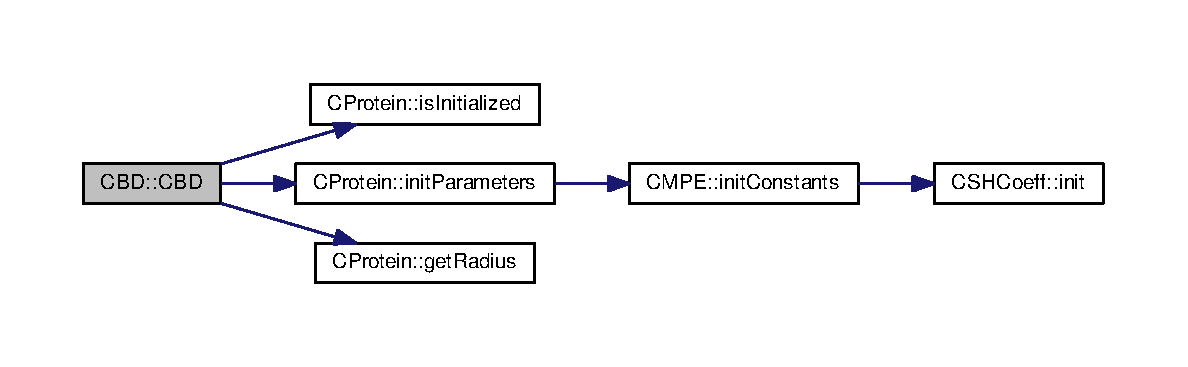
\includegraphics[width=350pt]{classCBD_a9594e15571fc17a65dc1dbe8a0532971_cgraph}
\end{center}
\end{figure}




\subsection{Member Function Documentation}
\hypertarget{classCBD_afa41f280cb3eeb206e6e7c7e99332726}{\index{C\-B\-D@{C\-B\-D}!compute\-Rate@{compute\-Rate}}
\index{compute\-Rate@{compute\-Rate}!CBD@{C\-B\-D}}
\subsubsection[{compute\-Rate}]{\setlength{\rightskip}{0pt plus 5cm}{\bf R\-E\-A\-L} C\-B\-D\-::compute\-Rate (
\begin{DoxyParamCaption}
\item[{int}]{num\-Traj, }
\item[{int}]{n\-Docked}
\end{DoxyParamCaption}
)}}\label{classCBD_afa41f280cb3eeb206e6e7c7e99332726}
compute\-Rate \hypertarget{classCBD_a9ad6f87e7436fa716a470e97f0ec836f}{\index{C\-B\-D@{C\-B\-D}!get\-Rand\-Vec@{get\-Rand\-Vec}}
\index{get\-Rand\-Vec@{get\-Rand\-Vec}!CBD@{C\-B\-D}}
\subsubsection[{get\-Rand\-Vec}]{\setlength{\rightskip}{0pt plus 5cm}static {\bf C\-Pnt} C\-B\-D\-::get\-Rand\-Vec (
\begin{DoxyParamCaption}
\item[{{\bf R\-E\-A\-L}}]{std}
\end{DoxyParamCaption}
)\hspace{0.3cm}{\ttfamily [inline]}, {\ttfamily [static]}}}\label{classCBD_a9ad6f87e7436fa716a470e97f0ec836f}


\hyperlink{classCBD}{C\-B\-D} get\-Rand\-Vec function. 


\begin{DoxyParams}{Parameters}
{\em std} & a floating point of random vector length \\
\hline
\end{DoxyParams}
\begin{DoxyReturn}{Returns}
an \hyperlink{classCPnt}{C\-Pnt} object of random orientation and lenght std 
\end{DoxyReturn}


Here is the call graph for this function\-:
\nopagebreak
\begin{figure}[H]
\begin{center}
\leavevmode
\includegraphics[width=276pt]{classCBD_a9ad6f87e7436fa716a470e97f0ec836f_cgraph}
\end{center}
\end{figure}


\hypertarget{classCBD_a0e59f17fc428ea28a8c8b4c9656a3538}{\index{C\-B\-D@{C\-B\-D}!run@{run}}
\index{run@{run}!CBD@{C\-B\-D}}
\subsubsection[{run}]{\setlength{\rightskip}{0pt plus 5cm}{\bf C\-B\-D\-::\-S\-T\-A\-T\-U\-S} C\-B\-D\-::run (
\begin{DoxyParamCaption}
{}
\end{DoxyParamCaption}
)}}\label{classCBD_a0e59f17fc428ea28a8c8b4c9656a3538}


\hyperlink{classCBD}{C\-B\-D} run function. 

Requires no inputs, performs a run on the B\-D class object \begin{DoxyReturn}{Returns}
an enum of the B\-D run's status, whether it be Escaped, docked or running
\end{DoxyReturn}
run\-: Runs a B\-D simulation for 2 proteins. Initializes one at the origin and the other at some distance b\-\_\-\-D\-I\-S\-T away with random orientation. While the status is R\-U\-N\-N\-I\-N\-G, the system computes forces and then moves the 2nd protein and rotates both while keeping the first fixed at the origin. It prints out the position of each molecule, their distance and the force and torques of the system every 1000 steps. 

Here is the call graph for this function\-:
\nopagebreak
\begin{figure}[H]
\begin{center}
\leavevmode
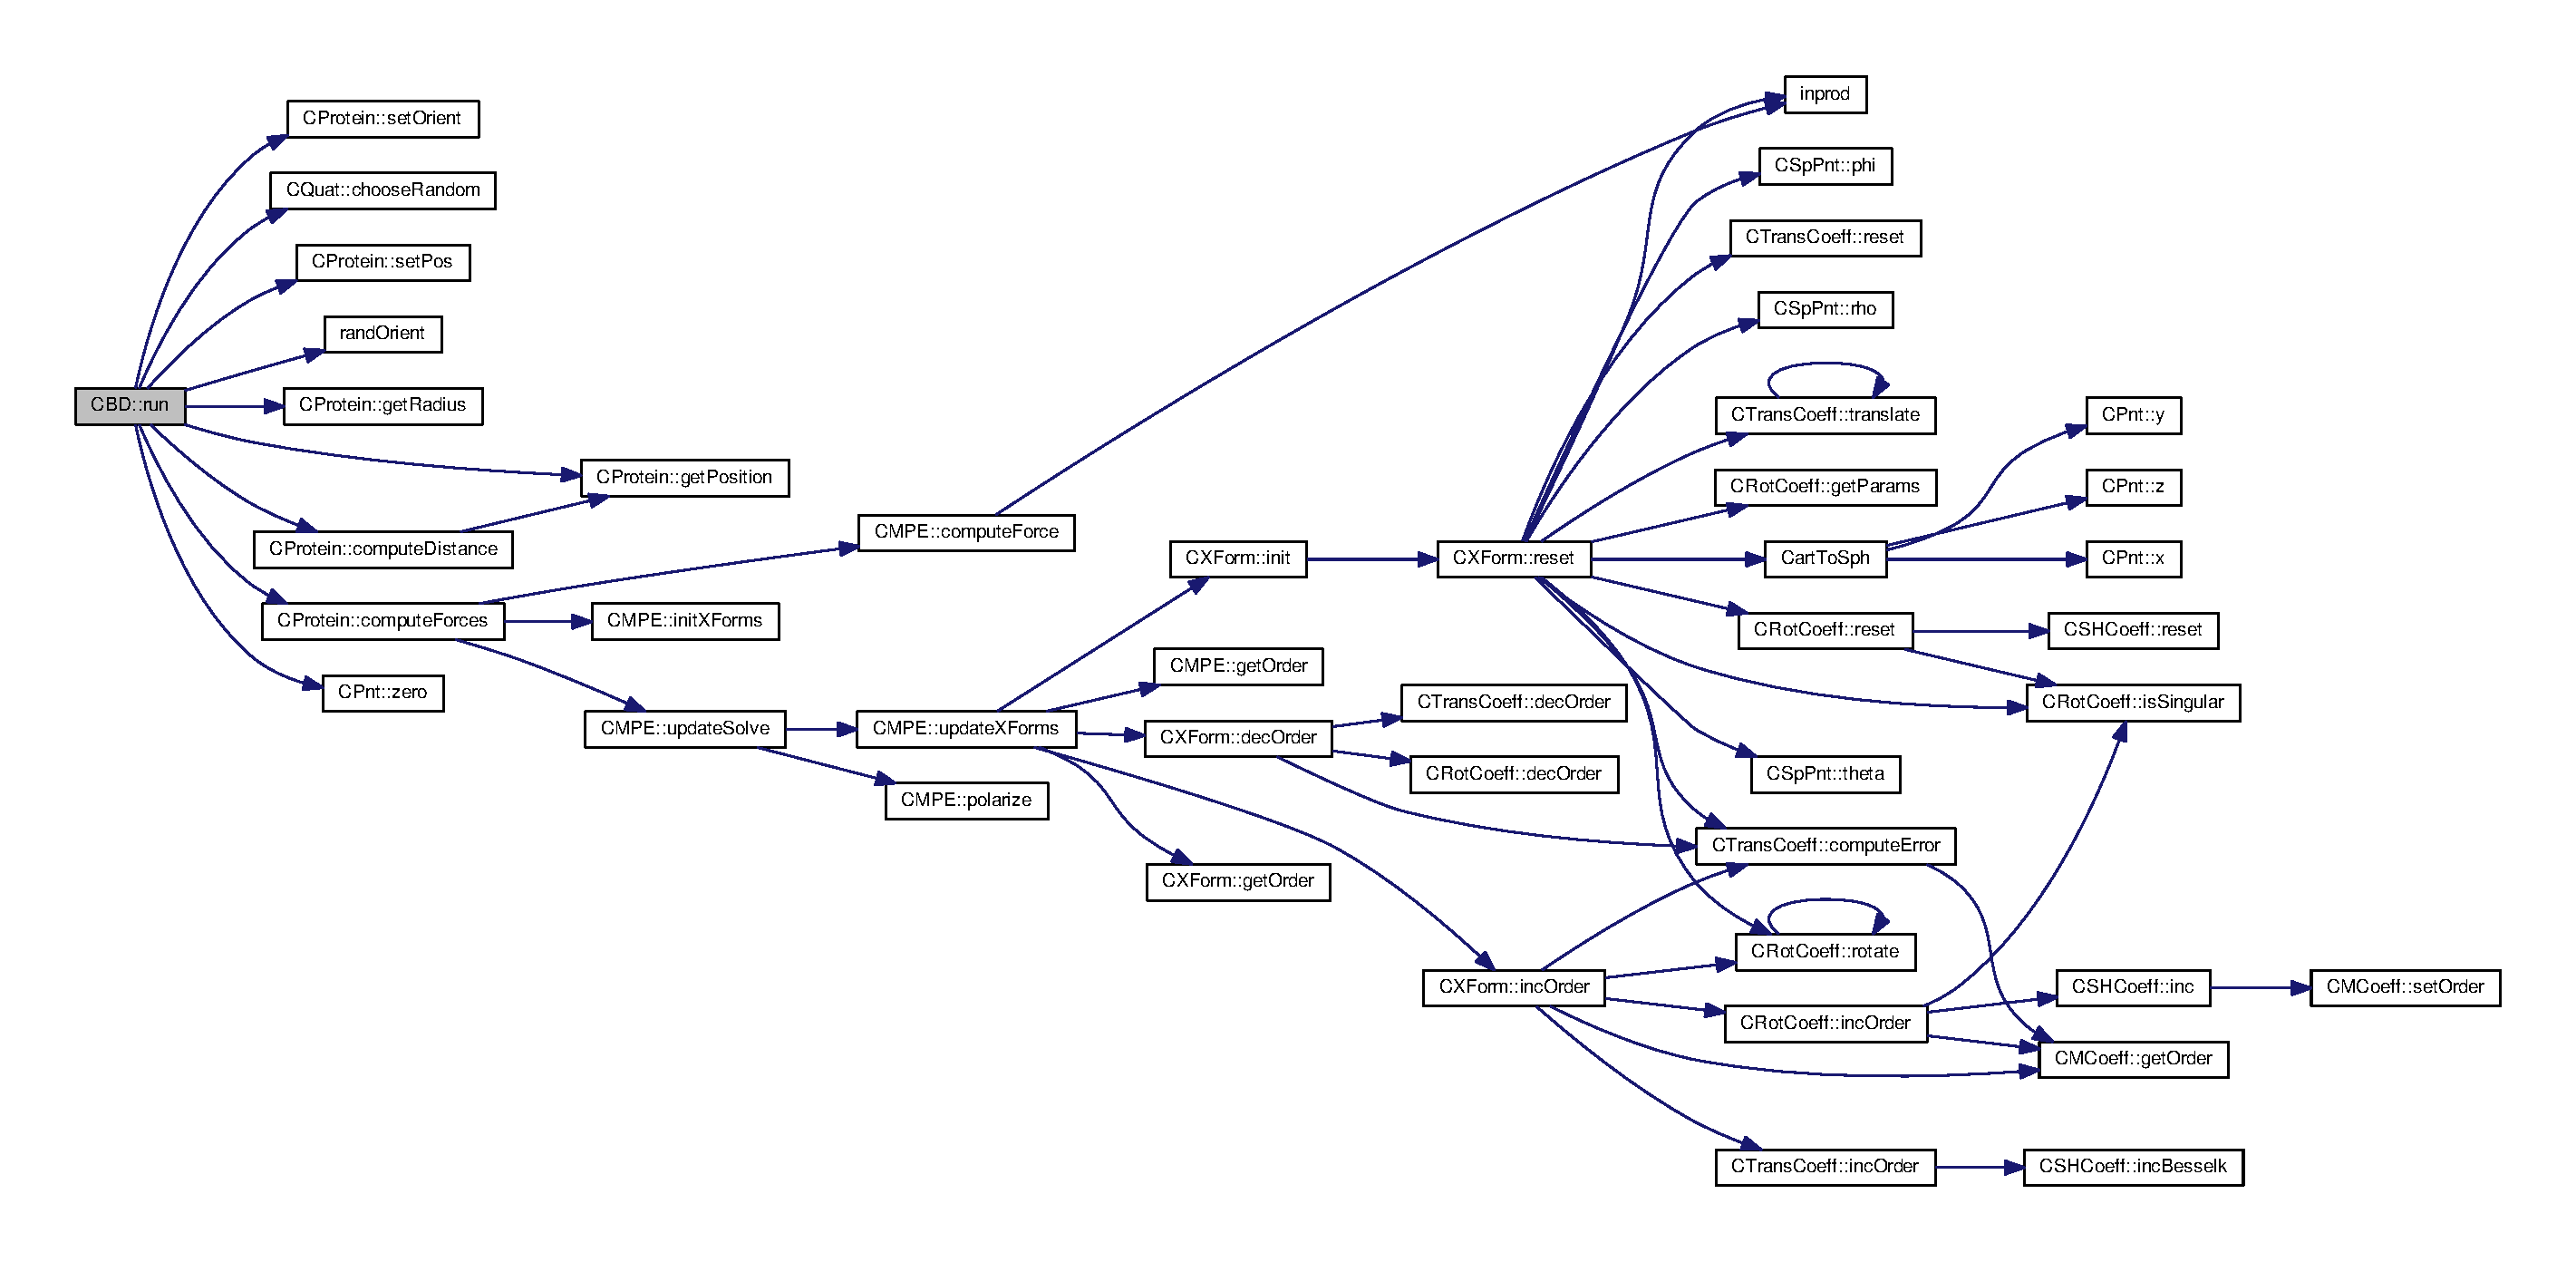
\includegraphics[width=350pt]{classCBD_a0e59f17fc428ea28a8c8b4c9656a3538_cgraph}
\end{center}
\end{figure}




\subsection{Member Data Documentation}
\hypertarget{classCBD_a20beab0b7b100a3d5baf2b3924453641}{\index{C\-B\-D@{C\-B\-D}!S\-T\-A\-T\-U\-S\-\_\-\-S\-T\-R\-I\-N\-G@{S\-T\-A\-T\-U\-S\-\_\-\-S\-T\-R\-I\-N\-G}}
\index{S\-T\-A\-T\-U\-S\-\_\-\-S\-T\-R\-I\-N\-G@{S\-T\-A\-T\-U\-S\-\_\-\-S\-T\-R\-I\-N\-G}!CBD@{C\-B\-D}}
\subsubsection[{S\-T\-A\-T\-U\-S\-\_\-\-S\-T\-R\-I\-N\-G}]{\setlength{\rightskip}{0pt plus 5cm}const char C\-B\-D\-::\-S\-T\-A\-T\-U\-S\-\_\-\-S\-T\-R\-I\-N\-G = \{\char`\"{}E\-S\-C\-A\-P\-E\-D\char`\"{}, \char`\"{}{\bf D\-O\-C\-K\-E\-D}\char`\"{}, \char`\"{}{\bf R\-U\-N\-N\-I\-N\-G}\char`\"{}\}\hspace{0.3cm}{\ttfamily [static]}}}\label{classCBD_a20beab0b7b100a3d5baf2b3924453641}


A string detailing the possible statuses of the system. 



The documentation for this class was generated from the following files\-:\begin{DoxyCompactItemize}
\item 
\hyperlink{BD_8h}{B\-D.\-h}\item 
\hyperlink{BD_8cpp}{B\-D.\-cpp}\end{DoxyCompactItemize}

\hypertarget{classCGradCoeff}{\section{C\-Grad\-Coeff Class Reference}
\label{classCGradCoeff}\index{C\-Grad\-Coeff@{C\-Grad\-Coeff}}
}


The Grad\-Coeff expansion class.  




{\ttfamily \#include $<$gradcoeff.\-h$>$}



Inheritance diagram for C\-Grad\-Coeff\-:\nopagebreak
\begin{figure}[H]
\begin{center}
\leavevmode
\includegraphics[width=148pt]{classCGradCoeff__inherit__graph}
\end{center}
\end{figure}


Collaboration diagram for C\-Grad\-Coeff\-:
\nopagebreak
\begin{figure}[H]
\begin{center}
\leavevmode
\includegraphics[width=148pt]{classCGradCoeff__coll__graph}
\end{center}
\end{figure}
\subsection*{Public Member Functions}
\begin{DoxyCompactItemize}
\item 
\hyperlink{classCGradCoeff_a7c595720bc6386dbe58e7a02a145ed74}{C\-Grad\-Coeff} (int p=0, int res=\hyperlink{mcoeff_8h_ac23f9c13c5d07d9ce386f7a830c35e5a}{N\-\_\-\-P\-O\-L\-E\-S})
\item 
\hyperlink{classCGradCoeff_a08b900b0d57467172733978a44c076f8}{C\-Grad\-Coeff} (const \hyperlink{classCTriCoeff}{C\-Tri\-Coeff} \&G)
\item 
\hyperlink{classCGradCoeff_a41d80b3998f3dfe2a9111ab9f00855fb}{C\-Grad\-Coeff} (const \hyperlink{classCMCoeff}{C\-M\-Coeff} \&M, const \hyperlink{classCSpPnt}{C\-Sp\-Pnt} \&c)
\item 
\hyperlink{classCGradCoeff}{C\-Grad\-Coeff} \hyperlink{classCGradCoeff_ae5711114b36c80f3547ec0857e476500}{sph\-To\-Cart} (const \hyperlink{classCPnt}{C\-Pnt} $\ast$R)
\item 
const \hyperlink{util_8h_a0ef19d29521fc1e3356ea268ba175cfc}{Complex} \hyperlink{classCGradCoeff_ada19e3bbd4f70e5115535cc4365f51b3}{dr} (int n, int m) const 
\item 
const \hyperlink{util_8h_a0ef19d29521fc1e3356ea268ba175cfc}{Complex} \hyperlink{classCGradCoeff_ace80d29d482ccc81d023c2a035dd6022}{dt} (int n, int m) const 
\item 
const \hyperlink{util_8h_a0ef19d29521fc1e3356ea268ba175cfc}{Complex} \hyperlink{classCGradCoeff_a85b5a919cd317987dcb62c7828d179f5}{dp} (int n, int m) const 
\item 
\hyperlink{util_8h_a0ef19d29521fc1e3356ea268ba175cfc}{Complex} \& \hyperlink{classCGradCoeff_acb9edf25321b20753b1e44f1f1a34a04}{dr} (int n, int m)
\item 
\hyperlink{util_8h_a0ef19d29521fc1e3356ea268ba175cfc}{Complex} \& \hyperlink{classCGradCoeff_a7f6f243c58b4de0be441447b4cc1e7e7}{dt} (int n, int m)
\item 
\hyperlink{util_8h_a0ef19d29521fc1e3356ea268ba175cfc}{Complex} \& \hyperlink{classCGradCoeff_afb5b5790c9ddcfbc2b3f88227ca3b74f}{dp} (int n, int m)
\end{DoxyCompactItemize}
\subsection*{Friends}
\begin{DoxyCompactItemize}
\item 
ostream \& \hyperlink{classCGradCoeff_a81f3ceab707183d2313bf86d44b71476}{operator$<$$<$} (ostream \&out, const \hyperlink{classCGradCoeff}{C\-Grad\-Coeff} \&G)
\end{DoxyCompactItemize}
\subsection*{Additional Inherited Members}


\subsection{Detailed Description}
The Grad\-Coeff expansion class. 

The class that contains all details for gradient coefficients. 

\subsection{Constructor \& Destructor Documentation}
\hypertarget{classCGradCoeff_a7c595720bc6386dbe58e7a02a145ed74}{\index{C\-Grad\-Coeff@{C\-Grad\-Coeff}!C\-Grad\-Coeff@{C\-Grad\-Coeff}}
\index{C\-Grad\-Coeff@{C\-Grad\-Coeff}!CGradCoeff@{C\-Grad\-Coeff}}
\subsubsection[{C\-Grad\-Coeff}]{\setlength{\rightskip}{0pt plus 5cm}C\-Grad\-Coeff\-::\-C\-Grad\-Coeff (
\begin{DoxyParamCaption}
\item[{int}]{p = {\ttfamily 0}, }
\item[{int}]{res = {\ttfamily {\bf N\-\_\-\-P\-O\-L\-E\-S}}}
\end{DoxyParamCaption}
)\hspace{0.3cm}{\ttfamily [inline]}}}\label{classCGradCoeff_a7c595720bc6386dbe58e7a02a145ed74}
\hypertarget{classCGradCoeff_a08b900b0d57467172733978a44c076f8}{\index{C\-Grad\-Coeff@{C\-Grad\-Coeff}!C\-Grad\-Coeff@{C\-Grad\-Coeff}}
\index{C\-Grad\-Coeff@{C\-Grad\-Coeff}!CGradCoeff@{C\-Grad\-Coeff}}
\subsubsection[{C\-Grad\-Coeff}]{\setlength{\rightskip}{0pt plus 5cm}C\-Grad\-Coeff\-::\-C\-Grad\-Coeff (
\begin{DoxyParamCaption}
\item[{const {\bf C\-Tri\-Coeff} \&}]{G}
\end{DoxyParamCaption}
)\hspace{0.3cm}{\ttfamily [inline]}}}\label{classCGradCoeff_a08b900b0d57467172733978a44c076f8}
\hypertarget{classCGradCoeff_a41d80b3998f3dfe2a9111ab9f00855fb}{\index{C\-Grad\-Coeff@{C\-Grad\-Coeff}!C\-Grad\-Coeff@{C\-Grad\-Coeff}}
\index{C\-Grad\-Coeff@{C\-Grad\-Coeff}!CGradCoeff@{C\-Grad\-Coeff}}
\subsubsection[{C\-Grad\-Coeff}]{\setlength{\rightskip}{0pt plus 5cm}C\-Grad\-Coeff\-::\-C\-Grad\-Coeff (
\begin{DoxyParamCaption}
\item[{const {\bf C\-M\-Coeff} \&}]{M, }
\item[{const {\bf C\-Sp\-Pnt} \&}]{c}
\end{DoxyParamCaption}
)}}\label{classCGradCoeff_a41d80b3998f3dfe2a9111ab9f00855fb}
\subsection*{File\-: \hyperlink{gradcoeff_8cpp}{gradcoeff.\-cpp}}

\# \subsection*{Date\-: June 2014}

\# \subsection*{Description\-: This file contains the class Grad\-Coeff and its functions}

\# \subsection*{Author\-: Lotan, Felberg}

\# \subsection*{Copyright ( c )}

\# Creating Grad Coefficent class 

Here is the call graph for this function\-:\nopagebreak
\begin{figure}[H]
\begin{center}
\leavevmode
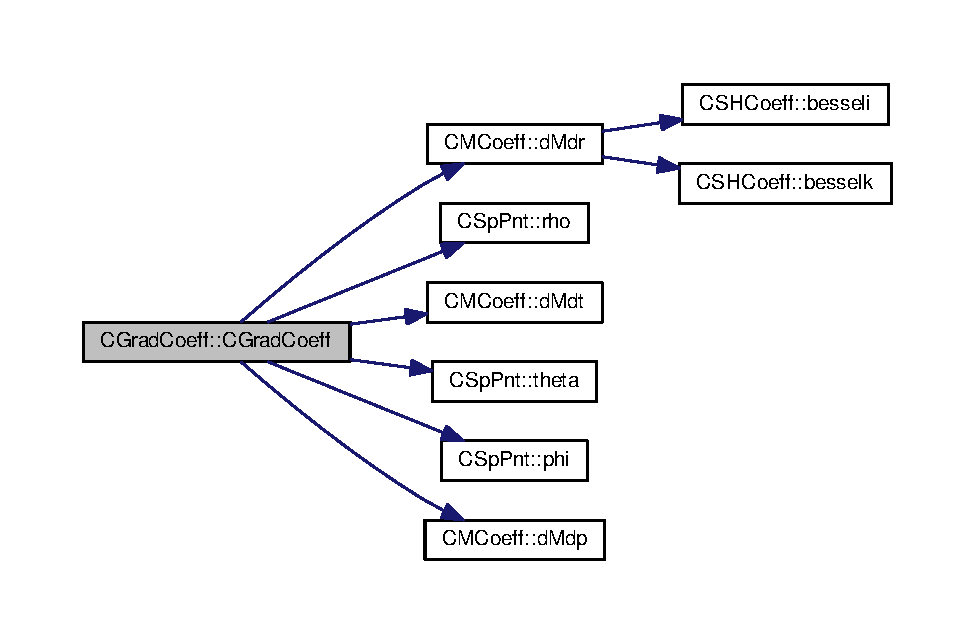
\includegraphics[width=350pt]{classCGradCoeff_a41d80b3998f3dfe2a9111ab9f00855fb_cgraph}
\end{center}
\end{figure}




\subsection{Member Function Documentation}
\hypertarget{classCGradCoeff_a85b5a919cd317987dcb62c7828d179f5}{\index{C\-Grad\-Coeff@{C\-Grad\-Coeff}!dp@{dp}}
\index{dp@{dp}!CGradCoeff@{C\-Grad\-Coeff}}
\subsubsection[{dp}]{\setlength{\rightskip}{0pt plus 5cm}const {\bf Complex} C\-Grad\-Coeff\-::dp (
\begin{DoxyParamCaption}
\item[{int}]{n, }
\item[{int}]{m}
\end{DoxyParamCaption}
) const\hspace{0.3cm}{\ttfamily [inline]}}}\label{classCGradCoeff_a85b5a919cd317987dcb62c7828d179f5}
\hypertarget{classCGradCoeff_afb5b5790c9ddcfbc2b3f88227ca3b74f}{\index{C\-Grad\-Coeff@{C\-Grad\-Coeff}!dp@{dp}}
\index{dp@{dp}!CGradCoeff@{C\-Grad\-Coeff}}
\subsubsection[{dp}]{\setlength{\rightskip}{0pt plus 5cm}{\bf Complex}\& C\-Grad\-Coeff\-::dp (
\begin{DoxyParamCaption}
\item[{int}]{n, }
\item[{int}]{m}
\end{DoxyParamCaption}
)\hspace{0.3cm}{\ttfamily [inline]}}}\label{classCGradCoeff_afb5b5790c9ddcfbc2b3f88227ca3b74f}
\hypertarget{classCGradCoeff_ada19e3bbd4f70e5115535cc4365f51b3}{\index{C\-Grad\-Coeff@{C\-Grad\-Coeff}!dr@{dr}}
\index{dr@{dr}!CGradCoeff@{C\-Grad\-Coeff}}
\subsubsection[{dr}]{\setlength{\rightskip}{0pt plus 5cm}const {\bf Complex} C\-Grad\-Coeff\-::dr (
\begin{DoxyParamCaption}
\item[{int}]{n, }
\item[{int}]{m}
\end{DoxyParamCaption}
) const\hspace{0.3cm}{\ttfamily [inline]}}}\label{classCGradCoeff_ada19e3bbd4f70e5115535cc4365f51b3}
\hypertarget{classCGradCoeff_acb9edf25321b20753b1e44f1f1a34a04}{\index{C\-Grad\-Coeff@{C\-Grad\-Coeff}!dr@{dr}}
\index{dr@{dr}!CGradCoeff@{C\-Grad\-Coeff}}
\subsubsection[{dr}]{\setlength{\rightskip}{0pt plus 5cm}{\bf Complex}\& C\-Grad\-Coeff\-::dr (
\begin{DoxyParamCaption}
\item[{int}]{n, }
\item[{int}]{m}
\end{DoxyParamCaption}
)\hspace{0.3cm}{\ttfamily [inline]}}}\label{classCGradCoeff_acb9edf25321b20753b1e44f1f1a34a04}
\hypertarget{classCGradCoeff_ace80d29d482ccc81d023c2a035dd6022}{\index{C\-Grad\-Coeff@{C\-Grad\-Coeff}!dt@{dt}}
\index{dt@{dt}!CGradCoeff@{C\-Grad\-Coeff}}
\subsubsection[{dt}]{\setlength{\rightskip}{0pt plus 5cm}const {\bf Complex} C\-Grad\-Coeff\-::dt (
\begin{DoxyParamCaption}
\item[{int}]{n, }
\item[{int}]{m}
\end{DoxyParamCaption}
) const\hspace{0.3cm}{\ttfamily [inline]}}}\label{classCGradCoeff_ace80d29d482ccc81d023c2a035dd6022}
\hypertarget{classCGradCoeff_a7f6f243c58b4de0be441447b4cc1e7e7}{\index{C\-Grad\-Coeff@{C\-Grad\-Coeff}!dt@{dt}}
\index{dt@{dt}!CGradCoeff@{C\-Grad\-Coeff}}
\subsubsection[{dt}]{\setlength{\rightskip}{0pt plus 5cm}{\bf Complex}\& C\-Grad\-Coeff\-::dt (
\begin{DoxyParamCaption}
\item[{int}]{n, }
\item[{int}]{m}
\end{DoxyParamCaption}
)\hspace{0.3cm}{\ttfamily [inline]}}}\label{classCGradCoeff_a7f6f243c58b4de0be441447b4cc1e7e7}
\hypertarget{classCGradCoeff_ae5711114b36c80f3547ec0857e476500}{\index{C\-Grad\-Coeff@{C\-Grad\-Coeff}!sph\-To\-Cart@{sph\-To\-Cart}}
\index{sph\-To\-Cart@{sph\-To\-Cart}!CGradCoeff@{C\-Grad\-Coeff}}
\subsubsection[{sph\-To\-Cart}]{\setlength{\rightskip}{0pt plus 5cm}{\bf C\-Grad\-Coeff} C\-Grad\-Coeff\-::sph\-To\-Cart (
\begin{DoxyParamCaption}
\item[{const {\bf C\-Pnt} $\ast$}]{R}
\end{DoxyParamCaption}
)\hspace{0.3cm}{\ttfamily [inline]}}}\label{classCGradCoeff_ae5711114b36c80f3547ec0857e476500}


Here is the call graph for this function\-:\nopagebreak
\begin{figure}[H]
\begin{center}
\leavevmode
\includegraphics[width=288pt]{classCGradCoeff_ae5711114b36c80f3547ec0857e476500_cgraph}
\end{center}
\end{figure}




\subsection{Friends And Related Function Documentation}
\hypertarget{classCGradCoeff_a81f3ceab707183d2313bf86d44b71476}{\index{C\-Grad\-Coeff@{C\-Grad\-Coeff}!operator$<$$<$@{operator$<$$<$}}
\index{operator$<$$<$@{operator$<$$<$}!CGradCoeff@{C\-Grad\-Coeff}}
\subsubsection[{operator$<$$<$}]{\setlength{\rightskip}{0pt plus 5cm}ostream\& {\bf operator}$<$$<$ (
\begin{DoxyParamCaption}
\item[{ostream \&}]{out, }
\item[{const {\bf C\-Grad\-Coeff} \&}]{G}
\end{DoxyParamCaption}
)\hspace{0.3cm}{\ttfamily [friend]}}}\label{classCGradCoeff_a81f3ceab707183d2313bf86d44b71476}


The documentation for this class was generated from the following files\-:\begin{DoxyCompactItemize}
\item 
\hyperlink{gradcoeff_8h}{gradcoeff.\-h}\item 
\hyperlink{gradcoeff_8cpp}{gradcoeff.\-cpp}\end{DoxyCompactItemize}

\hypertarget{classCMCoeff}{\section{C\-M\-Coeff Class Reference}
\label{classCMCoeff}\index{C\-M\-Coeff@{C\-M\-Coeff}}
}


{\ttfamily \#include $<$cmcoeff.\-h$>$}



Inheritance diagram for C\-M\-Coeff\-:
\nopagebreak
\begin{figure}[H]
\begin{center}
\leavevmode
\includegraphics[width=140pt]{classCMCoeff__inherit__graph}
\end{center}
\end{figure}
\subsection*{Public Types}
\begin{DoxyCompactItemize}
\item 
enum \hyperlink{classCMCoeff_a0b490eeb5ba86bc1a95ea1c3b2946478}{T\-Y\-P\-E} \{ \hyperlink{classCMCoeff_a0b490eeb5ba86bc1a95ea1c3b2946478a44c2e68e32e879f210aab9493a0fb48d}{M\-P\-O\-L\-E}, 
\hyperlink{classCMCoeff_a0b490eeb5ba86bc1a95ea1c3b2946478a7620a298f37501509e3a5fec264f0c4f}{M\-P\-O\-L\-E\-\_\-\-K}, 
\hyperlink{classCMCoeff_a0b490eeb5ba86bc1a95ea1c3b2946478a3a2cae46474f6e8cd2151bb47b11002c}{L\-O\-C\-A\-L}, 
\hyperlink{classCMCoeff_a0b490eeb5ba86bc1a95ea1c3b2946478a518645c07b91ad17f9af6fa00ce5042a}{L\-O\-C\-A\-L\-\_\-\-K}
 \}
\end{DoxyCompactItemize}
\subsection*{Public Member Functions}
\begin{DoxyCompactItemize}
\item 
\hyperlink{classCMCoeff_adba776bf8062ab89f60588c138fd562e}{C\-M\-Coeff} (int p) \hyperlink{classCMCoeff_adf49f0bd55b7c496b887f547695aba38}{m\-\_\-p}(p)
\item 
\hyperlink{classCMCoeff_ae5a7fcbb8f989dbbff71d79738fd9356}{C\-M\-Coeff} (const \hyperlink{classCMCoeff}{C\-M\-Coeff} \&M)
\item 
void \hyperlink{classCMCoeff_a2cca0942d27c02cf846810bf465f7ebb}{reset} ()
\item 
const \hyperlink{util_8h_a0ef19d29521fc1e3356ea268ba175cfc}{Complex} \& \hyperlink{classCMCoeff_ae408956538bebea8ad276df0026b2af2}{operator()} (int n, int m) const 
\item 
\hyperlink{classCMCoeff_aee6ebc4dd1ad9096babcaba957db66c7}{C\-M\-Coeff} (const vector$<$ \hyperlink{util_8h_a5821460e95a0800cf9f24c38915cbbde}{R\-E\-A\-L} $>$ \&charges, const vector$<$ \hyperlink{classCPnt}{C\-Pnt} $>$ \&pos, int p, \hyperlink{util_8h_a5821460e95a0800cf9f24c38915cbbde}{R\-E\-A\-L} rad=0.\-0)
\item 
\hyperlink{classCMCoeff_a44f54126d3f90484420f1baf14ed491f}{C\-M\-Coeff} (\hyperlink{util_8h_a5821460e95a0800cf9f24c38915cbbde}{R\-E\-A\-L} ch, const \hyperlink{classCPnt}{C\-Pnt} \&pos, int p, \hyperlink{classCMCoeff_a0b490eeb5ba86bc1a95ea1c3b2946478}{T\-Y\-P\-E} type)
\item 
\hyperlink{classCMCoeff_a52820257419417dd2d18a75e276fd011}{C\-M\-Coeff} (int p=0, int res=\hyperlink{mcoeff_8h_ac23f9c13c5d07d9ce386f7a830c35e5a}{N\-\_\-\-P\-O\-L\-E\-S}, \hyperlink{classCMCoeff_a0b490eeb5ba86bc1a95ea1c3b2946478}{T\-Y\-P\-E} type=\hyperlink{classCMCoeff_a0b490eeb5ba86bc1a95ea1c3b2946478a44c2e68e32e879f210aab9493a0fb48d}{M\-P\-O\-L\-E})
\item 
\hyperlink{classCMCoeff}{C\-M\-Coeff} \& \hyperlink{classCMCoeff_a92c5e5e988695c301c47e3212930a68f}{operator=} (const \hyperlink{classCMCoeff}{C\-M\-Coeff} \&M)
\item 
void \hyperlink{classCMCoeff_a7010837883b56f9b972888bffb6fbb3d}{copy} (const \hyperlink{classCMCoeff}{C\-M\-Coeff} \&M, int p)
\item 
void \hyperlink{classCMCoeff_aba7b82a12360b0789af87a8dda74863b}{copy\-\_\-p} (const \hyperlink{classCMCoeff}{C\-M\-Coeff} \&M, int p)
\item 
\hyperlink{classCMCoeff_ae5a7fcbb8f989dbbff71d79738fd9356}{C\-M\-Coeff} (const \hyperlink{classCMCoeff}{C\-M\-Coeff} \&M)
\item 
\hyperlink{classCMCoeff}{C\-M\-Coeff} \hyperlink{classCMCoeff_aab926cdd2ef1a0f188f82603108296a8}{d\-Mdr} (\hyperlink{util_8h_a5821460e95a0800cf9f24c38915cbbde}{R\-E\-A\-L} r) const 
\item 
\hyperlink{classCMCoeff}{C\-M\-Coeff} \hyperlink{classCMCoeff_a2e9e6517ed48d1758af058f95b5af50c}{d\-Mdt} (\hyperlink{util_8h_a5821460e95a0800cf9f24c38915cbbde}{R\-E\-A\-L} theta, \hyperlink{util_8h_a5821460e95a0800cf9f24c38915cbbde}{R\-E\-A\-L} phi) const 
\item 
\hyperlink{classCMCoeff}{C\-M\-Coeff} \hyperlink{classCMCoeff_a3457ae837d9f8d250757fae3fd69c441}{d\-Mdp} () const 
\item 
void \hyperlink{classCMCoeff_a6e7e750022bf6a6f32dff9092881647c}{recip} ()
\item 
void \hyperlink{classCMCoeff_a5fc4a2ee0ab437bd601fd67ccc5bd43b}{reset} (int p=0)
\item 
void \hyperlink{classCMCoeff_a10d5db85d700255768d091c10fda818c}{reserve} (int p)
\item 
const \hyperlink{util_8h_a0ef19d29521fc1e3356ea268ba175cfc}{Complex} \hyperlink{classCMCoeff_a8776dd638fca3d95f813acb93c7896c7}{operator()} (int n, int m) const 
\item 
\hyperlink{util_8h_a0ef19d29521fc1e3356ea268ba175cfc}{Complex} \& \hyperlink{classCMCoeff_ad6668675df0fa31437bebee2a2b00e0f}{operator()} (int n, int m)
\item 
void \hyperlink{classCMCoeff_a63d33423be766832461e5e20a0f21f66}{operator$\ast$=} (const \hyperlink{util_8h_a5821460e95a0800cf9f24c38915cbbde}{R\-E\-A\-L} C\mbox{[}\hyperlink{mcoeff_8h_ac23f9c13c5d07d9ce386f7a830c35e5a}{N\-\_\-\-P\-O\-L\-E\-S}\mbox{]})
\item 
void \hyperlink{classCMCoeff_ac889bdd0230f6c3f11b8af06915410fe}{operator+=} (const \hyperlink{classCMCoeff}{C\-M\-Coeff} \&E)
\item 
void \hyperlink{classCMCoeff_a28161819e17994b61395e9ddc8532040}{operator-\/=} (const \hyperlink{classCMCoeff}{C\-M\-Coeff} \&E)
\item 
int \hyperlink{classCMCoeff_a4ca84260f5a63a33547ebce310b21c32}{get\-Order} () const 
\item 
void \hyperlink{classCMCoeff_a815a4d1f74b217ea54d9f05f6734004f}{set\-Order} (int p)
\item 
void \hyperlink{classCMCoeff_a99771333750460a0ba9c97f03bdaa6b9}{save\-Undo} ()
\item 
void \hyperlink{classCMCoeff_ae75856578c3de42f457cc6e2af17d1d4}{undo} ()
\item 
void \hyperlink{classCMCoeff_afe4e3e3719dc0808108353ab20b05c23}{output} (int p)
\item 
\hyperlink{util_8h_a5821460e95a0800cf9f24c38915cbbde}{R\-E\-A\-L} \hyperlink{classCMCoeff_a1bf2b3f4bba7f938a9d9d32855737699}{change} () const 
\end{DoxyCompactItemize}
\subsection*{Static Public Member Functions}
\begin{DoxyCompactItemize}
\item 
static \hyperlink{util_8h_a5821460e95a0800cf9f24c38915cbbde}{R\-E\-A\-L} \hyperlink{classCMCoeff_af24efe3725c507a1919b043a5335d9ff}{compute\-Dev} (const \hyperlink{classCMCoeff}{C\-M\-Coeff} \&M1, const \hyperlink{classCMCoeff}{C\-M\-Coeff} \&M2)
\end{DoxyCompactItemize}
\subsection*{Static Public Attributes}
\begin{DoxyCompactItemize}
\item 
static \hyperlink{util_8h_a5821460e95a0800cf9f24c38915cbbde}{R\-E\-A\-L} \hyperlink{classCMCoeff_a512caa3ff1994cbde85011489b8f34ce}{R\-S} = 1.\-0
\item 
static \hyperlink{util_8h_a5821460e95a0800cf9f24c38915cbbde}{R\-E\-A\-L} \hyperlink{classCMCoeff_a7e893ff6deb29f85472663fffd995f42}{I\-R\-S} = 1.\-0
\item 
static \hyperlink{util_8h_a5821460e95a0800cf9f24c38915cbbde}{R\-E\-A\-L} \hyperlink{classCMCoeff_a468f6af1ba4ddbe13561217488c87b40}{K\-A\-P\-P\-A} = 0.\-0
\end{DoxyCompactItemize}
\subsection*{Protected Attributes}
\begin{DoxyCompactItemize}
\item 
\hyperlink{classCMCoeff_a0b490eeb5ba86bc1a95ea1c3b2946478}{T\-Y\-P\-E} \hyperlink{classCMCoeff_afe0cd2c61d33f32a058302fb53c33ccf}{m\-\_\-type}
\item 
vector$<$ \hyperlink{util_8h_a0ef19d29521fc1e3356ea268ba175cfc}{Complex} $>$ \hyperlink{classCMCoeff_a15347641cc66b95ff56bea89f4585edf}{m\-\_\-\-M}
\item 
vector$<$ \hyperlink{util_8h_a0ef19d29521fc1e3356ea268ba175cfc}{Complex} $>$ \hyperlink{classCMCoeff_a2fc4617b2a37d2ca033aea2f5e02b5de}{m\-\_\-\-M\-U}
\item 
int \hyperlink{classCMCoeff_adf49f0bd55b7c496b887f547695aba38}{m\-\_\-p}
\item 
int \hyperlink{classCMCoeff_ac00d5938d669575bf71826ee725ccf46}{m\-\_\-p\-U}
\end{DoxyCompactItemize}
\subsection*{Static Protected Attributes}
\begin{DoxyCompactItemize}
\item 
static int \hyperlink{classCMCoeff_ab1882e6a0df777b1acffadf55844dc92}{I\-D\-X} \mbox{[}2 $\ast$\hyperlink{mcoeff_8h_ac23f9c13c5d07d9ce386f7a830c35e5a}{N\-\_\-\-P\-O\-L\-E\-S}+1\mbox{]}
\end{DoxyCompactItemize}
\subsection*{Friends}
\begin{DoxyCompactItemize}
\item 
ostream \& \hyperlink{classCMCoeff_af219e14c617a293aad17ddf8f055db85}{operator$<$$<$} (ostream \&out, const \hyperlink{classCMCoeff}{C\-M\-Coeff} \&p)
\item 
\hyperlink{classCPnt}{C\-Pnt} \hyperlink{classCMCoeff_a095588ecdb857546a57e3f8f33ec983d}{inprod} (const \hyperlink{classCMCoeff}{C\-M\-Coeff} \&M1, const \hyperlink{classCTriCoeff}{C\-Tri\-Coeff} \&M2)
\item 
\hyperlink{util_8h_a5821460e95a0800cf9f24c38915cbbde}{R\-E\-A\-L} \hyperlink{classCMCoeff_a90c84c259a220e291cebf52d99560c61}{inprod} (const \hyperlink{classCMCoeff}{C\-M\-Coeff} \&M1, const \hyperlink{classCMCoeff}{C\-M\-Coeff} \&M2)
\item 
\hyperlink{classCMCoeff}{C\-M\-Coeff} \hyperlink{classCMCoeff_ab6e8a538afe3d4f8de9c1fa4904479ec}{operator+} (const \hyperlink{classCMCoeff}{C\-M\-Coeff} \&M1, const \hyperlink{classCMCoeff}{C\-M\-Coeff} \&M2)
\item 
\hyperlink{classCMCoeff}{C\-M\-Coeff} \hyperlink{classCMCoeff_a2f5f513c1e1864710b85443edbbc311a}{operator-\/} (const \hyperlink{classCMCoeff}{C\-M\-Coeff} \&M1, const \hyperlink{classCMCoeff}{C\-M\-Coeff} \&M2)
\item 
\hyperlink{classCMCoeff}{C\-M\-Coeff} \hyperlink{classCMCoeff_a794db3eaa0d9cf84e4c8ca1023e4f54a}{operator$\ast$} (const \hyperlink{classCMCoeff}{C\-M\-Coeff} \&M, const \hyperlink{util_8h_a5821460e95a0800cf9f24c38915cbbde}{R\-E\-A\-L} C\mbox{[}\hyperlink{mcoeff_8h_ac23f9c13c5d07d9ce386f7a830c35e5a}{N\-\_\-\-P\-O\-L\-E\-S}\mbox{]})
\item 
\hyperlink{classCMCoeff}{C\-M\-Coeff} \hyperlink{classCMCoeff_a4bebac156440468c712dfce37bc9fc7c}{operator$\ast$} (\hyperlink{util_8h_a5821460e95a0800cf9f24c38915cbbde}{R\-E\-A\-L} s, const \hyperlink{classCMCoeff}{C\-M\-Coeff} \&M)
\item 
\hyperlink{classCMCoeff}{C\-M\-Coeff} \hyperlink{classCMCoeff_a33f855dbf0c86d35853f618e3494db87}{conj} (const \hyperlink{classCMCoeff}{C\-M\-Coeff} \&M)
\end{DoxyCompactItemize}


\subsection{Member Enumeration Documentation}
\hypertarget{classCMCoeff_a0b490eeb5ba86bc1a95ea1c3b2946478}{\index{C\-M\-Coeff@{C\-M\-Coeff}!T\-Y\-P\-E@{T\-Y\-P\-E}}
\index{T\-Y\-P\-E@{T\-Y\-P\-E}!CMCoeff@{C\-M\-Coeff}}
\subsubsection[{T\-Y\-P\-E}]{\setlength{\rightskip}{0pt plus 5cm}enum {\bf C\-M\-Coeff\-::\-T\-Y\-P\-E}}}\label{classCMCoeff_a0b490eeb5ba86bc1a95ea1c3b2946478}
\begin{Desc}
\item[Enumerator\-: ]\par
\begin{description}
\index{M\-P\-O\-L\-E@{M\-P\-O\-L\-E}!C\-M\-Coeff@{C\-M\-Coeff}}\index{C\-M\-Coeff@{C\-M\-Coeff}!M\-P\-O\-L\-E@{M\-P\-O\-L\-E}}\item[{\em 
\hypertarget{classCMCoeff_a0b490eeb5ba86bc1a95ea1c3b2946478a44c2e68e32e879f210aab9493a0fb48d}{M\-P\-O\-L\-E}\label{classCMCoeff_a0b490eeb5ba86bc1a95ea1c3b2946478a44c2e68e32e879f210aab9493a0fb48d}
}]\index{M\-P\-O\-L\-E\-\_\-\-K@{M\-P\-O\-L\-E\-\_\-\-K}!C\-M\-Coeff@{C\-M\-Coeff}}\index{C\-M\-Coeff@{C\-M\-Coeff}!M\-P\-O\-L\-E\-\_\-\-K@{M\-P\-O\-L\-E\-\_\-\-K}}\item[{\em 
\hypertarget{classCMCoeff_a0b490eeb5ba86bc1a95ea1c3b2946478a7620a298f37501509e3a5fec264f0c4f}{M\-P\-O\-L\-E\-\_\-\-K}\label{classCMCoeff_a0b490eeb5ba86bc1a95ea1c3b2946478a7620a298f37501509e3a5fec264f0c4f}
}]\index{L\-O\-C\-A\-L@{L\-O\-C\-A\-L}!C\-M\-Coeff@{C\-M\-Coeff}}\index{C\-M\-Coeff@{C\-M\-Coeff}!L\-O\-C\-A\-L@{L\-O\-C\-A\-L}}\item[{\em 
\hypertarget{classCMCoeff_a0b490eeb5ba86bc1a95ea1c3b2946478a3a2cae46474f6e8cd2151bb47b11002c}{L\-O\-C\-A\-L}\label{classCMCoeff_a0b490eeb5ba86bc1a95ea1c3b2946478a3a2cae46474f6e8cd2151bb47b11002c}
}]\index{L\-O\-C\-A\-L\-\_\-\-K@{L\-O\-C\-A\-L\-\_\-\-K}!C\-M\-Coeff@{C\-M\-Coeff}}\index{C\-M\-Coeff@{C\-M\-Coeff}!L\-O\-C\-A\-L\-\_\-\-K@{L\-O\-C\-A\-L\-\_\-\-K}}\item[{\em 
\hypertarget{classCMCoeff_a0b490eeb5ba86bc1a95ea1c3b2946478a518645c07b91ad17f9af6fa00ce5042a}{L\-O\-C\-A\-L\-\_\-\-K}\label{classCMCoeff_a0b490eeb5ba86bc1a95ea1c3b2946478a518645c07b91ad17f9af6fa00ce5042a}
}]\end{description}
\end{Desc}



\subsection{Constructor \& Destructor Documentation}
\hypertarget{classCMCoeff_adba776bf8062ab89f60588c138fd562e}{\index{C\-M\-Coeff@{C\-M\-Coeff}!C\-M\-Coeff@{C\-M\-Coeff}}
\index{C\-M\-Coeff@{C\-M\-Coeff}!CMCoeff@{C\-M\-Coeff}}
\subsubsection[{C\-M\-Coeff}]{\setlength{\rightskip}{0pt plus 5cm}C\-M\-Coeff\-::\-C\-M\-Coeff (
\begin{DoxyParamCaption}
\item[{int}]{p}
\end{DoxyParamCaption}
)\hspace{0.3cm}{\ttfamily [inline]}}}\label{classCMCoeff_adba776bf8062ab89f60588c138fd562e}
\hypertarget{classCMCoeff_ae5a7fcbb8f989dbbff71d79738fd9356}{\index{C\-M\-Coeff@{C\-M\-Coeff}!C\-M\-Coeff@{C\-M\-Coeff}}
\index{C\-M\-Coeff@{C\-M\-Coeff}!CMCoeff@{C\-M\-Coeff}}
\subsubsection[{C\-M\-Coeff}]{\setlength{\rightskip}{0pt plus 5cm}C\-M\-Coeff\-::\-C\-M\-Coeff (
\begin{DoxyParamCaption}
\item[{const {\bf C\-M\-Coeff} \&}]{M}
\end{DoxyParamCaption}
)\hspace{0.3cm}{\ttfamily [inline]}}}\label{classCMCoeff_ae5a7fcbb8f989dbbff71d79738fd9356}
\hypertarget{classCMCoeff_aee6ebc4dd1ad9096babcaba957db66c7}{\index{C\-M\-Coeff@{C\-M\-Coeff}!C\-M\-Coeff@{C\-M\-Coeff}}
\index{C\-M\-Coeff@{C\-M\-Coeff}!CMCoeff@{C\-M\-Coeff}}
\subsubsection[{C\-M\-Coeff}]{\setlength{\rightskip}{0pt plus 5cm}C\-M\-Coeff\-::\-C\-M\-Coeff (
\begin{DoxyParamCaption}
\item[{const vector$<$ {\bf R\-E\-A\-L} $>$ \&}]{charges, }
\item[{const vector$<$ {\bf C\-Pnt} $>$ \&}]{pos, }
\item[{int}]{p, }
\item[{{\bf R\-E\-A\-L}}]{rad = {\ttfamily 0.0}}
\end{DoxyParamCaption}
)}}\label{classCMCoeff_aee6ebc4dd1ad9096babcaba957db66c7}


Here is the call graph for this function\-:
\nopagebreak
\begin{figure}[H]
\begin{center}
\leavevmode
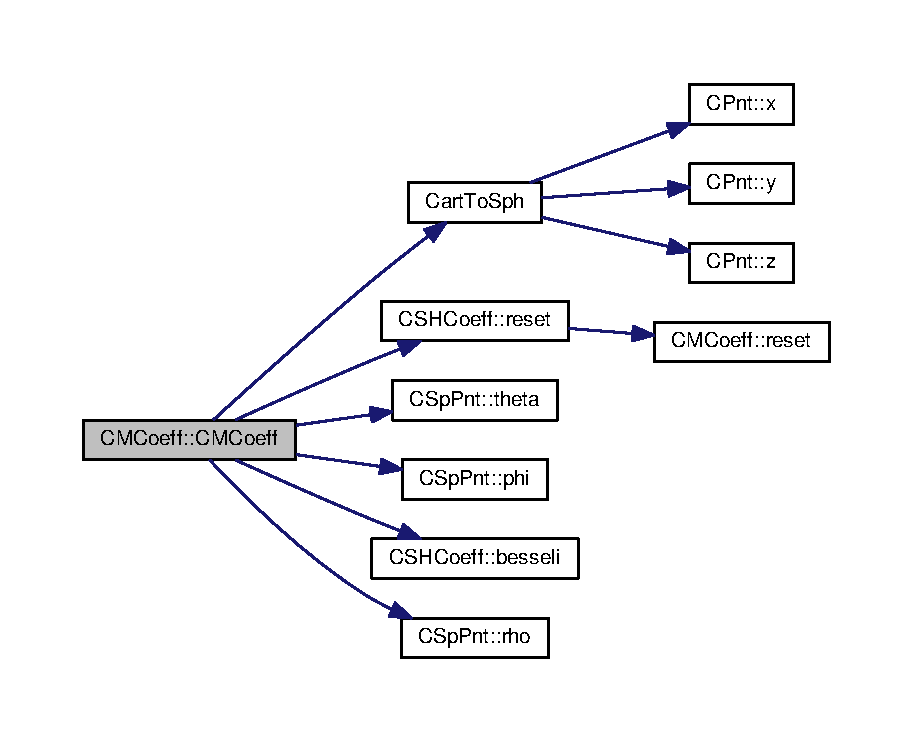
\includegraphics[width=350pt]{classCMCoeff_aee6ebc4dd1ad9096babcaba957db66c7_cgraph}
\end{center}
\end{figure}


\hypertarget{classCMCoeff_a44f54126d3f90484420f1baf14ed491f}{\index{C\-M\-Coeff@{C\-M\-Coeff}!C\-M\-Coeff@{C\-M\-Coeff}}
\index{C\-M\-Coeff@{C\-M\-Coeff}!CMCoeff@{C\-M\-Coeff}}
\subsubsection[{C\-M\-Coeff}]{\setlength{\rightskip}{0pt plus 5cm}C\-M\-Coeff\-::\-C\-M\-Coeff (
\begin{DoxyParamCaption}
\item[{{\bf R\-E\-A\-L}}]{ch, }
\item[{const {\bf C\-Pnt} \&}]{pos, }
\item[{int}]{p, }
\item[{{\bf T\-Y\-P\-E}}]{type}
\end{DoxyParamCaption}
)}}\label{classCMCoeff_a44f54126d3f90484420f1baf14ed491f}


Here is the call graph for this function\-:
\nopagebreak
\begin{figure}[H]
\begin{center}
\leavevmode
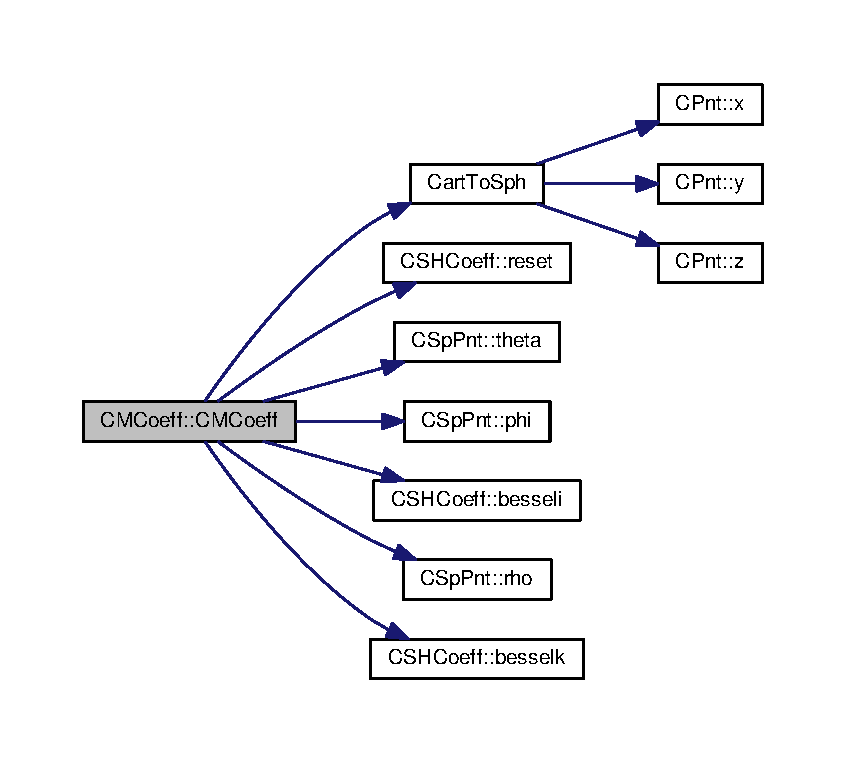
\includegraphics[width=350pt]{classCMCoeff_a44f54126d3f90484420f1baf14ed491f_cgraph}
\end{center}
\end{figure}


\hypertarget{classCMCoeff_a52820257419417dd2d18a75e276fd011}{\index{C\-M\-Coeff@{C\-M\-Coeff}!C\-M\-Coeff@{C\-M\-Coeff}}
\index{C\-M\-Coeff@{C\-M\-Coeff}!CMCoeff@{C\-M\-Coeff}}
\subsubsection[{C\-M\-Coeff}]{\setlength{\rightskip}{0pt plus 5cm}C\-M\-Coeff\-::\-C\-M\-Coeff (
\begin{DoxyParamCaption}
\item[{int}]{p = {\ttfamily 0}, }
\item[{int}]{res = {\ttfamily {\bf N\-\_\-\-P\-O\-L\-E\-S}}, }
\item[{{\bf T\-Y\-P\-E}}]{type = {\ttfamily {\bf M\-P\-O\-L\-E}}}
\end{DoxyParamCaption}
)\hspace{0.3cm}{\ttfamily [inline]}}}\label{classCMCoeff_a52820257419417dd2d18a75e276fd011}


Here is the call graph for this function\-:
\nopagebreak
\begin{figure}[H]
\begin{center}
\leavevmode
\includegraphics[width=256pt]{classCMCoeff_a52820257419417dd2d18a75e276fd011_cgraph}
\end{center}
\end{figure}


\hypertarget{classCMCoeff_ae5a7fcbb8f989dbbff71d79738fd9356}{\index{C\-M\-Coeff@{C\-M\-Coeff}!C\-M\-Coeff@{C\-M\-Coeff}}
\index{C\-M\-Coeff@{C\-M\-Coeff}!CMCoeff@{C\-M\-Coeff}}
\subsubsection[{C\-M\-Coeff}]{\setlength{\rightskip}{0pt plus 5cm}C\-M\-Coeff\-::\-C\-M\-Coeff (
\begin{DoxyParamCaption}
\item[{const {\bf C\-M\-Coeff} \&}]{M}
\end{DoxyParamCaption}
)\hspace{0.3cm}{\ttfamily [inline]}}}\label{classCMCoeff_ae5a7fcbb8f989dbbff71d79738fd9356}


\subsection{Member Function Documentation}
\hypertarget{classCMCoeff_a1bf2b3f4bba7f938a9d9d32855737699}{\index{C\-M\-Coeff@{C\-M\-Coeff}!change@{change}}
\index{change@{change}!CMCoeff@{C\-M\-Coeff}}
\subsubsection[{change}]{\setlength{\rightskip}{0pt plus 5cm}{\bf R\-E\-A\-L} C\-M\-Coeff\-::change (
\begin{DoxyParamCaption}
{}
\end{DoxyParamCaption}
) const\hspace{0.3cm}{\ttfamily [inline]}}}\label{classCMCoeff_a1bf2b3f4bba7f938a9d9d32855737699}


Here is the call graph for this function\-:
\nopagebreak
\begin{figure}[H]
\begin{center}
\leavevmode
\includegraphics[width=328pt]{classCMCoeff_a1bf2b3f4bba7f938a9d9d32855737699_cgraph}
\end{center}
\end{figure}


\hypertarget{classCMCoeff_af24efe3725c507a1919b043a5335d9ff}{\index{C\-M\-Coeff@{C\-M\-Coeff}!compute\-Dev@{compute\-Dev}}
\index{compute\-Dev@{compute\-Dev}!CMCoeff@{C\-M\-Coeff}}
\subsubsection[{compute\-Dev}]{\setlength{\rightskip}{0pt plus 5cm}{\bf R\-E\-A\-L} C\-M\-Coeff\-::compute\-Dev (
\begin{DoxyParamCaption}
\item[{const {\bf C\-M\-Coeff} \&}]{M1, }
\item[{const {\bf C\-M\-Coeff} \&}]{M2}
\end{DoxyParamCaption}
)\hspace{0.3cm}{\ttfamily [inline]}, {\ttfamily [static]}}}\label{classCMCoeff_af24efe3725c507a1919b043a5335d9ff}
\hypertarget{classCMCoeff_a7010837883b56f9b972888bffb6fbb3d}{\index{C\-M\-Coeff@{C\-M\-Coeff}!copy@{copy}}
\index{copy@{copy}!CMCoeff@{C\-M\-Coeff}}
\subsubsection[{copy}]{\setlength{\rightskip}{0pt plus 5cm}void C\-M\-Coeff\-::copy (
\begin{DoxyParamCaption}
\item[{const {\bf C\-M\-Coeff} \&}]{M, }
\item[{int}]{p}
\end{DoxyParamCaption}
)\hspace{0.3cm}{\ttfamily [inline]}}}\label{classCMCoeff_a7010837883b56f9b972888bffb6fbb3d}
\hypertarget{classCMCoeff_aba7b82a12360b0789af87a8dda74863b}{\index{C\-M\-Coeff@{C\-M\-Coeff}!copy\-\_\-p@{copy\-\_\-p}}
\index{copy\-\_\-p@{copy\-\_\-p}!CMCoeff@{C\-M\-Coeff}}
\subsubsection[{copy\-\_\-p}]{\setlength{\rightskip}{0pt plus 5cm}void C\-M\-Coeff\-::copy\-\_\-p (
\begin{DoxyParamCaption}
\item[{const {\bf C\-M\-Coeff} \&}]{M, }
\item[{int}]{p}
\end{DoxyParamCaption}
)\hspace{0.3cm}{\ttfamily [inline]}}}\label{classCMCoeff_aba7b82a12360b0789af87a8dda74863b}
\hypertarget{classCMCoeff_a3457ae837d9f8d250757fae3fd69c441}{\index{C\-M\-Coeff@{C\-M\-Coeff}!d\-Mdp@{d\-Mdp}}
\index{d\-Mdp@{d\-Mdp}!CMCoeff@{C\-M\-Coeff}}
\subsubsection[{d\-Mdp}]{\setlength{\rightskip}{0pt plus 5cm}{\bf C\-M\-Coeff} C\-M\-Coeff\-::d\-Mdp (
\begin{DoxyParamCaption}
{}
\end{DoxyParamCaption}
) const}}\label{classCMCoeff_a3457ae837d9f8d250757fae3fd69c441}
\hypertarget{classCMCoeff_aab926cdd2ef1a0f188f82603108296a8}{\index{C\-M\-Coeff@{C\-M\-Coeff}!d\-Mdr@{d\-Mdr}}
\index{d\-Mdr@{d\-Mdr}!CMCoeff@{C\-M\-Coeff}}
\subsubsection[{d\-Mdr}]{\setlength{\rightskip}{0pt plus 5cm}{\bf C\-M\-Coeff} C\-M\-Coeff\-::d\-Mdr (
\begin{DoxyParamCaption}
\item[{{\bf R\-E\-A\-L}}]{r}
\end{DoxyParamCaption}
) const}}\label{classCMCoeff_aab926cdd2ef1a0f188f82603108296a8}


Here is the call graph for this function\-:
\nopagebreak
\begin{figure}[H]
\begin{center}
\leavevmode
\includegraphics[width=302pt]{classCMCoeff_aab926cdd2ef1a0f188f82603108296a8_cgraph}
\end{center}
\end{figure}


\hypertarget{classCMCoeff_a2e9e6517ed48d1758af058f95b5af50c}{\index{C\-M\-Coeff@{C\-M\-Coeff}!d\-Mdt@{d\-Mdt}}
\index{d\-Mdt@{d\-Mdt}!CMCoeff@{C\-M\-Coeff}}
\subsubsection[{d\-Mdt}]{\setlength{\rightskip}{0pt plus 5cm}{\bf C\-M\-Coeff} C\-M\-Coeff\-::d\-Mdt (
\begin{DoxyParamCaption}
\item[{{\bf R\-E\-A\-L}}]{theta, }
\item[{{\bf R\-E\-A\-L}}]{phi}
\end{DoxyParamCaption}
) const}}\label{classCMCoeff_a2e9e6517ed48d1758af058f95b5af50c}
\hypertarget{classCMCoeff_a4ca84260f5a63a33547ebce310b21c32}{\index{C\-M\-Coeff@{C\-M\-Coeff}!get\-Order@{get\-Order}}
\index{get\-Order@{get\-Order}!CMCoeff@{C\-M\-Coeff}}
\subsubsection[{get\-Order}]{\setlength{\rightskip}{0pt plus 5cm}int C\-M\-Coeff\-::get\-Order (
\begin{DoxyParamCaption}
{}
\end{DoxyParamCaption}
) const\hspace{0.3cm}{\ttfamily [inline]}}}\label{classCMCoeff_a4ca84260f5a63a33547ebce310b21c32}
\hypertarget{classCMCoeff_ae408956538bebea8ad276df0026b2af2}{\index{C\-M\-Coeff@{C\-M\-Coeff}!operator()@{operator()}}
\index{operator()@{operator()}!CMCoeff@{C\-M\-Coeff}}
\subsubsection[{operator()}]{\setlength{\rightskip}{0pt plus 5cm}const {\bf Complex}\& {\bf C\-M\-Coeff\-::operator}() (
\begin{DoxyParamCaption}
\item[{int}]{n, }
\item[{int}]{m}
\end{DoxyParamCaption}
) const\hspace{0.3cm}{\ttfamily [inline]}}}\label{classCMCoeff_ae408956538bebea8ad276df0026b2af2}


Here is the call graph for this function\-:
\nopagebreak
\begin{figure}[H]
\begin{center}
\leavevmode
\includegraphics[width=256pt]{classCMCoeff_ae408956538bebea8ad276df0026b2af2_cgraph}
\end{center}
\end{figure}


\hypertarget{classCMCoeff_a8776dd638fca3d95f813acb93c7896c7}{\index{C\-M\-Coeff@{C\-M\-Coeff}!operator()@{operator()}}
\index{operator()@{operator()}!CMCoeff@{C\-M\-Coeff}}
\subsubsection[{operator()}]{\setlength{\rightskip}{0pt plus 5cm}const {\bf Complex} {\bf C\-M\-Coeff\-::operator}() (
\begin{DoxyParamCaption}
\item[{int}]{n, }
\item[{int}]{m}
\end{DoxyParamCaption}
) const\hspace{0.3cm}{\ttfamily [inline]}}}\label{classCMCoeff_a8776dd638fca3d95f813acb93c7896c7}


Here is the call graph for this function\-:
\nopagebreak
\begin{figure}[H]
\begin{center}
\leavevmode
\includegraphics[width=256pt]{classCMCoeff_a8776dd638fca3d95f813acb93c7896c7_cgraph}
\end{center}
\end{figure}


\hypertarget{classCMCoeff_ad6668675df0fa31437bebee2a2b00e0f}{\index{C\-M\-Coeff@{C\-M\-Coeff}!operator()@{operator()}}
\index{operator()@{operator()}!CMCoeff@{C\-M\-Coeff}}
\subsubsection[{operator()}]{\setlength{\rightskip}{0pt plus 5cm}{\bf Complex}\& {\bf C\-M\-Coeff\-::operator}() (
\begin{DoxyParamCaption}
\item[{int}]{n, }
\item[{int}]{m}
\end{DoxyParamCaption}
)\hspace{0.3cm}{\ttfamily [inline]}}}\label{classCMCoeff_ad6668675df0fa31437bebee2a2b00e0f}
\hypertarget{classCMCoeff_a63d33423be766832461e5e20a0f21f66}{\index{C\-M\-Coeff@{C\-M\-Coeff}!operator$\ast$=@{operator$\ast$=}}
\index{operator$\ast$=@{operator$\ast$=}!CMCoeff@{C\-M\-Coeff}}
\subsubsection[{operator$\ast$=}]{\setlength{\rightskip}{0pt plus 5cm}void {\bf C\-M\-Coeff\-::operator}$\ast$= (
\begin{DoxyParamCaption}
\item[{const {\bf R\-E\-A\-L}}]{C\mbox{[}\-N\-\_\-\-P\-O\-L\-E\-S\mbox{]}}
\end{DoxyParamCaption}
)\hspace{0.3cm}{\ttfamily [inline]}}}\label{classCMCoeff_a63d33423be766832461e5e20a0f21f66}
\hypertarget{classCMCoeff_ac889bdd0230f6c3f11b8af06915410fe}{\index{C\-M\-Coeff@{C\-M\-Coeff}!operator+=@{operator+=}}
\index{operator+=@{operator+=}!CMCoeff@{C\-M\-Coeff}}
\subsubsection[{operator+=}]{\setlength{\rightskip}{0pt plus 5cm}void {\bf C\-M\-Coeff\-::operator}+= (
\begin{DoxyParamCaption}
\item[{const {\bf C\-M\-Coeff} \&}]{E}
\end{DoxyParamCaption}
)\hspace{0.3cm}{\ttfamily [inline]}}}\label{classCMCoeff_ac889bdd0230f6c3f11b8af06915410fe}
\hypertarget{classCMCoeff_a28161819e17994b61395e9ddc8532040}{\index{C\-M\-Coeff@{C\-M\-Coeff}!operator-\/=@{operator-\/=}}
\index{operator-\/=@{operator-\/=}!CMCoeff@{C\-M\-Coeff}}
\subsubsection[{operator-\/=}]{\setlength{\rightskip}{0pt plus 5cm}void {\bf C\-M\-Coeff\-::operator}-\/= (
\begin{DoxyParamCaption}
\item[{const {\bf C\-M\-Coeff} \&}]{E}
\end{DoxyParamCaption}
)\hspace{0.3cm}{\ttfamily [inline]}}}\label{classCMCoeff_a28161819e17994b61395e9ddc8532040}
\hypertarget{classCMCoeff_a92c5e5e988695c301c47e3212930a68f}{\index{C\-M\-Coeff@{C\-M\-Coeff}!operator=@{operator=}}
\index{operator=@{operator=}!CMCoeff@{C\-M\-Coeff}}
\subsubsection[{operator=}]{\setlength{\rightskip}{0pt plus 5cm}{\bf C\-M\-Coeff}\& {\bf C\-M\-Coeff\-::operator}= (
\begin{DoxyParamCaption}
\item[{const {\bf C\-M\-Coeff} \&}]{M}
\end{DoxyParamCaption}
)\hspace{0.3cm}{\ttfamily [inline]}}}\label{classCMCoeff_a92c5e5e988695c301c47e3212930a68f}
\hypertarget{classCMCoeff_afe4e3e3719dc0808108353ab20b05c23}{\index{C\-M\-Coeff@{C\-M\-Coeff}!output@{output}}
\index{output@{output}!CMCoeff@{C\-M\-Coeff}}
\subsubsection[{output}]{\setlength{\rightskip}{0pt plus 5cm}void C\-M\-Coeff\-::output (
\begin{DoxyParamCaption}
\item[{int}]{p}
\end{DoxyParamCaption}
)}}\label{classCMCoeff_afe4e3e3719dc0808108353ab20b05c23}
\hypertarget{classCMCoeff_a6e7e750022bf6a6f32dff9092881647c}{\index{C\-M\-Coeff@{C\-M\-Coeff}!recip@{recip}}
\index{recip@{recip}!CMCoeff@{C\-M\-Coeff}}
\subsubsection[{recip}]{\setlength{\rightskip}{0pt plus 5cm}void C\-M\-Coeff\-::recip (
\begin{DoxyParamCaption}
{}
\end{DoxyParamCaption}
)\hspace{0.3cm}{\ttfamily [inline]}}}\label{classCMCoeff_a6e7e750022bf6a6f32dff9092881647c}
\hypertarget{classCMCoeff_a10d5db85d700255768d091c10fda818c}{\index{C\-M\-Coeff@{C\-M\-Coeff}!reserve@{reserve}}
\index{reserve@{reserve}!CMCoeff@{C\-M\-Coeff}}
\subsubsection[{reserve}]{\setlength{\rightskip}{0pt plus 5cm}void C\-M\-Coeff\-::reserve (
\begin{DoxyParamCaption}
\item[{int}]{p}
\end{DoxyParamCaption}
)\hspace{0.3cm}{\ttfamily [inline]}}}\label{classCMCoeff_a10d5db85d700255768d091c10fda818c}
\hypertarget{classCMCoeff_a2cca0942d27c02cf846810bf465f7ebb}{\index{C\-M\-Coeff@{C\-M\-Coeff}!reset@{reset}}
\index{reset@{reset}!CMCoeff@{C\-M\-Coeff}}
\subsubsection[{reset}]{\setlength{\rightskip}{0pt plus 5cm}void C\-M\-Coeff\-::reset (
\begin{DoxyParamCaption}
{}
\end{DoxyParamCaption}
)\hspace{0.3cm}{\ttfamily [inline]}}}\label{classCMCoeff_a2cca0942d27c02cf846810bf465f7ebb}
\hypertarget{classCMCoeff_a5fc4a2ee0ab437bd601fd67ccc5bd43b}{\index{C\-M\-Coeff@{C\-M\-Coeff}!reset@{reset}}
\index{reset@{reset}!CMCoeff@{C\-M\-Coeff}}
\subsubsection[{reset}]{\setlength{\rightskip}{0pt plus 5cm}void C\-M\-Coeff\-::reset (
\begin{DoxyParamCaption}
\item[{int}]{p = {\ttfamily 0}}
\end{DoxyParamCaption}
)\hspace{0.3cm}{\ttfamily [inline]}}}\label{classCMCoeff_a5fc4a2ee0ab437bd601fd67ccc5bd43b}
\hypertarget{classCMCoeff_a99771333750460a0ba9c97f03bdaa6b9}{\index{C\-M\-Coeff@{C\-M\-Coeff}!save\-Undo@{save\-Undo}}
\index{save\-Undo@{save\-Undo}!CMCoeff@{C\-M\-Coeff}}
\subsubsection[{save\-Undo}]{\setlength{\rightskip}{0pt plus 5cm}void C\-M\-Coeff\-::save\-Undo (
\begin{DoxyParamCaption}
{}
\end{DoxyParamCaption}
)\hspace{0.3cm}{\ttfamily [inline]}}}\label{classCMCoeff_a99771333750460a0ba9c97f03bdaa6b9}
\hypertarget{classCMCoeff_a815a4d1f74b217ea54d9f05f6734004f}{\index{C\-M\-Coeff@{C\-M\-Coeff}!set\-Order@{set\-Order}}
\index{set\-Order@{set\-Order}!CMCoeff@{C\-M\-Coeff}}
\subsubsection[{set\-Order}]{\setlength{\rightskip}{0pt plus 5cm}void C\-M\-Coeff\-::set\-Order (
\begin{DoxyParamCaption}
\item[{int}]{p}
\end{DoxyParamCaption}
)\hspace{0.3cm}{\ttfamily [inline]}}}\label{classCMCoeff_a815a4d1f74b217ea54d9f05f6734004f}
\hypertarget{classCMCoeff_ae75856578c3de42f457cc6e2af17d1d4}{\index{C\-M\-Coeff@{C\-M\-Coeff}!undo@{undo}}
\index{undo@{undo}!CMCoeff@{C\-M\-Coeff}}
\subsubsection[{undo}]{\setlength{\rightskip}{0pt plus 5cm}void C\-M\-Coeff\-::undo (
\begin{DoxyParamCaption}
{}
\end{DoxyParamCaption}
)\hspace{0.3cm}{\ttfamily [inline]}}}\label{classCMCoeff_ae75856578c3de42f457cc6e2af17d1d4}


\subsection{Friends And Related Function Documentation}
\hypertarget{classCMCoeff_a33f855dbf0c86d35853f618e3494db87}{\index{C\-M\-Coeff@{C\-M\-Coeff}!conj@{conj}}
\index{conj@{conj}!CMCoeff@{C\-M\-Coeff}}
\subsubsection[{conj}]{\setlength{\rightskip}{0pt plus 5cm}{\bf C\-M\-Coeff} conj (
\begin{DoxyParamCaption}
\item[{const {\bf C\-M\-Coeff} \&}]{M}
\end{DoxyParamCaption}
)\hspace{0.3cm}{\ttfamily [friend]}}}\label{classCMCoeff_a33f855dbf0c86d35853f618e3494db87}
\hypertarget{classCMCoeff_a095588ecdb857546a57e3f8f33ec983d}{\index{C\-M\-Coeff@{C\-M\-Coeff}!inprod@{inprod}}
\index{inprod@{inprod}!CMCoeff@{C\-M\-Coeff}}
\subsubsection[{inprod}]{\setlength{\rightskip}{0pt plus 5cm}{\bf C\-Pnt} inprod (
\begin{DoxyParamCaption}
\item[{const {\bf C\-M\-Coeff} \&}]{M1, }
\item[{const {\bf C\-Tri\-Coeff} \&}]{M2}
\end{DoxyParamCaption}
)\hspace{0.3cm}{\ttfamily [friend]}}}\label{classCMCoeff_a095588ecdb857546a57e3f8f33ec983d}
\hypertarget{classCMCoeff_a90c84c259a220e291cebf52d99560c61}{\index{C\-M\-Coeff@{C\-M\-Coeff}!inprod@{inprod}}
\index{inprod@{inprod}!CMCoeff@{C\-M\-Coeff}}
\subsubsection[{inprod}]{\setlength{\rightskip}{0pt plus 5cm}{\bf R\-E\-A\-L} inprod (
\begin{DoxyParamCaption}
\item[{const {\bf C\-M\-Coeff} \&}]{M1, }
\item[{const {\bf C\-M\-Coeff} \&}]{M2}
\end{DoxyParamCaption}
)\hspace{0.3cm}{\ttfamily [friend]}}}\label{classCMCoeff_a90c84c259a220e291cebf52d99560c61}
\hypertarget{classCMCoeff_a794db3eaa0d9cf84e4c8ca1023e4f54a}{\index{C\-M\-Coeff@{C\-M\-Coeff}!operator$\ast$@{operator$\ast$}}
\index{operator$\ast$@{operator$\ast$}!CMCoeff@{C\-M\-Coeff}}
\subsubsection[{operator$\ast$}]{\setlength{\rightskip}{0pt plus 5cm}{\bf C\-M\-Coeff} {\bf operator}$\ast$ (
\begin{DoxyParamCaption}
\item[{const {\bf C\-M\-Coeff} \&}]{M, }
\item[{const {\bf R\-E\-A\-L}}]{C\mbox{[}\-N\-\_\-\-P\-O\-L\-E\-S\mbox{]}}
\end{DoxyParamCaption}
)\hspace{0.3cm}{\ttfamily [friend]}}}\label{classCMCoeff_a794db3eaa0d9cf84e4c8ca1023e4f54a}
\hypertarget{classCMCoeff_a4bebac156440468c712dfce37bc9fc7c}{\index{C\-M\-Coeff@{C\-M\-Coeff}!operator$\ast$@{operator$\ast$}}
\index{operator$\ast$@{operator$\ast$}!CMCoeff@{C\-M\-Coeff}}
\subsubsection[{operator$\ast$}]{\setlength{\rightskip}{0pt plus 5cm}{\bf C\-M\-Coeff} {\bf operator}$\ast$ (
\begin{DoxyParamCaption}
\item[{{\bf R\-E\-A\-L}}]{s, }
\item[{const {\bf C\-M\-Coeff} \&}]{M}
\end{DoxyParamCaption}
)\hspace{0.3cm}{\ttfamily [friend]}}}\label{classCMCoeff_a4bebac156440468c712dfce37bc9fc7c}
\hypertarget{classCMCoeff_ab6e8a538afe3d4f8de9c1fa4904479ec}{\index{C\-M\-Coeff@{C\-M\-Coeff}!operator+@{operator+}}
\index{operator+@{operator+}!CMCoeff@{C\-M\-Coeff}}
\subsubsection[{operator+}]{\setlength{\rightskip}{0pt plus 5cm}{\bf C\-M\-Coeff} {\bf operator}+ (
\begin{DoxyParamCaption}
\item[{const {\bf C\-M\-Coeff} \&}]{M1, }
\item[{const {\bf C\-M\-Coeff} \&}]{M2}
\end{DoxyParamCaption}
)\hspace{0.3cm}{\ttfamily [friend]}}}\label{classCMCoeff_ab6e8a538afe3d4f8de9c1fa4904479ec}
\hypertarget{classCMCoeff_a2f5f513c1e1864710b85443edbbc311a}{\index{C\-M\-Coeff@{C\-M\-Coeff}!operator-\/@{operator-\/}}
\index{operator-\/@{operator-\/}!CMCoeff@{C\-M\-Coeff}}
\subsubsection[{operator-\/}]{\setlength{\rightskip}{0pt plus 5cm}{\bf C\-M\-Coeff} {\bf operator}-\/ (
\begin{DoxyParamCaption}
\item[{const {\bf C\-M\-Coeff} \&}]{M1, }
\item[{const {\bf C\-M\-Coeff} \&}]{M2}
\end{DoxyParamCaption}
)\hspace{0.3cm}{\ttfamily [friend]}}}\label{classCMCoeff_a2f5f513c1e1864710b85443edbbc311a}
\hypertarget{classCMCoeff_af219e14c617a293aad17ddf8f055db85}{\index{C\-M\-Coeff@{C\-M\-Coeff}!operator$<$$<$@{operator$<$$<$}}
\index{operator$<$$<$@{operator$<$$<$}!CMCoeff@{C\-M\-Coeff}}
\subsubsection[{operator$<$$<$}]{\setlength{\rightskip}{0pt plus 5cm}ostream\& {\bf operator}$<$$<$ (
\begin{DoxyParamCaption}
\item[{ostream \&}]{out, }
\item[{const {\bf C\-M\-Coeff} \&}]{p}
\end{DoxyParamCaption}
)\hspace{0.3cm}{\ttfamily [friend]}}}\label{classCMCoeff_af219e14c617a293aad17ddf8f055db85}


\subsection{Member Data Documentation}
\hypertarget{classCMCoeff_ab1882e6a0df777b1acffadf55844dc92}{\index{C\-M\-Coeff@{C\-M\-Coeff}!I\-D\-X@{I\-D\-X}}
\index{I\-D\-X@{I\-D\-X}!CMCoeff@{C\-M\-Coeff}}
\subsubsection[{I\-D\-X}]{\setlength{\rightskip}{0pt plus 5cm}int C\-M\-Coeff\-::\-I\-D\-X\hspace{0.3cm}{\ttfamily [static]}, {\ttfamily [protected]}}}\label{classCMCoeff_ab1882e6a0df777b1acffadf55844dc92}
\hypertarget{classCMCoeff_a7e893ff6deb29f85472663fffd995f42}{\index{C\-M\-Coeff@{C\-M\-Coeff}!I\-R\-S@{I\-R\-S}}
\index{I\-R\-S@{I\-R\-S}!CMCoeff@{C\-M\-Coeff}}
\subsubsection[{I\-R\-S}]{\setlength{\rightskip}{0pt plus 5cm}{\bf R\-E\-A\-L} C\-M\-Coeff\-::\-I\-R\-S = 1.\-0\hspace{0.3cm}{\ttfamily [static]}}}\label{classCMCoeff_a7e893ff6deb29f85472663fffd995f42}
\hypertarget{classCMCoeff_a468f6af1ba4ddbe13561217488c87b40}{\index{C\-M\-Coeff@{C\-M\-Coeff}!K\-A\-P\-P\-A@{K\-A\-P\-P\-A}}
\index{K\-A\-P\-P\-A@{K\-A\-P\-P\-A}!CMCoeff@{C\-M\-Coeff}}
\subsubsection[{K\-A\-P\-P\-A}]{\setlength{\rightskip}{0pt plus 5cm}{\bf R\-E\-A\-L} C\-M\-Coeff\-::\-K\-A\-P\-P\-A = 0.\-0\hspace{0.3cm}{\ttfamily [static]}}}\label{classCMCoeff_a468f6af1ba4ddbe13561217488c87b40}
\hypertarget{classCMCoeff_a15347641cc66b95ff56bea89f4585edf}{\index{C\-M\-Coeff@{C\-M\-Coeff}!m\-\_\-\-M@{m\-\_\-\-M}}
\index{m\-\_\-\-M@{m\-\_\-\-M}!CMCoeff@{C\-M\-Coeff}}
\subsubsection[{m\-\_\-\-M}]{\setlength{\rightskip}{0pt plus 5cm}vector$<${\bf Complex}$>$ C\-M\-Coeff\-::m\-\_\-\-M\hspace{0.3cm}{\ttfamily [protected]}}}\label{classCMCoeff_a15347641cc66b95ff56bea89f4585edf}
\hypertarget{classCMCoeff_a2fc4617b2a37d2ca033aea2f5e02b5de}{\index{C\-M\-Coeff@{C\-M\-Coeff}!m\-\_\-\-M\-U@{m\-\_\-\-M\-U}}
\index{m\-\_\-\-M\-U@{m\-\_\-\-M\-U}!CMCoeff@{C\-M\-Coeff}}
\subsubsection[{m\-\_\-\-M\-U}]{\setlength{\rightskip}{0pt plus 5cm}vector$<${\bf Complex}$>$ C\-M\-Coeff\-::m\-\_\-\-M\-U\hspace{0.3cm}{\ttfamily [protected]}}}\label{classCMCoeff_a2fc4617b2a37d2ca033aea2f5e02b5de}
\hypertarget{classCMCoeff_adf49f0bd55b7c496b887f547695aba38}{\index{C\-M\-Coeff@{C\-M\-Coeff}!m\-\_\-p@{m\-\_\-p}}
\index{m\-\_\-p@{m\-\_\-p}!CMCoeff@{C\-M\-Coeff}}
\subsubsection[{m\-\_\-p}]{\setlength{\rightskip}{0pt plus 5cm}int C\-M\-Coeff\-::m\-\_\-p\hspace{0.3cm}{\ttfamily [protected]}}}\label{classCMCoeff_adf49f0bd55b7c496b887f547695aba38}
\hypertarget{classCMCoeff_ac00d5938d669575bf71826ee725ccf46}{\index{C\-M\-Coeff@{C\-M\-Coeff}!m\-\_\-p\-U@{m\-\_\-p\-U}}
\index{m\-\_\-p\-U@{m\-\_\-p\-U}!CMCoeff@{C\-M\-Coeff}}
\subsubsection[{m\-\_\-p\-U}]{\setlength{\rightskip}{0pt plus 5cm}int C\-M\-Coeff\-::m\-\_\-p\-U\hspace{0.3cm}{\ttfamily [protected]}}}\label{classCMCoeff_ac00d5938d669575bf71826ee725ccf46}
\hypertarget{classCMCoeff_afe0cd2c61d33f32a058302fb53c33ccf}{\index{C\-M\-Coeff@{C\-M\-Coeff}!m\-\_\-type@{m\-\_\-type}}
\index{m\-\_\-type@{m\-\_\-type}!CMCoeff@{C\-M\-Coeff}}
\subsubsection[{m\-\_\-type}]{\setlength{\rightskip}{0pt plus 5cm}{\bf T\-Y\-P\-E} C\-M\-Coeff\-::m\-\_\-type\hspace{0.3cm}{\ttfamily [protected]}}}\label{classCMCoeff_afe0cd2c61d33f32a058302fb53c33ccf}
\hypertarget{classCMCoeff_a512caa3ff1994cbde85011489b8f34ce}{\index{C\-M\-Coeff@{C\-M\-Coeff}!R\-S@{R\-S}}
\index{R\-S@{R\-S}!CMCoeff@{C\-M\-Coeff}}
\subsubsection[{R\-S}]{\setlength{\rightskip}{0pt plus 5cm}{\bf R\-E\-A\-L} C\-M\-Coeff\-::\-R\-S = 1.\-0\hspace{0.3cm}{\ttfamily [static]}}}\label{classCMCoeff_a512caa3ff1994cbde85011489b8f34ce}


The documentation for this class was generated from the following files\-:\begin{DoxyCompactItemize}
\item 
\hyperlink{cmcoeff_8h}{cmcoeff.\-h}\item 
\hyperlink{mcoeff_8h}{mcoeff.\-h}\item 
\hyperlink{mcoeff_8cpp}{mcoeff.\-cpp}\end{DoxyCompactItemize}

\hypertarget{classCMPE}{\section{C\-M\-P\-E Class Reference}
\label{classCMPE}\index{C\-M\-P\-E@{C\-M\-P\-E}}
}


The multipole expansion class.  




{\ttfamily \#include $<$mpe.\-h$>$}



Collaboration diagram for C\-M\-P\-E\-:\nopagebreak
\begin{figure}[H]
\begin{center}
\leavevmode
\includegraphics[width=156pt]{classCMPE__coll__graph}
\end{center}
\end{figure}
\subsection*{Public Member Functions}
\begin{DoxyCompactItemize}
\item 
\hyperlink{classCMPE_aee8dd608bd75c7d0415da2746f54acee}{C\-M\-P\-E} (const \hyperlink{classCProtein}{C\-Protein} \&mol)
\begin{DoxyCompactList}\small\item\em \hyperlink{classCMPE}{C\-M\-P\-E} class constructor. \end{DoxyCompactList}\item 
\hyperlink{classCMPE_adbfa1276efd0ce18d73b6943542d6147}{C\-M\-P\-E} (const vector$<$ \hyperlink{util_8h_a5821460e95a0800cf9f24c38915cbbde}{R\-E\-A\-L} $>$ \&charges, const vector$<$ \hyperlink{classCPnt}{C\-Pnt} $>$ \&pos, \hyperlink{util_8h_a5821460e95a0800cf9f24c38915cbbde}{R\-E\-A\-L} rad, int id, int p)
\begin{DoxyCompactList}\small\item\em \hyperlink{classCMPE}{C\-M\-P\-E} class constructor. \end{DoxyCompactList}\item 
void \hyperlink{classCMPE_ae44b4e76215412230e279f34bd5b9fab}{reset} (int p, const \hyperlink{classCQuat}{C\-Quat} \&Q=\hyperlink{classCQuat}{C\-Quat}())
\begin{DoxyCompactList}\small\item\em \hyperlink{classCMPE}{C\-M\-P\-E} reset function. \end{DoxyCompactList}\item 
void \hyperlink{classCMPE_a688ea48a4a13e704fc97e27c0f6dc78a}{set\-Orient} (const \hyperlink{classCQuat}{C\-Quat} \&Q)
\begin{DoxyCompactList}\small\item\em The M\-P\-E set\-Orient function. \end{DoxyCompactList}\item 
const \hyperlink{classCQuat}{C\-Quat} \& \hyperlink{classCMPE_a30f8be93a38d1e9ead77be6bbdc8488f}{get\-Orient} () const 
\begin{DoxyCompactList}\small\item\em The M\-P\-E get\-Orient function. \end{DoxyCompactList}\item 
int \hyperlink{classCMPE_a047394488b2ce41894b336b6a1d8e30a}{get\-Order} () const 
\begin{DoxyCompactList}\small\item\em The M\-P\-E get\-Order function. \end{DoxyCompactList}\item 
\hyperlink{util_8h_a5821460e95a0800cf9f24c38915cbbde}{R\-E\-A\-L} \hyperlink{classCMPE_aa34361e7b83d5e63f866773e9c745588}{get\-Rad} ()
\begin{DoxyCompactList}\small\item\em The M\-P\-E get\-Rad function. \end{DoxyCompactList}\item 
void \hyperlink{classCMPE_a403e7cea8cfca8cb9e76dff5dc396c10}{set\-Order} (int p)
\begin{DoxyCompactList}\small\item\em The M\-P\-E set\-Order function. \end{DoxyCompactList}\item 
void \hyperlink{classCMPE_ad67fb6e520dbc05e63152b18a6363014}{save\-Undo} ()
\begin{DoxyCompactList}\small\item\em The M\-P\-E save\-Undo function. \end{DoxyCompactList}\item 
void \hyperlink{classCMPE_a7033cf96c5b5f6301c6021c97a3f6d36}{undo} ()
\begin{DoxyCompactList}\small\item\em The M\-P\-E undo function. \end{DoxyCompactList}\end{DoxyCompactItemize}
\subsection*{Static Public Member Functions}
\begin{DoxyCompactItemize}
\item 
static void \hyperlink{classCMPE_accac27799cb676fb3160683583a8619e}{init\-Constants} (\hyperlink{util_8h_a5821460e95a0800cf9f24c38915cbbde}{R\-E\-A\-L} kappa, \hyperlink{util_8h_a5821460e95a0800cf9f24c38915cbbde}{R\-E\-A\-L} dielp, \hyperlink{util_8h_a5821460e95a0800cf9f24c38915cbbde}{R\-E\-A\-L} diels, int nmol, \hyperlink{util_8h_a5821460e95a0800cf9f24c38915cbbde}{R\-E\-A\-L} rs)
\begin{DoxyCompactList}\small\item\em \hyperlink{classCMPE}{C\-M\-P\-E} init\-Constants function. \end{DoxyCompactList}\item 
static void \hyperlink{classCMPE_a56b7e4c76e20d5e34393a72cc31f6bb3}{init\-X\-Forms} (const vector$<$ \hyperlink{classCMPE}{C\-M\-P\-E} $\ast$ $>$ \&mpe)
\begin{DoxyCompactList}\small\item\em \hyperlink{classCMPE}{C\-M\-P\-E} init\-X\-Forms function. \end{DoxyCompactList}\item 
static void \hyperlink{classCMPE_ab825df6d8ab377af3715b86e3a495e34}{compute\-Force} (vector$<$ \hyperlink{classCMPE}{C\-M\-P\-E} $\ast$ $>$ \&mpe, const vector$<$ \hyperlink{classCPnt}{C\-Pnt} $\ast$ $>$ \&cen, vector$<$ \hyperlink{util_8h_a5821460e95a0800cf9f24c38915cbbde}{R\-E\-A\-L} $>$ \&pot, vector$<$ \hyperlink{classCPnt}{C\-Pnt} $>$ \&force, vector$<$ \hyperlink{classCPnt}{C\-Pnt} $>$ \&torque)
\begin{DoxyCompactList}\small\item\em \hyperlink{classCMPE}{C\-M\-P\-E} compute\-Force function. \end{DoxyCompactList}\item 
static \hyperlink{util_8h_a5821460e95a0800cf9f24c38915cbbde}{R\-E\-A\-L} \hyperlink{classCMPE_a8a6b260459ff6af55260e2c7897f3bd0}{compute\-Pot\-At} (const vector$<$ \hyperlink{classCMPE}{C\-M\-P\-E} $\ast$ $>$ \&mpe, const vector$<$ \hyperlink{classCPnt}{C\-Pnt} $\ast$ $>$ \&cen, const \hyperlink{classCPnt}{C\-Pnt} \&P)
\begin{DoxyCompactList}\small\item\em \hyperlink{classCMPE}{C\-M\-P\-E} compute\-Pot function. \end{DoxyCompactList}\item 
static void \hyperlink{classCMPE_a46bad2726842ca10071fd004010a6e1b}{solve} (vector$<$ \hyperlink{classCMPE}{C\-M\-P\-E} $\ast$ $>$ \&mpe, const vector$<$ \hyperlink{classCPnt}{C\-Pnt} $\ast$ $>$ \&cen, bool b\-Pot)
\begin{DoxyCompactList}\small\item\em \hyperlink{classCMPE}{C\-M\-P\-E} solve function. \end{DoxyCompactList}\item 
static void \hyperlink{classCMPE_af10ee159904becb5add924aa48df3c56}{reexpand} (const vector$<$ \hyperlink{classCMPE}{C\-M\-P\-E} $\ast$ $>$ \&mpe)
\begin{DoxyCompactList}\small\item\em Function for reexpansion of M\-P\-E. \end{DoxyCompactList}\item 
static void \hyperlink{classCMPE_a70e20d2a606e1bae88c117b15a511e17}{update\-Solve} (vector$<$ \hyperlink{classCMPE}{C\-M\-P\-E} $\ast$ $>$ \&mpe, const vector$<$ \hyperlink{classCPnt}{C\-Pnt} $\ast$ $>$ \&cen)
\begin{DoxyCompactList}\small\item\em Function for updating the solutions of the mutual M\-P\-E. \end{DoxyCompactList}\item 
static void \hyperlink{classCMPE_ab6f4e1fc5fe634c04841e691903d8029}{polarize} (vector$<$ \hyperlink{classCMPE}{C\-M\-P\-E} $\ast$ $>$ \&mpe, bool b\-Pot)
\begin{DoxyCompactList}\small\item\em Function for mutual polarization. \end{DoxyCompactList}\item 
static void \hyperlink{classCMPE_a65d2f19a87b451dbd84bb4b11cbfd571}{update\-X\-Forms} (const vector$<$ \hyperlink{classCPnt}{C\-Pnt} $\ast$ $>$ \&cen, vector$<$ \hyperlink{classCMPE}{C\-M\-P\-E} $\ast$ $>$ \&mpe)
\begin{DoxyCompactList}\small\item\em Function for update\-X\-Forms. \end{DoxyCompactList}\item 
static void \hyperlink{classCMPE_ab494bf000a7dec9410d23a5f47204baf}{compute\-Pair\-Pot} (const vector$<$ \hyperlink{classCMPE}{C\-M\-P\-E} $\ast$ $>$ \&mpe, int i, int j, \hyperlink{util_8h_a5821460e95a0800cf9f24c38915cbbde}{R\-E\-A\-L} \&p1, \hyperlink{util_8h_a5821460e95a0800cf9f24c38915cbbde}{R\-E\-A\-L} \&p2)
\begin{DoxyCompactList}\small\item\em The M\-P\-E compute\-Pair\-Pot function. \end{DoxyCompactList}\item 
static void \hyperlink{classCMPE_a61688da6057b840ca71dacb47db0c0ac}{undo\-X\-Forms} ()
\begin{DoxyCompactList}\small\item\em The M\-P\-E undo\-X\-Forms function. \end{DoxyCompactList}\end{DoxyCompactItemize}
\subsection*{Public Attributes}
\begin{DoxyCompactItemize}
\item 
int \hyperlink{classCMPE_a17b9196644f13740f99675a5a0d8ef23}{ngpol}
\item 
\hyperlink{util_8h_a5821460e95a0800cf9f24c38915cbbde}{R\-E\-A\-L} \hyperlink{classCMPE_afc7b0e78e954f7bb1419864a70c4d0b7}{ngpol\-\_\-t}
\end{DoxyCompactItemize}
\subsection*{Static Public Attributes}
\begin{DoxyCompactItemize}
\item 
static \hyperlink{classCMPE}{C\-M\-P\-E} $\ast$ \hyperlink{classCMPE_a0e97f318480ca27d2a7d608379bd2d03}{tp}
\item 
static bool \hyperlink{classCMPE_a1c612f996b0be31759020f287d3ee7cc}{m\-\_\-b\-Infinite} = false
\begin{DoxyCompactList}\small\item\em Indicates whether simulation for an infinite grid is being performed. \end{DoxyCompactList}\item 
static int \hyperlink{classCMPE_adf1757fa41fec1996e7ca1c7fe6fc9e0}{m\-\_\-unit} = 1
\begin{DoxyCompactList}\small\item\em Unit needed for an infinite grid. Set to 1. \end{DoxyCompactList}\end{DoxyCompactItemize}


\subsection{Detailed Description}
The multipole expansion class. 

The class that contains all details for a multipole expansion. 

\subsection{Constructor \& Destructor Documentation}
\hypertarget{classCMPE_aee8dd608bd75c7d0415da2746f54acee}{\index{C\-M\-P\-E@{C\-M\-P\-E}!C\-M\-P\-E@{C\-M\-P\-E}}
\index{C\-M\-P\-E@{C\-M\-P\-E}!CMPE@{C\-M\-P\-E}}
\subsubsection[{C\-M\-P\-E}]{\setlength{\rightskip}{0pt plus 5cm}C\-M\-P\-E\-::\-C\-M\-P\-E (
\begin{DoxyParamCaption}
\item[{const {\bf C\-Protein} \&}]{mol}
\end{DoxyParamCaption}
)}}\label{classCMPE_aee8dd608bd75c7d0415da2746f54acee}


\hyperlink{classCMPE}{C\-M\-P\-E} class constructor. 


\begin{DoxyParams}{Parameters}
{\em mol} & a pointer to the protein object for which the M\-P\-E will be created \\
\hline
\end{DoxyParams}
\begin{DoxyReturn}{Returns}
an object of the \hyperlink{classCMPE}{C\-M\-P\-E} class
\end{DoxyReturn}
Initialize a multipole expansion with a protein object 

Here is the call graph for this function\-:
\nopagebreak
\begin{figure}[H]
\begin{center}
\leavevmode
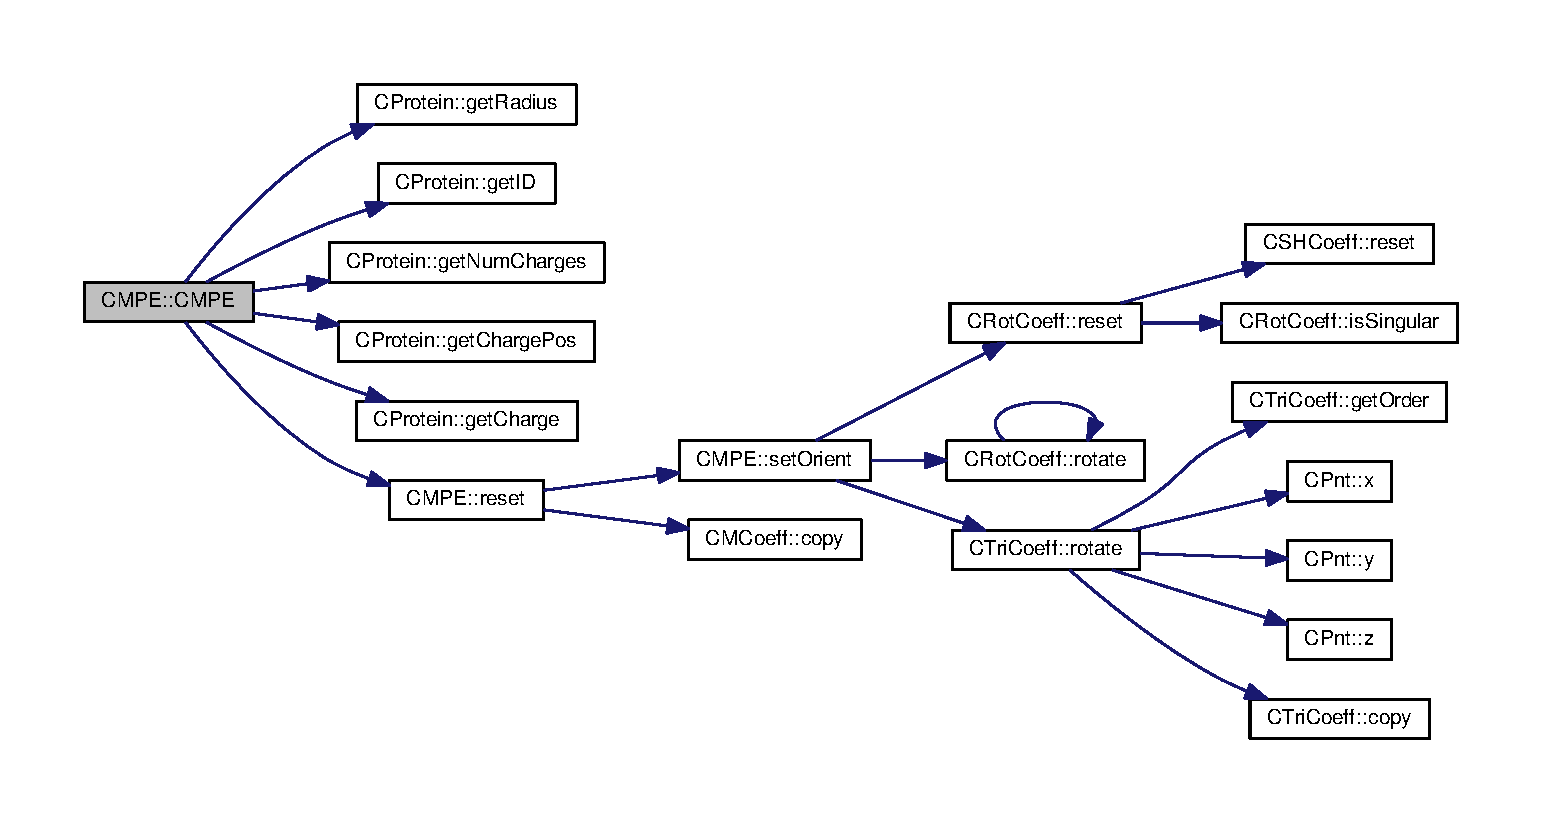
\includegraphics[width=350pt]{classCMPE_aee8dd608bd75c7d0415da2746f54acee_cgraph}
\end{center}
\end{figure}


\hypertarget{classCMPE_adbfa1276efd0ce18d73b6943542d6147}{\index{C\-M\-P\-E@{C\-M\-P\-E}!C\-M\-P\-E@{C\-M\-P\-E}}
\index{C\-M\-P\-E@{C\-M\-P\-E}!CMPE@{C\-M\-P\-E}}
\subsubsection[{C\-M\-P\-E}]{\setlength{\rightskip}{0pt plus 5cm}C\-M\-P\-E\-::\-C\-M\-P\-E (
\begin{DoxyParamCaption}
\item[{const vector$<$ {\bf R\-E\-A\-L} $>$ \&}]{charges, }
\item[{const vector$<$ {\bf C\-Pnt} $>$ \&}]{pos, }
\item[{{\bf R\-E\-A\-L}}]{rad, }
\item[{int}]{id, }
\item[{int}]{p}
\end{DoxyParamCaption}
)}}\label{classCMPE_adbfa1276efd0ce18d73b6943542d6147}


\hyperlink{classCMPE}{C\-M\-P\-E} class constructor. 

Constructs an M\-P\-E object for the computation of self-\/polarization 
\begin{DoxyParams}{Parameters}
{\em charges} & a pointer to a vector of charges \\
\hline
{\em pos} & a pointer to a vector of positions for the aforementioned charges in xyz coords \\
\hline
{\em rad} & a floating point number of the radius of the C\-G sphere containing all charges \\
\hline
{\em id} & an int with numerical I\-D of the C\-G sphere \\
\hline
{\em p} & an int with the number of poles ?? \\
\hline
\end{DoxyParams}
\begin{DoxyReturn}{Returns}
an object of the \hyperlink{classCMPE}{C\-M\-P\-E} class
\end{DoxyReturn}
Create a multipole expansion from a collection of charges. 

Here is the call graph for this function\-:
\nopagebreak
\begin{figure}[H]
\begin{center}
\leavevmode
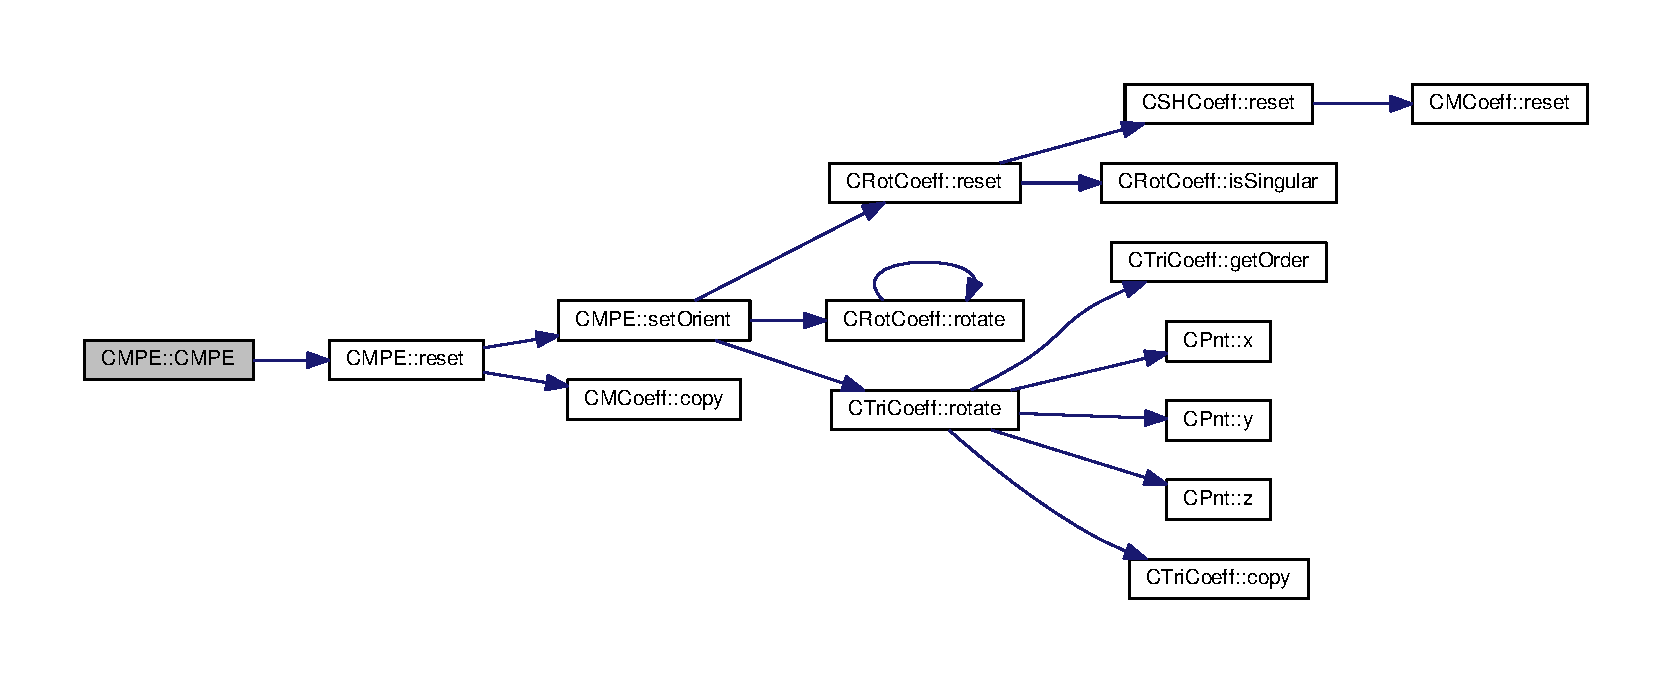
\includegraphics[width=350pt]{classCMPE_adbfa1276efd0ce18d73b6943542d6147_cgraph}
\end{center}
\end{figure}




\subsection{Member Function Documentation}
\hypertarget{classCMPE_ab825df6d8ab377af3715b86e3a495e34}{\index{C\-M\-P\-E@{C\-M\-P\-E}!compute\-Force@{compute\-Force}}
\index{compute\-Force@{compute\-Force}!CMPE@{C\-M\-P\-E}}
\subsubsection[{compute\-Force}]{\setlength{\rightskip}{0pt plus 5cm}void C\-M\-P\-E\-::compute\-Force (
\begin{DoxyParamCaption}
\item[{vector$<$ {\bf C\-M\-P\-E} $\ast$ $>$ \&}]{mpe, }
\item[{const vector$<$ {\bf C\-Pnt} $\ast$ $>$ \&}]{cen, }
\item[{vector$<$ {\bf R\-E\-A\-L} $>$ \&}]{pot, }
\item[{vector$<$ {\bf C\-Pnt} $>$ \&}]{force, }
\item[{vector$<$ {\bf C\-Pnt} $>$ \&}]{torque}
\end{DoxyParamCaption}
)\hspace{0.3cm}{\ttfamily [static]}}}\label{classCMPE_ab825df6d8ab377af3715b86e3a495e34}


\hyperlink{classCMPE}{C\-M\-P\-E} compute\-Force function. 

\hyperlink{classCMPE}{C\-M\-P\-E} function to compute forces and torques on a system 
\begin{DoxyParams}{Parameters}
{\em mpe} & a vector of M\-P\-E objects \\
\hline
{\em cen} & a vector of C\-G object centers in X\-Y\-Z coordinates \\
\hline
{\em pot} & a vector of potentials, one for each molecule \\
\hline
{\em force} & a vector of forces, one for each molecule \\
\hline
{\em torque} & a vector of torques, one for each molecule\\
\hline
\end{DoxyParams}
\hyperlink{classCMPE}{C\-M\-P\-E} function to compute forces and torques on a system 

Here is the call graph for this function\-:
\nopagebreak
\begin{figure}[H]
\begin{center}
\leavevmode
\includegraphics[width=274pt]{classCMPE_ab825df6d8ab377af3715b86e3a495e34_cgraph}
\end{center}
\end{figure}


\hypertarget{classCMPE_ab494bf000a7dec9410d23a5f47204baf}{\index{C\-M\-P\-E@{C\-M\-P\-E}!compute\-Pair\-Pot@{compute\-Pair\-Pot}}
\index{compute\-Pair\-Pot@{compute\-Pair\-Pot}!CMPE@{C\-M\-P\-E}}
\subsubsection[{compute\-Pair\-Pot}]{\setlength{\rightskip}{0pt plus 5cm}void C\-M\-P\-E\-::compute\-Pair\-Pot (
\begin{DoxyParamCaption}
\item[{const vector$<$ {\bf C\-M\-P\-E} $\ast$ $>$ \&}]{mpe, }
\item[{int}]{i, }
\item[{int}]{j, }
\item[{{\bf R\-E\-A\-L} \&}]{p1, }
\item[{{\bf R\-E\-A\-L} \&}]{p2}
\end{DoxyParamCaption}
)\hspace{0.3cm}{\ttfamily [static]}}}\label{classCMPE_ab494bf000a7dec9410d23a5f47204baf}


The M\-P\-E compute\-Pair\-Pot function. 

Function to compute pairwise interaction of two molecules in a system. 
\begin{DoxyParams}{Parameters}
{\em mpe} & a vector of M\-P\-Es, one for each molecule in the system \\
\hline
{\em i} & an integer of the index of the first molecule of interest \\
\hline
{\em j} & an integer of the index of the second molecule of interest \\
\hline
{\em p1} & a floating point of the potential on molecule 1 \\
\hline
{\em p2} & a floating point of the potential on molecule 2\\
\hline
\end{DoxyParams}
Function to compute pairwise interaction of two molecules in a system. 

Here is the call graph for this function\-:
\nopagebreak
\begin{figure}[H]
\begin{center}
\leavevmode
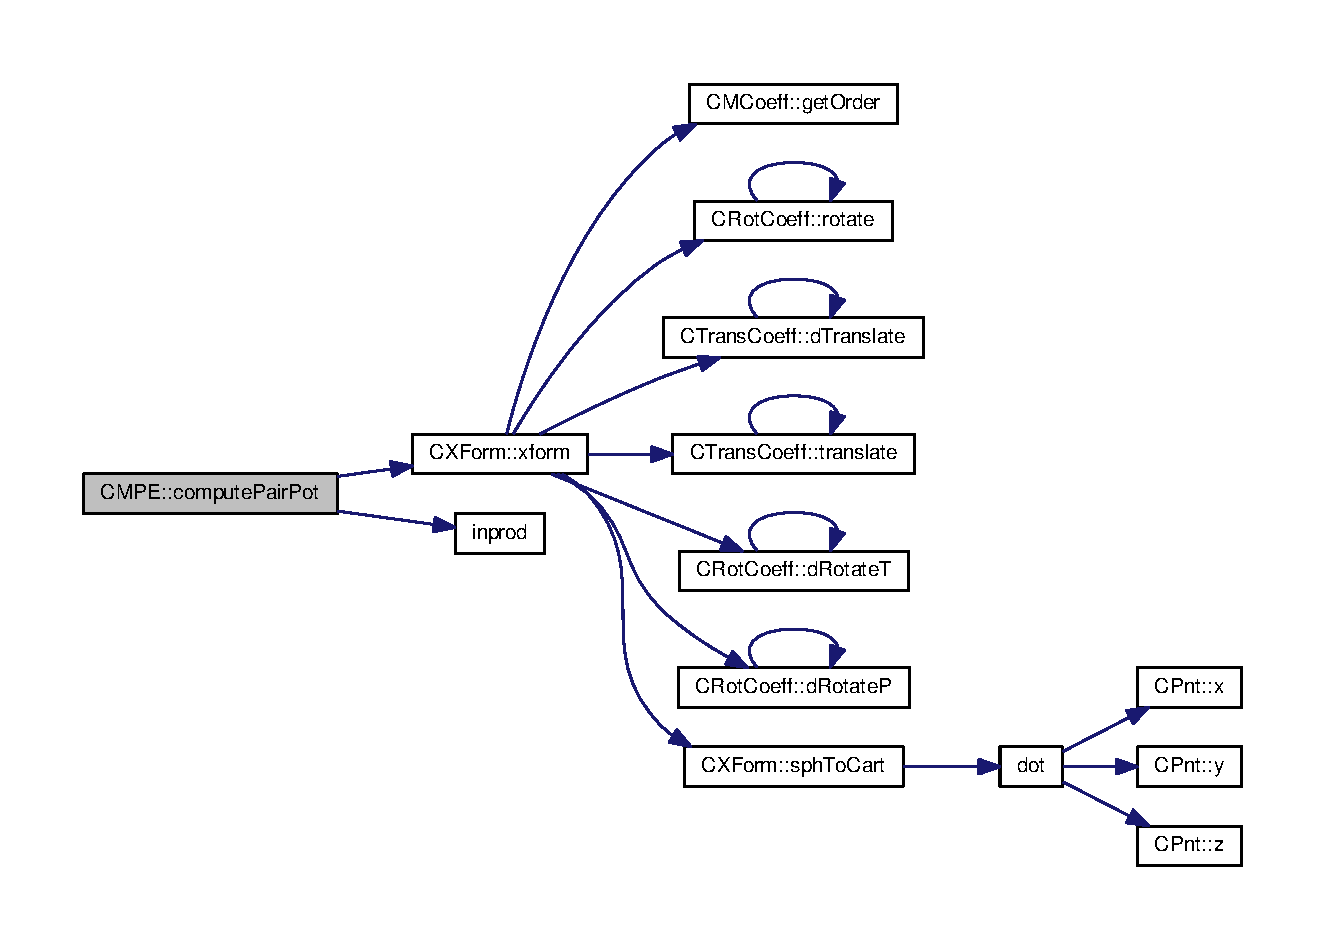
\includegraphics[width=350pt]{classCMPE_ab494bf000a7dec9410d23a5f47204baf_cgraph}
\end{center}
\end{figure}


\hypertarget{classCMPE_a8a6b260459ff6af55260e2c7897f3bd0}{\index{C\-M\-P\-E@{C\-M\-P\-E}!compute\-Pot\-At@{compute\-Pot\-At}}
\index{compute\-Pot\-At@{compute\-Pot\-At}!CMPE@{C\-M\-P\-E}}
\subsubsection[{compute\-Pot\-At}]{\setlength{\rightskip}{0pt plus 5cm}{\bf R\-E\-A\-L} C\-M\-P\-E\-::compute\-Pot\-At (
\begin{DoxyParamCaption}
\item[{const vector$<$ {\bf C\-M\-P\-E} $\ast$ $>$ \&}]{mpe, }
\item[{const vector$<$ {\bf C\-Pnt} $\ast$ $>$ \&}]{cen, }
\item[{const {\bf C\-Pnt} \&}]{P}
\end{DoxyParamCaption}
)\hspace{0.3cm}{\ttfamily [static]}}}\label{classCMPE_a8a6b260459ff6af55260e2c7897f3bd0}


\hyperlink{classCMPE}{C\-M\-P\-E} compute\-Pot function. 

\hyperlink{classCMPE}{C\-M\-P\-E} function to compute potential on a system at a given cartesian point 
\begin{DoxyParams}{Parameters}
{\em mpe} & a vector of M\-P\-E objects \\
\hline
{\em cen} & a vector of C\-G object centers in X\-Y\-Z coordinates \\
\hline
{\em P} & a vector of cartesian coordinates to compute the potential at \\
\hline
\end{DoxyParams}
\begin{DoxyReturn}{Returns}
a floating point of the potential at point P
\end{DoxyReturn}
Function to compute potential on a system at a given cartesian point 

Here is the call graph for this function\-:
\nopagebreak
\begin{figure}[H]
\begin{center}
\leavevmode
\includegraphics[width=320pt]{classCMPE_a8a6b260459ff6af55260e2c7897f3bd0_cgraph}
\end{center}
\end{figure}


\hypertarget{classCMPE_a047394488b2ce41894b336b6a1d8e30a}{\index{C\-M\-P\-E@{C\-M\-P\-E}!get\-Order@{get\-Order}}
\index{get\-Order@{get\-Order}!CMPE@{C\-M\-P\-E}}
\subsubsection[{get\-Order}]{\setlength{\rightskip}{0pt plus 5cm}int C\-M\-P\-E\-::get\-Order (
\begin{DoxyParamCaption}
{}
\end{DoxyParamCaption}
) const\hspace{0.3cm}{\ttfamily [inline]}}}\label{classCMPE_a047394488b2ce41894b336b6a1d8e30a}


The M\-P\-E get\-Order function. 

Function that returns number of poles of the M\-P\-E object \hypertarget{classCMPE_a30f8be93a38d1e9ead77be6bbdc8488f}{\index{C\-M\-P\-E@{C\-M\-P\-E}!get\-Orient@{get\-Orient}}
\index{get\-Orient@{get\-Orient}!CMPE@{C\-M\-P\-E}}
\subsubsection[{get\-Orient}]{\setlength{\rightskip}{0pt plus 5cm}const {\bf C\-Quat}\& C\-M\-P\-E\-::get\-Orient (
\begin{DoxyParamCaption}
{}
\end{DoxyParamCaption}
) const\hspace{0.3cm}{\ttfamily [inline]}}}\label{classCMPE_a30f8be93a38d1e9ead77be6bbdc8488f}


The M\-P\-E get\-Orient function. 

Function that returns the orientation of the M\-P\-E object \hypertarget{classCMPE_aa34361e7b83d5e63f866773e9c745588}{\index{C\-M\-P\-E@{C\-M\-P\-E}!get\-Rad@{get\-Rad}}
\index{get\-Rad@{get\-Rad}!CMPE@{C\-M\-P\-E}}
\subsubsection[{get\-Rad}]{\setlength{\rightskip}{0pt plus 5cm}{\bf R\-E\-A\-L} C\-M\-P\-E\-::get\-Rad (
\begin{DoxyParamCaption}
{}
\end{DoxyParamCaption}
)\hspace{0.3cm}{\ttfamily [inline]}}}\label{classCMPE_aa34361e7b83d5e63f866773e9c745588}


The M\-P\-E get\-Rad function. 

Function that returns the radius of the M\-P\-E object \hypertarget{classCMPE_accac27799cb676fb3160683583a8619e}{\index{C\-M\-P\-E@{C\-M\-P\-E}!init\-Constants@{init\-Constants}}
\index{init\-Constants@{init\-Constants}!CMPE@{C\-M\-P\-E}}
\subsubsection[{init\-Constants}]{\setlength{\rightskip}{0pt plus 5cm}void C\-M\-P\-E\-::init\-Constants (
\begin{DoxyParamCaption}
\item[{{\bf R\-E\-A\-L}}]{kappa, }
\item[{{\bf R\-E\-A\-L}}]{dielp, }
\item[{{\bf R\-E\-A\-L}}]{diels, }
\item[{int}]{nmol, }
\item[{{\bf R\-E\-A\-L}}]{rs}
\end{DoxyParamCaption}
)\hspace{0.3cm}{\ttfamily [static]}}}\label{classCMPE_accac27799cb676fb3160683583a8619e}


\hyperlink{classCMPE}{C\-M\-P\-E} init\-Constants function. 

\hyperlink{classCMPE}{C\-M\-P\-E} function to initialize constants of M\-P\-E functions 
\begin{DoxyParams}{Parameters}
{\em kappa} & a floating point of the inverse debye length \\
\hline
{\em dielp} & a floating point of the dielectric of the protein \\
\hline
{\em diels} & a floating point of the dielectric of the solvent \\
\hline
{\em nmol} & an integer of the number of molecules in the system \\
\hline
{\em rs} & a floating point of a scaling factor for length\\
\hline
\end{DoxyParams}
Initializing parameters for multipole expansion Inputs\-: kappa, dielectric of the protein, water dielectric, the nummber of molecules, average scaling factor 

Here is the call graph for this function\-:\nopagebreak
\begin{figure}[H]
\begin{center}
\leavevmode
\includegraphics[width=308pt]{classCMPE_accac27799cb676fb3160683583a8619e_cgraph}
\end{center}
\end{figure}


\hypertarget{classCMPE_a56b7e4c76e20d5e34393a72cc31f6bb3}{\index{C\-M\-P\-E@{C\-M\-P\-E}!init\-X\-Forms@{init\-X\-Forms}}
\index{init\-X\-Forms@{init\-X\-Forms}!CMPE@{C\-M\-P\-E}}
\subsubsection[{init\-X\-Forms}]{\setlength{\rightskip}{0pt plus 5cm}void C\-M\-P\-E\-::init\-X\-Forms (
\begin{DoxyParamCaption}
\item[{const vector$<$ {\bf C\-M\-P\-E} $\ast$ $>$ \&}]{mpe}
\end{DoxyParamCaption}
)\hspace{0.3cm}{\ttfamily [static]}}}\label{classCMPE_a56b7e4c76e20d5e34393a72cc31f6bb3}


\hyperlink{classCMPE}{C\-M\-P\-E} init\-X\-Forms function. 

\hyperlink{classCMPE}{C\-M\-P\-E} function to initialize the transforms of the M\-P\-E functions 
\begin{DoxyParams}{Parameters}
{\em mpe} & a vector of M\-P\-E objects\\
\hline
\end{DoxyParams}
Initialize transforms. Create a transform for each pair of proteins in the system, using their matrix coefficients. \hypertarget{classCMPE_ab6f4e1fc5fe634c04841e691903d8029}{\index{C\-M\-P\-E@{C\-M\-P\-E}!polarize@{polarize}}
\index{polarize@{polarize}!CMPE@{C\-M\-P\-E}}
\subsubsection[{polarize}]{\setlength{\rightskip}{0pt plus 5cm}void C\-M\-P\-E\-::polarize (
\begin{DoxyParamCaption}
\item[{vector$<$ {\bf C\-M\-P\-E} $\ast$ $>$ \&}]{mpe, }
\item[{bool}]{b\-Pot}
\end{DoxyParamCaption}
)\hspace{0.3cm}{\ttfamily [static]}}}\label{classCMPE_ab6f4e1fc5fe634c04841e691903d8029}


Function for mutual polarization. 

Function of M\-P\-E class that computes the mutual polarization of many bodies in a system, given a vector of the M\-P\-E objects. 
\begin{DoxyParams}{Parameters}
{\em mpe} & a vector of M\-P\-E objects to use for polarization \\
\hline
{\em b\-Pot} & a boolean of whether or not to only compute potential true for only potential, false for gradients as well\\
\hline
\end{DoxyParams}
Routine for mutual polarization. First computes the total number of molecules in the system, then computes the initial mutual polarization and its error. \hypertarget{classCMPE_af10ee159904becb5add924aa48df3c56}{\index{C\-M\-P\-E@{C\-M\-P\-E}!reexpand@{reexpand}}
\index{reexpand@{reexpand}!CMPE@{C\-M\-P\-E}}
\subsubsection[{reexpand}]{\setlength{\rightskip}{0pt plus 5cm}void C\-M\-P\-E\-::reexpand (
\begin{DoxyParamCaption}
\item[{const vector$<$ {\bf C\-M\-P\-E} $\ast$ $>$ \&}]{mpe}
\end{DoxyParamCaption}
)\hspace{0.3cm}{\ttfamily [static]}}}\label{classCMPE_af10ee159904becb5add924aa48df3c56}


Function for reexpansion of M\-P\-E. 

Function of M\-P\-E class that reexpands the input matrix p\-M by the matrix transform, as in E\-Q 46 of paper. 
\begin{DoxyParams}{Parameters}
{\em mpe} & a vector of M\-P\-E objects to use for polarization\\
\hline
\end{DoxyParams}
Function of M\-P\-E class that reexpands the input matrix p\-M by the matrix transform, as in E\-Q 46 of paper. \hypertarget{classCMPE_ae44b4e76215412230e279f34bd5b9fab}{\index{C\-M\-P\-E@{C\-M\-P\-E}!reset@{reset}}
\index{reset@{reset}!CMPE@{C\-M\-P\-E}}
\subsubsection[{reset}]{\setlength{\rightskip}{0pt plus 5cm}void C\-M\-P\-E\-::reset (
\begin{DoxyParamCaption}
\item[{int}]{p, }
\item[{const {\bf C\-Quat} \&}]{Q = {\ttfamily {\bf C\-Quat}()}}
\end{DoxyParamCaption}
)}}\label{classCMPE_ae44b4e76215412230e279f34bd5b9fab}


\hyperlink{classCMPE}{C\-M\-P\-E} reset function. 

\hyperlink{classCMPE}{C\-M\-P\-E} function to reset both the number of poles and the orientation of the multipole expansion 
\begin{DoxyParams}{Parameters}
{\em p} & is an integer number of poles \\
\hline
{\em Q} & is a \hyperlink{classCQuat}{C\-Quat} object for rotating the M\-P\-E\\
\hline
\end{DoxyParams}
\hyperlink{classCMPE}{C\-M\-P\-E} function to reset both the number of poles and the orientation of the multipole expansion 

Here is the call graph for this function\-:
\nopagebreak
\begin{figure}[H]
\begin{center}
\leavevmode
\includegraphics[width=350pt]{classCMPE_ae44b4e76215412230e279f34bd5b9fab_cgraph}
\end{center}
\end{figure}


\hypertarget{classCMPE_ad67fb6e520dbc05e63152b18a6363014}{\index{C\-M\-P\-E@{C\-M\-P\-E}!save\-Undo@{save\-Undo}}
\index{save\-Undo@{save\-Undo}!CMPE@{C\-M\-P\-E}}
\subsubsection[{save\-Undo}]{\setlength{\rightskip}{0pt plus 5cm}void C\-M\-P\-E\-::save\-Undo (
\begin{DoxyParamCaption}
{}
\end{DoxyParamCaption}
)\hspace{0.3cm}{\ttfamily [inline]}}}\label{classCMPE_ad67fb6e520dbc05e63152b18a6363014}


The M\-P\-E save\-Undo function. 

Function that stores everthing in the M\-P\-E object to U parameters incase of future undo \hypertarget{classCMPE_a403e7cea8cfca8cb9e76dff5dc396c10}{\index{C\-M\-P\-E@{C\-M\-P\-E}!set\-Order@{set\-Order}}
\index{set\-Order@{set\-Order}!CMPE@{C\-M\-P\-E}}
\subsubsection[{set\-Order}]{\setlength{\rightskip}{0pt plus 5cm}void C\-M\-P\-E\-::set\-Order (
\begin{DoxyParamCaption}
\item[{int}]{p}
\end{DoxyParamCaption}
)\hspace{0.3cm}{\ttfamily [inline]}}}\label{classCMPE_a403e7cea8cfca8cb9e76dff5dc396c10}


The M\-P\-E set\-Order function. 

Sets the order (number of poles) for the M\-P\-E object 
\begin{DoxyParams}{Parameters}
{\em p} & an int describing the number of poles desired. \\
\hline
\end{DoxyParams}
\hypertarget{classCMPE_a688ea48a4a13e704fc97e27c0f6dc78a}{\index{C\-M\-P\-E@{C\-M\-P\-E}!set\-Orient@{set\-Orient}}
\index{set\-Orient@{set\-Orient}!CMPE@{C\-M\-P\-E}}
\subsubsection[{set\-Orient}]{\setlength{\rightskip}{0pt plus 5cm}void C\-M\-P\-E\-::set\-Orient (
\begin{DoxyParamCaption}
\item[{const {\bf C\-Quat} \&}]{rot}
\end{DoxyParamCaption}
)}}\label{classCMPE_a688ea48a4a13e704fc97e27c0f6dc78a}


The M\-P\-E set\-Orient function. 

Function that sets the orientation of the M\-P\-E object given a quaternion 
\begin{DoxyParams}{Parameters}
{\em Q} & a quaternion object to rotate the M\-P\-E\\
\hline
\end{DoxyParams}
Function that sets the orientation of the M\-P\-E object given a quaternion 

Here is the call graph for this function\-:
\nopagebreak
\begin{figure}[H]
\begin{center}
\leavevmode
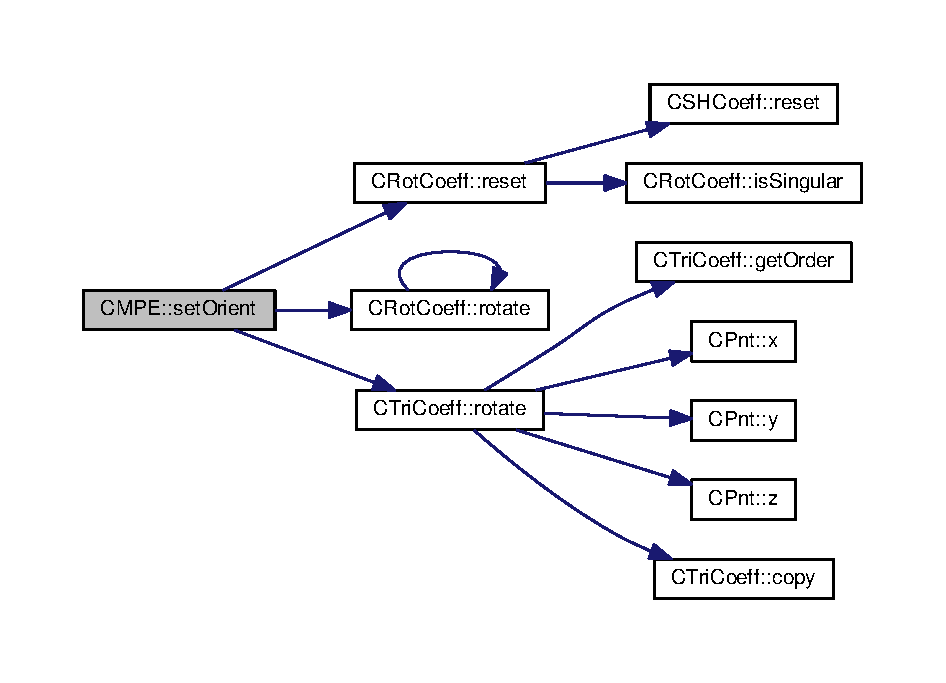
\includegraphics[width=350pt]{classCMPE_a688ea48a4a13e704fc97e27c0f6dc78a_cgraph}
\end{center}
\end{figure}


\hypertarget{classCMPE_a46bad2726842ca10071fd004010a6e1b}{\index{C\-M\-P\-E@{C\-M\-P\-E}!solve@{solve}}
\index{solve@{solve}!CMPE@{C\-M\-P\-E}}
\subsubsection[{solve}]{\setlength{\rightskip}{0pt plus 5cm}void C\-M\-P\-E\-::solve (
\begin{DoxyParamCaption}
\item[{vector$<$ {\bf C\-M\-P\-E} $\ast$ $>$ \&}]{mpe, }
\item[{const vector$<$ {\bf C\-Pnt} $\ast$ $>$ \&}]{cen, }
\item[{bool}]{b\-Pot}
\end{DoxyParamCaption}
)\hspace{0.3cm}{\ttfamily [static]}}}\label{classCMPE_a46bad2726842ca10071fd004010a6e1b}


\hyperlink{classCMPE}{C\-M\-P\-E} solve function. 

A function to run mutual polarization on the system 
\begin{DoxyParams}{Parameters}
{\em mpe} & a vector of M\-P\-E objects\\
\hline
\end{DoxyParams}
A function to run mutual polarization on the system 

Here is the call graph for this function\-:
\nopagebreak
\begin{figure}[H]
\begin{center}
\leavevmode
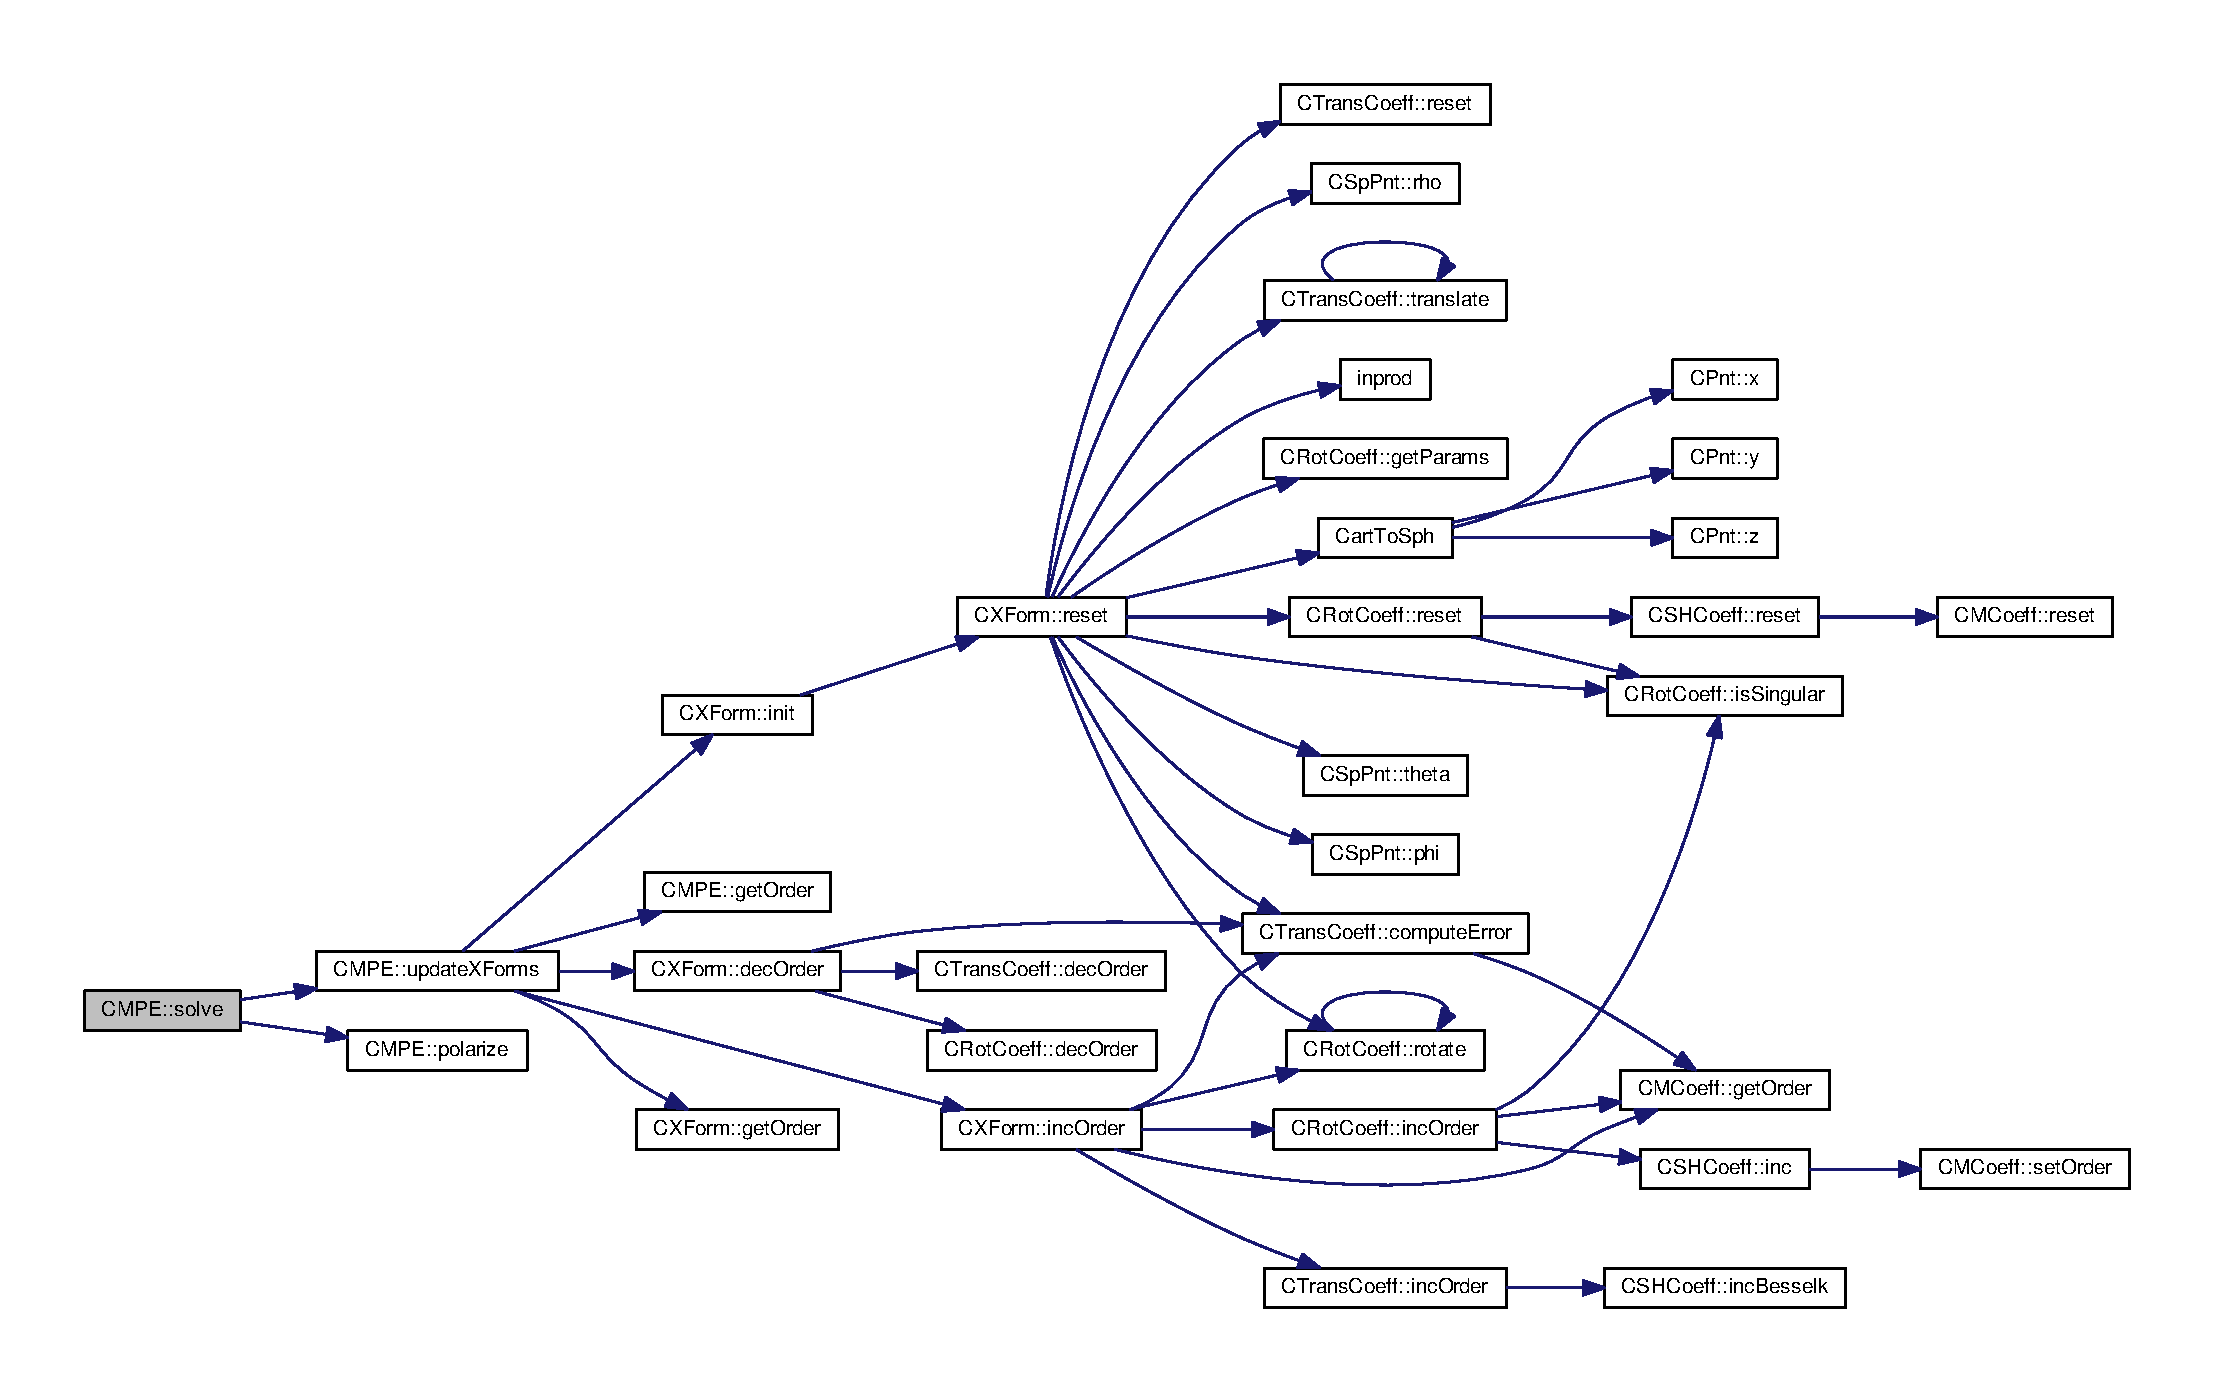
\includegraphics[width=350pt]{classCMPE_a46bad2726842ca10071fd004010a6e1b_cgraph}
\end{center}
\end{figure}


\hypertarget{classCMPE_a7033cf96c5b5f6301c6021c97a3f6d36}{\index{C\-M\-P\-E@{C\-M\-P\-E}!undo@{undo}}
\index{undo@{undo}!CMPE@{C\-M\-P\-E}}
\subsubsection[{undo}]{\setlength{\rightskip}{0pt plus 5cm}void C\-M\-P\-E\-::undo (
\begin{DoxyParamCaption}
{}
\end{DoxyParamCaption}
)\hspace{0.3cm}{\ttfamily [inline]}}}\label{classCMPE_a7033cf96c5b5f6301c6021c97a3f6d36}


The M\-P\-E undo function. 

Function that reverts M\-P\-E object to saved parameters using everything stored in the objects within the class \hypertarget{classCMPE_a61688da6057b840ca71dacb47db0c0ac}{\index{C\-M\-P\-E@{C\-M\-P\-E}!undo\-X\-Forms@{undo\-X\-Forms}}
\index{undo\-X\-Forms@{undo\-X\-Forms}!CMPE@{C\-M\-P\-E}}
\subsubsection[{undo\-X\-Forms}]{\setlength{\rightskip}{0pt plus 5cm}void C\-M\-P\-E\-::undo\-X\-Forms (
\begin{DoxyParamCaption}
{}
\end{DoxyParamCaption}
)\hspace{0.3cm}{\ttfamily [inline]}, {\ttfamily [static]}}}\label{classCMPE_a61688da6057b840ca71dacb47db0c0ac}


The M\-P\-E undo\-X\-Forms function. 

That reverts all transforms between each pair of molecules in the system. \hypertarget{classCMPE_a70e20d2a606e1bae88c117b15a511e17}{\index{C\-M\-P\-E@{C\-M\-P\-E}!update\-Solve@{update\-Solve}}
\index{update\-Solve@{update\-Solve}!CMPE@{C\-M\-P\-E}}
\subsubsection[{update\-Solve}]{\setlength{\rightskip}{0pt plus 5cm}void C\-M\-P\-E\-::update\-Solve (
\begin{DoxyParamCaption}
\item[{vector$<$ {\bf C\-M\-P\-E} $\ast$ $>$ \&}]{mpe, }
\item[{const vector$<$ {\bf C\-Pnt} $\ast$ $>$ \&}]{cen}
\end{DoxyParamCaption}
)\hspace{0.3cm}{\ttfamily [static]}}}\label{classCMPE_a70e20d2a606e1bae88c117b15a511e17}


Function for updating the solutions of the mutual M\-P\-E. 

Update solution to multipole expansion. Calls Transforms and polarize schemes. 
\begin{DoxyParams}{Parameters}
{\em mpe} & a vector of M\-P\-E objects to use for polarization \\
\hline
{\em cen} & a vector of centers of C\-G spheres\\
\hline
\end{DoxyParams}
Update solution to multipole expansion. Calls Transforms and polarize schemes. 

Here is the call graph for this function\-:
\nopagebreak
\begin{figure}[H]
\begin{center}
\leavevmode
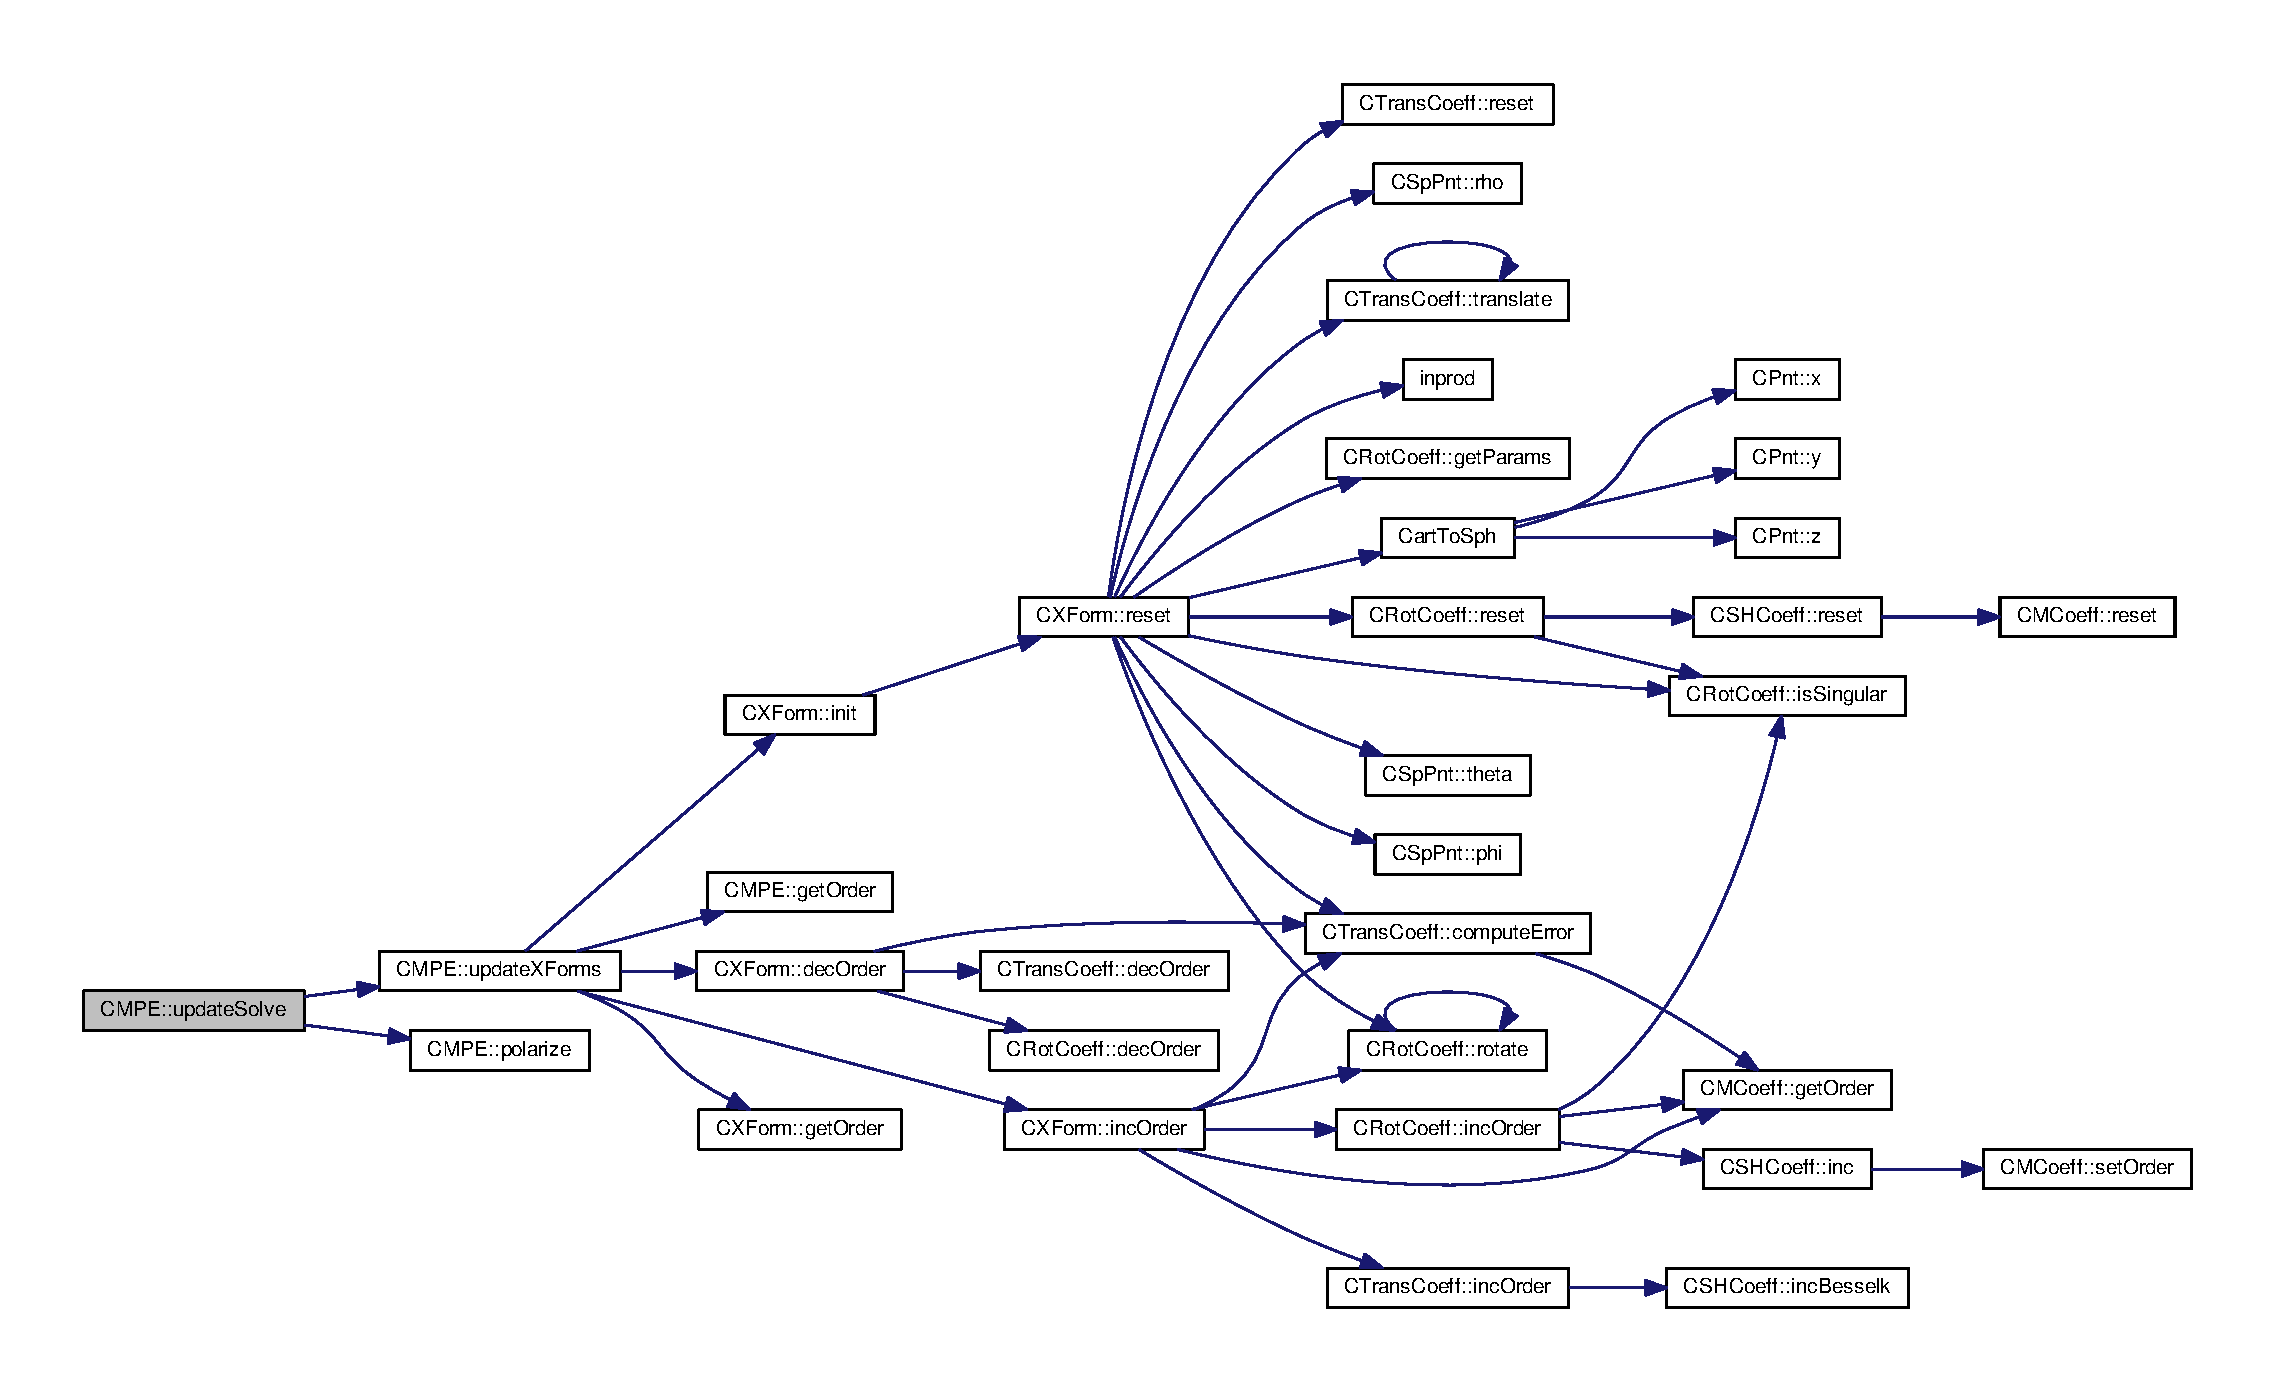
\includegraphics[width=350pt]{classCMPE_a70e20d2a606e1bae88c117b15a511e17_cgraph}
\end{center}
\end{figure}


\hypertarget{classCMPE_a65d2f19a87b451dbd84bb4b11cbfd571}{\index{C\-M\-P\-E@{C\-M\-P\-E}!update\-X\-Forms@{update\-X\-Forms}}
\index{update\-X\-Forms@{update\-X\-Forms}!CMPE@{C\-M\-P\-E}}
\subsubsection[{update\-X\-Forms}]{\setlength{\rightskip}{0pt plus 5cm}void C\-M\-P\-E\-::update\-X\-Forms (
\begin{DoxyParamCaption}
\item[{const vector$<$ {\bf C\-Pnt} $\ast$ $>$ \&}]{cen, }
\item[{vector$<$ {\bf C\-M\-P\-E} $\ast$ $>$ \&}]{mpe}
\end{DoxyParamCaption}
)\hspace{0.3cm}{\ttfamily [static]}}}\label{classCMPE_a65d2f19a87b451dbd84bb4b11cbfd571}


Function for update\-X\-Forms. 

Function of M\-P\-E class that updates transforms. 
\begin{DoxyParams}{Parameters}
{\em cen} & a vector of centers of C\-G spheres \\
\hline
{\em mpe} & a vector of M\-P\-E objects to use for polarization\\
\hline
\end{DoxyParams}
Function to update transforms. Inputs are protein centers and multipole expansions for each protein. 

Here is the call graph for this function\-:
\nopagebreak
\begin{figure}[H]
\begin{center}
\leavevmode
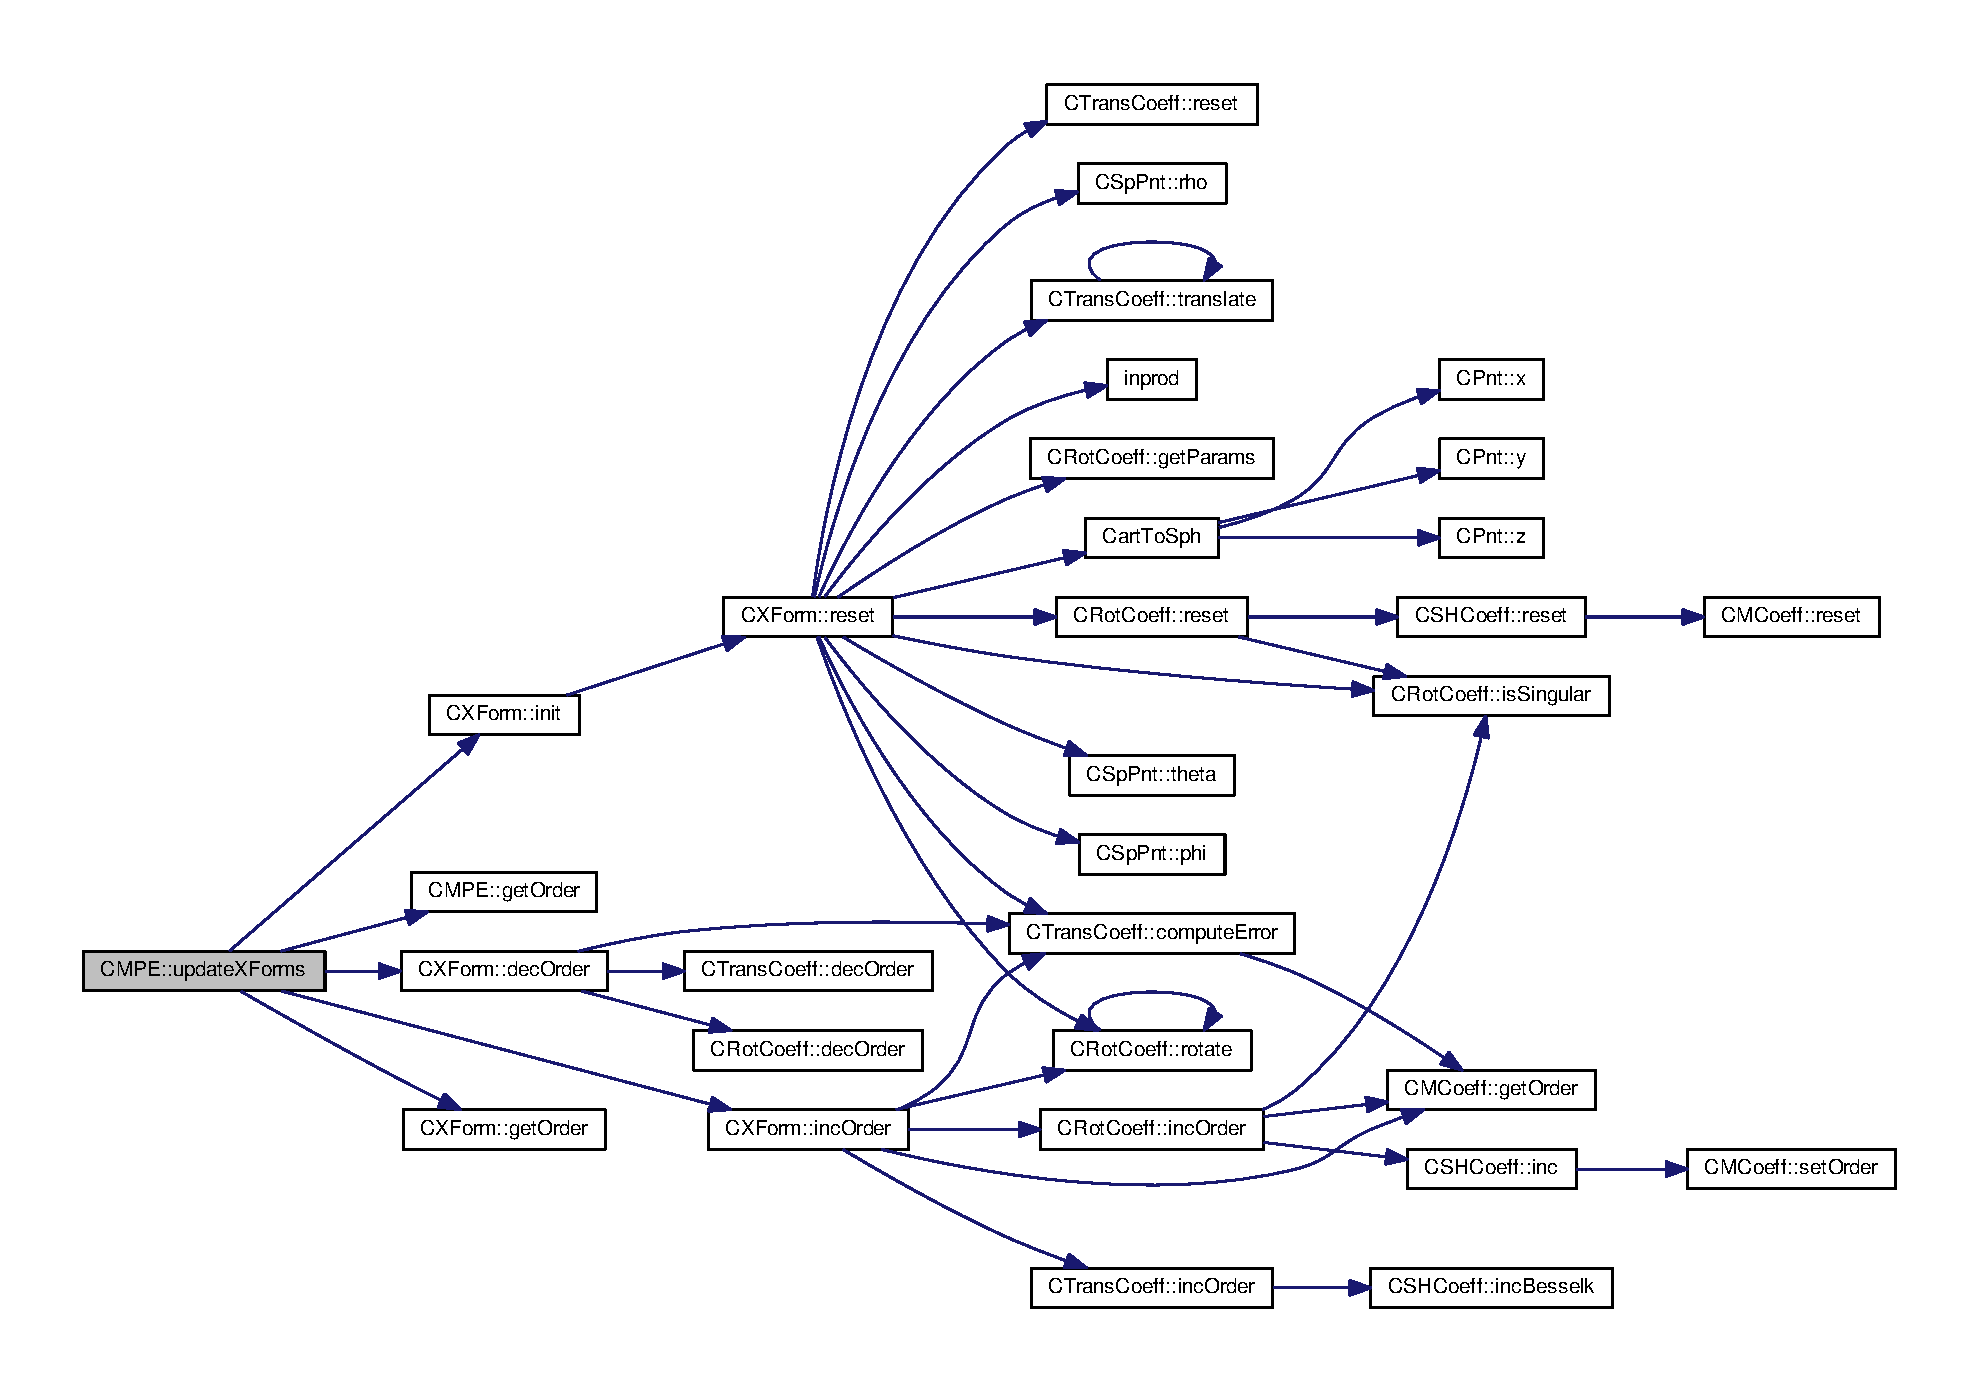
\includegraphics[width=350pt]{classCMPE_a65d2f19a87b451dbd84bb4b11cbfd571_cgraph}
\end{center}
\end{figure}




\subsection{Member Data Documentation}
\hypertarget{classCMPE_a1c612f996b0be31759020f287d3ee7cc}{\index{C\-M\-P\-E@{C\-M\-P\-E}!m\-\_\-b\-Infinite@{m\-\_\-b\-Infinite}}
\index{m\-\_\-b\-Infinite@{m\-\_\-b\-Infinite}!CMPE@{C\-M\-P\-E}}
\subsubsection[{m\-\_\-b\-Infinite}]{\setlength{\rightskip}{0pt plus 5cm}bool C\-M\-P\-E\-::m\-\_\-b\-Infinite = false\hspace{0.3cm}{\ttfamily [static]}}}\label{classCMPE_a1c612f996b0be31759020f287d3ee7cc}


Indicates whether simulation for an infinite grid is being performed. 

\hypertarget{classCMPE_adf1757fa41fec1996e7ca1c7fe6fc9e0}{\index{C\-M\-P\-E@{C\-M\-P\-E}!m\-\_\-unit@{m\-\_\-unit}}
\index{m\-\_\-unit@{m\-\_\-unit}!CMPE@{C\-M\-P\-E}}
\subsubsection[{m\-\_\-unit}]{\setlength{\rightskip}{0pt plus 5cm}int C\-M\-P\-E\-::m\-\_\-unit = 1\hspace{0.3cm}{\ttfamily [static]}}}\label{classCMPE_adf1757fa41fec1996e7ca1c7fe6fc9e0}


Unit needed for an infinite grid. Set to 1. 

\hypertarget{classCMPE_a17b9196644f13740f99675a5a0d8ef23}{\index{C\-M\-P\-E@{C\-M\-P\-E}!ngpol@{ngpol}}
\index{ngpol@{ngpol}!CMPE@{C\-M\-P\-E}}
\subsubsection[{ngpol}]{\setlength{\rightskip}{0pt plus 5cm}int C\-M\-P\-E\-::ngpol}}\label{classCMPE_a17b9196644f13740f99675a5a0d8ef23}
\hypertarget{classCMPE_afc7b0e78e954f7bb1419864a70c4d0b7}{\index{C\-M\-P\-E@{C\-M\-P\-E}!ngpol\-\_\-t@{ngpol\-\_\-t}}
\index{ngpol\-\_\-t@{ngpol\-\_\-t}!CMPE@{C\-M\-P\-E}}
\subsubsection[{ngpol\-\_\-t}]{\setlength{\rightskip}{0pt plus 5cm}{\bf R\-E\-A\-L} C\-M\-P\-E\-::ngpol\-\_\-t}}\label{classCMPE_afc7b0e78e954f7bb1419864a70c4d0b7}
\hypertarget{classCMPE_a0e97f318480ca27d2a7d608379bd2d03}{\index{C\-M\-P\-E@{C\-M\-P\-E}!tp@{tp}}
\index{tp@{tp}!CMPE@{C\-M\-P\-E}}
\subsubsection[{tp}]{\setlength{\rightskip}{0pt plus 5cm}{\bf C\-M\-P\-E} $\ast$ C\-M\-P\-E\-::tp\hspace{0.3cm}{\ttfamily [static]}}}\label{classCMPE_a0e97f318480ca27d2a7d608379bd2d03}


The documentation for this class was generated from the following files\-:\begin{DoxyCompactItemize}
\item 
\hyperlink{mpe_8h}{mpe.\-h}\item 
\hyperlink{mpe_8cpp}{mpe.\-cpp}\end{DoxyCompactItemize}

\hypertarget{classCPDB}{\section{C\-P\-D\-B Class Reference}
\label{classCPDB}\index{C\-P\-D\-B@{C\-P\-D\-B}}
}


The P\-D\-B class.  




{\ttfamily \#include $<$pdb.\-h$>$}

\subsection*{Static Public Member Functions}
\begin{DoxyCompactItemize}
\item 
static void \hyperlink{classCPDB_a3033b818c15dea1b6df7c3b354a8d044}{load\-From\-P\-D\-B} (const char $\ast$fname, vector$<$ \hyperlink{classAA}{A\-A} $>$ \&aas)
\begin{DoxyCompactList}\small\item\em The P\-D\-B function load\-From\-P\-D\-B. \end{DoxyCompactList}\item 
static void \hyperlink{classCPDB_ab30dfa8082d957c7008d2e4a2c56273b}{write\-To\-P\-D\-B} (const char $\ast$fname, const vector$<$ \hyperlink{classAA}{A\-A} $>$ \&aas)
\begin{DoxyCompactList}\small\item\em The P\-D\-B function write\-To\-P\-D\-B. \end{DoxyCompactList}\item 
static void \hyperlink{classCPDB_a1c4247e99968afb8266c6cf85d537de6}{write\-Line} (ostream \&fout, int index, const char $\ast$chainid, const \hyperlink{classCAtom}{C\-Atom} \&atom, const \hyperlink{classCQuat}{C\-Quat} \&rot, const \hyperlink{classCPnt}{C\-Pnt} \&trans)
\begin{DoxyCompactList}\small\item\em The P\-D\-B function write\-Line. \end{DoxyCompactList}\item 
static \hyperlink{classCAtom}{C\-Atom} \hyperlink{classCPDB_acdc2ba2ed5bb4dc8701577e29c0f4bf9}{readline} (const char $\ast$buf)
\begin{DoxyCompactList}\small\item\em The P\-D\-B function read\-Line. \end{DoxyCompactList}\end{DoxyCompactItemize}


\subsection{Detailed Description}
The P\-D\-B class. 

The class that contains all details for a P\-D\-B object 

\subsection{Member Function Documentation}
\hypertarget{classCPDB_a3033b818c15dea1b6df7c3b354a8d044}{\index{C\-P\-D\-B@{C\-P\-D\-B}!load\-From\-P\-D\-B@{load\-From\-P\-D\-B}}
\index{load\-From\-P\-D\-B@{load\-From\-P\-D\-B}!CPDB@{C\-P\-D\-B}}
\subsubsection[{load\-From\-P\-D\-B}]{\setlength{\rightskip}{0pt plus 5cm}void C\-P\-D\-B\-::load\-From\-P\-D\-B (
\begin{DoxyParamCaption}
\item[{const char $\ast$}]{fname, }
\item[{vector$<$ {\bf A\-A} $>$ \&}]{aas}
\end{DoxyParamCaption}
)\hspace{0.3cm}{\ttfamily [static]}}}\label{classCPDB_a3033b818c15dea1b6df7c3b354a8d044}


The P\-D\-B function load\-From\-P\-D\-B. 

The function that opens a P\-D\-B and reads in the atoms in it, storing each in their respective amino acid groups 
\begin{DoxyParams}{Parameters}
{\em fname} & a character string of the filename handle \\
\hline
{\em a} & vector of amino acids to store information from P\-D\-B\\
\hline
\end{DoxyParams}
load\-From\-P\-D\-B Inputs\-: pdb filename for protein, empty vector for amino acid seq 

Here is the call graph for this function\-:
\nopagebreak
\begin{figure}[H]
\begin{center}
\leavevmode
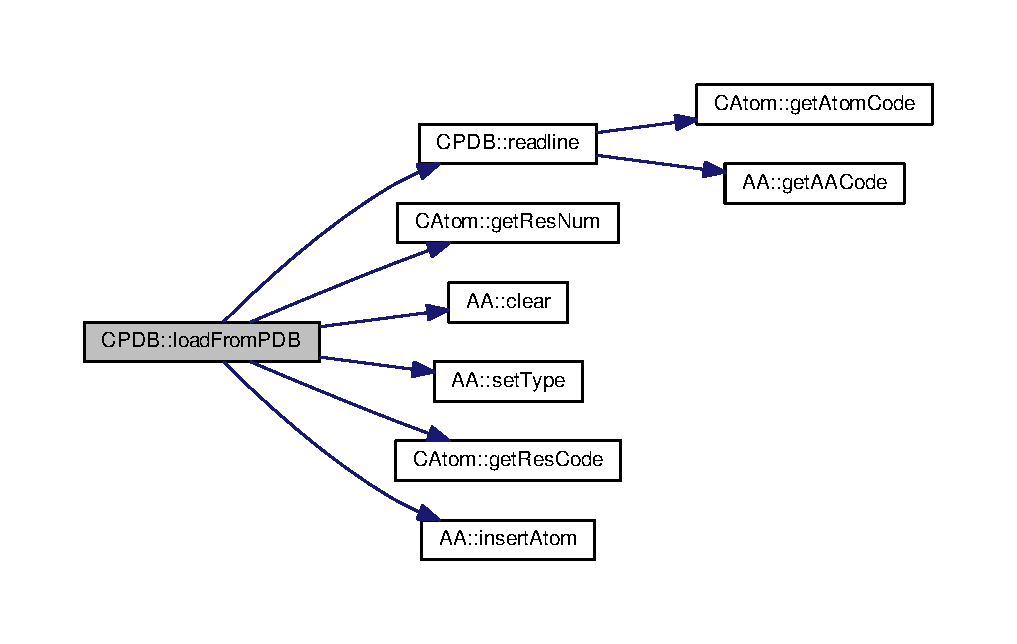
\includegraphics[width=350pt]{classCPDB_a3033b818c15dea1b6df7c3b354a8d044_cgraph}
\end{center}
\end{figure}


\hypertarget{classCPDB_acdc2ba2ed5bb4dc8701577e29c0f4bf9}{\index{C\-P\-D\-B@{C\-P\-D\-B}!readline@{readline}}
\index{readline@{readline}!CPDB@{C\-P\-D\-B}}
\subsubsection[{readline}]{\setlength{\rightskip}{0pt plus 5cm}{\bf C\-Atom} C\-P\-D\-B\-::readline (
\begin{DoxyParamCaption}
\item[{const char $\ast$}]{buf}
\end{DoxyParamCaption}
)\hspace{0.3cm}{\ttfamily [static]}}}\label{classCPDB_acdc2ba2ed5bb4dc8701577e29c0f4bf9}


The P\-D\-B function read\-Line. 

The function called by load\-From\-P\-D\-B to read in a line and store as a \hyperlink{classCAtom}{C\-Atom} class object 
\begin{DoxyParams}{Parameters}
{\em buf} & a string from the P\-D\-B file \\
\hline
\end{DoxyParams}
\begin{DoxyReturn}{Returns}
\hyperlink{classCAtom}{C\-Atom} object of the atom information contained on the line
\end{DoxyReturn}
read\-Line\-: read a line from a pdb file to obtain information about an atom 

Here is the call graph for this function\-:
\nopagebreak
\begin{figure}[H]
\begin{center}
\leavevmode
\includegraphics[width=316pt]{classCPDB_acdc2ba2ed5bb4dc8701577e29c0f4bf9_cgraph}
\end{center}
\end{figure}


\hypertarget{classCPDB_a1c4247e99968afb8266c6cf85d537de6}{\index{C\-P\-D\-B@{C\-P\-D\-B}!write\-Line@{write\-Line}}
\index{write\-Line@{write\-Line}!CPDB@{C\-P\-D\-B}}
\subsubsection[{write\-Line}]{\setlength{\rightskip}{0pt plus 5cm}void C\-P\-D\-B\-::write\-Line (
\begin{DoxyParamCaption}
\item[{ostream \&}]{fout, }
\item[{int}]{index, }
\item[{const char $\ast$}]{chainid, }
\item[{const {\bf C\-Atom} \&}]{atom, }
\item[{const {\bf C\-Quat} \&}]{rot, }
\item[{const {\bf C\-Pnt} \&}]{trans}
\end{DoxyParamCaption}
)\hspace{0.3cm}{\ttfamily [static]}}}\label{classCPDB_a1c4247e99968afb8266c6cf85d537de6}


The P\-D\-B function write\-Line. 

The function called by write\-To\-P\-D\-B to write out each line 
\begin{DoxyParams}{Parameters}
{\em fout} & a character string of the filename handle \\
\hline
{\em int} & an index of the atom number \\
\hline
{\em chain\-Id} & a character string of the chain I\-D \\
\hline
{\em atom} & a \hyperlink{classCAtom}{C\-Atom} object of the atom to print \\
\hline
{\em rot} & a \hyperlink{classCQuat}{C\-Quat} object of the atom's orientation \\
\hline
{\em trans} & a \hyperlink{classCPnt}{C\-Pnt} object of the atoms translation\\
\hline
\end{DoxyParams}
The function called by write\-To\-P\-D\-B to write out each line 

Here is the call graph for this function\-:
\nopagebreak
\begin{figure}[H]
\begin{center}
\leavevmode
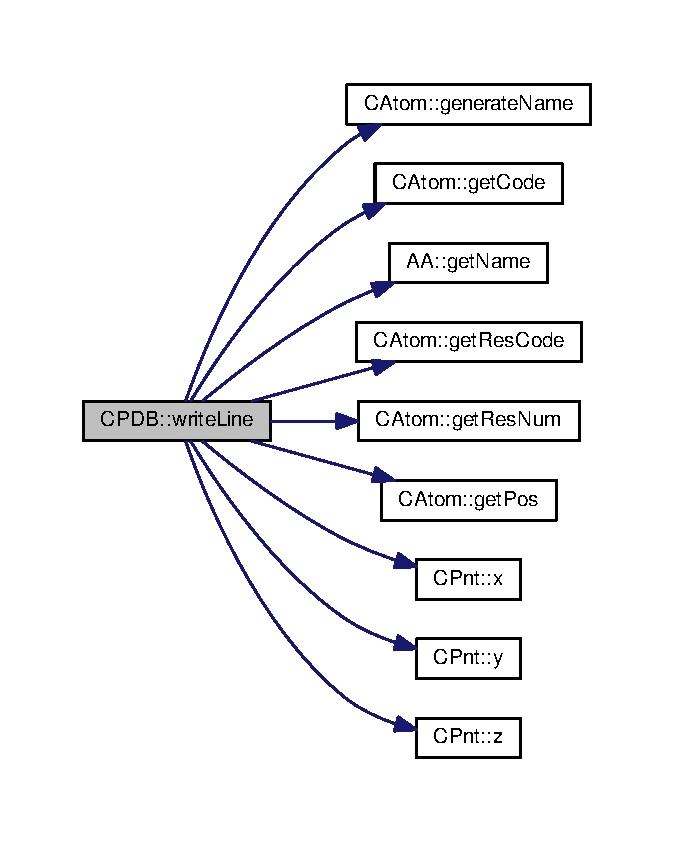
\includegraphics[width=324pt]{classCPDB_a1c4247e99968afb8266c6cf85d537de6_cgraph}
\end{center}
\end{figure}


\hypertarget{classCPDB_ab30dfa8082d957c7008d2e4a2c56273b}{\index{C\-P\-D\-B@{C\-P\-D\-B}!write\-To\-P\-D\-B@{write\-To\-P\-D\-B}}
\index{write\-To\-P\-D\-B@{write\-To\-P\-D\-B}!CPDB@{C\-P\-D\-B}}
\subsubsection[{write\-To\-P\-D\-B}]{\setlength{\rightskip}{0pt plus 5cm}void C\-P\-D\-B\-::write\-To\-P\-D\-B (
\begin{DoxyParamCaption}
\item[{const char $\ast$}]{fname, }
\item[{const vector$<$ {\bf A\-A} $>$ \&}]{aas}
\end{DoxyParamCaption}
)\hspace{0.3cm}{\ttfamily [static]}}}\label{classCPDB_ab30dfa8082d957c7008d2e4a2c56273b}


The P\-D\-B function write\-To\-P\-D\-B. 

The function that writes out a group of amino acids to a P\-D\-B 
\begin{DoxyParams}{Parameters}
{\em fname} & a character string of the filename handle \\
\hline
{\em a} & vector of amino acids to print to P\-D\-B\\
\hline
\end{DoxyParams}
The function that writes out a group of amino acids to a P\-D\-B 

The documentation for this class was generated from the following files\-:\begin{DoxyCompactItemize}
\item 
\hyperlink{pdb_8h}{pdb.\-h}\item 
\hyperlink{pdb_8cpp}{pdb.\-cpp}\end{DoxyCompactItemize}

\hypertarget{classCPnt}{\section{C\-Pnt Class Reference}
\label{classCPnt}\index{C\-Pnt@{C\-Pnt}}
}


The cartesian coordinate class.  




{\ttfamily \#include $<$util.\-h$>$}

\subsection*{Public Member Functions}
\begin{DoxyCompactItemize}
\item 
\hyperlink{classCPnt_a6792dcfc8b95c18c03bda5a6dde7765a}{C\-Pnt} ()
\item 
\hyperlink{classCPnt_a91907d073421cdf75000d27f982f058b}{C\-Pnt} (\hyperlink{util_8h_a5821460e95a0800cf9f24c38915cbbde}{R\-E\-A\-L} x\-\_\-, \hyperlink{util_8h_a5821460e95a0800cf9f24c38915cbbde}{R\-E\-A\-L} y\-\_\-, \hyperlink{util_8h_a5821460e95a0800cf9f24c38915cbbde}{R\-E\-A\-L} z\-\_\-)
\item 
\hyperlink{classCPnt_aca4d8d7044e71700128b497cfcc4f1d8}{C\-Pnt} (const \hyperlink{classCPnt}{C\-Pnt} \&p)
\item 
const \hyperlink{classCPnt}{C\-Pnt} \& \hyperlink{classCPnt_abd18aa7c83ac70f5e73847a8cd154e9d}{operator=} (const \hyperlink{classCPnt}{C\-Pnt} \&c)
\item 
void \hyperlink{classCPnt_a619a71665a5a40fddbc8e6c6a6b450cc}{zero} ()
\item 
\hyperlink{util_8h_a5821460e95a0800cf9f24c38915cbbde}{R\-E\-A\-L} \hyperlink{classCPnt_ac4dcf209c35c4ef0c119cd59fbddd18f}{normsq} () const 
\item 
\hyperlink{util_8h_a5821460e95a0800cf9f24c38915cbbde}{R\-E\-A\-L} \hyperlink{classCPnt_ab92f2e6cc3891ff6a00eddb483b854ab}{norm} () const 
\item 
const \hyperlink{classCPnt}{C\-Pnt} \& \hyperlink{classCPnt_a79e4515e6479905942ce4b48990943f0}{normalize} ()
\item 
\hyperlink{classCPnt}{C\-Pnt} \hyperlink{classCPnt_a59899074de56c4ad55583fc58d48ea0a}{normalize} () const 
\item 
void \hyperlink{classCPnt_ab9aa57d527e60e0ba46fd44ee515ebb0}{operator+=} (const \hyperlink{classCPnt}{C\-Pnt} \&p)
\item 
void \hyperlink{classCPnt_aad46f39ec4811f1f7c39b33b0ef55f42}{operator-\/=} (const \hyperlink{classCPnt}{C\-Pnt} \&p)
\item 
void \hyperlink{classCPnt_a30b6c20eb5777d321202db9006fe5dc0}{operator$\ast$=} (\hyperlink{util_8h_a5821460e95a0800cf9f24c38915cbbde}{R\-E\-A\-L} s)
\item 
void \hyperlink{classCPnt_a5ef5437f322871129c1398ab5f5e8764}{operator/=} (\hyperlink{util_8h_a5821460e95a0800cf9f24c38915cbbde}{R\-E\-A\-L} s)
\item 
const \hyperlink{util_8h_a5821460e95a0800cf9f24c38915cbbde}{R\-E\-A\-L} \hyperlink{classCPnt_a5867d45fc05ae371116367067eb23f48}{x} () const 
\item 
const \hyperlink{util_8h_a5821460e95a0800cf9f24c38915cbbde}{R\-E\-A\-L} \hyperlink{classCPnt_ac9283f60e70f312ee1784de6c6ea5aec}{y} () const 
\item 
const \hyperlink{util_8h_a5821460e95a0800cf9f24c38915cbbde}{R\-E\-A\-L} \hyperlink{classCPnt_a37d139ebe50234ab753472b896c7d17c}{z} () const 
\item 
\hyperlink{util_8h_a5821460e95a0800cf9f24c38915cbbde}{R\-E\-A\-L} \& \hyperlink{classCPnt_ac7a36844c1474f7d89f27c5ab3e083b2}{x} ()
\item 
\hyperlink{util_8h_a5821460e95a0800cf9f24c38915cbbde}{R\-E\-A\-L} \& \hyperlink{classCPnt_afa7c12f6ae5daf81779e92692c5024ce}{y} ()
\item 
\hyperlink{util_8h_a5821460e95a0800cf9f24c38915cbbde}{R\-E\-A\-L} \& \hyperlink{classCPnt_a6a5263d7b30cc4776336ac9598416757}{z} ()
\end{DoxyCompactItemize}
\subsection*{Friends}
\begin{DoxyCompactItemize}
\item 
\hyperlink{classCPnt}{C\-Pnt} \hyperlink{classCPnt_a793e034bed9900c45412db255d708e84}{operator+} (const \hyperlink{classCPnt}{C\-Pnt} \&p1, const \hyperlink{classCPnt}{C\-Pnt} \&p2)
\begin{DoxyCompactList}\small\item\em \hyperlink{classCPnt}{C\-Pnt} +. \end{DoxyCompactList}\item 
\hyperlink{classCPnt}{C\-Pnt} \hyperlink{classCPnt_a7b0ef59814c5c3ae6a9165df62ab8598}{operator-\/} (const \hyperlink{classCPnt}{C\-Pnt} \&p1, const \hyperlink{classCPnt}{C\-Pnt} \&p2)
\begin{DoxyCompactList}\small\item\em \hyperlink{classCPnt}{C\-Pnt} -\/. \end{DoxyCompactList}\item 
\hyperlink{classCPnt}{C\-Pnt} \hyperlink{classCPnt_ab4553c75d2ac17d0539471baeb0c0237}{cross} (const \hyperlink{classCPnt}{C\-Pnt} \&p1, const \hyperlink{classCPnt}{C\-Pnt} \&p2)
\begin{DoxyCompactList}\small\item\em \hyperlink{classCPnt}{C\-Pnt} cross. \end{DoxyCompactList}\item 
\hyperlink{classCPnt}{C\-Pnt} \hyperlink{classCPnt_a6bf4a1152989f36cdb084e617a81214b}{operator$\ast$} (\hyperlink{util_8h_a5821460e95a0800cf9f24c38915cbbde}{R\-E\-A\-L} c, const \hyperlink{classCPnt}{C\-Pnt} \&p1)
\begin{DoxyCompactList}\small\item\em \hyperlink{classCPnt}{C\-Pnt} $\ast$ scalar. \end{DoxyCompactList}\item 
\hyperlink{classCPnt}{C\-Pnt} \hyperlink{classCPnt_a77ba614aeb115f5ab29247677cc4fa05}{operator-\/} (const \hyperlink{classCPnt}{C\-Pnt} \&p)
\begin{DoxyCompactList}\small\item\em \hyperlink{classCPnt}{C\-Pnt} -\/. \end{DoxyCompactList}\item 
ostream \& \hyperlink{classCPnt_a5d9fde839f5480f04e4b64a9621e3370}{operator$<$$<$} (ostream \&out, const \hyperlink{classCPnt}{C\-Pnt} \&p)
\begin{DoxyCompactList}\small\item\em \hyperlink{classCPnt}{C\-Pnt} $<$$<$. \end{DoxyCompactList}\item 
\hyperlink{classCPnt}{C\-Pnt} \hyperlink{classCPnt_af8b263bb80bb3a76271a7f57d5057df3}{Sph\-To\-Cart} (const \hyperlink{classCSpPnt}{C\-Sp\-Pnt} \&s)
\begin{DoxyCompactList}\small\item\em \hyperlink{classCSpPnt}{C\-Sp\-Pnt} Sph\-To\-Cart. \end{DoxyCompactList}\item 
\hyperlink{classCSpPnt}{C\-Sp\-Pnt} \hyperlink{classCPnt_ad05fbf75e7550a927bc817f97115f2fc}{Cart\-To\-Sph} (const \hyperlink{classCPnt}{C\-Pnt} \&c)
\begin{DoxyCompactList}\small\item\em \hyperlink{classCSpPnt}{C\-Sp\-Pnt} Cart\-To\-Sph. \end{DoxyCompactList}\item 
\hyperlink{util_8h_a5821460e95a0800cf9f24c38915cbbde}{R\-E\-A\-L} \hyperlink{classCPnt_ac25278586b4a84caf4098513d812d60b}{torsion} (const \hyperlink{classCPnt}{C\-Pnt} \&p1, const \hyperlink{classCPnt}{C\-Pnt} \&p2, const \hyperlink{classCPnt}{C\-Pnt} \&p3, const \hyperlink{classCPnt}{C\-Pnt} \&p4)
\begin{DoxyCompactList}\small\item\em \hyperlink{classCPnt}{C\-Pnt} torsion. \end{DoxyCompactList}\item 
\hyperlink{util_8h_a5821460e95a0800cf9f24c38915cbbde}{R\-E\-A\-L} \hyperlink{classCPnt_a774fe41d28888a078993d8d3384c34d8}{torsion} (const \hyperlink{classCPnt}{C\-Pnt} \&v1, const \hyperlink{classCPnt}{C\-Pnt} \&v2, const \hyperlink{classCPnt}{C\-Pnt} \&v3)
\begin{DoxyCompactList}\small\item\em \hyperlink{classCPnt}{C\-Pnt} torsion. \end{DoxyCompactList}\end{DoxyCompactItemize}


\subsection{Detailed Description}
The cartesian coordinate class. 

The class that contains all details for a cartesian coordinate object 

\subsection{Constructor \& Destructor Documentation}
\hypertarget{classCPnt_a6792dcfc8b95c18c03bda5a6dde7765a}{\index{C\-Pnt@{C\-Pnt}!C\-Pnt@{C\-Pnt}}
\index{C\-Pnt@{C\-Pnt}!CPnt@{C\-Pnt}}
\subsubsection[{C\-Pnt}]{\setlength{\rightskip}{0pt plus 5cm}C\-Pnt\-::\-C\-Pnt (
\begin{DoxyParamCaption}
{}
\end{DoxyParamCaption}
)\hspace{0.3cm}{\ttfamily [inline]}}}\label{classCPnt_a6792dcfc8b95c18c03bda5a6dde7765a}
\hypertarget{classCPnt_a91907d073421cdf75000d27f982f058b}{\index{C\-Pnt@{C\-Pnt}!C\-Pnt@{C\-Pnt}}
\index{C\-Pnt@{C\-Pnt}!CPnt@{C\-Pnt}}
\subsubsection[{C\-Pnt}]{\setlength{\rightskip}{0pt plus 5cm}C\-Pnt\-::\-C\-Pnt (
\begin{DoxyParamCaption}
\item[{{\bf R\-E\-A\-L}}]{x\-\_\-, }
\item[{{\bf R\-E\-A\-L}}]{y\-\_\-, }
\item[{{\bf R\-E\-A\-L}}]{z\-\_\-}
\end{DoxyParamCaption}
)\hspace{0.3cm}{\ttfamily [inline]}}}\label{classCPnt_a91907d073421cdf75000d27f982f058b}
\hypertarget{classCPnt_aca4d8d7044e71700128b497cfcc4f1d8}{\index{C\-Pnt@{C\-Pnt}!C\-Pnt@{C\-Pnt}}
\index{C\-Pnt@{C\-Pnt}!CPnt@{C\-Pnt}}
\subsubsection[{C\-Pnt}]{\setlength{\rightskip}{0pt plus 5cm}C\-Pnt\-::\-C\-Pnt (
\begin{DoxyParamCaption}
\item[{const {\bf C\-Pnt} \&}]{p}
\end{DoxyParamCaption}
)\hspace{0.3cm}{\ttfamily [inline]}}}\label{classCPnt_aca4d8d7044e71700128b497cfcc4f1d8}


\subsection{Member Function Documentation}
\hypertarget{classCPnt_ab92f2e6cc3891ff6a00eddb483b854ab}{\index{C\-Pnt@{C\-Pnt}!norm@{norm}}
\index{norm@{norm}!CPnt@{C\-Pnt}}
\subsubsection[{norm}]{\setlength{\rightskip}{0pt plus 5cm}{\bf R\-E\-A\-L} C\-Pnt\-::norm (
\begin{DoxyParamCaption}
{}
\end{DoxyParamCaption}
) const\hspace{0.3cm}{\ttfamily [inline]}}}\label{classCPnt_ab92f2e6cc3891ff6a00eddb483b854ab}
\hypertarget{classCPnt_a79e4515e6479905942ce4b48990943f0}{\index{C\-Pnt@{C\-Pnt}!normalize@{normalize}}
\index{normalize@{normalize}!CPnt@{C\-Pnt}}
\subsubsection[{normalize}]{\setlength{\rightskip}{0pt plus 5cm}const {\bf C\-Pnt}\& C\-Pnt\-::normalize (
\begin{DoxyParamCaption}
{}
\end{DoxyParamCaption}
)\hspace{0.3cm}{\ttfamily [inline]}}}\label{classCPnt_a79e4515e6479905942ce4b48990943f0}
\hypertarget{classCPnt_a59899074de56c4ad55583fc58d48ea0a}{\index{C\-Pnt@{C\-Pnt}!normalize@{normalize}}
\index{normalize@{normalize}!CPnt@{C\-Pnt}}
\subsubsection[{normalize}]{\setlength{\rightskip}{0pt plus 5cm}{\bf C\-Pnt} C\-Pnt\-::normalize (
\begin{DoxyParamCaption}
{}
\end{DoxyParamCaption}
) const\hspace{0.3cm}{\ttfamily [inline]}}}\label{classCPnt_a59899074de56c4ad55583fc58d48ea0a}
\hypertarget{classCPnt_ac4dcf209c35c4ef0c119cd59fbddd18f}{\index{C\-Pnt@{C\-Pnt}!normsq@{normsq}}
\index{normsq@{normsq}!CPnt@{C\-Pnt}}
\subsubsection[{normsq}]{\setlength{\rightskip}{0pt plus 5cm}{\bf R\-E\-A\-L} C\-Pnt\-::normsq (
\begin{DoxyParamCaption}
{}
\end{DoxyParamCaption}
) const\hspace{0.3cm}{\ttfamily [inline]}}}\label{classCPnt_ac4dcf209c35c4ef0c119cd59fbddd18f}


Here is the call graph for this function\-:
\nopagebreak
\begin{figure}[H]
\begin{center}
\leavevmode
\includegraphics[width=310pt]{classCPnt_ac4dcf209c35c4ef0c119cd59fbddd18f_cgraph}
\end{center}
\end{figure}


\hypertarget{classCPnt_a30b6c20eb5777d321202db9006fe5dc0}{\index{C\-Pnt@{C\-Pnt}!operator$\ast$=@{operator$\ast$=}}
\index{operator$\ast$=@{operator$\ast$=}!CPnt@{C\-Pnt}}
\subsubsection[{operator$\ast$=}]{\setlength{\rightskip}{0pt plus 5cm}void C\-Pnt\-::operator$\ast$= (
\begin{DoxyParamCaption}
\item[{{\bf R\-E\-A\-L}}]{s}
\end{DoxyParamCaption}
)\hspace{0.3cm}{\ttfamily [inline]}}}\label{classCPnt_a30b6c20eb5777d321202db9006fe5dc0}
\hypertarget{classCPnt_ab9aa57d527e60e0ba46fd44ee515ebb0}{\index{C\-Pnt@{C\-Pnt}!operator+=@{operator+=}}
\index{operator+=@{operator+=}!CPnt@{C\-Pnt}}
\subsubsection[{operator+=}]{\setlength{\rightskip}{0pt plus 5cm}void C\-Pnt\-::operator+= (
\begin{DoxyParamCaption}
\item[{const {\bf C\-Pnt} \&}]{p}
\end{DoxyParamCaption}
)\hspace{0.3cm}{\ttfamily [inline]}}}\label{classCPnt_ab9aa57d527e60e0ba46fd44ee515ebb0}


Here is the call graph for this function\-:\nopagebreak
\begin{figure}[H]
\begin{center}
\leavevmode
\includegraphics[width=258pt]{classCPnt_ab9aa57d527e60e0ba46fd44ee515ebb0_cgraph}
\end{center}
\end{figure}


\hypertarget{classCPnt_aad46f39ec4811f1f7c39b33b0ef55f42}{\index{C\-Pnt@{C\-Pnt}!operator-\/=@{operator-\/=}}
\index{operator-\/=@{operator-\/=}!CPnt@{C\-Pnt}}
\subsubsection[{operator-\/=}]{\setlength{\rightskip}{0pt plus 5cm}void C\-Pnt\-::operator-\/= (
\begin{DoxyParamCaption}
\item[{const {\bf C\-Pnt} \&}]{p}
\end{DoxyParamCaption}
)\hspace{0.3cm}{\ttfamily [inline]}}}\label{classCPnt_aad46f39ec4811f1f7c39b33b0ef55f42}


Here is the call graph for this function\-:\nopagebreak
\begin{figure}[H]
\begin{center}
\leavevmode
\includegraphics[width=256pt]{classCPnt_aad46f39ec4811f1f7c39b33b0ef55f42_cgraph}
\end{center}
\end{figure}


\hypertarget{classCPnt_a5ef5437f322871129c1398ab5f5e8764}{\index{C\-Pnt@{C\-Pnt}!operator/=@{operator/=}}
\index{operator/=@{operator/=}!CPnt@{C\-Pnt}}
\subsubsection[{operator/=}]{\setlength{\rightskip}{0pt plus 5cm}void C\-Pnt\-::operator/= (
\begin{DoxyParamCaption}
\item[{{\bf R\-E\-A\-L}}]{s}
\end{DoxyParamCaption}
)\hspace{0.3cm}{\ttfamily [inline]}}}\label{classCPnt_a5ef5437f322871129c1398ab5f5e8764}
\hypertarget{classCPnt_abd18aa7c83ac70f5e73847a8cd154e9d}{\index{C\-Pnt@{C\-Pnt}!operator=@{operator=}}
\index{operator=@{operator=}!CPnt@{C\-Pnt}}
\subsubsection[{operator=}]{\setlength{\rightskip}{0pt plus 5cm}const {\bf C\-Pnt}\& C\-Pnt\-::operator= (
\begin{DoxyParamCaption}
\item[{const {\bf C\-Pnt} \&}]{c}
\end{DoxyParamCaption}
)\hspace{0.3cm}{\ttfamily [inline]}}}\label{classCPnt_abd18aa7c83ac70f5e73847a8cd154e9d}


Here is the call graph for this function\-:\nopagebreak
\begin{figure}[H]
\begin{center}
\leavevmode
\includegraphics[width=252pt]{classCPnt_abd18aa7c83ac70f5e73847a8cd154e9d_cgraph}
\end{center}
\end{figure}


\hypertarget{classCPnt_a5867d45fc05ae371116367067eb23f48}{\index{C\-Pnt@{C\-Pnt}!x@{x}}
\index{x@{x}!CPnt@{C\-Pnt}}
\subsubsection[{x}]{\setlength{\rightskip}{0pt plus 5cm}const {\bf R\-E\-A\-L} C\-Pnt\-::x (
\begin{DoxyParamCaption}
{}
\end{DoxyParamCaption}
) const\hspace{0.3cm}{\ttfamily [inline]}}}\label{classCPnt_a5867d45fc05ae371116367067eb23f48}
\hypertarget{classCPnt_ac7a36844c1474f7d89f27c5ab3e083b2}{\index{C\-Pnt@{C\-Pnt}!x@{x}}
\index{x@{x}!CPnt@{C\-Pnt}}
\subsubsection[{x}]{\setlength{\rightskip}{0pt plus 5cm}{\bf R\-E\-A\-L}\& C\-Pnt\-::x (
\begin{DoxyParamCaption}
{}
\end{DoxyParamCaption}
)\hspace{0.3cm}{\ttfamily [inline]}}}\label{classCPnt_ac7a36844c1474f7d89f27c5ab3e083b2}
\hypertarget{classCPnt_ac9283f60e70f312ee1784de6c6ea5aec}{\index{C\-Pnt@{C\-Pnt}!y@{y}}
\index{y@{y}!CPnt@{C\-Pnt}}
\subsubsection[{y}]{\setlength{\rightskip}{0pt plus 5cm}const {\bf R\-E\-A\-L} C\-Pnt\-::y (
\begin{DoxyParamCaption}
{}
\end{DoxyParamCaption}
) const\hspace{0.3cm}{\ttfamily [inline]}}}\label{classCPnt_ac9283f60e70f312ee1784de6c6ea5aec}
\hypertarget{classCPnt_afa7c12f6ae5daf81779e92692c5024ce}{\index{C\-Pnt@{C\-Pnt}!y@{y}}
\index{y@{y}!CPnt@{C\-Pnt}}
\subsubsection[{y}]{\setlength{\rightskip}{0pt plus 5cm}{\bf R\-E\-A\-L}\& C\-Pnt\-::y (
\begin{DoxyParamCaption}
{}
\end{DoxyParamCaption}
)\hspace{0.3cm}{\ttfamily [inline]}}}\label{classCPnt_afa7c12f6ae5daf81779e92692c5024ce}
\hypertarget{classCPnt_a37d139ebe50234ab753472b896c7d17c}{\index{C\-Pnt@{C\-Pnt}!z@{z}}
\index{z@{z}!CPnt@{C\-Pnt}}
\subsubsection[{z}]{\setlength{\rightskip}{0pt plus 5cm}const {\bf R\-E\-A\-L} C\-Pnt\-::z (
\begin{DoxyParamCaption}
{}
\end{DoxyParamCaption}
) const\hspace{0.3cm}{\ttfamily [inline]}}}\label{classCPnt_a37d139ebe50234ab753472b896c7d17c}
\hypertarget{classCPnt_a6a5263d7b30cc4776336ac9598416757}{\index{C\-Pnt@{C\-Pnt}!z@{z}}
\index{z@{z}!CPnt@{C\-Pnt}}
\subsubsection[{z}]{\setlength{\rightskip}{0pt plus 5cm}{\bf R\-E\-A\-L}\& C\-Pnt\-::z (
\begin{DoxyParamCaption}
{}
\end{DoxyParamCaption}
)\hspace{0.3cm}{\ttfamily [inline]}}}\label{classCPnt_a6a5263d7b30cc4776336ac9598416757}
\hypertarget{classCPnt_a619a71665a5a40fddbc8e6c6a6b450cc}{\index{C\-Pnt@{C\-Pnt}!zero@{zero}}
\index{zero@{zero}!CPnt@{C\-Pnt}}
\subsubsection[{zero}]{\setlength{\rightskip}{0pt plus 5cm}void C\-Pnt\-::zero (
\begin{DoxyParamCaption}
{}
\end{DoxyParamCaption}
)\hspace{0.3cm}{\ttfamily [inline]}}}\label{classCPnt_a619a71665a5a40fddbc8e6c6a6b450cc}


\subsection{Friends And Related Function Documentation}
\hypertarget{classCPnt_ad05fbf75e7550a927bc817f97115f2fc}{\index{C\-Pnt@{C\-Pnt}!Cart\-To\-Sph@{Cart\-To\-Sph}}
\index{Cart\-To\-Sph@{Cart\-To\-Sph}!CPnt@{C\-Pnt}}
\subsubsection[{Cart\-To\-Sph}]{\setlength{\rightskip}{0pt plus 5cm}{\bf C\-Sp\-Pnt} Cart\-To\-Sph (
\begin{DoxyParamCaption}
\item[{const {\bf C\-Pnt} \&}]{c}
\end{DoxyParamCaption}
)\hspace{0.3cm}{\ttfamily [friend]}}}\label{classCPnt_ad05fbf75e7550a927bc817f97115f2fc}


\hyperlink{classCSpPnt}{C\-Sp\-Pnt} Cart\-To\-Sph. 

Converting from cartesian to spherical coordinates \hypertarget{classCPnt_ab4553c75d2ac17d0539471baeb0c0237}{\index{C\-Pnt@{C\-Pnt}!cross@{cross}}
\index{cross@{cross}!CPnt@{C\-Pnt}}
\subsubsection[{cross}]{\setlength{\rightskip}{0pt plus 5cm}{\bf C\-Pnt} cross (
\begin{DoxyParamCaption}
\item[{const {\bf C\-Pnt} \&}]{p1, }
\item[{const {\bf C\-Pnt} \&}]{p2}
\end{DoxyParamCaption}
)\hspace{0.3cm}{\ttfamily [friend]}}}\label{classCPnt_ab4553c75d2ac17d0539471baeb0c0237}


\hyperlink{classCPnt}{C\-Pnt} cross. 

Cross product of two vectors \hypertarget{classCPnt_a6bf4a1152989f36cdb084e617a81214b}{\index{C\-Pnt@{C\-Pnt}!operator$\ast$@{operator$\ast$}}
\index{operator$\ast$@{operator$\ast$}!CPnt@{C\-Pnt}}
\subsubsection[{operator$\ast$}]{\setlength{\rightskip}{0pt plus 5cm}{\bf C\-Pnt} operator$\ast$ (
\begin{DoxyParamCaption}
\item[{{\bf R\-E\-A\-L}}]{c, }
\item[{const {\bf C\-Pnt} \&}]{p1}
\end{DoxyParamCaption}
)\hspace{0.3cm}{\ttfamily [friend]}}}\label{classCPnt_a6bf4a1152989f36cdb084e617a81214b}


\hyperlink{classCPnt}{C\-Pnt} $\ast$ scalar. 

Multiplying xyz coordinate times a scalar \hypertarget{classCPnt_a793e034bed9900c45412db255d708e84}{\index{C\-Pnt@{C\-Pnt}!operator+@{operator+}}
\index{operator+@{operator+}!CPnt@{C\-Pnt}}
\subsubsection[{operator+}]{\setlength{\rightskip}{0pt plus 5cm}{\bf C\-Pnt} operator+ (
\begin{DoxyParamCaption}
\item[{const {\bf C\-Pnt} \&}]{p1, }
\item[{const {\bf C\-Pnt} \&}]{p2}
\end{DoxyParamCaption}
)\hspace{0.3cm}{\ttfamily [friend]}}}\label{classCPnt_a793e034bed9900c45412db255d708e84}


\hyperlink{classCPnt}{C\-Pnt} +. 

Adding one xyz coordinate to another \hypertarget{classCPnt_a7b0ef59814c5c3ae6a9165df62ab8598}{\index{C\-Pnt@{C\-Pnt}!operator-\/@{operator-\/}}
\index{operator-\/@{operator-\/}!CPnt@{C\-Pnt}}
\subsubsection[{operator-\/}]{\setlength{\rightskip}{0pt plus 5cm}{\bf C\-Pnt} operator-\/ (
\begin{DoxyParamCaption}
\item[{const {\bf C\-Pnt} \&}]{p1, }
\item[{const {\bf C\-Pnt} \&}]{p2}
\end{DoxyParamCaption}
)\hspace{0.3cm}{\ttfamily [friend]}}}\label{classCPnt_a7b0ef59814c5c3ae6a9165df62ab8598}


\hyperlink{classCPnt}{C\-Pnt} -\/. 

Subtracting one xyz coordinate from another \hypertarget{classCPnt_a77ba614aeb115f5ab29247677cc4fa05}{\index{C\-Pnt@{C\-Pnt}!operator-\/@{operator-\/}}
\index{operator-\/@{operator-\/}!CPnt@{C\-Pnt}}
\subsubsection[{operator-\/}]{\setlength{\rightskip}{0pt plus 5cm}{\bf C\-Pnt} operator-\/ (
\begin{DoxyParamCaption}
\item[{const {\bf C\-Pnt} \&}]{p}
\end{DoxyParamCaption}
)\hspace{0.3cm}{\ttfamily [friend]}}}\label{classCPnt_a77ba614aeb115f5ab29247677cc4fa05}


\hyperlink{classCPnt}{C\-Pnt} -\/. 

Reversing the direction of a vector \hypertarget{classCPnt_a5d9fde839f5480f04e4b64a9621e3370}{\index{C\-Pnt@{C\-Pnt}!operator$<$$<$@{operator$<$$<$}}
\index{operator$<$$<$@{operator$<$$<$}!CPnt@{C\-Pnt}}
\subsubsection[{operator$<$$<$}]{\setlength{\rightskip}{0pt plus 5cm}ostream\& operator$<$$<$ (
\begin{DoxyParamCaption}
\item[{ostream \&}]{out, }
\item[{const {\bf C\-Pnt} \&}]{p}
\end{DoxyParamCaption}
)\hspace{0.3cm}{\ttfamily [friend]}}}\label{classCPnt_a5d9fde839f5480f04e4b64a9621e3370}


\hyperlink{classCPnt}{C\-Pnt} $<$$<$. 

Printing out a \hyperlink{classCPnt}{C\-Pnt} object \hypertarget{classCPnt_af8b263bb80bb3a76271a7f57d5057df3}{\index{C\-Pnt@{C\-Pnt}!Sph\-To\-Cart@{Sph\-To\-Cart}}
\index{Sph\-To\-Cart@{Sph\-To\-Cart}!CPnt@{C\-Pnt}}
\subsubsection[{Sph\-To\-Cart}]{\setlength{\rightskip}{0pt plus 5cm}{\bf C\-Pnt} Sph\-To\-Cart (
\begin{DoxyParamCaption}
\item[{const {\bf C\-Sp\-Pnt} \&}]{s}
\end{DoxyParamCaption}
)\hspace{0.3cm}{\ttfamily [friend]}}}\label{classCPnt_af8b263bb80bb3a76271a7f57d5057df3}


\hyperlink{classCSpPnt}{C\-Sp\-Pnt} Sph\-To\-Cart. 

Converting from spherical to cartesian coordinates \hypertarget{classCPnt_ac25278586b4a84caf4098513d812d60b}{\index{C\-Pnt@{C\-Pnt}!torsion@{torsion}}
\index{torsion@{torsion}!CPnt@{C\-Pnt}}
\subsubsection[{torsion}]{\setlength{\rightskip}{0pt plus 5cm}{\bf R\-E\-A\-L} torsion (
\begin{DoxyParamCaption}
\item[{const {\bf C\-Pnt} \&}]{p1, }
\item[{const {\bf C\-Pnt} \&}]{p2, }
\item[{const {\bf C\-Pnt} \&}]{p3, }
\item[{const {\bf C\-Pnt} \&}]{p4}
\end{DoxyParamCaption}
)\hspace{0.3cm}{\ttfamily [friend]}}}\label{classCPnt_ac25278586b4a84caf4098513d812d60b}


\hyperlink{classCPnt}{C\-Pnt} torsion. 

Returning the dihedral angle between 4 points in rad \hypertarget{classCPnt_a774fe41d28888a078993d8d3384c34d8}{\index{C\-Pnt@{C\-Pnt}!torsion@{torsion}}
\index{torsion@{torsion}!CPnt@{C\-Pnt}}
\subsubsection[{torsion}]{\setlength{\rightskip}{0pt plus 5cm}{\bf R\-E\-A\-L} torsion (
\begin{DoxyParamCaption}
\item[{const {\bf C\-Pnt} \&}]{v1, }
\item[{const {\bf C\-Pnt} \&}]{v2, }
\item[{const {\bf C\-Pnt} \&}]{v3}
\end{DoxyParamCaption}
)\hspace{0.3cm}{\ttfamily [friend]}}}\label{classCPnt_a774fe41d28888a078993d8d3384c34d8}


\hyperlink{classCPnt}{C\-Pnt} torsion. 

Returning the dihedral angle between 3 vectors in rad 

The documentation for this class was generated from the following file\-:\begin{DoxyCompactItemize}
\item 
\hyperlink{util_8h}{util.\-h}\end{DoxyCompactItemize}

\hypertarget{classCProtein}{\section{C\-Protein Class Reference}
\label{classCProtein}\index{C\-Protein@{C\-Protein}}
}


The protein class.  




{\ttfamily \#include $<$protein.\-h$>$}

\subsection*{Public Member Functions}
\begin{DoxyCompactItemize}
\item 
\hyperlink{classCProtein_add7b99ce966900c95f6a0b5ce1d644ac}{C\-Protein} (const char $\ast$fname)
\begin{DoxyCompactList}\small\item\em The protein class constructor. \end{DoxyCompactList}\item 
bool \hyperlink{classCProtein_afb3fe3188e1a61488295b4fcdb3664e6}{in\-Collision} (const \hyperlink{classCProtein}{C\-Protein} \&mol)
\begin{DoxyCompactList}\small\item\em The protein in\-Collision function. \end{DoxyCompactList}\item 
const \hyperlink{classCAtom}{C\-Atom} $\ast$ \hyperlink{classCProtein_a61914554b1b927e7f2bfa4c12c78ba0a}{get\-Atom} (int resnum, int acode) const 
\begin{DoxyCompactList}\small\item\em The protein get\-Atom function. \end{DoxyCompactList}\item 
void \hyperlink{classCProtein_a7d82de84256c6e9b5868b8fe08df6e15}{translate} (const \hyperlink{classCPnt}{C\-Pnt} \&trans)
\begin{DoxyCompactList}\small\item\em The protein translate. \end{DoxyCompactList}\item 
void \hyperlink{classCProtein_a890bc62459bae1a93b67e90cdcef18eb}{set\-Pos} (const \hyperlink{classCPnt}{C\-Pnt} \&trans)
\begin{DoxyCompactList}\small\item\em The protein set\-Pos. \end{DoxyCompactList}\item 
void \hyperlink{classCProtein_a2ab8b5e61cd26aafde2841b6b3655d45}{rotate} (const \hyperlink{classCQuat}{C\-Quat} \&rot)
\begin{DoxyCompactList}\small\item\em The protein rotate. \end{DoxyCompactList}\item 
void \hyperlink{classCProtein_a40f7c9e8d7b4717e00027b0c92ad109b}{set\-Orient} (const \hyperlink{classCQuat}{C\-Quat} \&rot)
\begin{DoxyCompactList}\small\item\em The protein set\-Orient. \end{DoxyCompactList}\item 
void \hyperlink{classCProtein_ac7497ee640c9910a3b05ed890845b118}{untransform} ()
\begin{DoxyCompactList}\small\item\em The protein untransform. \end{DoxyCompactList}\item 
int \hyperlink{classCProtein_a8d680f9e8b07520eedfe5b43f50d1c03}{get\-Num\-Charges} () const 
\begin{DoxyCompactList}\small\item\em The protein get\-Num\-Charges. \end{DoxyCompactList}\item 
\hyperlink{util_8h_a5821460e95a0800cf9f24c38915cbbde}{R\-E\-A\-L} \hyperlink{classCProtein_a199bba5ba36900bdad8fd34bc0cc5342}{get\-Charge} (int i) const 
\begin{DoxyCompactList}\small\item\em The protein get\-Charge. \end{DoxyCompactList}\item 
const \hyperlink{classCPnt}{C\-Pnt} \& \hyperlink{classCProtein_af41397ca141fb18b7a39854797e0df6a}{get\-Charge\-Pos} (int i) const 
\begin{DoxyCompactList}\small\item\em The protein get\-Charge\-Pos. \end{DoxyCompactList}\item 
\hyperlink{util_8h_a5821460e95a0800cf9f24c38915cbbde}{R\-E\-A\-L} \hyperlink{classCProtein_aaa51486082bb376c17cf272ed9ef6bca}{get\-Radius} () const 
\item 
\hyperlink{util_8h_a5821460e95a0800cf9f24c38915cbbde}{R\-E\-A\-L} \hyperlink{classCProtein_add93b850304f89cbb6af897e1df0fe4a}{get\-Sum\-Charge} () const 
\item 
const \hyperlink{classCQuat}{C\-Quat} \& \hyperlink{classCProtein_a65cfe943745c04072d5a03b7caad861e}{get\-Orientation} () const 
\item 
const \hyperlink{classCPnt}{C\-Pnt} \& \hyperlink{classCProtein_a1290a004e6e5854a8df7aa4acf9ba8e0}{get\-Position} () const 
\item 
const vector$<$ \hyperlink{classCAtom}{C\-Atom} $>$ \& \hyperlink{classCProtein_ae44ab2afca86374611113fa26e8c1b2f}{get\-Atoms} () const 
\item 
int \hyperlink{classCProtein_aa4cd0f117c25ed7e5a84db8e70147014}{get\-I\-D} () const 
\end{DoxyCompactItemize}
\subsection*{Static Public Member Functions}
\begin{DoxyCompactItemize}
\item 
static void \hyperlink{classCProtein_aeff60f05cbd42168359f75187b9ac888}{init\-Parameters} (\hyperlink{util_8h_a5821460e95a0800cf9f24c38915cbbde}{R\-E\-A\-L} kappa, \hyperlink{util_8h_a5821460e95a0800cf9f24c38915cbbde}{R\-E\-A\-L} dielp, \hyperlink{util_8h_a5821460e95a0800cf9f24c38915cbbde}{R\-E\-A\-L} diels, int nmol, \hyperlink{util_8h_a5821460e95a0800cf9f24c38915cbbde}{R\-E\-A\-L} rs)
\begin{DoxyCompactList}\small\item\em The protein init\-Parameters function. \end{DoxyCompactList}\item 
static void \hyperlink{classCProtein_a7d6c3fb53c773ea006d123e35301d9b8}{compute\-Forces} (vector$<$ \hyperlink{classCPnt}{C\-Pnt} $>$ \&force, vector$<$ \hyperlink{classCPnt}{C\-Pnt} $>$ \&torque)
\begin{DoxyCompactList}\small\item\em The protein compute\-Forces function. \end{DoxyCompactList}\item 
static void \hyperlink{classCProtein_a2e38b7c42c30f967591fafb5060bc4f7}{get\-Interface\-Atoms} (const \hyperlink{classCProtein}{C\-Protein} \&P1, const \hyperlink{classCProtein}{C\-Protein} \&P2, vector$<$ \hyperlink{classCPnt}{C\-Pnt} $>$ \&pos)
\begin{DoxyCompactList}\small\item\em The protein get\-Interface\-Atoms function. \end{DoxyCompactList}\item 
static bool \hyperlink{classCProtein_a60767b1667e57c9a68045a6c148799cd}{is\-Initialized} ()
\begin{DoxyCompactList}\small\item\em The protein is\-Initialized. \end{DoxyCompactList}\item 
static \hyperlink{util_8h_a5821460e95a0800cf9f24c38915cbbde}{R\-E\-A\-L} \hyperlink{classCProtein_a3d071c05412cb0f2a423920d5ae000dc}{compute\-Distance} (const \hyperlink{classCProtein}{C\-Protein} \&p1, const \hyperlink{classCProtein}{C\-Protein} \&p2)
\begin{DoxyCompactList}\small\item\em The protein compute\-Distance. \end{DoxyCompactList}\end{DoxyCompactItemize}
\subsection*{Static Public Attributes}
\begin{DoxyCompactItemize}
\item 
static map$<$ int, \hyperlink{util_8h_a5821460e95a0800cf9f24c38915cbbde}{R\-E\-A\-L} $>$ \hyperlink{classCProtein_a5999d9758c6552f1c329cb3b5612485d}{C\-H\-A\-R\-G\-E\-S} \mbox{[}\hyperlink{pdb_8h_aaa82008f92b935630ccf49c27a4bcc6e}{N\-U\-M\-\_\-\-A\-A\-S}\mbox{]}
\begin{DoxyCompactList}\small\item\em Array of charges for each amino acid in the protein. \end{DoxyCompactList}\end{DoxyCompactItemize}


\subsection{Detailed Description}
The protein class. 

The class that contains all details for a protein and its multipole expansions, etc 

\subsection{Constructor \& Destructor Documentation}
\hypertarget{classCProtein_add7b99ce966900c95f6a0b5ce1d644ac}{\index{C\-Protein@{C\-Protein}!C\-Protein@{C\-Protein}}
\index{C\-Protein@{C\-Protein}!CProtein@{C\-Protein}}
\subsubsection[{C\-Protein}]{\setlength{\rightskip}{0pt plus 5cm}C\-Protein\-::\-C\-Protein (
\begin{DoxyParamCaption}
\item[{const char $\ast$}]{fname}
\end{DoxyParamCaption}
)}}\label{classCProtein_add7b99ce966900c95f6a0b5ce1d644ac}


The protein class constructor. 

\hyperlink{classCProtein}{C\-Protein} class constructor 
\begin{DoxyParams}{Parameters}
{\em fname} & a character string of filename for input P\-D\-B\\
\hline
\end{DoxyParams}
Initializing protein class 

Here is the call graph for this function\-:
\nopagebreak
\begin{figure}[H]
\begin{center}
\leavevmode
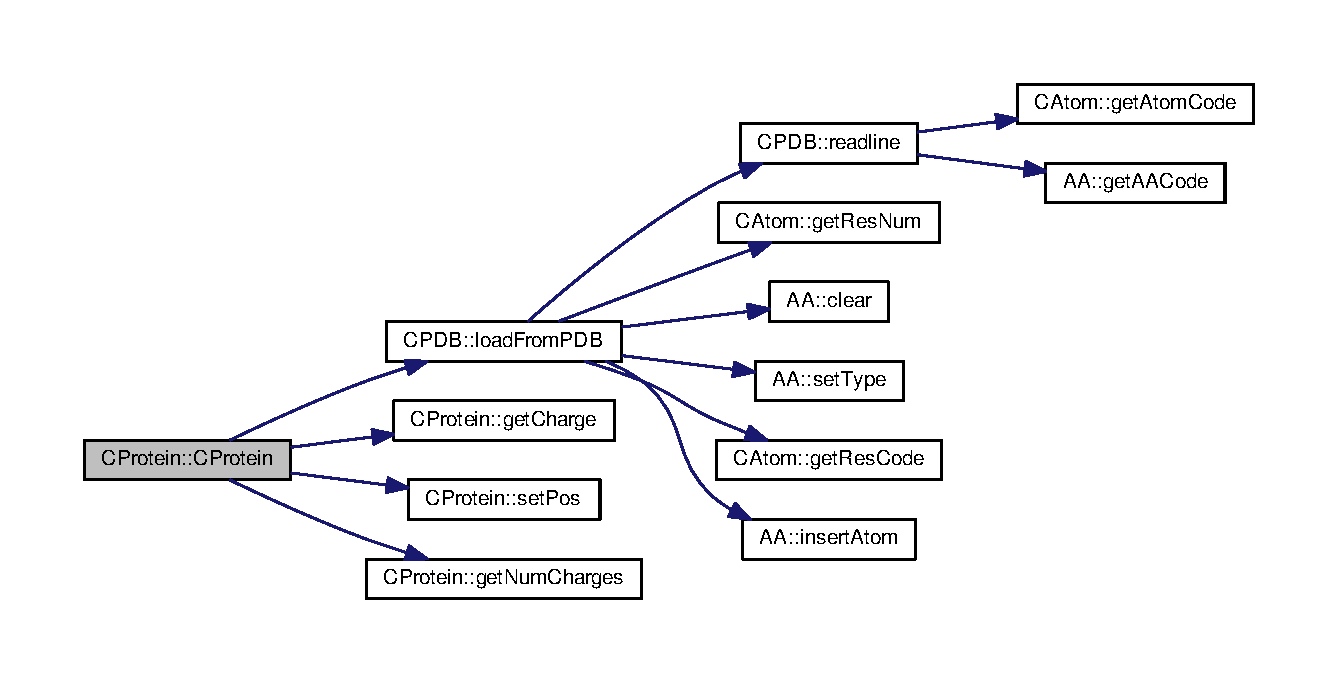
\includegraphics[width=350pt]{classCProtein_add7b99ce966900c95f6a0b5ce1d644ac_cgraph}
\end{center}
\end{figure}




\subsection{Member Function Documentation}
\hypertarget{classCProtein_a3d071c05412cb0f2a423920d5ae000dc}{\index{C\-Protein@{C\-Protein}!compute\-Distance@{compute\-Distance}}
\index{compute\-Distance@{compute\-Distance}!CProtein@{C\-Protein}}
\subsubsection[{compute\-Distance}]{\setlength{\rightskip}{0pt plus 5cm}static {\bf R\-E\-A\-L} C\-Protein\-::compute\-Distance (
\begin{DoxyParamCaption}
\item[{const {\bf C\-Protein} \&}]{p1, }
\item[{const {\bf C\-Protein} \&}]{p2}
\end{DoxyParamCaption}
)\hspace{0.3cm}{\ttfamily [inline]}, {\ttfamily [static]}}}\label{classCProtein_a3d071c05412cb0f2a423920d5ae000dc}


The protein compute\-Distance. 

\hyperlink{classCProtein}{C\-Protein} compute\-Distance function 
\begin{DoxyParams}{Parameters}
{\em p1} & a C\-G molecule object \\
\hline
{\em p2} & a second C\-G molecule object \\
\hline
\end{DoxyParams}
\begin{DoxyReturn}{Returns}
a floating point of the distance between the two objects 
\end{DoxyReturn}


Here is the call graph for this function\-:\nopagebreak
\begin{figure}[H]
\begin{center}
\leavevmode
\includegraphics[width=350pt]{classCProtein_a3d071c05412cb0f2a423920d5ae000dc_cgraph}
\end{center}
\end{figure}


\hypertarget{classCProtein_a7d6c3fb53c773ea006d123e35301d9b8}{\index{C\-Protein@{C\-Protein}!compute\-Forces@{compute\-Forces}}
\index{compute\-Forces@{compute\-Forces}!CProtein@{C\-Protein}}
\subsubsection[{compute\-Forces}]{\setlength{\rightskip}{0pt plus 5cm}void C\-Protein\-::compute\-Forces (
\begin{DoxyParamCaption}
\item[{vector$<$ {\bf C\-Pnt} $>$ \&}]{force, }
\item[{vector$<$ {\bf C\-Pnt} $>$ \&}]{torque}
\end{DoxyParamCaption}
)\hspace{0.3cm}{\ttfamily [static]}}}\label{classCProtein_a7d6c3fb53c773ea006d123e35301d9b8}


The protein compute\-Forces function. 

Function that computes forces and torques on a group of \hyperlink{classCProtein}{C\-Protein} objects 
\begin{DoxyParams}{Parameters}
{\em force} & a vector of forces \\
\hline
{\em torque} & a vector of torques\\
\hline
\end{DoxyParams}
Compute forces between molecules. Input\-: vector of forces and torques acting on each molecule in the system 

Here is the call graph for this function\-:
\nopagebreak
\begin{figure}[H]
\begin{center}
\leavevmode
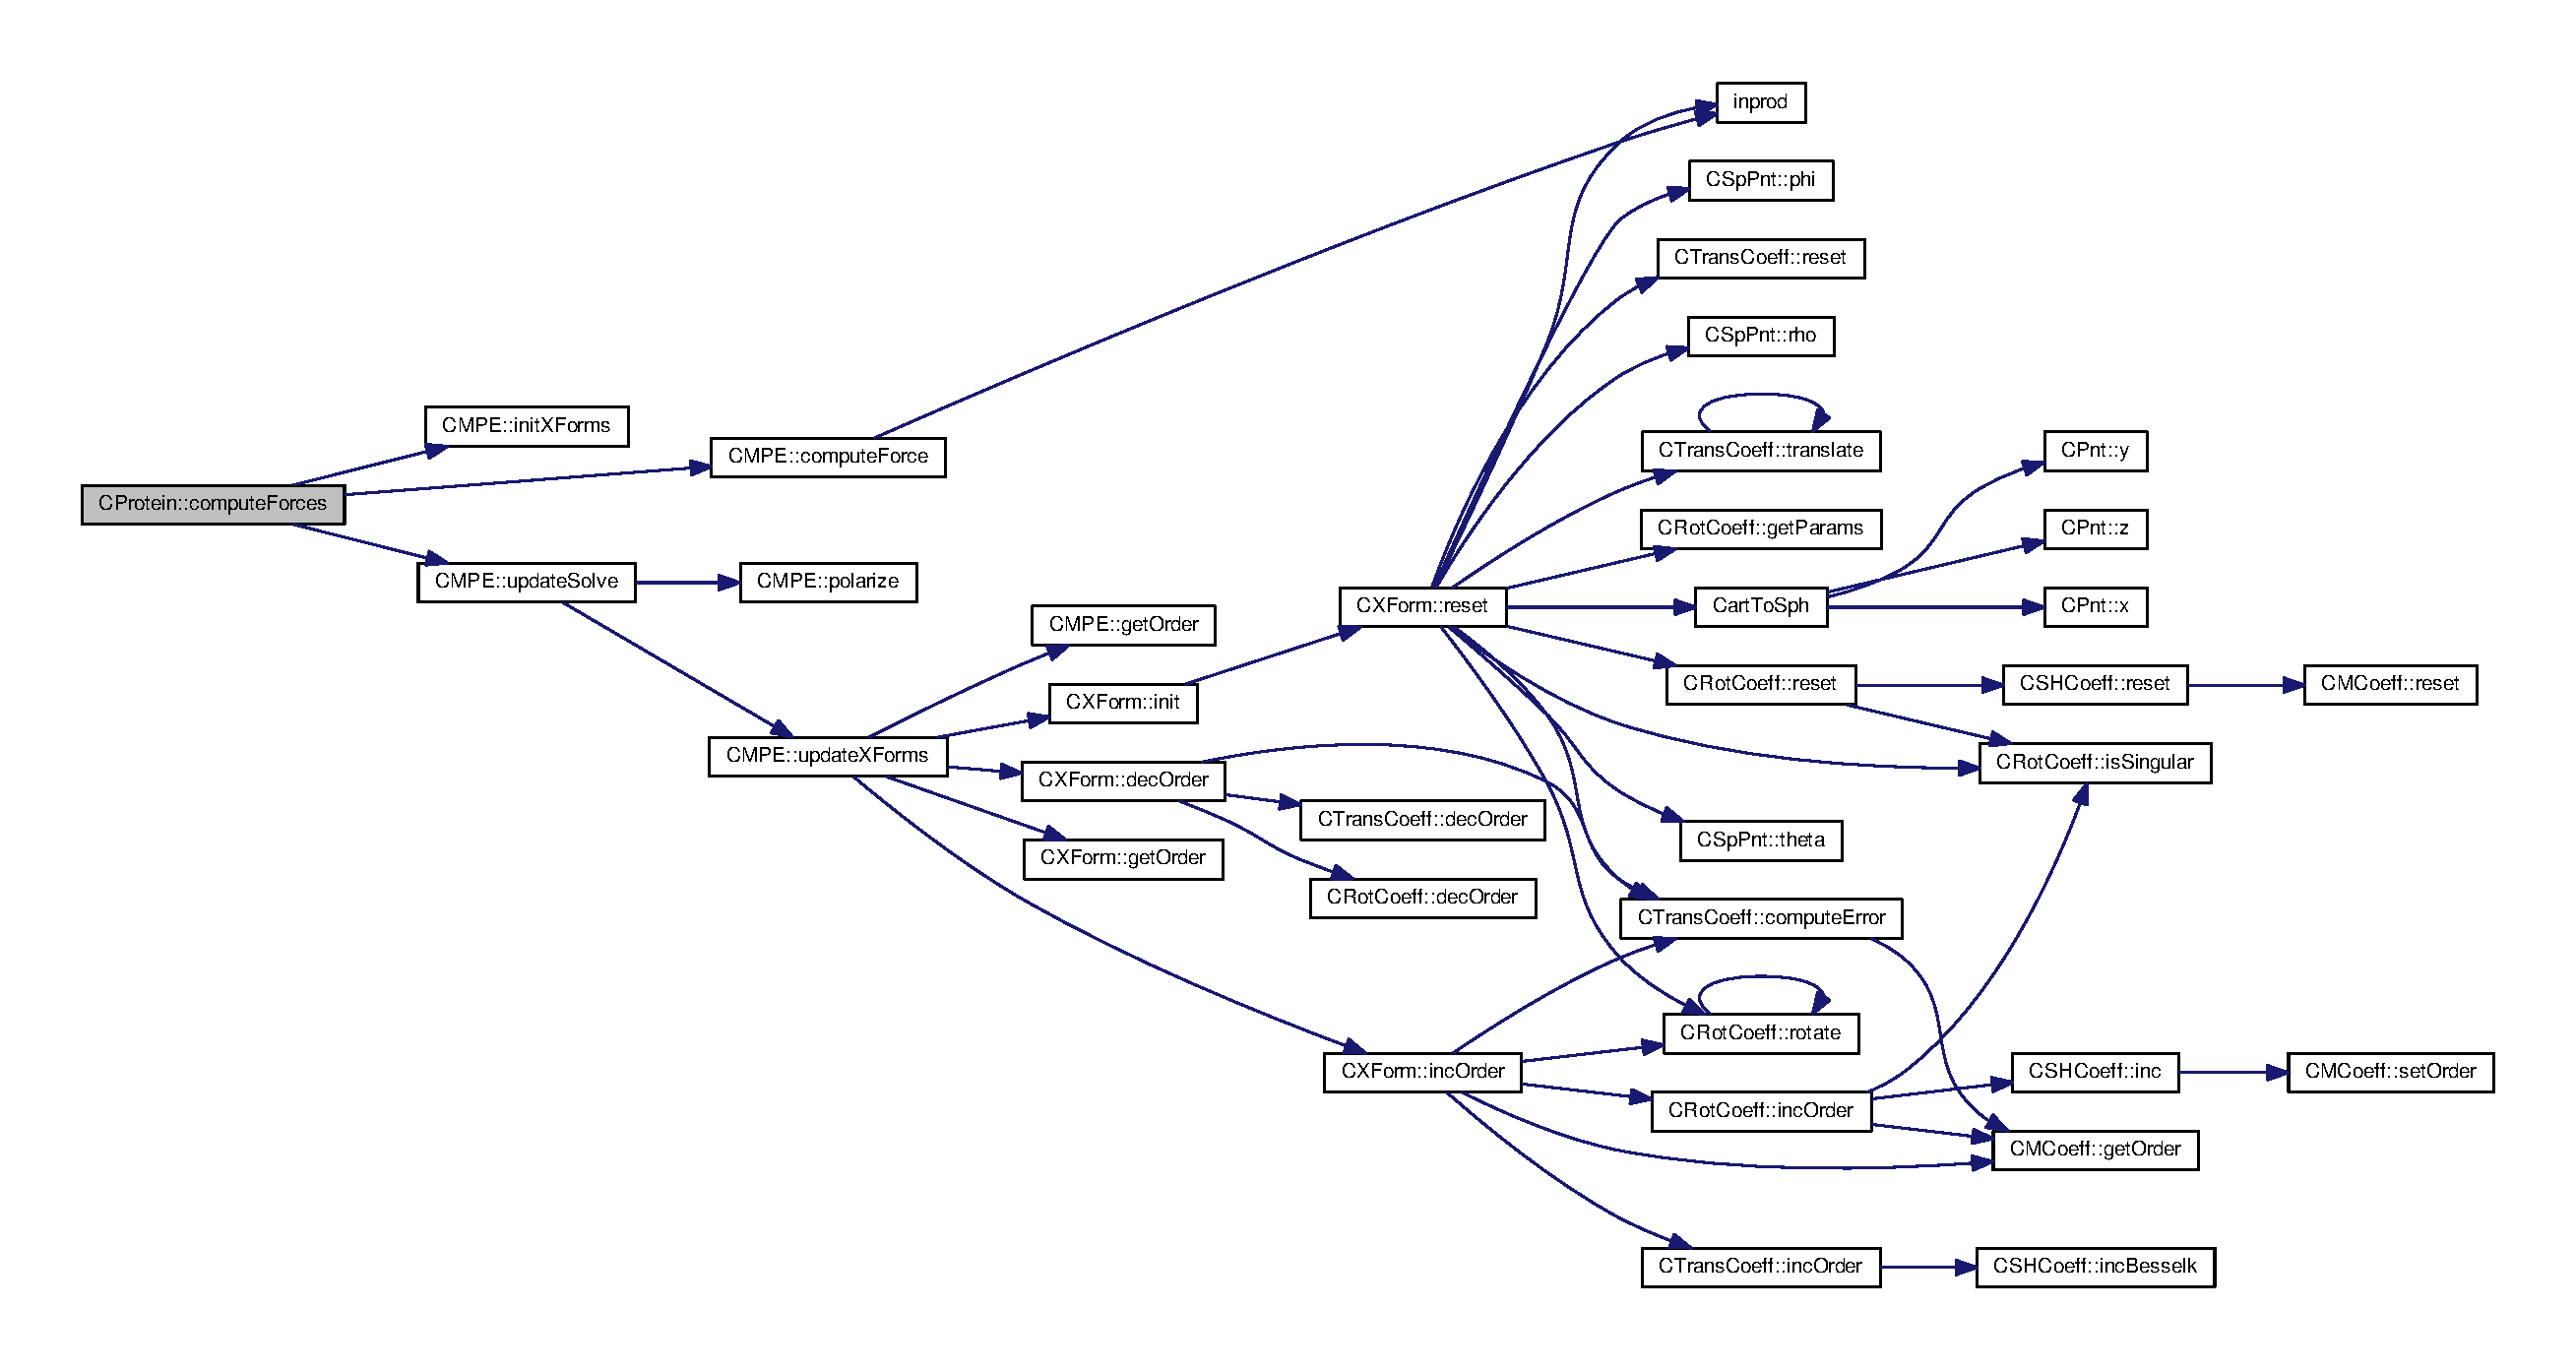
\includegraphics[width=350pt]{classCProtein_a7d6c3fb53c773ea006d123e35301d9b8_cgraph}
\end{center}
\end{figure}


\hypertarget{classCProtein_a61914554b1b927e7f2bfa4c12c78ba0a}{\index{C\-Protein@{C\-Protein}!get\-Atom@{get\-Atom}}
\index{get\-Atom@{get\-Atom}!CProtein@{C\-Protein}}
\subsubsection[{get\-Atom}]{\setlength{\rightskip}{0pt plus 5cm}const {\bf C\-Atom} $\ast$ C\-Protein\-::get\-Atom (
\begin{DoxyParamCaption}
\item[{int}]{resnum, }
\item[{int}]{acode}
\end{DoxyParamCaption}
) const}}\label{classCProtein_a61914554b1b927e7f2bfa4c12c78ba0a}


The protein get\-Atom function. 

Function that returns the desired atom 
\begin{DoxyParams}{Parameters}
{\em resnum} & an int of the residue number of the desired atom \\
\hline
{\em acode} & an int of the atom code of the desired atom\\
\hline
\end{DoxyParams}
Return atom of residue number resnum and atom code acode \hypertarget{classCProtein_ae44ab2afca86374611113fa26e8c1b2f}{\index{C\-Protein@{C\-Protein}!get\-Atoms@{get\-Atoms}}
\index{get\-Atoms@{get\-Atoms}!CProtein@{C\-Protein}}
\subsubsection[{get\-Atoms}]{\setlength{\rightskip}{0pt plus 5cm}const vector$<${\bf C\-Atom}$>$\& C\-Protein\-::get\-Atoms (
\begin{DoxyParamCaption}
{}
\end{DoxyParamCaption}
) const\hspace{0.3cm}{\ttfamily [inline]}}}\label{classCProtein_ae44ab2afca86374611113fa26e8c1b2f}
\hypertarget{classCProtein_a199bba5ba36900bdad8fd34bc0cc5342}{\index{C\-Protein@{C\-Protein}!get\-Charge@{get\-Charge}}
\index{get\-Charge@{get\-Charge}!CProtein@{C\-Protein}}
\subsubsection[{get\-Charge}]{\setlength{\rightskip}{0pt plus 5cm}{\bf R\-E\-A\-L} C\-Protein\-::get\-Charge (
\begin{DoxyParamCaption}
\item[{int}]{i}
\end{DoxyParamCaption}
) const\hspace{0.3cm}{\ttfamily [inline]}}}\label{classCProtein_a199bba5ba36900bdad8fd34bc0cc5342}


The protein get\-Charge. 

\hyperlink{classCProtein}{C\-Protein} get\-Charge function 
\begin{DoxyParams}{Parameters}
{\em i} & the ith atom in the protein for which to obtain charge \\
\hline
\end{DoxyParams}
\begin{DoxyReturn}{Returns}
a floating point of the charge at atom i 
\end{DoxyReturn}
\hypertarget{classCProtein_af41397ca141fb18b7a39854797e0df6a}{\index{C\-Protein@{C\-Protein}!get\-Charge\-Pos@{get\-Charge\-Pos}}
\index{get\-Charge\-Pos@{get\-Charge\-Pos}!CProtein@{C\-Protein}}
\subsubsection[{get\-Charge\-Pos}]{\setlength{\rightskip}{0pt plus 5cm}const {\bf C\-Pnt}\& C\-Protein\-::get\-Charge\-Pos (
\begin{DoxyParamCaption}
\item[{int}]{i}
\end{DoxyParamCaption}
) const\hspace{0.3cm}{\ttfamily [inline]}}}\label{classCProtein_af41397ca141fb18b7a39854797e0df6a}


The protein get\-Charge\-Pos. 

\hyperlink{classCProtein}{C\-Protein} get\-Charge\-Pos function 
\begin{DoxyParams}{Parameters}
{\em i} & the ith atom in the protein for which to obtain charge position \\
\hline
\end{DoxyParams}
\begin{DoxyReturn}{Returns}
a \hyperlink{classCPnt}{C\-Pnt} of the position of atom i 
\end{DoxyReturn}
\hypertarget{classCProtein_aa4cd0f117c25ed7e5a84db8e70147014}{\index{C\-Protein@{C\-Protein}!get\-I\-D@{get\-I\-D}}
\index{get\-I\-D@{get\-I\-D}!CProtein@{C\-Protein}}
\subsubsection[{get\-I\-D}]{\setlength{\rightskip}{0pt plus 5cm}int C\-Protein\-::get\-I\-D (
\begin{DoxyParamCaption}
{}
\end{DoxyParamCaption}
) const\hspace{0.3cm}{\ttfamily [inline]}}}\label{classCProtein_aa4cd0f117c25ed7e5a84db8e70147014}
\hypertarget{classCProtein_a2e38b7c42c30f967591fafb5060bc4f7}{\index{C\-Protein@{C\-Protein}!get\-Interface\-Atoms@{get\-Interface\-Atoms}}
\index{get\-Interface\-Atoms@{get\-Interface\-Atoms}!CProtein@{C\-Protein}}
\subsubsection[{get\-Interface\-Atoms}]{\setlength{\rightskip}{0pt plus 5cm}void C\-Protein\-::get\-Interface\-Atoms (
\begin{DoxyParamCaption}
\item[{const {\bf C\-Protein} \&}]{P1, }
\item[{const {\bf C\-Protein} \&}]{P2, }
\item[{vector$<$ {\bf C\-Pnt} $>$ \&}]{pos}
\end{DoxyParamCaption}
)\hspace{0.3cm}{\ttfamily [static]}}}\label{classCProtein_a2e38b7c42c30f967591fafb5060bc4f7}


The protein get\-Interface\-Atoms function. 

Function that returns a list of atoms at the interface 
\begin{DoxyParams}{Parameters}
{\em P1} & a \hyperlink{classCProtein}{C\-Protein} object \\
\hline
{\em P2} & a second \hyperlink{classCProtein}{C\-Protein} object that will dock with P1 \\
\hline
{\em pos} & a vector of positions of atoms at the P!-\/\-P2 interface\\
\hline
\end{DoxyParams}
Function that returns a list of atoms at the interface 

Here is the call graph for this function\-:\nopagebreak
\begin{figure}[H]
\begin{center}
\leavevmode
\includegraphics[width=350pt]{classCProtein_a2e38b7c42c30f967591fafb5060bc4f7_cgraph}
\end{center}
\end{figure}


\hypertarget{classCProtein_a8d680f9e8b07520eedfe5b43f50d1c03}{\index{C\-Protein@{C\-Protein}!get\-Num\-Charges@{get\-Num\-Charges}}
\index{get\-Num\-Charges@{get\-Num\-Charges}!CProtein@{C\-Protein}}
\subsubsection[{get\-Num\-Charges}]{\setlength{\rightskip}{0pt plus 5cm}int C\-Protein\-::get\-Num\-Charges (
\begin{DoxyParamCaption}
{}
\end{DoxyParamCaption}
) const\hspace{0.3cm}{\ttfamily [inline]}}}\label{classCProtein_a8d680f9e8b07520eedfe5b43f50d1c03}


The protein get\-Num\-Charges. 

\hyperlink{classCProtein}{C\-Protein} get\-Num\-Charges function \begin{DoxyReturn}{Returns}
the number of charges in the protein 
\end{DoxyReturn}
\hypertarget{classCProtein_a65cfe943745c04072d5a03b7caad861e}{\index{C\-Protein@{C\-Protein}!get\-Orientation@{get\-Orientation}}
\index{get\-Orientation@{get\-Orientation}!CProtein@{C\-Protein}}
\subsubsection[{get\-Orientation}]{\setlength{\rightskip}{0pt plus 5cm}const {\bf C\-Quat}\& C\-Protein\-::get\-Orientation (
\begin{DoxyParamCaption}
{}
\end{DoxyParamCaption}
) const\hspace{0.3cm}{\ttfamily [inline]}}}\label{classCProtein_a65cfe943745c04072d5a03b7caad861e}
\hypertarget{classCProtein_a1290a004e6e5854a8df7aa4acf9ba8e0}{\index{C\-Protein@{C\-Protein}!get\-Position@{get\-Position}}
\index{get\-Position@{get\-Position}!CProtein@{C\-Protein}}
\subsubsection[{get\-Position}]{\setlength{\rightskip}{0pt plus 5cm}const {\bf C\-Pnt}\& C\-Protein\-::get\-Position (
\begin{DoxyParamCaption}
{}
\end{DoxyParamCaption}
) const\hspace{0.3cm}{\ttfamily [inline]}}}\label{classCProtein_a1290a004e6e5854a8df7aa4acf9ba8e0}
\hypertarget{classCProtein_aaa51486082bb376c17cf272ed9ef6bca}{\index{C\-Protein@{C\-Protein}!get\-Radius@{get\-Radius}}
\index{get\-Radius@{get\-Radius}!CProtein@{C\-Protein}}
\subsubsection[{get\-Radius}]{\setlength{\rightskip}{0pt plus 5cm}{\bf R\-E\-A\-L} C\-Protein\-::get\-Radius (
\begin{DoxyParamCaption}
{}
\end{DoxyParamCaption}
) const\hspace{0.3cm}{\ttfamily [inline]}}}\label{classCProtein_aaa51486082bb376c17cf272ed9ef6bca}
\hypertarget{classCProtein_add93b850304f89cbb6af897e1df0fe4a}{\index{C\-Protein@{C\-Protein}!get\-Sum\-Charge@{get\-Sum\-Charge}}
\index{get\-Sum\-Charge@{get\-Sum\-Charge}!CProtein@{C\-Protein}}
\subsubsection[{get\-Sum\-Charge}]{\setlength{\rightskip}{0pt plus 5cm}{\bf R\-E\-A\-L} C\-Protein\-::get\-Sum\-Charge (
\begin{DoxyParamCaption}
{}
\end{DoxyParamCaption}
) const\hspace{0.3cm}{\ttfamily [inline]}}}\label{classCProtein_add93b850304f89cbb6af897e1df0fe4a}
\hypertarget{classCProtein_afb3fe3188e1a61488295b4fcdb3664e6}{\index{C\-Protein@{C\-Protein}!in\-Collision@{in\-Collision}}
\index{in\-Collision@{in\-Collision}!CProtein@{C\-Protein}}
\subsubsection[{in\-Collision}]{\setlength{\rightskip}{0pt plus 5cm}bool C\-Protein\-::in\-Collision (
\begin{DoxyParamCaption}
\item[{const {\bf C\-Protein} \&}]{mol}
\end{DoxyParamCaption}
)}}\label{classCProtein_afb3fe3188e1a61488295b4fcdb3664e6}


The protein in\-Collision function. 

Function that determines whether two molecules have collided or not 
\begin{DoxyParams}{Parameters}
{\em mol} & a vector of \hyperlink{classCProtein}{C\-Protein} objects \\
\hline
\end{DoxyParams}
\begin{DoxyReturn}{Returns}
a boolean indicating whether the molecules have collided (true)
\end{DoxyReturn}
Function to determine whether two C\-G molecules are collided or not 

Here is the call graph for this function\-:
\nopagebreak
\begin{figure}[H]
\begin{center}
\leavevmode
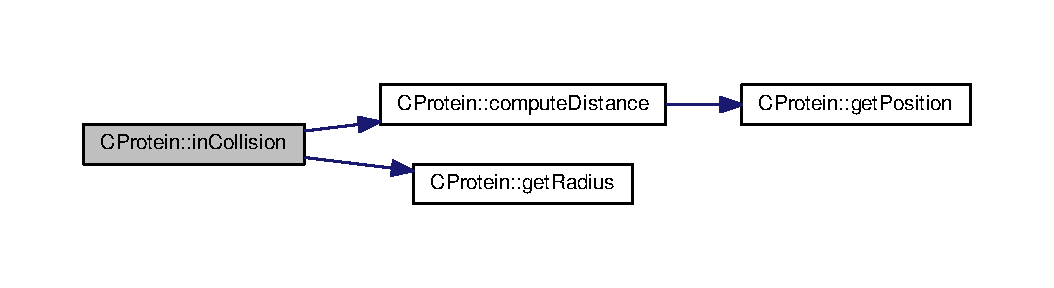
\includegraphics[width=350pt]{classCProtein_afb3fe3188e1a61488295b4fcdb3664e6_cgraph}
\end{center}
\end{figure}


\hypertarget{classCProtein_aeff60f05cbd42168359f75187b9ac888}{\index{C\-Protein@{C\-Protein}!init\-Parameters@{init\-Parameters}}
\index{init\-Parameters@{init\-Parameters}!CProtein@{C\-Protein}}
\subsubsection[{init\-Parameters}]{\setlength{\rightskip}{0pt plus 5cm}void C\-Protein\-::init\-Parameters (
\begin{DoxyParamCaption}
\item[{{\bf R\-E\-A\-L}}]{kappa, }
\item[{{\bf R\-E\-A\-L}}]{dielp, }
\item[{{\bf R\-E\-A\-L}}]{diels, }
\item[{int}]{nmol, }
\item[{{\bf R\-E\-A\-L}}]{rs}
\end{DoxyParamCaption}
)\hspace{0.3cm}{\ttfamily [static]}}}\label{classCProtein_aeff60f05cbd42168359f75187b9ac888}


The protein init\-Parameters function. 

Function that initializes parameters for a protein class 
\begin{DoxyParams}{Parameters}
{\em kappa} & the inverse debye length \\
\hline
{\em dielp} & the protein dielectric constant \\
\hline
{\em diels} & the solvent dielectric constant \\
\hline
{\em nmol} & the number of molecules in the system \\
\hline
{\em rs} & a scaling factor of the molecule\\
\hline
\end{DoxyParams}
Initializing parameters for protein file Inputs\-: kappa, dielectric of the protein, water dielectric, the nummber of molecules, average scaling factor R\-S$\sim$avg molecular radius 

Here is the call graph for this function\-:
\nopagebreak
\begin{figure}[H]
\begin{center}
\leavevmode
\includegraphics[width=350pt]{classCProtein_aeff60f05cbd42168359f75187b9ac888_cgraph}
\end{center}
\end{figure}


\hypertarget{classCProtein_a60767b1667e57c9a68045a6c148799cd}{\index{C\-Protein@{C\-Protein}!is\-Initialized@{is\-Initialized}}
\index{is\-Initialized@{is\-Initialized}!CProtein@{C\-Protein}}
\subsubsection[{is\-Initialized}]{\setlength{\rightskip}{0pt plus 5cm}static bool C\-Protein\-::is\-Initialized (
\begin{DoxyParamCaption}
{}
\end{DoxyParamCaption}
)\hspace{0.3cm}{\ttfamily [inline]}, {\ttfamily [static]}}}\label{classCProtein_a60767b1667e57c9a68045a6c148799cd}


The protein is\-Initialized. 

\hyperlink{classCProtein}{C\-Protein} is\-Initialized function, check if object's constants have been initialized \begin{DoxyReturn}{Returns}
a boolean of whether or not the system has been initialized 
\end{DoxyReturn}
\hypertarget{classCProtein_a2ab8b5e61cd26aafde2841b6b3655d45}{\index{C\-Protein@{C\-Protein}!rotate@{rotate}}
\index{rotate@{rotate}!CProtein@{C\-Protein}}
\subsubsection[{rotate}]{\setlength{\rightskip}{0pt plus 5cm}void C\-Protein\-::rotate (
\begin{DoxyParamCaption}
\item[{const {\bf C\-Quat} \&}]{rot}
\end{DoxyParamCaption}
)\hspace{0.3cm}{\ttfamily [inline]}}}\label{classCProtein_a2ab8b5e61cd26aafde2841b6b3655d45}


The protein rotate. 

\hyperlink{classCProtein}{C\-Protein} rotate function 
\begin{DoxyParams}{Parameters}
{\em rot} & a quaternion to rotate the \hyperlink{classCProtein}{C\-Protein} object by \\
\hline
\end{DoxyParams}
\hypertarget{classCProtein_a40f7c9e8d7b4717e00027b0c92ad109b}{\index{C\-Protein@{C\-Protein}!set\-Orient@{set\-Orient}}
\index{set\-Orient@{set\-Orient}!CProtein@{C\-Protein}}
\subsubsection[{set\-Orient}]{\setlength{\rightskip}{0pt plus 5cm}void C\-Protein\-::set\-Orient (
\begin{DoxyParamCaption}
\item[{const {\bf C\-Quat} \&}]{rot}
\end{DoxyParamCaption}
)\hspace{0.3cm}{\ttfamily [inline]}}}\label{classCProtein_a40f7c9e8d7b4717e00027b0c92ad109b}


The protein set\-Orient. 

\hyperlink{classCProtein}{C\-Protein} set\-Orient function 
\begin{DoxyParams}{Parameters}
{\em rot} & a quaterion to set the orientation of the molecule with \\
\hline
\end{DoxyParams}
\hypertarget{classCProtein_a890bc62459bae1a93b67e90cdcef18eb}{\index{C\-Protein@{C\-Protein}!set\-Pos@{set\-Pos}}
\index{set\-Pos@{set\-Pos}!CProtein@{C\-Protein}}
\subsubsection[{set\-Pos}]{\setlength{\rightskip}{0pt plus 5cm}void C\-Protein\-::set\-Pos (
\begin{DoxyParamCaption}
\item[{const {\bf C\-Pnt} \&}]{trans}
\end{DoxyParamCaption}
)\hspace{0.3cm}{\ttfamily [inline]}}}\label{classCProtein_a890bc62459bae1a93b67e90cdcef18eb}


The protein set\-Pos. 

\hyperlink{classCProtein}{C\-Protein} set\-Pos function 
\begin{DoxyParams}{Parameters}
{\em trans} & a vector of X\-Y\-Z coordinates to set the center at \\
\hline
\end{DoxyParams}
\hypertarget{classCProtein_a7d82de84256c6e9b5868b8fe08df6e15}{\index{C\-Protein@{C\-Protein}!translate@{translate}}
\index{translate@{translate}!CProtein@{C\-Protein}}
\subsubsection[{translate}]{\setlength{\rightskip}{0pt plus 5cm}void C\-Protein\-::translate (
\begin{DoxyParamCaption}
\item[{const {\bf C\-Pnt} \&}]{trans}
\end{DoxyParamCaption}
)\hspace{0.3cm}{\ttfamily [inline]}}}\label{classCProtein_a7d82de84256c6e9b5868b8fe08df6e15}


The protein translate. 

\hyperlink{classCProtein}{C\-Protein} translate function 
\begin{DoxyParams}{Parameters}
{\em trans} & a vector of X\-Y\-Z coordinates to translate the \hyperlink{classCProtein}{C\-Protein} object by \\
\hline
\end{DoxyParams}
\hypertarget{classCProtein_ac7497ee640c9910a3b05ed890845b118}{\index{C\-Protein@{C\-Protein}!untransform@{untransform}}
\index{untransform@{untransform}!CProtein@{C\-Protein}}
\subsubsection[{untransform}]{\setlength{\rightskip}{0pt plus 5cm}void C\-Protein\-::untransform (
\begin{DoxyParamCaption}
{}
\end{DoxyParamCaption}
)\hspace{0.3cm}{\ttfamily [inline]}}}\label{classCProtein_ac7497ee640c9910a3b05ed890845b118}


The protein untransform. 

\hyperlink{classCProtein}{C\-Protein} untransform function, move protein center back to saved location 

\subsection{Member Data Documentation}
\hypertarget{classCProtein_a5999d9758c6552f1c329cb3b5612485d}{\index{C\-Protein@{C\-Protein}!C\-H\-A\-R\-G\-E\-S@{C\-H\-A\-R\-G\-E\-S}}
\index{C\-H\-A\-R\-G\-E\-S@{C\-H\-A\-R\-G\-E\-S}!CProtein@{C\-Protein}}
\subsubsection[{C\-H\-A\-R\-G\-E\-S}]{\setlength{\rightskip}{0pt plus 5cm}map$<$ int, {\bf R\-E\-A\-L} $>$ C\-Protein\-::\-C\-H\-A\-R\-G\-E\-S\hspace{0.3cm}{\ttfamily [static]}}}\label{classCProtein_a5999d9758c6552f1c329cb3b5612485d}


Array of charges for each amino acid in the protein. 



The documentation for this class was generated from the following files\-:\begin{DoxyCompactItemize}
\item 
\hyperlink{protein_8h}{protein.\-h}\item 
\hyperlink{protein_8cpp}{protein.\-cpp}\end{DoxyCompactItemize}

\hypertarget{classCQuat}{\section{C\-Quat Class Reference}
\label{classCQuat}\index{C\-Quat@{C\-Quat}}
}


The quaternion class.  




{\ttfamily \#include $<$util.\-h$>$}

\subsection*{Public Member Functions}
\begin{DoxyCompactItemize}
\item 
\hyperlink{classCQuat_aa8497e624cd8c83814ee708beed80be8}{C\-Quat} ()
\begin{DoxyCompactList}\small\item\em The quaternion constructor. \end{DoxyCompactList}\item 
\hyperlink{classCQuat_a9e2eb21a9c7ec78d94e0fe38e34b242b}{C\-Quat} (\hyperlink{util_8h_a5821460e95a0800cf9f24c38915cbbde}{R\-E\-A\-L} \hyperlink{classCQuat_a7f18efa604d788a39bb6726de6546ce2}{real}, const \hyperlink{classCPnt}{C\-Pnt} \&\hyperlink{classCQuat_a783b34fbc307fbb00fd112c8441b0f30}{imag})
\begin{DoxyCompactList}\small\item\em The quaternion constructor. \end{DoxyCompactList}\item 
\hyperlink{classCQuat_a5225432b6d2298207cadd596073a500c}{C\-Quat} (const \hyperlink{classCPnt}{C\-Pnt} \&axis, \hyperlink{util_8h_a5821460e95a0800cf9f24c38915cbbde}{R\-E\-A\-L} angle)
\begin{DoxyCompactList}\small\item\em The quaternion constructor. \end{DoxyCompactList}\item 
\hyperlink{classCQuat_acd11b75e7090f6a6992425bcc5416219}{C\-Quat} (const \hyperlink{classCQuat}{C\-Quat} \&q)
\item 
\hyperlink{classCQuat}{C\-Quat} \& \hyperlink{classCQuat_ad7a24172721a059adcbf40f6db7584fb}{operator=} (const \hyperlink{classCQuat}{C\-Quat} \&q)
\item 
void \hyperlink{classCQuat_a9a0a307a7660ba46e1587b67f5cc35ea}{identity} ()
\begin{DoxyCompactList}\small\item\em \hyperlink{classCQuat}{C\-Quat} identity. \end{DoxyCompactList}\item 
\hyperlink{classCQuat}{C\-Quat} \& \hyperlink{classCQuat_a91a9f75dd706a025a68121522d30a561}{operator$\ast$=} (const \hyperlink{classCQuat}{C\-Quat} \&q)
\begin{DoxyCompactList}\small\item\em \hyperlink{classCQuat}{C\-Quat} $\ast$=. \end{DoxyCompactList}\item 
void \hyperlink{classCQuat_ab6e67daab741dfb157e3e5562a804706}{normalize} ()
\begin{DoxyCompactList}\small\item\em \hyperlink{classCQuat}{C\-Quat} normalize. \end{DoxyCompactList}\item 
void \hyperlink{classCQuat_a03c7815f439647be9e4cc8f3937cd0d0}{conj} ()
\begin{DoxyCompactList}\small\item\em \hyperlink{classCQuat}{C\-Quat} conj. \end{DoxyCompactList}\item 
\hyperlink{util_8h_a5821460e95a0800cf9f24c38915cbbde}{R\-E\-A\-L} \hyperlink{classCQuat_a7f18efa604d788a39bb6726de6546ce2}{real} () const 
\item 
const \hyperlink{classCPnt}{C\-Pnt} \& \hyperlink{classCQuat_a783b34fbc307fbb00fd112c8441b0f30}{imag} () const 
\item 
\hyperlink{util_8h_a5821460e95a0800cf9f24c38915cbbde}{R\-E\-A\-L} \hyperlink{classCQuat_ae6b5a06a27a9253ec3737101ddd02ee5}{x} () const 
\item 
\hyperlink{util_8h_a5821460e95a0800cf9f24c38915cbbde}{R\-E\-A\-L} \hyperlink{classCQuat_a01fcb600b793533c9f7554668739ac86}{y} () const 
\item 
\hyperlink{util_8h_a5821460e95a0800cf9f24c38915cbbde}{R\-E\-A\-L} \hyperlink{classCQuat_a1d2b9113413336187282a0dffcf5b39b}{z} () const 
\item 
\hyperlink{util_8h_a5821460e95a0800cf9f24c38915cbbde}{R\-E\-A\-L} \hyperlink{classCQuat_a8e83cf929e0e4f669482b419b20a096c}{w} () const 
\end{DoxyCompactItemize}
\subsection*{Static Public Member Functions}
\begin{DoxyCompactItemize}
\item 
static \hyperlink{classCQuat}{C\-Quat} \hyperlink{classCQuat_a3788f9ce393c8c6e7dc2df6e7675c594}{choose\-Random} ()
\begin{DoxyCompactList}\small\item\em \hyperlink{classCQuat}{C\-Quat} choose\-Random, choose random quaternion. \end{DoxyCompactList}\end{DoxyCompactItemize}
\subsection*{Friends}
\begin{DoxyCompactItemize}
\item 
\hyperlink{classCQuat}{C\-Quat} \hyperlink{classCQuat_a56293e53132060601a281240804d9302}{operator$\ast$} (const \hyperlink{classCQuat}{C\-Quat} \&q1, const \hyperlink{classCQuat}{C\-Quat} \&q2)
\begin{DoxyCompactList}\small\item\em \hyperlink{classCQuat}{C\-Quat} $\ast$. \end{DoxyCompactList}\item 
\hyperlink{classCPnt}{C\-Pnt} \hyperlink{classCQuat_ac98154ed89178004c9023423651b58a9}{operator$\ast$} (const \hyperlink{classCQuat}{C\-Quat} \&q1, const \hyperlink{classCPnt}{C\-Pnt} \&p1)
\begin{DoxyCompactList}\small\item\em \hyperlink{classCQuat}{C\-Quat} $\ast$ \hyperlink{classCPnt}{C\-Pnt}. \end{DoxyCompactList}\item 
\hyperlink{classCQuat}{C\-Quat} \hyperlink{classCQuat_a751f3ac0c157ff6967eaf2673ce1527e}{conj} (const \hyperlink{classCQuat}{C\-Quat} \&q)
\begin{DoxyCompactList}\small\item\em \hyperlink{classCQuat}{C\-Quat} conj. \end{DoxyCompactList}\item 
ostream \& \hyperlink{classCQuat_afeef42a3ba6ea600e39ee2accca10836}{operator$<$$<$} (ostream \&out, const \hyperlink{classCQuat}{C\-Quat} \&q)
\begin{DoxyCompactList}\small\item\em \hyperlink{classCQuat}{C\-Quat} $<$$<$. \end{DoxyCompactList}\end{DoxyCompactItemize}


\subsection{Detailed Description}
The quaternion class. 

The class that contains all details for a quaternion object. Quaterions can be used to describe spatial rotations in space. It is represented here as\-:

Q = m\-\_\-real + m\-\_\-imag.\-x$\ast$i + m\-\_\-imag.\-y$\ast$j + m\-\_\-imag.\-z$\ast$k

the conjugate is

Q.\-conj = m\-\_\-real -\/ m\-\_\-imag.\-x$\ast$i -\/ m\-\_\-imag.\-y$\ast$j -\/ m\-\_\-imag.\-z$\ast$k

For more, see \href{http://mathworld.wolfram.com/Quaternion.html}{\tt http\-://mathworld.\-wolfram.\-com/\-Quaternion.\-html} 

\subsection{Constructor \& Destructor Documentation}
\hypertarget{classCQuat_aa8497e624cd8c83814ee708beed80be8}{\index{C\-Quat@{C\-Quat}!C\-Quat@{C\-Quat}}
\index{C\-Quat@{C\-Quat}!CQuat@{C\-Quat}}
\subsubsection[{C\-Quat}]{\setlength{\rightskip}{0pt plus 5cm}C\-Quat\-::\-C\-Quat (
\begin{DoxyParamCaption}
{}
\end{DoxyParamCaption}
)\hspace{0.3cm}{\ttfamily [inline]}}}\label{classCQuat_aa8497e624cd8c83814ee708beed80be8}


The quaternion constructor. 

Create an identity quaternion object \hypertarget{classCQuat_a9e2eb21a9c7ec78d94e0fe38e34b242b}{\index{C\-Quat@{C\-Quat}!C\-Quat@{C\-Quat}}
\index{C\-Quat@{C\-Quat}!CQuat@{C\-Quat}}
\subsubsection[{C\-Quat}]{\setlength{\rightskip}{0pt plus 5cm}C\-Quat\-::\-C\-Quat (
\begin{DoxyParamCaption}
\item[{{\bf R\-E\-A\-L}}]{real, }
\item[{const {\bf C\-Pnt} \&}]{imag}
\end{DoxyParamCaption}
)\hspace{0.3cm}{\ttfamily [inline]}}}\label{classCQuat_a9e2eb21a9c7ec78d94e0fe38e34b242b}


The quaternion constructor. 

Create an identity quaternion object from real and imag components and normalize them. 
\begin{DoxyParams}{Parameters}
{\em real} & the real component of the quaternion \\
\hline
{\em imag} & a \hyperlink{classCPnt}{C\-Pnt} object of imaginary components for the quaternion \\
\hline
\end{DoxyParams}
\hypertarget{classCQuat_a5225432b6d2298207cadd596073a500c}{\index{C\-Quat@{C\-Quat}!C\-Quat@{C\-Quat}}
\index{C\-Quat@{C\-Quat}!CQuat@{C\-Quat}}
\subsubsection[{C\-Quat}]{\setlength{\rightskip}{0pt plus 5cm}C\-Quat\-::\-C\-Quat (
\begin{DoxyParamCaption}
\item[{const {\bf C\-Pnt} \&}]{axis, }
\item[{{\bf R\-E\-A\-L}}]{angle}
\end{DoxyParamCaption}
)\hspace{0.3cm}{\ttfamily [inline]}}}\label{classCQuat_a5225432b6d2298207cadd596073a500c}


The quaternion constructor. 

Create an identity quaternion object from an axis and an angle 
\begin{DoxyParams}{Parameters}
{\em axis} & a vector defining an axis of rotation \\
\hline
{\em angle} & an angle to rotate around the axis by in radians \\
\hline
\end{DoxyParams}
\hypertarget{classCQuat_acd11b75e7090f6a6992425bcc5416219}{\index{C\-Quat@{C\-Quat}!C\-Quat@{C\-Quat}}
\index{C\-Quat@{C\-Quat}!CQuat@{C\-Quat}}
\subsubsection[{C\-Quat}]{\setlength{\rightskip}{0pt plus 5cm}C\-Quat\-::\-C\-Quat (
\begin{DoxyParamCaption}
\item[{const {\bf C\-Quat} \&}]{q}
\end{DoxyParamCaption}
)\hspace{0.3cm}{\ttfamily [inline]}}}\label{classCQuat_acd11b75e7090f6a6992425bcc5416219}


\subsection{Member Function Documentation}
\hypertarget{classCQuat_a3788f9ce393c8c6e7dc2df6e7675c594}{\index{C\-Quat@{C\-Quat}!choose\-Random@{choose\-Random}}
\index{choose\-Random@{choose\-Random}!CQuat@{C\-Quat}}
\subsubsection[{choose\-Random}]{\setlength{\rightskip}{0pt plus 5cm}{\bf C\-Quat} C\-Quat\-::choose\-Random (
\begin{DoxyParamCaption}
{}
\end{DoxyParamCaption}
)\hspace{0.3cm}{\ttfamily [inline]}, {\ttfamily [static]}}}\label{classCQuat_a3788f9ce393c8c6e7dc2df6e7675c594}


\hyperlink{classCQuat}{C\-Quat} choose\-Random, choose random quaternion. 

\hyperlink{classCQuat}{C\-Quat} choose\-Random.

Choose a random quaternion \hypertarget{classCQuat_a03c7815f439647be9e4cc8f3937cd0d0}{\index{C\-Quat@{C\-Quat}!conj@{conj}}
\index{conj@{conj}!CQuat@{C\-Quat}}
\subsubsection[{conj}]{\setlength{\rightskip}{0pt plus 5cm}void C\-Quat\-::conj (
\begin{DoxyParamCaption}
{}
\end{DoxyParamCaption}
)\hspace{0.3cm}{\ttfamily [inline]}}}\label{classCQuat_a03c7815f439647be9e4cc8f3937cd0d0}


\hyperlink{classCQuat}{C\-Quat} conj. 

Set the imaginary part to their conjugates. \hypertarget{classCQuat_a9a0a307a7660ba46e1587b67f5cc35ea}{\index{C\-Quat@{C\-Quat}!identity@{identity}}
\index{identity@{identity}!CQuat@{C\-Quat}}
\subsubsection[{identity}]{\setlength{\rightskip}{0pt plus 5cm}void C\-Quat\-::identity (
\begin{DoxyParamCaption}
{}
\end{DoxyParamCaption}
)\hspace{0.3cm}{\ttfamily [inline]}}}\label{classCQuat_a9a0a307a7660ba46e1587b67f5cc35ea}


\hyperlink{classCQuat}{C\-Quat} identity. 

Generate the identity quaternion, with imag parts set to (0,0,0) and the real part to 1.\-0 \hypertarget{classCQuat_a783b34fbc307fbb00fd112c8441b0f30}{\index{C\-Quat@{C\-Quat}!imag@{imag}}
\index{imag@{imag}!CQuat@{C\-Quat}}
\subsubsection[{imag}]{\setlength{\rightskip}{0pt plus 5cm}const {\bf C\-Pnt}\& C\-Quat\-::imag (
\begin{DoxyParamCaption}
{}
\end{DoxyParamCaption}
) const\hspace{0.3cm}{\ttfamily [inline]}}}\label{classCQuat_a783b34fbc307fbb00fd112c8441b0f30}
\hypertarget{classCQuat_ab6e67daab741dfb157e3e5562a804706}{\index{C\-Quat@{C\-Quat}!normalize@{normalize}}
\index{normalize@{normalize}!CQuat@{C\-Quat}}
\subsubsection[{normalize}]{\setlength{\rightskip}{0pt plus 5cm}void C\-Quat\-::normalize (
\begin{DoxyParamCaption}
{}
\end{DoxyParamCaption}
)\hspace{0.3cm}{\ttfamily [inline]}}}\label{classCQuat_ab6e67daab741dfb157e3e5562a804706}


\hyperlink{classCQuat}{C\-Quat} normalize. 

Normalize the quaternion, compute the norm and then reset the imaginary and real parts of the quaternion \hypertarget{classCQuat_a91a9f75dd706a025a68121522d30a561}{\index{C\-Quat@{C\-Quat}!operator$\ast$=@{operator$\ast$=}}
\index{operator$\ast$=@{operator$\ast$=}!CQuat@{C\-Quat}}
\subsubsection[{operator$\ast$=}]{\setlength{\rightskip}{0pt plus 5cm}{\bf C\-Quat} \& C\-Quat\-::operator$\ast$= (
\begin{DoxyParamCaption}
\item[{const {\bf C\-Quat} \&}]{q}
\end{DoxyParamCaption}
)\hspace{0.3cm}{\ttfamily [inline]}}}\label{classCQuat_a91a9f75dd706a025a68121522d30a561}


\hyperlink{classCQuat}{C\-Quat} $\ast$=. 

Multiplying one quaternion by another 

Here is the call graph for this function\-:
\nopagebreak
\begin{figure}[H]
\begin{center}
\leavevmode
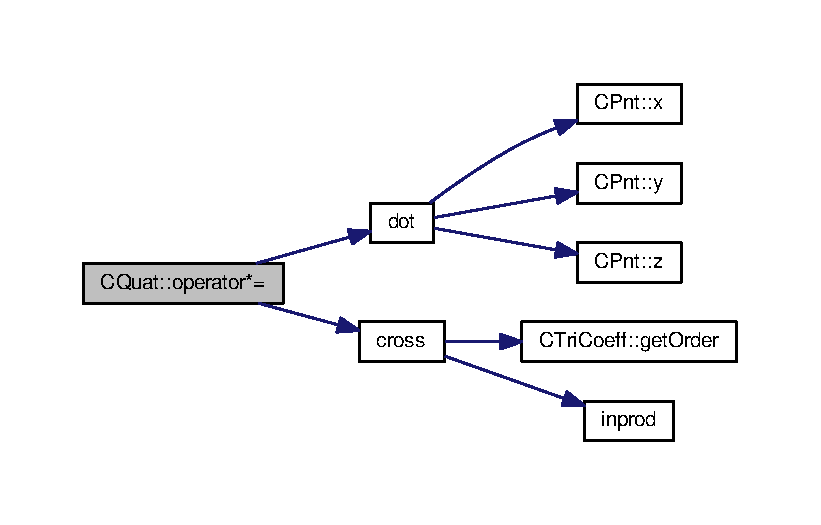
\includegraphics[width=350pt]{classCQuat_a91a9f75dd706a025a68121522d30a561_cgraph}
\end{center}
\end{figure}


\hypertarget{classCQuat_ad7a24172721a059adcbf40f6db7584fb}{\index{C\-Quat@{C\-Quat}!operator=@{operator=}}
\index{operator=@{operator=}!CQuat@{C\-Quat}}
\subsubsection[{operator=}]{\setlength{\rightskip}{0pt plus 5cm}{\bf C\-Quat}\& C\-Quat\-::operator= (
\begin{DoxyParamCaption}
\item[{const {\bf C\-Quat} \&}]{q}
\end{DoxyParamCaption}
)\hspace{0.3cm}{\ttfamily [inline]}}}\label{classCQuat_ad7a24172721a059adcbf40f6db7584fb}
\hypertarget{classCQuat_a7f18efa604d788a39bb6726de6546ce2}{\index{C\-Quat@{C\-Quat}!real@{real}}
\index{real@{real}!CQuat@{C\-Quat}}
\subsubsection[{real}]{\setlength{\rightskip}{0pt plus 5cm}{\bf R\-E\-A\-L} C\-Quat\-::real (
\begin{DoxyParamCaption}
{}
\end{DoxyParamCaption}
) const\hspace{0.3cm}{\ttfamily [inline]}}}\label{classCQuat_a7f18efa604d788a39bb6726de6546ce2}
\hypertarget{classCQuat_a8e83cf929e0e4f669482b419b20a096c}{\index{C\-Quat@{C\-Quat}!w@{w}}
\index{w@{w}!CQuat@{C\-Quat}}
\subsubsection[{w}]{\setlength{\rightskip}{0pt plus 5cm}{\bf R\-E\-A\-L} C\-Quat\-::w (
\begin{DoxyParamCaption}
{}
\end{DoxyParamCaption}
) const\hspace{0.3cm}{\ttfamily [inline]}}}\label{classCQuat_a8e83cf929e0e4f669482b419b20a096c}
\hypertarget{classCQuat_ae6b5a06a27a9253ec3737101ddd02ee5}{\index{C\-Quat@{C\-Quat}!x@{x}}
\index{x@{x}!CQuat@{C\-Quat}}
\subsubsection[{x}]{\setlength{\rightskip}{0pt plus 5cm}{\bf R\-E\-A\-L} C\-Quat\-::x (
\begin{DoxyParamCaption}
{}
\end{DoxyParamCaption}
) const\hspace{0.3cm}{\ttfamily [inline]}}}\label{classCQuat_ae6b5a06a27a9253ec3737101ddd02ee5}


Here is the call graph for this function\-:\nopagebreak
\begin{figure}[H]
\begin{center}
\leavevmode
\includegraphics[width=222pt]{classCQuat_ae6b5a06a27a9253ec3737101ddd02ee5_cgraph}
\end{center}
\end{figure}


\hypertarget{classCQuat_a01fcb600b793533c9f7554668739ac86}{\index{C\-Quat@{C\-Quat}!y@{y}}
\index{y@{y}!CQuat@{C\-Quat}}
\subsubsection[{y}]{\setlength{\rightskip}{0pt plus 5cm}{\bf R\-E\-A\-L} C\-Quat\-::y (
\begin{DoxyParamCaption}
{}
\end{DoxyParamCaption}
) const\hspace{0.3cm}{\ttfamily [inline]}}}\label{classCQuat_a01fcb600b793533c9f7554668739ac86}
\hypertarget{classCQuat_a1d2b9113413336187282a0dffcf5b39b}{\index{C\-Quat@{C\-Quat}!z@{z}}
\index{z@{z}!CQuat@{C\-Quat}}
\subsubsection[{z}]{\setlength{\rightskip}{0pt plus 5cm}{\bf R\-E\-A\-L} C\-Quat\-::z (
\begin{DoxyParamCaption}
{}
\end{DoxyParamCaption}
) const\hspace{0.3cm}{\ttfamily [inline]}}}\label{classCQuat_a1d2b9113413336187282a0dffcf5b39b}


\subsection{Friends And Related Function Documentation}
\hypertarget{classCQuat_a751f3ac0c157ff6967eaf2673ce1527e}{\index{C\-Quat@{C\-Quat}!conj@{conj}}
\index{conj@{conj}!CQuat@{C\-Quat}}
\subsubsection[{conj}]{\setlength{\rightskip}{0pt plus 5cm}{\bf C\-Quat} conj (
\begin{DoxyParamCaption}
\item[{const {\bf C\-Quat} \&}]{q}
\end{DoxyParamCaption}
)\hspace{0.3cm}{\ttfamily [friend]}}}\label{classCQuat_a751f3ac0c157ff6967eaf2673ce1527e}


\hyperlink{classCQuat}{C\-Quat} conj. 

Return complex conjugate of a quaternion \hypertarget{classCQuat_a56293e53132060601a281240804d9302}{\index{C\-Quat@{C\-Quat}!operator$\ast$@{operator$\ast$}}
\index{operator$\ast$@{operator$\ast$}!CQuat@{C\-Quat}}
\subsubsection[{operator$\ast$}]{\setlength{\rightskip}{0pt plus 5cm}{\bf C\-Quat} operator$\ast$ (
\begin{DoxyParamCaption}
\item[{const {\bf C\-Quat} \&}]{q1, }
\item[{const {\bf C\-Quat} \&}]{q2}
\end{DoxyParamCaption}
)\hspace{0.3cm}{\ttfamily [friend]}}}\label{classCQuat_a56293e53132060601a281240804d9302}


\hyperlink{classCQuat}{C\-Quat} $\ast$. 

Multiplying one quaternion by another \hypertarget{classCQuat_ac98154ed89178004c9023423651b58a9}{\index{C\-Quat@{C\-Quat}!operator$\ast$@{operator$\ast$}}
\index{operator$\ast$@{operator$\ast$}!CQuat@{C\-Quat}}
\subsubsection[{operator$\ast$}]{\setlength{\rightskip}{0pt plus 5cm}{\bf C\-Pnt} operator$\ast$ (
\begin{DoxyParamCaption}
\item[{const {\bf C\-Quat} \&}]{q1, }
\item[{const {\bf C\-Pnt} \&}]{p1}
\end{DoxyParamCaption}
)\hspace{0.3cm}{\ttfamily [friend]}}}\label{classCQuat_ac98154ed89178004c9023423651b58a9}


\hyperlink{classCQuat}{C\-Quat} $\ast$ \hyperlink{classCPnt}{C\-Pnt}. 

Multiplying quaternion by cartesian coordinates, for rotation \hypertarget{classCQuat_afeef42a3ba6ea600e39ee2accca10836}{\index{C\-Quat@{C\-Quat}!operator$<$$<$@{operator$<$$<$}}
\index{operator$<$$<$@{operator$<$$<$}!CQuat@{C\-Quat}}
\subsubsection[{operator$<$$<$}]{\setlength{\rightskip}{0pt plus 5cm}ostream\& operator$<$$<$ (
\begin{DoxyParamCaption}
\item[{ostream \&}]{out, }
\item[{const {\bf C\-Quat} \&}]{q}
\end{DoxyParamCaption}
)\hspace{0.3cm}{\ttfamily [friend]}}}\label{classCQuat_afeef42a3ba6ea600e39ee2accca10836}


\hyperlink{classCQuat}{C\-Quat} $<$$<$. 

Print out quaternion 

The documentation for this class was generated from the following file\-:\begin{DoxyCompactItemize}
\item 
\hyperlink{util_8h}{util.\-h}\end{DoxyCompactItemize}

\hypertarget{classCRotCoeff}{\section{C\-Rot\-Coeff Class Reference}
\label{classCRotCoeff}\index{C\-Rot\-Coeff@{C\-Rot\-Coeff}}
}


The rotation coefficient class.  




{\ttfamily \#include $<$rotcoeff.\-h$>$}

\subsection*{Public Member Functions}
\begin{DoxyCompactItemize}
\item 
\hyperlink{classCRotCoeff_a5dae485fb061a3c231365159aefc9bb5}{C\-Rot\-Coeff} (bool b\-Grad=true)
\begin{DoxyCompactList}\small\item\em The rotation coefficient class constructor. \end{DoxyCompactList}\item 
void \hyperlink{classCRotCoeff_aa52111e9c4cb2949dfae960437742536}{reset} (\hyperlink{util_8h_a5821460e95a0800cf9f24c38915cbbde}{R\-E\-A\-L} theta, \hyperlink{util_8h_a5821460e95a0800cf9f24c38915cbbde}{R\-E\-A\-L} phi, \hyperlink{util_8h_a5821460e95a0800cf9f24c38915cbbde}{R\-E\-A\-L} xi, int p)
\item 
void \hyperlink{classCRotCoeff_a4a6461f2947e6c07d4a28da4d87a8935}{reset} (const \hyperlink{classCPnt}{C\-Pnt} \&axis, \hyperlink{util_8h_a5821460e95a0800cf9f24c38915cbbde}{R\-E\-A\-L} ang, int p)
\item 
void \hyperlink{classCRotCoeff_a6dea4a3900cc4ac8c012cc8790b92719}{reset} (const \hyperlink{classCQuat}{C\-Quat} \&Q, int p)
\item 
void \hyperlink{classCRotCoeff_aa9b14ebaa2c45a8fa740fa36d9f31d2c}{rotate} (const \hyperlink{classCTriCoeff}{C\-Tri\-Coeff} \&Tin, \hyperlink{classCTriCoeff}{C\-Tri\-Coeff} \&Tout, bool b\-For)
\begin{DoxyCompactList}\small\item\em \hyperlink{classCRotCoeff}{C\-Rot\-Coeff} rotate function. \end{DoxyCompactList}\item 
void \hyperlink{classCRotCoeff_a6d65091921f8baa2175c97758dff4e16}{rotate} (const \hyperlink{classCTriCoeff}{C\-Tri\-Coeff} \&Tin, \hyperlink{classCTriCoeff}{C\-Tri\-Coeff} \&Tout, int p1, int p2, bool b\-For)
\begin{DoxyCompactList}\small\item\em \hyperlink{classCRotCoeff}{C\-Rot\-Coeff} rotate function. \end{DoxyCompactList}\item 
void \hyperlink{classCRotCoeff_a319c60548de84e430bd55f17d020fa3f}{rotate} (const \hyperlink{classCMCoeff}{C\-M\-Coeff} \&Min, \hyperlink{classCMCoeff}{C\-M\-Coeff} \&Mout, bool b\-For)
\begin{DoxyCompactList}\small\item\em \hyperlink{classCRotCoeff}{C\-Rot\-Coeff} rotate function. \end{DoxyCompactList}\item 
void \hyperlink{classCRotCoeff_ab93dd694803d34505c026b6d48bb6d25}{rotate} (const \hyperlink{classCMCoeff}{C\-M\-Coeff} \&Min, \hyperlink{classCMCoeff}{C\-M\-Coeff} \&Mout, int p1, int p2, bool b\-For)
\begin{DoxyCompactList}\small\item\em \hyperlink{classCRotCoeff}{C\-Rot\-Coeff} rotate function. \end{DoxyCompactList}\item 
void \hyperlink{classCRotCoeff_a73c21837871db96b643b0e9ccf77a6b4}{d\-Rotate\-T} (const \hyperlink{classCMCoeff}{C\-M\-Coeff} \&Min, \hyperlink{classCMCoeff}{C\-M\-Coeff} \&Mout, bool b\-For)
\begin{DoxyCompactList}\small\item\em \hyperlink{classCRotCoeff}{C\-Rot\-Coeff} d\-Rotate\-T function. \end{DoxyCompactList}\item 
void \hyperlink{classCRotCoeff_ab40b0a7225f78c026e488950545a33d6}{d\-Rotate\-T} (const \hyperlink{classCMCoeff}{C\-M\-Coeff} \&Min, \hyperlink{classCMCoeff}{C\-M\-Coeff} \&Mout, int p1, int p2, bool b\-For)
\begin{DoxyCompactList}\small\item\em \hyperlink{classCRotCoeff}{C\-Rot\-Coeff} d\-Rotate\-T function. \end{DoxyCompactList}\item 
void \hyperlink{classCRotCoeff_a8fc43b5ba7290e8f59fe124105445542}{d\-Rotate\-P} (const \hyperlink{classCMCoeff}{C\-M\-Coeff} \&Min, \hyperlink{classCMCoeff}{C\-M\-Coeff} \&Mout, bool b\-For)
\begin{DoxyCompactList}\small\item\em \hyperlink{classCRotCoeff}{C\-Rot\-Coeff} d\-Rotate\-P function. \end{DoxyCompactList}\item 
void \hyperlink{classCRotCoeff_a88d3ed40239b588e18399c549509f687}{d\-Rotate\-P} (const \hyperlink{classCMCoeff}{C\-M\-Coeff} \&Min, \hyperlink{classCMCoeff}{C\-M\-Coeff} \&Mout, int p1, int p2, bool b\-For)
\begin{DoxyCompactList}\small\item\em \hyperlink{classCRotCoeff}{C\-Rot\-Coeff} d\-Rotate\-P function. \end{DoxyCompactList}\item 
void \hyperlink{classCRotCoeff_a1416603a77ab7c9b7af515a7bad684f1}{inc\-Order} ()
\item 
void \hyperlink{classCRotCoeff_ae9fa83e941510deeda3aac1b8aecc58b}{dec\-Order} ()
\item 
void \hyperlink{classCRotCoeff_a505db8551887fabe49b0f7b6076c2060}{output\-Rot} (int p) const 
\item 
void \hyperlink{classCRotCoeff_a23dff497ccb1ca53dba01af9a27fdab8}{outputd\-Rot} (int p) const 
\item 
void \hyperlink{classCRotCoeff_acf2c3650570013fee7e54491fa1d5920}{save\-Undo} ()
\begin{DoxyCompactList}\small\item\em \hyperlink{classCRotCoeff}{C\-Rot\-Coeff} save\-Undo. \end{DoxyCompactList}\item 
void \hyperlink{classCRotCoeff_a976ea6ff504912701f549e988fd217dc}{undo} ()
\begin{DoxyCompactList}\small\item\em \hyperlink{classCRotCoeff}{C\-Rot\-Coeff} undo. \end{DoxyCompactList}\item 
bool \hyperlink{classCRotCoeff_a4668070c3eacacf17be98bc2fb348287}{is\-Singular} () const 
\item 
void \hyperlink{classCRotCoeff_a27b0198e460737ea20601fa4f0667df5}{get\-Params} (\hyperlink{util_8h_a5821460e95a0800cf9f24c38915cbbde}{R\-E\-A\-L} \&st, \hyperlink{util_8h_a5821460e95a0800cf9f24c38915cbbde}{R\-E\-A\-L} \&ct, \hyperlink{util_8h_a5821460e95a0800cf9f24c38915cbbde}{R\-E\-A\-L} \&sp, \hyperlink{util_8h_a5821460e95a0800cf9f24c38915cbbde}{R\-E\-A\-L} \&cp) const 
\end{DoxyCompactItemize}
\subsection*{Static Public Member Functions}
\begin{DoxyCompactItemize}
\item 
static void \hyperlink{classCRotCoeff_aa51371c84f373916cd8e35031b38cb52}{init\-Constants} ()
\begin{DoxyCompactList}\small\item\em The rotation coefficient init\-Constants function. \end{DoxyCompactList}\end{DoxyCompactItemize}


\subsection{Detailed Description}
The rotation coefficient class. 

The class that contains all details for rotation coefficients, which are described in the Appendix, section A.\-1 of Lotan 2006. 

\subsection{Constructor \& Destructor Documentation}
\hypertarget{classCRotCoeff_a5dae485fb061a3c231365159aefc9bb5}{\index{C\-Rot\-Coeff@{C\-Rot\-Coeff}!C\-Rot\-Coeff@{C\-Rot\-Coeff}}
\index{C\-Rot\-Coeff@{C\-Rot\-Coeff}!CRotCoeff@{C\-Rot\-Coeff}}
\subsubsection[{C\-Rot\-Coeff}]{\setlength{\rightskip}{0pt plus 5cm}C\-Rot\-Coeff\-::\-C\-Rot\-Coeff (
\begin{DoxyParamCaption}
\item[{bool}]{b\-Grad = {\ttfamily true}}
\end{DoxyParamCaption}
)}}\label{classCRotCoeff_a5dae485fb061a3c231365159aefc9bb5}


The rotation coefficient class constructor. 

This creates an object of the Rot\-Coeff class, using input of the user. Sets b\-Sing to false and N\-P\-O\-L\-E\-S to 1 
\begin{DoxyParams}{Parameters}
{\em b\-Grad} & a boolean that identifies whether or not the gradients of rotation coefficients should be computed or not. Default is yes.\\
\hline
\end{DoxyParams}
The rotation coefficient class constructor 

\subsection{Member Function Documentation}
\hypertarget{classCRotCoeff_ae9fa83e941510deeda3aac1b8aecc58b}{\index{C\-Rot\-Coeff@{C\-Rot\-Coeff}!dec\-Order@{dec\-Order}}
\index{dec\-Order@{dec\-Order}!CRotCoeff@{C\-Rot\-Coeff}}
\subsubsection[{dec\-Order}]{\setlength{\rightskip}{0pt plus 5cm}void C\-Rot\-Coeff\-::dec\-Order (
\begin{DoxyParamCaption}
{}
\end{DoxyParamCaption}
)\hspace{0.3cm}{\ttfamily [inline]}}}\label{classCRotCoeff_ae9fa83e941510deeda3aac1b8aecc58b}
\hypertarget{classCRotCoeff_a8fc43b5ba7290e8f59fe124105445542}{\index{C\-Rot\-Coeff@{C\-Rot\-Coeff}!d\-Rotate\-P@{d\-Rotate\-P}}
\index{d\-Rotate\-P@{d\-Rotate\-P}!CRotCoeff@{C\-Rot\-Coeff}}
\subsubsection[{d\-Rotate\-P}]{\setlength{\rightskip}{0pt plus 5cm}void C\-Rot\-Coeff\-::d\-Rotate\-P (
\begin{DoxyParamCaption}
\item[{const {\bf C\-M\-Coeff} \&}]{Min, }
\item[{{\bf C\-M\-Coeff} \&}]{Mout, }
\item[{bool}]{b\-For}
\end{DoxyParamCaption}
)\hspace{0.3cm}{\ttfamily [inline]}}}\label{classCRotCoeff_a8fc43b5ba7290e8f59fe124105445542}


\hyperlink{classCRotCoeff}{C\-Rot\-Coeff} d\-Rotate\-P function. 

Function to apply the gradient of rotation operator to the M\-P coefficents with respect to P\-H\-I 
\begin{DoxyParams}{Parameters}
{\em Min} & mp coefficient input \\
\hline
{\em Mout} & mp coefficient output \\
\hline
{\em p1} & an integer indicating the number of poles \\
\hline
{\em p2} & an integer indicating the number of poles \\
\hline
{\em b\-For} & boolean to indicate to compute the original coefficient (true) or the conjugate transpose \\
\hline
\end{DoxyParams}


Here is the call graph for this function\-:\nopagebreak
\begin{figure}[H]
\begin{center}
\leavevmode
\includegraphics[width=192pt]{classCRotCoeff_a8fc43b5ba7290e8f59fe124105445542_cgraph}
\end{center}
\end{figure}


\hypertarget{classCRotCoeff_a88d3ed40239b588e18399c549509f687}{\index{C\-Rot\-Coeff@{C\-Rot\-Coeff}!d\-Rotate\-P@{d\-Rotate\-P}}
\index{d\-Rotate\-P@{d\-Rotate\-P}!CRotCoeff@{C\-Rot\-Coeff}}
\subsubsection[{d\-Rotate\-P}]{\setlength{\rightskip}{0pt plus 5cm}void C\-Rot\-Coeff\-::d\-Rotate\-P (
\begin{DoxyParamCaption}
\item[{const {\bf C\-M\-Coeff} \&}]{Min, }
\item[{{\bf C\-M\-Coeff} \&}]{Mout, }
\item[{int}]{p1, }
\item[{int}]{p2, }
\item[{bool}]{b\-For}
\end{DoxyParamCaption}
)}}\label{classCRotCoeff_a88d3ed40239b588e18399c549509f687}


\hyperlink{classCRotCoeff}{C\-Rot\-Coeff} d\-Rotate\-P function. 

Function to apply the gradient of rotation operator to the M\-P coefficents with respect to P\-H\-I 
\begin{DoxyParams}{Parameters}
{\em Min} & mp coefficient input \\
\hline
{\em Mout} & mp coefficient output \\
\hline
{\em p1} & an integer indicating the lowest number of poles \\
\hline
{\em p2} & an integer indicating the highest number of poles \\
\hline
{\em b\-For} & boolean to indicate to compute the original coefficient (true) or the conjugate transpose\\
\hline
\end{DoxyParams}
Apply the derivative of the rotation operator with respect to P\-H\-I to the M\-P coeffs 

Here is the call graph for this function\-:
\nopagebreak
\begin{figure}[H]
\begin{center}
\leavevmode
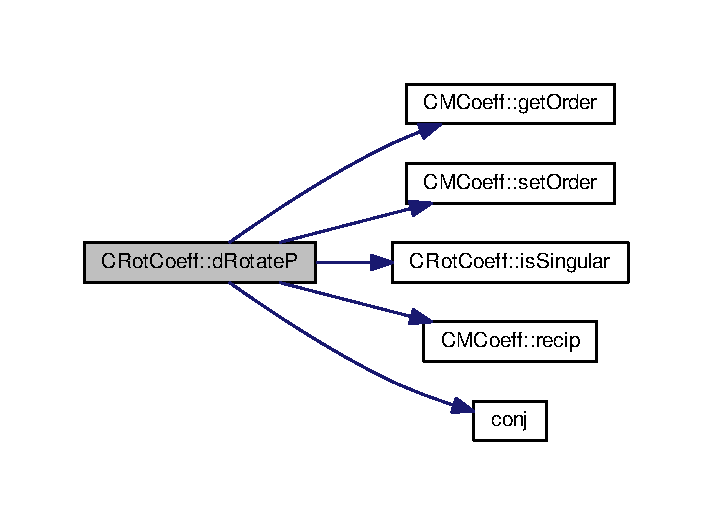
\includegraphics[width=342pt]{classCRotCoeff_a88d3ed40239b588e18399c549509f687_cgraph}
\end{center}
\end{figure}


\hypertarget{classCRotCoeff_a73c21837871db96b643b0e9ccf77a6b4}{\index{C\-Rot\-Coeff@{C\-Rot\-Coeff}!d\-Rotate\-T@{d\-Rotate\-T}}
\index{d\-Rotate\-T@{d\-Rotate\-T}!CRotCoeff@{C\-Rot\-Coeff}}
\subsubsection[{d\-Rotate\-T}]{\setlength{\rightskip}{0pt plus 5cm}void C\-Rot\-Coeff\-::d\-Rotate\-T (
\begin{DoxyParamCaption}
\item[{const {\bf C\-M\-Coeff} \&}]{Min, }
\item[{{\bf C\-M\-Coeff} \&}]{Mout, }
\item[{bool}]{b\-For}
\end{DoxyParamCaption}
)\hspace{0.3cm}{\ttfamily [inline]}}}\label{classCRotCoeff_a73c21837871db96b643b0e9ccf77a6b4}


\hyperlink{classCRotCoeff}{C\-Rot\-Coeff} d\-Rotate\-T function. 

Function to apply the gradient of rotation operator to the M\-P coefficents with respect to T\-H\-E\-T\-A 
\begin{DoxyParams}{Parameters}
{\em Min} & mp coefficient input \\
\hline
{\em Mout} & mp coefficient output \\
\hline
{\em b\-For} & boolean to indicate to compute the original coefficient (true) or the conjugate transpose \\
\hline
\end{DoxyParams}


Here is the call graph for this function\-:\nopagebreak
\begin{figure}[H]
\begin{center}
\leavevmode
\includegraphics[width=190pt]{classCRotCoeff_a73c21837871db96b643b0e9ccf77a6b4_cgraph}
\end{center}
\end{figure}


\hypertarget{classCRotCoeff_ab40b0a7225f78c026e488950545a33d6}{\index{C\-Rot\-Coeff@{C\-Rot\-Coeff}!d\-Rotate\-T@{d\-Rotate\-T}}
\index{d\-Rotate\-T@{d\-Rotate\-T}!CRotCoeff@{C\-Rot\-Coeff}}
\subsubsection[{d\-Rotate\-T}]{\setlength{\rightskip}{0pt plus 5cm}void C\-Rot\-Coeff\-::d\-Rotate\-T (
\begin{DoxyParamCaption}
\item[{const {\bf C\-M\-Coeff} \&}]{Min, }
\item[{{\bf C\-M\-Coeff} \&}]{Mout, }
\item[{int}]{p1, }
\item[{int}]{p2, }
\item[{bool}]{b\-For}
\end{DoxyParamCaption}
)}}\label{classCRotCoeff_ab40b0a7225f78c026e488950545a33d6}


\hyperlink{classCRotCoeff}{C\-Rot\-Coeff} d\-Rotate\-T function. 

Function to apply the gradient of rotation operator to the M\-P coefficents with respect to T\-H\-E\-T\-A 
\begin{DoxyParams}{Parameters}
{\em Min} & mp coefficient input \\
\hline
{\em Mout} & mp coefficient output \\
\hline
{\em p1} & an integer indicating the lowest number of poles \\
\hline
{\em p2} & an integer indicating the highest number of poles \\
\hline
{\em b\-For} & boolean to indicate to compute the original coefficient (true) or the conjugate transpose\\
\hline
\end{DoxyParams}
Apply the derivative of the rotation operator with respect to T\-H\-E\-T\-A to the M\-P coeffs 

Here is the call graph for this function\-:
\nopagebreak
\begin{figure}[H]
\begin{center}
\leavevmode
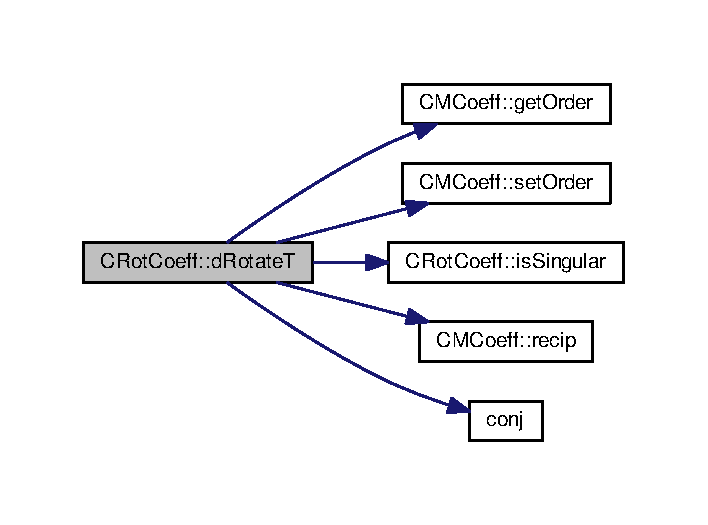
\includegraphics[width=340pt]{classCRotCoeff_ab40b0a7225f78c026e488950545a33d6_cgraph}
\end{center}
\end{figure}


\hypertarget{classCRotCoeff_a27b0198e460737ea20601fa4f0667df5}{\index{C\-Rot\-Coeff@{C\-Rot\-Coeff}!get\-Params@{get\-Params}}
\index{get\-Params@{get\-Params}!CRotCoeff@{C\-Rot\-Coeff}}
\subsubsection[{get\-Params}]{\setlength{\rightskip}{0pt plus 5cm}void C\-Rot\-Coeff\-::get\-Params (
\begin{DoxyParamCaption}
\item[{{\bf R\-E\-A\-L} \&}]{st, }
\item[{{\bf R\-E\-A\-L} \&}]{ct, }
\item[{{\bf R\-E\-A\-L} \&}]{sp, }
\item[{{\bf R\-E\-A\-L} \&}]{cp}
\end{DoxyParamCaption}
) const\hspace{0.3cm}{\ttfamily [inline]}}}\label{classCRotCoeff_a27b0198e460737ea20601fa4f0667df5}
\hypertarget{classCRotCoeff_a1416603a77ab7c9b7af515a7bad684f1}{\index{C\-Rot\-Coeff@{C\-Rot\-Coeff}!inc\-Order@{inc\-Order}}
\index{inc\-Order@{inc\-Order}!CRotCoeff@{C\-Rot\-Coeff}}
\subsubsection[{inc\-Order}]{\setlength{\rightskip}{0pt plus 5cm}void C\-Rot\-Coeff\-::inc\-Order (
\begin{DoxyParamCaption}
{}
\end{DoxyParamCaption}
)}}\label{classCRotCoeff_a1416603a77ab7c9b7af515a7bad684f1}
Function to increase the number of poles and recompute rotation coefficients 

Here is the call graph for this function\-:
\nopagebreak
\begin{figure}[H]
\begin{center}
\leavevmode
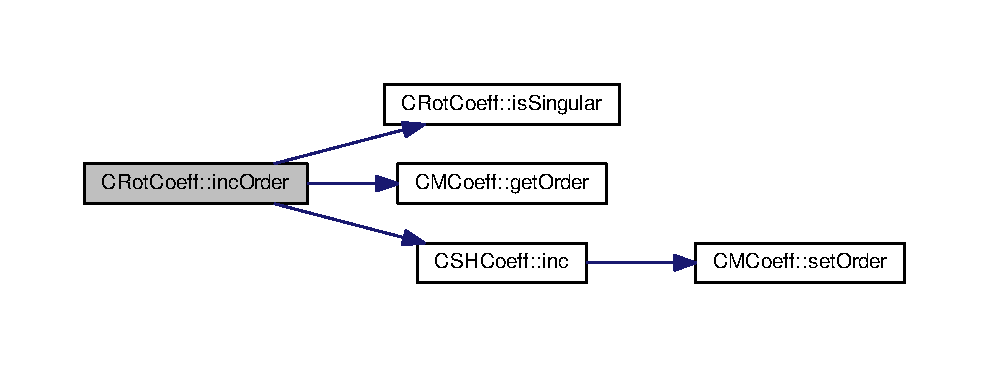
\includegraphics[width=350pt]{classCRotCoeff_a1416603a77ab7c9b7af515a7bad684f1_cgraph}
\end{center}
\end{figure}


\hypertarget{classCRotCoeff_aa51371c84f373916cd8e35031b38cb52}{\index{C\-Rot\-Coeff@{C\-Rot\-Coeff}!init\-Constants@{init\-Constants}}
\index{init\-Constants@{init\-Constants}!CRotCoeff@{C\-Rot\-Coeff}}
\subsubsection[{init\-Constants}]{\setlength{\rightskip}{0pt plus 5cm}void C\-Rot\-Coeff\-::init\-Constants (
\begin{DoxyParamCaption}
{}
\end{DoxyParamCaption}
)\hspace{0.3cm}{\ttfamily [static]}}}\label{classCRotCoeff_aa51371c84f373916cd8e35031b38cb52}


The rotation coefficient init\-Constants function. 

This function initializes the rotation coefficients as described in A.\-1 of Lotan 2006. It initializes a and b constants as described in the appendix. Calls compute\-Q\-Coeff

Initialize the rotation coefficients (includes coeff equs from 2006 paper \hypertarget{classCRotCoeff_a4668070c3eacacf17be98bc2fb348287}{\index{C\-Rot\-Coeff@{C\-Rot\-Coeff}!is\-Singular@{is\-Singular}}
\index{is\-Singular@{is\-Singular}!CRotCoeff@{C\-Rot\-Coeff}}
\subsubsection[{is\-Singular}]{\setlength{\rightskip}{0pt plus 5cm}bool C\-Rot\-Coeff\-::is\-Singular (
\begin{DoxyParamCaption}
{}
\end{DoxyParamCaption}
) const\hspace{0.3cm}{\ttfamily [inline]}}}\label{classCRotCoeff_a4668070c3eacacf17be98bc2fb348287}
\hypertarget{classCRotCoeff_a23dff497ccb1ca53dba01af9a27fdab8}{\index{C\-Rot\-Coeff@{C\-Rot\-Coeff}!outputd\-Rot@{outputd\-Rot}}
\index{outputd\-Rot@{outputd\-Rot}!CRotCoeff@{C\-Rot\-Coeff}}
\subsubsection[{outputd\-Rot}]{\setlength{\rightskip}{0pt plus 5cm}void C\-Rot\-Coeff\-::outputd\-Rot (
\begin{DoxyParamCaption}
\item[{int}]{p}
\end{DoxyParamCaption}
) const}}\label{classCRotCoeff_a23dff497ccb1ca53dba01af9a27fdab8}
Print out derivatives of rot coefficients \hypertarget{classCRotCoeff_a505db8551887fabe49b0f7b6076c2060}{\index{C\-Rot\-Coeff@{C\-Rot\-Coeff}!output\-Rot@{output\-Rot}}
\index{output\-Rot@{output\-Rot}!CRotCoeff@{C\-Rot\-Coeff}}
\subsubsection[{output\-Rot}]{\setlength{\rightskip}{0pt plus 5cm}void C\-Rot\-Coeff\-::output\-Rot (
\begin{DoxyParamCaption}
\item[{int}]{p}
\end{DoxyParamCaption}
) const}}\label{classCRotCoeff_a505db8551887fabe49b0f7b6076c2060}
Print out rotation coefficients \hypertarget{classCRotCoeff_aa52111e9c4cb2949dfae960437742536}{\index{C\-Rot\-Coeff@{C\-Rot\-Coeff}!reset@{reset}}
\index{reset@{reset}!CRotCoeff@{C\-Rot\-Coeff}}
\subsubsection[{reset}]{\setlength{\rightskip}{0pt plus 5cm}void C\-Rot\-Coeff\-::reset (
\begin{DoxyParamCaption}
\item[{{\bf R\-E\-A\-L}}]{theta, }
\item[{{\bf R\-E\-A\-L}}]{phi, }
\item[{{\bf R\-E\-A\-L}}]{xi, }
\item[{int}]{p}
\end{DoxyParamCaption}
)}}\label{classCRotCoeff_aa52111e9c4cb2949dfae960437742536}
reset rotation coefficient given an angle for theta, phi and xi and a number of poles 
\begin{DoxyParams}{Parameters}
{\em theta,a} & real number of angle theta \\
\hline
{\em phi,a} & real number for phi angle in rad \\
\hline
{\em xi} & a \\
\hline
{\em p} & an integer indicating the number of poles \\
\hline
\end{DoxyParams}


Here is the call graph for this function\-:\nopagebreak
\begin{figure}[H]
\begin{center}
\leavevmode
\includegraphics[width=322pt]{classCRotCoeff_aa52111e9c4cb2949dfae960437742536_cgraph}
\end{center}
\end{figure}


\hypertarget{classCRotCoeff_a4a6461f2947e6c07d4a28da4d87a8935}{\index{C\-Rot\-Coeff@{C\-Rot\-Coeff}!reset@{reset}}
\index{reset@{reset}!CRotCoeff@{C\-Rot\-Coeff}}
\subsubsection[{reset}]{\setlength{\rightskip}{0pt plus 5cm}void C\-Rot\-Coeff\-::reset (
\begin{DoxyParamCaption}
\item[{const {\bf C\-Pnt} \&}]{axis, }
\item[{{\bf R\-E\-A\-L}}]{ang, }
\item[{int}]{p}
\end{DoxyParamCaption}
)}}\label{classCRotCoeff_a4a6461f2947e6c07d4a28da4d87a8935}


Here is the call graph for this function\-:\nopagebreak
\begin{figure}[H]
\begin{center}
\leavevmode
\includegraphics[width=350pt]{classCRotCoeff_a4a6461f2947e6c07d4a28da4d87a8935_cgraph}
\end{center}
\end{figure}


\hypertarget{classCRotCoeff_a6dea4a3900cc4ac8c012cc8790b92719}{\index{C\-Rot\-Coeff@{C\-Rot\-Coeff}!reset@{reset}}
\index{reset@{reset}!CRotCoeff@{C\-Rot\-Coeff}}
\subsubsection[{reset}]{\setlength{\rightskip}{0pt plus 5cm}void C\-Rot\-Coeff\-::reset (
\begin{DoxyParamCaption}
\item[{const {\bf C\-Quat} \&}]{Q, }
\item[{int}]{p}
\end{DoxyParamCaption}
)}}\label{classCRotCoeff_a6dea4a3900cc4ac8c012cc8790b92719}
reset\-: Resets the rotation coefficients for a given number of poles 
\begin{DoxyParams}{Parameters}
{\em Q} & a quaternion for rotation \\
\hline
{\em p} & an int describing the number of poles \\
\hline
\end{DoxyParams}


Here is the call graph for this function\-:\nopagebreak
\begin{figure}[H]
\begin{center}
\leavevmode
\includegraphics[width=350pt]{classCRotCoeff_a6dea4a3900cc4ac8c012cc8790b92719_cgraph}
\end{center}
\end{figure}


\hypertarget{classCRotCoeff_aa9b14ebaa2c45a8fa740fa36d9f31d2c}{\index{C\-Rot\-Coeff@{C\-Rot\-Coeff}!rotate@{rotate}}
\index{rotate@{rotate}!CRotCoeff@{C\-Rot\-Coeff}}
\subsubsection[{rotate}]{\setlength{\rightskip}{0pt plus 5cm}void C\-Rot\-Coeff\-::rotate (
\begin{DoxyParamCaption}
\item[{const {\bf C\-Tri\-Coeff} \&}]{Tin, }
\item[{{\bf C\-Tri\-Coeff} \&}]{Tout, }
\item[{bool}]{b\-For}
\end{DoxyParamCaption}
)\hspace{0.3cm}{\ttfamily [inline]}}}\label{classCRotCoeff_aa9b14ebaa2c45a8fa740fa36d9f31d2c}


\hyperlink{classCRotCoeff}{C\-Rot\-Coeff} rotate function. 

Function to apply the rotation operator to the tricoefficents 
\begin{DoxyParams}{Parameters}
{\em Tin} & tri coefficient input \\
\hline
{\em Tout} & tri coefficient output \\
\hline
{\em b\-For} & boolean to indicate to compute the original coefficient or the conjugate transpose \\
\hline
\end{DoxyParams}


Here is the call graph for this function\-:\nopagebreak
\begin{figure}[H]
\begin{center}
\leavevmode
\includegraphics[width=176pt]{classCRotCoeff_aa9b14ebaa2c45a8fa740fa36d9f31d2c_cgraph}
\end{center}
\end{figure}


\hypertarget{classCRotCoeff_a6d65091921f8baa2175c97758dff4e16}{\index{C\-Rot\-Coeff@{C\-Rot\-Coeff}!rotate@{rotate}}
\index{rotate@{rotate}!CRotCoeff@{C\-Rot\-Coeff}}
\subsubsection[{rotate}]{\setlength{\rightskip}{0pt plus 5cm}void C\-Rot\-Coeff\-::rotate (
\begin{DoxyParamCaption}
\item[{const {\bf C\-Tri\-Coeff} \&}]{Tin, }
\item[{{\bf C\-Tri\-Coeff} \&}]{Tout, }
\item[{int}]{p1, }
\item[{int}]{p2, }
\item[{bool}]{b\-For}
\end{DoxyParamCaption}
)\hspace{0.3cm}{\ttfamily [inline]}}}\label{classCRotCoeff_a6d65091921f8baa2175c97758dff4e16}


\hyperlink{classCRotCoeff}{C\-Rot\-Coeff} rotate function. 

\hyperlink{classCRotCoeff}{C\-Rot\-Coeff} rotate.

Function to apply the rotation operator to the tricoefficents 
\begin{DoxyParams}{Parameters}
{\em Tin} & tri coefficient input \\
\hline
{\em Tout} & tri coefficient output \\
\hline
{\em p1} & an integer indicating the lowest number of poles \\
\hline
{\em p2} & an integer indicating the highest number of poles \\
\hline
{\em b\-For} & boolean to indicate to compute the original coefficient (true) or the conjugate transpose\\
\hline
\end{DoxyParams}
Rotate three matrices of tricoeff class 
\begin{DoxyParams}{Parameters}
{\em Tin} & a Tri\-Coeff object for input \\
\hline
{\em Tout} & a Tri\-Coeff object for output \\
\hline
{\em p1} & an int \\
\hline
{\em p2} & an int \\
\hline
{\em b\-For} & a boolean of \\
\hline
\end{DoxyParams}


Here is the call graph for this function\-:\nopagebreak
\begin{figure}[H]
\begin{center}
\leavevmode
\includegraphics[width=308pt]{classCRotCoeff_a6d65091921f8baa2175c97758dff4e16_cgraph}
\end{center}
\end{figure}


\hypertarget{classCRotCoeff_a319c60548de84e430bd55f17d020fa3f}{\index{C\-Rot\-Coeff@{C\-Rot\-Coeff}!rotate@{rotate}}
\index{rotate@{rotate}!CRotCoeff@{C\-Rot\-Coeff}}
\subsubsection[{rotate}]{\setlength{\rightskip}{0pt plus 5cm}void C\-Rot\-Coeff\-::rotate (
\begin{DoxyParamCaption}
\item[{const {\bf C\-M\-Coeff} \&}]{Min, }
\item[{{\bf C\-M\-Coeff} \&}]{Mout, }
\item[{bool}]{b\-For}
\end{DoxyParamCaption}
)\hspace{0.3cm}{\ttfamily [inline]}}}\label{classCRotCoeff_a319c60548de84e430bd55f17d020fa3f}


\hyperlink{classCRotCoeff}{C\-Rot\-Coeff} rotate function. 

Function to apply the rotation operator to the M\-P coefficents 
\begin{DoxyParams}{Parameters}
{\em Min} & mp coefficient input \\
\hline
{\em Mout} & mp coefficient output \\
\hline
{\em b\-For} & boolean to indicate to compute the original coefficient (true) or the conjugate transpose \\
\hline
\end{DoxyParams}


Here is the call graph for this function\-:\nopagebreak
\begin{figure}[H]
\begin{center}
\leavevmode
\includegraphics[width=176pt]{classCRotCoeff_a319c60548de84e430bd55f17d020fa3f_cgraph}
\end{center}
\end{figure}


\hypertarget{classCRotCoeff_ab93dd694803d34505c026b6d48bb6d25}{\index{C\-Rot\-Coeff@{C\-Rot\-Coeff}!rotate@{rotate}}
\index{rotate@{rotate}!CRotCoeff@{C\-Rot\-Coeff}}
\subsubsection[{rotate}]{\setlength{\rightskip}{0pt plus 5cm}void C\-Rot\-Coeff\-::rotate (
\begin{DoxyParamCaption}
\item[{const {\bf C\-M\-Coeff} \&}]{Min, }
\item[{{\bf C\-M\-Coeff} \&}]{Mout, }
\item[{int}]{p1, }
\item[{int}]{p2, }
\item[{bool}]{b\-For}
\end{DoxyParamCaption}
)}}\label{classCRotCoeff_ab93dd694803d34505c026b6d48bb6d25}


\hyperlink{classCRotCoeff}{C\-Rot\-Coeff} rotate function. 

Function to apply the rotation operator to the M\-P coefficents 
\begin{DoxyParams}{Parameters}
{\em Min} & mp coefficient input \\
\hline
{\em Mout} & mp coefficient output \\
\hline
{\em p1} & an integer indicating the lowest number of poles \\
\hline
{\em p2} & an integer indicating the highest number of poles \\
\hline
{\em b\-For} & boolean to indicate to compute the original coefficient (true) or the conjugate transpose\\
\hline
\end{DoxyParams}
Apply the rotation operator to the M\-P coeffs 

Here is the call graph for this function\-:
\nopagebreak
\begin{figure}[H]
\begin{center}
\leavevmode
\includegraphics[width=326pt]{classCRotCoeff_ab93dd694803d34505c026b6d48bb6d25_cgraph}
\end{center}
\end{figure}


\hypertarget{classCRotCoeff_acf2c3650570013fee7e54491fa1d5920}{\index{C\-Rot\-Coeff@{C\-Rot\-Coeff}!save\-Undo@{save\-Undo}}
\index{save\-Undo@{save\-Undo}!CRotCoeff@{C\-Rot\-Coeff}}
\subsubsection[{save\-Undo}]{\setlength{\rightskip}{0pt plus 5cm}void C\-Rot\-Coeff\-::save\-Undo (
\begin{DoxyParamCaption}
{}
\end{DoxyParamCaption}
)\hspace{0.3cm}{\ttfamily [inline]}}}\label{classCRotCoeff_acf2c3650570013fee7e54491fa1d5920}


\hyperlink{classCRotCoeff}{C\-Rot\-Coeff} save\-Undo. 

Save the rotation coefficients and derivatives as an undone move 

Here is the call graph for this function\-:
\nopagebreak
\begin{figure}[H]
\begin{center}
\leavevmode
\includegraphics[width=338pt]{classCRotCoeff_acf2c3650570013fee7e54491fa1d5920_cgraph}
\end{center}
\end{figure}


\hypertarget{classCRotCoeff_a976ea6ff504912701f549e988fd217dc}{\index{C\-Rot\-Coeff@{C\-Rot\-Coeff}!undo@{undo}}
\index{undo@{undo}!CRotCoeff@{C\-Rot\-Coeff}}
\subsubsection[{undo}]{\setlength{\rightskip}{0pt plus 5cm}void C\-Rot\-Coeff\-::undo (
\begin{DoxyParamCaption}
{}
\end{DoxyParamCaption}
)\hspace{0.3cm}{\ttfamily [inline]}}}\label{classCRotCoeff_a976ea6ff504912701f549e988fd217dc}


\hyperlink{classCRotCoeff}{C\-Rot\-Coeff} undo. 

Revert to old rotation coefficients using saved components 

Here is the call graph for this function\-:
\nopagebreak
\begin{figure}[H]
\begin{center}
\leavevmode
\includegraphics[width=292pt]{classCRotCoeff_a976ea6ff504912701f549e988fd217dc_cgraph}
\end{center}
\end{figure}




The documentation for this class was generated from the following files\-:\begin{DoxyCompactItemize}
\item 
\hyperlink{rotcoeff_8h}{rotcoeff.\-h}\item 
\hyperlink{rotcoeff_8cpp}{rotcoeff.\-cpp}\end{DoxyCompactItemize}

\hypertarget{classCSHCoeff}{\section{C\-S\-H\-Coeff Class Reference}
\label{classCSHCoeff}\index{C\-S\-H\-Coeff@{C\-S\-H\-Coeff}}
}


The \hyperlink{classCSHCoeff}{C\-S\-H\-Coeff} class.  




{\ttfamily \#include $<$shcoeff.\-h$>$}



Inheritance diagram for C\-S\-H\-Coeff\-:\nopagebreak
\begin{figure}[H]
\begin{center}
\leavevmode
\includegraphics[width=140pt]{classCSHCoeff__inherit__graph}
\end{center}
\end{figure}


Collaboration diagram for C\-S\-H\-Coeff\-:\nopagebreak
\begin{figure}[H]
\begin{center}
\leavevmode
\includegraphics[width=140pt]{classCSHCoeff__coll__graph}
\end{center}
\end{figure}
\subsection*{Public Member Functions}
\begin{DoxyCompactItemize}
\item 
\hyperlink{classCSHCoeff_a286a374e16fd7741f869fe5edb1ef9d4}{C\-S\-H\-Coeff} (int p=0, int res=\hyperlink{mcoeff_8h_ac23f9c13c5d07d9ce386f7a830c35e5a}{N\-\_\-\-P\-O\-L\-E\-S})
\begin{DoxyCompactList}\small\item\em The \hyperlink{classCSHCoeff}{C\-S\-H\-Coeff} class constructor. \end{DoxyCompactList}\item 
void \hyperlink{classCSHCoeff_a7aa1d16fe8a3e18012f2ccaec89a0a0f}{reset} (\hyperlink{util_8h_a5821460e95a0800cf9f24c38915cbbde}{R\-E\-A\-L} theta, \hyperlink{util_8h_a5821460e95a0800cf9f24c38915cbbde}{R\-E\-A\-L} phi, int p)
\item 
void \hyperlink{classCSHCoeff_adf80cf8370b4db9957de7acfe8aa64d6}{inc} ()
\begin{DoxyCompactList}\small\item\em The \hyperlink{classCSHCoeff}{C\-S\-H\-Coeff} inc function. \end{DoxyCompactList}\end{DoxyCompactItemize}
\subsection*{Static Public Member Functions}
\begin{DoxyCompactItemize}
\item 
static void \hyperlink{classCSHCoeff_ae6ad53fe9a4862de25fe7f2788649a41}{init} (\hyperlink{util_8h_a5821460e95a0800cf9f24c38915cbbde}{R\-E\-A\-L} rs, \hyperlink{util_8h_a5821460e95a0800cf9f24c38915cbbde}{R\-E\-A\-L} kappa)
\item 
static void \hyperlink{classCSHCoeff_acd63e5bb85843c08800a83281f3daad9}{besselk} (\hyperlink{util_8h_a5821460e95a0800cf9f24c38915cbbde}{R\-E\-A\-L} K\mbox{[}$\,$\mbox{]}, int n, \hyperlink{util_8h_a5821460e95a0800cf9f24c38915cbbde}{R\-E\-A\-L} val)
\begin{DoxyCompactList}\small\item\em The \hyperlink{classCSHCoeff}{C\-S\-H\-Coeff} besselk function. \end{DoxyCompactList}\item 
static void \hyperlink{classCSHCoeff_a8fd12308d0884731596cc1268b04d232}{inc\-Besselk} (\hyperlink{util_8h_a5821460e95a0800cf9f24c38915cbbde}{R\-E\-A\-L} K\mbox{[}$\,$\mbox{]}, int p, \hyperlink{util_8h_a5821460e95a0800cf9f24c38915cbbde}{R\-E\-A\-L} val)
\item 
static void \hyperlink{classCSHCoeff_aa6cc07501f3b8ab8d2f9f32ba5a7b279}{besseli} (\hyperlink{util_8h_a5821460e95a0800cf9f24c38915cbbde}{R\-E\-A\-L} I\mbox{[}$\,$\mbox{]}, int n, \hyperlink{util_8h_a5821460e95a0800cf9f24c38915cbbde}{R\-E\-A\-L} val)
\begin{DoxyCompactList}\small\item\em The \hyperlink{classCSHCoeff}{C\-S\-H\-Coeff} besseli function. \end{DoxyCompactList}\item 
static void \hyperlink{classCSHCoeff_ac30535573d45c2da6a424c415967e6f2}{special\-S\-H} (\hyperlink{util_8h_a5821460e95a0800cf9f24c38915cbbde}{R\-E\-A\-L} S\-H\mbox{[}$\,$\mbox{]}, int n, \hyperlink{util_8h_a5821460e95a0800cf9f24c38915cbbde}{R\-E\-A\-L} val)
\end{DoxyCompactItemize}
\subsection*{Additional Inherited Members}


\subsection{Detailed Description}
The \hyperlink{classCSHCoeff}{C\-S\-H\-Coeff} class. 

The \hyperlink{classCSHCoeff}{C\-S\-H\-Coeff} class contains information about spherical harmonics. Contains computations for E\-Q(1) of Lotan 2006 as well as bessel function calculations for equations 2 and 3 

\subsection{Constructor \& Destructor Documentation}
\hypertarget{classCSHCoeff_a286a374e16fd7741f869fe5edb1ef9d4}{\index{C\-S\-H\-Coeff@{C\-S\-H\-Coeff}!C\-S\-H\-Coeff@{C\-S\-H\-Coeff}}
\index{C\-S\-H\-Coeff@{C\-S\-H\-Coeff}!CSHCoeff@{C\-S\-H\-Coeff}}
\subsubsection[{C\-S\-H\-Coeff}]{\setlength{\rightskip}{0pt plus 5cm}C\-S\-H\-Coeff\-::\-C\-S\-H\-Coeff (
\begin{DoxyParamCaption}
\item[{int}]{p = {\ttfamily 0}, }
\item[{int}]{res = {\ttfamily {\bf N\-\_\-\-P\-O\-L\-E\-S}}}
\end{DoxyParamCaption}
)}}\label{classCSHCoeff_a286a374e16fd7741f869fe5edb1ef9d4}


The \hyperlink{classCSHCoeff}{C\-S\-H\-Coeff} class constructor. 

Initialize a \hyperlink{classCSHCoeff}{C\-S\-H\-Coeff} object. 
\begin{DoxyParams}{Parameters}
{\em p} & is an int that is a minimal number of poles. Default is zero. \\
\hline
{\em res} & is an in that describes the total number of residuals (poles) for the expansion. Default is N\-\_\-\-P\-O\-L\-E\-S \\
\hline
\end{DoxyParams}
\begin{DoxyReturn}{Returns}
an object of the \hyperlink{classCSHCoeff}{C\-S\-H\-Coeff} class.
\end{DoxyReturn}
Initialize S\-H\-Coeff class 

\subsection{Member Function Documentation}
\hypertarget{classCSHCoeff_aa6cc07501f3b8ab8d2f9f32ba5a7b279}{\index{C\-S\-H\-Coeff@{C\-S\-H\-Coeff}!besseli@{besseli}}
\index{besseli@{besseli}!CSHCoeff@{C\-S\-H\-Coeff}}
\subsubsection[{besseli}]{\setlength{\rightskip}{0pt plus 5cm}void C\-S\-H\-Coeff\-::besseli (
\begin{DoxyParamCaption}
\item[{{\bf R\-E\-A\-L}}]{I\mbox{[}$\,$\mbox{]}, }
\item[{int}]{n, }
\item[{{\bf R\-E\-A\-L}}]{val}
\end{DoxyParamCaption}
)\hspace{0.3cm}{\ttfamily [static]}}}\label{classCSHCoeff_aa6cc07501f3b8ab8d2f9f32ba5a7b279}


The \hyperlink{classCSHCoeff}{C\-S\-H\-Coeff} besseli function. 

Function to create the i modified spherical bessel function. in(z) = sqrt(pi/(2z)) $\ast$ I n+0.5 (z)

There is a recursion relationship as follows\-: i n+1(z) = (2n+1)$\ast$(2n+3)$\ast$( i n-\/1(z) -\/ i n(z) )/ z$^\wedge$2

But the alternate method used is\-:

i n(z) = 1 + sum\-\_\-(j=1)$^\wedge$\-L t\-\_\-j$^\wedge$n(z$^\wedge$2/2) where\-: t\-\_\-j$^\wedge$n(y) = (1/j)$\ast$t\-\_\-(j-\/1)$^\wedge$n(y)$\ast$(y/(2n+2j+3))


\begin{DoxyParams}{Parameters}
{\em I} & a vector of floating points to store besseli functions of size p \\
\hline
{\em p} & an integer indicating the number of bessel functions to compute \\
\hline
{\em val} & a floating point with the value at which to evaluate the bessel function. Given as z in the Lotan 2006 paper.\\
\hline
\end{DoxyParams}
Function to create the i modified spherical bessel function. \hypertarget{classCSHCoeff_acd63e5bb85843c08800a83281f3daad9}{\index{C\-S\-H\-Coeff@{C\-S\-H\-Coeff}!besselk@{besselk}}
\index{besselk@{besselk}!CSHCoeff@{C\-S\-H\-Coeff}}
\subsubsection[{besselk}]{\setlength{\rightskip}{0pt plus 5cm}void C\-S\-H\-Coeff\-::besselk (
\begin{DoxyParamCaption}
\item[{{\bf R\-E\-A\-L}}]{K\mbox{[}$\,$\mbox{]}, }
\item[{int}]{p, }
\item[{{\bf R\-E\-A\-L}}]{val}
\end{DoxyParamCaption}
)\hspace{0.3cm}{\ttfamily [static]}}}\label{classCSHCoeff_acd63e5bb85843c08800a83281f3daad9}


The \hyperlink{classCSHCoeff}{C\-S\-H\-Coeff} besselk function. 

Function to create the i modified spherical bessel function. kn(z) = sqrt(pi/(2z)) $\ast$ K n+0.5 (z)

There is a recursion relationship as follows\-: k n+1(z) = k n(z) + ( k n-\/1(z) $\ast$ z$^\wedge$2 )/( (2n+1)$\ast$(2n-\/1) )


\begin{DoxyParams}{Parameters}
{\em K} & a vector of floating points to store bessel\-K functions of size p \\
\hline
{\em p} & an integer indicating the number of bessel functions to compute \\
\hline
{\em val} & a floating point with the value at which to evaluate the bessel function. Given as z in the Lotan 2006 paper.\\
\hline
\end{DoxyParams}
Function to create the k modified spherical bessel function. \hypertarget{classCSHCoeff_adf80cf8370b4db9957de7acfe8aa64d6}{\index{C\-S\-H\-Coeff@{C\-S\-H\-Coeff}!inc@{inc}}
\index{inc@{inc}!CSHCoeff@{C\-S\-H\-Coeff}}
\subsubsection[{inc}]{\setlength{\rightskip}{0pt plus 5cm}void C\-S\-H\-Coeff\-::inc (
\begin{DoxyParamCaption}
{}
\end{DoxyParamCaption}
)}}\label{classCSHCoeff_adf80cf8370b4db9957de7acfe8aa64d6}


The \hyperlink{classCSHCoeff}{C\-S\-H\-Coeff} inc function. 

Function to increase S\-H for N\-P\-O\-L\-E\-S=m\-\_\-p+1

Function to increase the number of poles and create a legendre polynomial for m\-\_\-p+1 poles. 

Here is the call graph for this function\-:
\nopagebreak
\begin{figure}[H]
\begin{center}
\leavevmode
\includegraphics[width=298pt]{classCSHCoeff_adf80cf8370b4db9957de7acfe8aa64d6_cgraph}
\end{center}
\end{figure}


\hypertarget{classCSHCoeff_a8fd12308d0884731596cc1268b04d232}{\index{C\-S\-H\-Coeff@{C\-S\-H\-Coeff}!inc\-Besselk@{inc\-Besselk}}
\index{inc\-Besselk@{inc\-Besselk}!CSHCoeff@{C\-S\-H\-Coeff}}
\subsubsection[{inc\-Besselk}]{\setlength{\rightskip}{0pt plus 5cm}void C\-S\-H\-Coeff\-::inc\-Besselk (
\begin{DoxyParamCaption}
\item[{{\bf R\-E\-A\-L}}]{K\mbox{[}$\,$\mbox{]}, }
\item[{int}]{p, }
\item[{{\bf R\-E\-A\-L}}]{val}
\end{DoxyParamCaption}
)\hspace{0.3cm}{\ttfamily [static]}}}\label{classCSHCoeff_a8fd12308d0884731596cc1268b04d232}
Function to increase the stored k modified spherical bessel function \hypertarget{classCSHCoeff_ae6ad53fe9a4862de25fe7f2788649a41}{\index{C\-S\-H\-Coeff@{C\-S\-H\-Coeff}!init@{init}}
\index{init@{init}!CSHCoeff@{C\-S\-H\-Coeff}}
\subsubsection[{init}]{\setlength{\rightskip}{0pt plus 5cm}void C\-S\-H\-Coeff\-::init (
\begin{DoxyParamCaption}
\item[{{\bf R\-E\-A\-L}}]{rs, }
\item[{{\bf R\-E\-A\-L}}]{kappa}
\end{DoxyParamCaption}
)\hspace{0.3cm}{\ttfamily [static]}}}\label{classCSHCoeff_ae6ad53fe9a4862de25fe7f2788649a41}
Initialize the spherical harmonics coefficients Inputs\-: rs = scaling factor $\sim$ avg mol radius in system kappa = inverse debye length \hypertarget{classCSHCoeff_a7aa1d16fe8a3e18012f2ccaec89a0a0f}{\index{C\-S\-H\-Coeff@{C\-S\-H\-Coeff}!reset@{reset}}
\index{reset@{reset}!CSHCoeff@{C\-S\-H\-Coeff}}
\subsubsection[{reset}]{\setlength{\rightskip}{0pt plus 5cm}void C\-S\-H\-Coeff\-::reset (
\begin{DoxyParamCaption}
\item[{{\bf R\-E\-A\-L}}]{theta, }
\item[{{\bf R\-E\-A\-L}}]{phi, }
\item[{int}]{p}
\end{DoxyParamCaption}
)}}\label{classCSHCoeff_a7aa1d16fe8a3e18012f2ccaec89a0a0f}
Reset the spherical harmonics for a given theta and phi 
\begin{DoxyParams}{Parameters}
{\em theta} & a given theta angle for computing S\-H \\
\hline
{\em phi} & a given phi angle for computing S\-H \\
\hline
{\em p} & an int with the number of poles for computing S\-H \\
\hline
\end{DoxyParams}
\hypertarget{classCSHCoeff_ac30535573d45c2da6a424c415967e6f2}{\index{C\-S\-H\-Coeff@{C\-S\-H\-Coeff}!special\-S\-H@{special\-S\-H}}
\index{special\-S\-H@{special\-S\-H}!CSHCoeff@{C\-S\-H\-Coeff}}
\subsubsection[{special\-S\-H}]{\setlength{\rightskip}{0pt plus 5cm}void C\-S\-H\-Coeff\-::special\-S\-H (
\begin{DoxyParamCaption}
\item[{{\bf R\-E\-A\-L}}]{S\-H\mbox{[}$\,$\mbox{]}, }
\item[{int}]{n, }
\item[{{\bf R\-E\-A\-L}}]{val}
\end{DoxyParamCaption}
)\hspace{0.3cm}{\ttfamily [static]}}}\label{classCSHCoeff_ac30535573d45c2da6a424c415967e6f2}
Creating a special spherical harmonic, from a legendre polynomial, using the recursive relationship, for m=1\-: \begin{DoxyVerb}Pl,1 (val) = val * (2l-1)/(l-1) * Pl-1,1(val) - l/(l-1) * Pl-2,1(val)

and finally: SH[l] = -1*sqrt((l-1)!/(l+1)!)*Pl,1(val)\end{DoxyVerb}
 

The documentation for this class was generated from the following files\-:\begin{DoxyCompactItemize}
\item 
\hyperlink{shcoeff_8h}{shcoeff.\-h}\item 
\hyperlink{shcoeff_8cpp}{shcoeff.\-cpp}\end{DoxyCompactItemize}

\hypertarget{classCSpPnt}{\section{C\-Sp\-Pnt Class Reference}
\label{classCSpPnt}\index{C\-Sp\-Pnt@{C\-Sp\-Pnt}}
}


{\ttfamily \#include $<$util.\-h$>$}

\subsection*{Public Member Functions}
\begin{DoxyCompactItemize}
\item 
\hyperlink{classCSpPnt_ab2366cfde717accefce56fc72aa5a2ed}{C\-Sp\-Pnt} ()
\item 
\hyperlink{classCSpPnt_a2d035000bbff43189d79affc0447a9a3}{C\-Sp\-Pnt} (\hyperlink{util_8h_a5821460e95a0800cf9f24c38915cbbde}{R\-E\-A\-L} rho\-\_\-, \hyperlink{util_8h_a5821460e95a0800cf9f24c38915cbbde}{R\-E\-A\-L} theta\-\_\-, \hyperlink{util_8h_a5821460e95a0800cf9f24c38915cbbde}{R\-E\-A\-L} phi\-\_\-)
\item 
const \hyperlink{classCSpPnt}{C\-Sp\-Pnt} \& \hyperlink{classCSpPnt_aee31a3b97c734fa150f1a33daadd6dfc}{operator=} (const \hyperlink{classCSpPnt}{C\-Sp\-Pnt} \&s)
\item 
void \hyperlink{classCSpPnt_a9525366e1c144421d07c0a1485256f82}{zero} ()
\item 
\hyperlink{util_8h_a5821460e95a0800cf9f24c38915cbbde}{R\-E\-A\-L} \& \hyperlink{classCSpPnt_af6364f003b923aa77c880869d27caa64}{rho} ()
\item 
\hyperlink{util_8h_a5821460e95a0800cf9f24c38915cbbde}{R\-E\-A\-L} \& \hyperlink{classCSpPnt_a4b48e7760135fc768ab6911a328194ba}{theta} ()
\item 
\hyperlink{util_8h_a5821460e95a0800cf9f24c38915cbbde}{R\-E\-A\-L} \& \hyperlink{classCSpPnt_af4f411d4a656dfec7c5a69ba065dbe1d}{phi} ()
\item 
const \hyperlink{util_8h_a5821460e95a0800cf9f24c38915cbbde}{R\-E\-A\-L} \hyperlink{classCSpPnt_ad7366f49f0fde0b19a3682ace6b606ba}{rho} () const 
\item 
const \hyperlink{util_8h_a5821460e95a0800cf9f24c38915cbbde}{R\-E\-A\-L} \hyperlink{classCSpPnt_aed72be0c307a800a1b7565ba80d87e1f}{theta} () const 
\item 
const \hyperlink{util_8h_a5821460e95a0800cf9f24c38915cbbde}{R\-E\-A\-L} \hyperlink{classCSpPnt_a4ecdc3162c71e20aed001b40a497a339}{phi} () const 
\end{DoxyCompactItemize}
\subsection*{Friends}
\begin{DoxyCompactItemize}
\item 
ostream \& \hyperlink{classCSpPnt_a53a39a67bc3f52a606be1d4e71085b3f}{operator$<$$<$} (ostream \&out, const \hyperlink{classCSpPnt}{C\-Sp\-Pnt} \&p)
\item 
\hyperlink{classCPnt}{C\-Pnt} \hyperlink{classCSpPnt_af8b263bb80bb3a76271a7f57d5057df3}{Sph\-To\-Cart} (const \hyperlink{classCSpPnt}{C\-Sp\-Pnt} \&s)
\item 
\hyperlink{classCSpPnt}{C\-Sp\-Pnt} \hyperlink{classCSpPnt_ad05fbf75e7550a927bc817f97115f2fc}{Cart\-To\-Sph} (const \hyperlink{classCPnt}{C\-Pnt} \&c)
\end{DoxyCompactItemize}


\subsection{Constructor \& Destructor Documentation}
\hypertarget{classCSpPnt_ab2366cfde717accefce56fc72aa5a2ed}{\index{C\-Sp\-Pnt@{C\-Sp\-Pnt}!C\-Sp\-Pnt@{C\-Sp\-Pnt}}
\index{C\-Sp\-Pnt@{C\-Sp\-Pnt}!CSpPnt@{C\-Sp\-Pnt}}
\subsubsection[{C\-Sp\-Pnt}]{\setlength{\rightskip}{0pt plus 5cm}C\-Sp\-Pnt\-::\-C\-Sp\-Pnt (
\begin{DoxyParamCaption}
{}
\end{DoxyParamCaption}
)\hspace{0.3cm}{\ttfamily [inline]}}}\label{classCSpPnt_ab2366cfde717accefce56fc72aa5a2ed}
\hypertarget{classCSpPnt_a2d035000bbff43189d79affc0447a9a3}{\index{C\-Sp\-Pnt@{C\-Sp\-Pnt}!C\-Sp\-Pnt@{C\-Sp\-Pnt}}
\index{C\-Sp\-Pnt@{C\-Sp\-Pnt}!CSpPnt@{C\-Sp\-Pnt}}
\subsubsection[{C\-Sp\-Pnt}]{\setlength{\rightskip}{0pt plus 5cm}C\-Sp\-Pnt\-::\-C\-Sp\-Pnt (
\begin{DoxyParamCaption}
\item[{{\bf R\-E\-A\-L}}]{rho\-\_\-, }
\item[{{\bf R\-E\-A\-L}}]{theta\-\_\-, }
\item[{{\bf R\-E\-A\-L}}]{phi\-\_\-}
\end{DoxyParamCaption}
)\hspace{0.3cm}{\ttfamily [inline]}}}\label{classCSpPnt_a2d035000bbff43189d79affc0447a9a3}


\subsection{Member Function Documentation}
\hypertarget{classCSpPnt_aee31a3b97c734fa150f1a33daadd6dfc}{\index{C\-Sp\-Pnt@{C\-Sp\-Pnt}!operator=@{operator=}}
\index{operator=@{operator=}!CSpPnt@{C\-Sp\-Pnt}}
\subsubsection[{operator=}]{\setlength{\rightskip}{0pt plus 5cm}const {\bf C\-Sp\-Pnt}\& {\bf C\-Sp\-Pnt\-::operator}= (
\begin{DoxyParamCaption}
\item[{const {\bf C\-Sp\-Pnt} \&}]{s}
\end{DoxyParamCaption}
)\hspace{0.3cm}{\ttfamily [inline]}}}\label{classCSpPnt_aee31a3b97c734fa150f1a33daadd6dfc}


Here is the call graph for this function\-:\nopagebreak
\begin{figure}[H]
\begin{center}
\leavevmode
\includegraphics[width=294pt]{classCSpPnt_aee31a3b97c734fa150f1a33daadd6dfc_cgraph}
\end{center}
\end{figure}


\hypertarget{classCSpPnt_af4f411d4a656dfec7c5a69ba065dbe1d}{\index{C\-Sp\-Pnt@{C\-Sp\-Pnt}!phi@{phi}}
\index{phi@{phi}!CSpPnt@{C\-Sp\-Pnt}}
\subsubsection[{phi}]{\setlength{\rightskip}{0pt plus 5cm}{\bf R\-E\-A\-L}\& C\-Sp\-Pnt\-::phi (
\begin{DoxyParamCaption}
{}
\end{DoxyParamCaption}
)\hspace{0.3cm}{\ttfamily [inline]}}}\label{classCSpPnt_af4f411d4a656dfec7c5a69ba065dbe1d}
\hypertarget{classCSpPnt_a4ecdc3162c71e20aed001b40a497a339}{\index{C\-Sp\-Pnt@{C\-Sp\-Pnt}!phi@{phi}}
\index{phi@{phi}!CSpPnt@{C\-Sp\-Pnt}}
\subsubsection[{phi}]{\setlength{\rightskip}{0pt plus 5cm}const {\bf R\-E\-A\-L} C\-Sp\-Pnt\-::phi (
\begin{DoxyParamCaption}
{}
\end{DoxyParamCaption}
) const\hspace{0.3cm}{\ttfamily [inline]}}}\label{classCSpPnt_a4ecdc3162c71e20aed001b40a497a339}
\hypertarget{classCSpPnt_af6364f003b923aa77c880869d27caa64}{\index{C\-Sp\-Pnt@{C\-Sp\-Pnt}!rho@{rho}}
\index{rho@{rho}!CSpPnt@{C\-Sp\-Pnt}}
\subsubsection[{rho}]{\setlength{\rightskip}{0pt plus 5cm}{\bf R\-E\-A\-L}\& C\-Sp\-Pnt\-::rho (
\begin{DoxyParamCaption}
{}
\end{DoxyParamCaption}
)\hspace{0.3cm}{\ttfamily [inline]}}}\label{classCSpPnt_af6364f003b923aa77c880869d27caa64}
\hypertarget{classCSpPnt_ad7366f49f0fde0b19a3682ace6b606ba}{\index{C\-Sp\-Pnt@{C\-Sp\-Pnt}!rho@{rho}}
\index{rho@{rho}!CSpPnt@{C\-Sp\-Pnt}}
\subsubsection[{rho}]{\setlength{\rightskip}{0pt plus 5cm}const {\bf R\-E\-A\-L} C\-Sp\-Pnt\-::rho (
\begin{DoxyParamCaption}
{}
\end{DoxyParamCaption}
) const\hspace{0.3cm}{\ttfamily [inline]}}}\label{classCSpPnt_ad7366f49f0fde0b19a3682ace6b606ba}
\hypertarget{classCSpPnt_a4b48e7760135fc768ab6911a328194ba}{\index{C\-Sp\-Pnt@{C\-Sp\-Pnt}!theta@{theta}}
\index{theta@{theta}!CSpPnt@{C\-Sp\-Pnt}}
\subsubsection[{theta}]{\setlength{\rightskip}{0pt plus 5cm}{\bf R\-E\-A\-L}\& C\-Sp\-Pnt\-::theta (
\begin{DoxyParamCaption}
{}
\end{DoxyParamCaption}
)\hspace{0.3cm}{\ttfamily [inline]}}}\label{classCSpPnt_a4b48e7760135fc768ab6911a328194ba}
\hypertarget{classCSpPnt_aed72be0c307a800a1b7565ba80d87e1f}{\index{C\-Sp\-Pnt@{C\-Sp\-Pnt}!theta@{theta}}
\index{theta@{theta}!CSpPnt@{C\-Sp\-Pnt}}
\subsubsection[{theta}]{\setlength{\rightskip}{0pt plus 5cm}const {\bf R\-E\-A\-L} C\-Sp\-Pnt\-::theta (
\begin{DoxyParamCaption}
{}
\end{DoxyParamCaption}
) const\hspace{0.3cm}{\ttfamily [inline]}}}\label{classCSpPnt_aed72be0c307a800a1b7565ba80d87e1f}
\hypertarget{classCSpPnt_a9525366e1c144421d07c0a1485256f82}{\index{C\-Sp\-Pnt@{C\-Sp\-Pnt}!zero@{zero}}
\index{zero@{zero}!CSpPnt@{C\-Sp\-Pnt}}
\subsubsection[{zero}]{\setlength{\rightskip}{0pt plus 5cm}void C\-Sp\-Pnt\-::zero (
\begin{DoxyParamCaption}
{}
\end{DoxyParamCaption}
)\hspace{0.3cm}{\ttfamily [inline]}}}\label{classCSpPnt_a9525366e1c144421d07c0a1485256f82}


\subsection{Friends And Related Function Documentation}
\hypertarget{classCSpPnt_ad05fbf75e7550a927bc817f97115f2fc}{\index{C\-Sp\-Pnt@{C\-Sp\-Pnt}!Cart\-To\-Sph@{Cart\-To\-Sph}}
\index{Cart\-To\-Sph@{Cart\-To\-Sph}!CSpPnt@{C\-Sp\-Pnt}}
\subsubsection[{Cart\-To\-Sph}]{\setlength{\rightskip}{0pt plus 5cm}{\bf C\-Sp\-Pnt} Cart\-To\-Sph (
\begin{DoxyParamCaption}
\item[{const {\bf C\-Pnt} \&}]{c}
\end{DoxyParamCaption}
)\hspace{0.3cm}{\ttfamily [friend]}}}\label{classCSpPnt_ad05fbf75e7550a927bc817f97115f2fc}
\hypertarget{classCSpPnt_a53a39a67bc3f52a606be1d4e71085b3f}{\index{C\-Sp\-Pnt@{C\-Sp\-Pnt}!operator$<$$<$@{operator$<$$<$}}
\index{operator$<$$<$@{operator$<$$<$}!CSpPnt@{C\-Sp\-Pnt}}
\subsubsection[{operator$<$$<$}]{\setlength{\rightskip}{0pt plus 5cm}ostream\& {\bf operator}$<$$<$ (
\begin{DoxyParamCaption}
\item[{ostream \&}]{out, }
\item[{const {\bf C\-Sp\-Pnt} \&}]{p}
\end{DoxyParamCaption}
)\hspace{0.3cm}{\ttfamily [friend]}}}\label{classCSpPnt_a53a39a67bc3f52a606be1d4e71085b3f}
\hypertarget{classCSpPnt_af8b263bb80bb3a76271a7f57d5057df3}{\index{C\-Sp\-Pnt@{C\-Sp\-Pnt}!Sph\-To\-Cart@{Sph\-To\-Cart}}
\index{Sph\-To\-Cart@{Sph\-To\-Cart}!CSpPnt@{C\-Sp\-Pnt}}
\subsubsection[{Sph\-To\-Cart}]{\setlength{\rightskip}{0pt plus 5cm}{\bf C\-Pnt} Sph\-To\-Cart (
\begin{DoxyParamCaption}
\item[{const {\bf C\-Sp\-Pnt} \&}]{s}
\end{DoxyParamCaption}
)\hspace{0.3cm}{\ttfamily [friend]}}}\label{classCSpPnt_af8b263bb80bb3a76271a7f57d5057df3}


The documentation for this class was generated from the following file\-:\begin{DoxyCompactItemize}
\item 
\hyperlink{util_8h}{util.\-h}\end{DoxyCompactItemize}

\hypertarget{classCTorqCoeff}{\section{C\-Torq\-Coeff Class Reference}
\label{classCTorqCoeff}\index{C\-Torq\-Coeff@{C\-Torq\-Coeff}}
}


{\ttfamily \#include $<$torqcoeff.\-h$>$}



Inheritance diagram for C\-Torq\-Coeff\-:\nopagebreak
\begin{figure}[H]
\begin{center}
\leavevmode
\includegraphics[width=148pt]{classCTorqCoeff__inherit__graph}
\end{center}
\end{figure}


Collaboration diagram for C\-Torq\-Coeff\-:
\nopagebreak
\begin{figure}[H]
\begin{center}
\leavevmode
\includegraphics[width=148pt]{classCTorqCoeff__coll__graph}
\end{center}
\end{figure}
\subsection*{Public Member Functions}
\begin{DoxyCompactItemize}
\item 
\hyperlink{classCTorqCoeff_a90a2461575ac37a67b70a6b2c3817cf6}{C\-Torq\-Coeff} (int p=0, int res=0)
\item 
\hyperlink{classCTorqCoeff_a247c0abd740c28780ceba265b1201c15}{C\-Torq\-Coeff} (const \hyperlink{classCTriCoeff}{C\-Tri\-Coeff} \&G)
\item 
\hyperlink{classCTorqCoeff_a4c2700efbae3670b13ed1bcea4d990a8}{C\-Torq\-Coeff} (const vector$<$ \hyperlink{util_8h_a5821460e95a0800cf9f24c38915cbbde}{R\-E\-A\-L} $>$ \&charges, const vector$<$ \hyperlink{classCPnt}{C\-Pnt} $>$ \&pos, int p, \hyperlink{util_8h_a5821460e95a0800cf9f24c38915cbbde}{R\-E\-A\-L} rad)
\end{DoxyCompactItemize}
\subsection*{Additional Inherited Members}


\subsection{Constructor \& Destructor Documentation}
\hypertarget{classCTorqCoeff_a90a2461575ac37a67b70a6b2c3817cf6}{\index{C\-Torq\-Coeff@{C\-Torq\-Coeff}!C\-Torq\-Coeff@{C\-Torq\-Coeff}}
\index{C\-Torq\-Coeff@{C\-Torq\-Coeff}!CTorqCoeff@{C\-Torq\-Coeff}}
\subsubsection[{C\-Torq\-Coeff}]{\setlength{\rightskip}{0pt plus 5cm}C\-Torq\-Coeff\-::\-C\-Torq\-Coeff (
\begin{DoxyParamCaption}
\item[{int}]{p = {\ttfamily 0}, }
\item[{int}]{res = {\ttfamily 0}}
\end{DoxyParamCaption}
)\hspace{0.3cm}{\ttfamily [inline]}}}\label{classCTorqCoeff_a90a2461575ac37a67b70a6b2c3817cf6}
\hypertarget{classCTorqCoeff_a247c0abd740c28780ceba265b1201c15}{\index{C\-Torq\-Coeff@{C\-Torq\-Coeff}!C\-Torq\-Coeff@{C\-Torq\-Coeff}}
\index{C\-Torq\-Coeff@{C\-Torq\-Coeff}!CTorqCoeff@{C\-Torq\-Coeff}}
\subsubsection[{C\-Torq\-Coeff}]{\setlength{\rightskip}{0pt plus 5cm}C\-Torq\-Coeff\-::\-C\-Torq\-Coeff (
\begin{DoxyParamCaption}
\item[{const {\bf C\-Tri\-Coeff} \&}]{G}
\end{DoxyParamCaption}
)\hspace{0.3cm}{\ttfamily [inline]}}}\label{classCTorqCoeff_a247c0abd740c28780ceba265b1201c15}
\hypertarget{classCTorqCoeff_a4c2700efbae3670b13ed1bcea4d990a8}{\index{C\-Torq\-Coeff@{C\-Torq\-Coeff}!C\-Torq\-Coeff@{C\-Torq\-Coeff}}
\index{C\-Torq\-Coeff@{C\-Torq\-Coeff}!CTorqCoeff@{C\-Torq\-Coeff}}
\subsubsection[{C\-Torq\-Coeff}]{\setlength{\rightskip}{0pt plus 5cm}C\-Torq\-Coeff\-::\-C\-Torq\-Coeff (
\begin{DoxyParamCaption}
\item[{const vector$<$ {\bf R\-E\-A\-L} $>$ \&}]{charges, }
\item[{const vector$<$ {\bf C\-Pnt} $>$ \&}]{pos, }
\item[{int}]{p, }
\item[{{\bf R\-E\-A\-L}}]{rad}
\end{DoxyParamCaption}
)}}\label{classCTorqCoeff_a4c2700efbae3670b13ed1bcea4d990a8}


Here is the call graph for this function\-:\nopagebreak
\begin{figure}[H]
\begin{center}
\leavevmode
\includegraphics[width=350pt]{classCTorqCoeff_a4c2700efbae3670b13ed1bcea4d990a8_cgraph}
\end{center}
\end{figure}




The documentation for this class was generated from the following files\-:\begin{DoxyCompactItemize}
\item 
\hyperlink{torqcoeff_8h}{torqcoeff.\-h}\item 
\hyperlink{torqcoeff_8cpp}{torqcoeff.\-cpp}\end{DoxyCompactItemize}

\hypertarget{classCTransCoeff}{\section{C\-Trans\-Coeff Class Reference}
\label{classCTransCoeff}\index{C\-Trans\-Coeff@{C\-Trans\-Coeff}}
}


The trans\-Coeff class.  




{\ttfamily \#include $<$transcoeff.\-h$>$}

\subsection*{Public Member Functions}
\begin{DoxyCompactItemize}
\item 
\hyperlink{classCTransCoeff_a1b4eb40fb4a4d8efb14ad684c1a169d4}{C\-Trans\-Coeff} (bool b\-Grad=true)
\begin{DoxyCompactList}\small\item\em The trans\-Coeff class constructor. \end{DoxyCompactList}\item 
void \hyperlink{classCTransCoeff_ade17444acf44e5c80f8caa9a593f03ee}{reset} (\hyperlink{util_8h_a5821460e95a0800cf9f24c38915cbbde}{R\-E\-A\-L} rho, int p)
\begin{DoxyCompactList}\small\item\em Trans\-Coeff reset function. \end{DoxyCompactList}\item 
void \hyperlink{classCTransCoeff_a0152b91eec8d84278e6432019ce4ef91}{translate} (const \hyperlink{classCMCoeff}{C\-M\-Coeff} \&Min, \hyperlink{classCMCoeff}{C\-M\-Coeff} \&Mout, bool tpose)
\begin{DoxyCompactList}\small\item\em Trans\-Coeff translate function. \end{DoxyCompactList}\item 
void \hyperlink{classCTransCoeff_a15c1d9affb86e989dc0beefa0683effb}{translate} (const \hyperlink{classCMCoeff}{C\-M\-Coeff} \&Min, \hyperlink{classCMCoeff}{C\-M\-Coeff} \&Mout, int p, bool tpose)
\begin{DoxyCompactList}\small\item\em Trans\-Coeff translate function. \end{DoxyCompactList}\item 
void \hyperlink{classCTransCoeff_a909121581454680f2b50f797f22715f0}{d\-Translate} (const \hyperlink{classCMCoeff}{C\-M\-Coeff} \&Min, \hyperlink{classCMCoeff}{C\-M\-Coeff} \&Mout, bool tpose)
\begin{DoxyCompactList}\small\item\em Trans\-Coeff d\-Translate function. \end{DoxyCompactList}\item 
void \hyperlink{classCTransCoeff_af1e5496a4734710f04841a202346aefb}{d\-Translate} (const \hyperlink{classCMCoeff}{C\-M\-Coeff} \&Min, \hyperlink{classCMCoeff}{C\-M\-Coeff} \&Mout, int p, bool tpose)
\begin{DoxyCompactList}\small\item\em Trans\-Coeff d\-Translate function. \end{DoxyCompactList}\item 
void \hyperlink{classCTransCoeff_a0b68420a4ae33fc1e8fa3dd00daf413c}{inc\-Translate} (const \hyperlink{classCMCoeff}{C\-M\-Coeff} \&Min, \hyperlink{classCMCoeff}{C\-M\-Coeff} \&Mout, bool tpose)
\begin{DoxyCompactList}\small\item\em Trans\-Coeff d\-Translate function. \end{DoxyCompactList}\item 
\hyperlink{util_8h_a5821460e95a0800cf9f24c38915cbbde}{R\-E\-A\-L} \hyperlink{classCTransCoeff_a9fb52e0afd88150756506af029f86611}{compute\-Error} (const \hyperlink{classCMCoeff}{C\-M\-Coeff} \&t\-M1, const \hyperlink{classCMCoeff}{C\-M\-Coeff} \&t\-M2, int p)
\begin{DoxyCompactList}\small\item\em Trans\-Coeff compute\-Error function. \end{DoxyCompactList}\item 
int \hyperlink{classCTransCoeff_a3c10d7ee9ead85dab5c5d2301cb6bb81}{get\-Order} () const 
\begin{DoxyCompactList}\small\item\em Get the number of poles in the transfer coefficient object. \end{DoxyCompactList}\item 
void \hyperlink{classCTransCoeff_a4148a93440f4f011c4fb8cb26667707e}{inc\-Order} ()
\begin{DoxyCompactList}\small\item\em \hyperlink{classCTransCoeff}{C\-Trans\-Coeff} inc\-Order. \end{DoxyCompactList}\item 
void \hyperlink{classCTransCoeff_a79b28e19c6f8c4a028296b351eb4a30a}{dec\-Order} ()
\begin{DoxyCompactList}\small\item\em \hyperlink{classCTransCoeff}{C\-Trans\-Coeff} dec\-Order. \end{DoxyCompactList}\item 
void \hyperlink{classCTransCoeff_a100c9adb6d3476193842504ddf0a1e99}{output\-Trans} (int p) const 
\item 
void \hyperlink{classCTransCoeff_af80128c89b9785e7d4a0e93702ac523f}{outputd\-Trans} (int p) const 
\item 
void \hyperlink{classCTransCoeff_abdfd0c88d82daed4913df4859087103d}{save\-Undo} ()
\begin{DoxyCompactList}\small\item\em \hyperlink{classCTransCoeff}{C\-Trans\-Coeff} save\-Undo. \end{DoxyCompactList}\item 
void \hyperlink{classCTransCoeff_ac310aa175fd393365941e426e96a290b}{undo} ()
\begin{DoxyCompactList}\small\item\em \hyperlink{classCTransCoeff}{C\-Trans\-Coeff} undo. \end{DoxyCompactList}\item 
void \hyperlink{classCTransCoeff_a16bd5045a9ba639775224cc7f121f4c6}{export\-Mat} (double $\ast$$\ast$T)
\begin{DoxyCompactList}\small\item\em Trans\-Coeff export\-Mat function. \end{DoxyCompactList}\end{DoxyCompactItemize}
\subsection*{Static Public Member Functions}
\begin{DoxyCompactItemize}
\item 
static void \hyperlink{classCTransCoeff_ae4be8ef01d28f5b8d9b4282252575bee}{init\-Constants} ()
\begin{DoxyCompactList}\small\item\em Trans\-Coeff init\-Constants function. \end{DoxyCompactList}\end{DoxyCompactItemize}


\subsection{Detailed Description}
The trans\-Coeff class. 

The class that contains all details for a translation coefficients, as described by the appendix of Lotan 2006. 

\subsection{Constructor \& Destructor Documentation}
\hypertarget{classCTransCoeff_a1b4eb40fb4a4d8efb14ad684c1a169d4}{\index{C\-Trans\-Coeff@{C\-Trans\-Coeff}!C\-Trans\-Coeff@{C\-Trans\-Coeff}}
\index{C\-Trans\-Coeff@{C\-Trans\-Coeff}!CTransCoeff@{C\-Trans\-Coeff}}
\subsubsection[{C\-Trans\-Coeff}]{\setlength{\rightskip}{0pt plus 5cm}C\-Trans\-Coeff\-::\-C\-Trans\-Coeff (
\begin{DoxyParamCaption}
\item[{bool}]{b\-Grad = {\ttfamily true}}
\end{DoxyParamCaption}
)}}\label{classCTransCoeff_a1b4eb40fb4a4d8efb14ad684c1a169d4}


The trans\-Coeff class constructor. 

Constructing a transcoeff class, using input of whether or not to compute the gradient 
\begin{DoxyParams}{Parameters}
{\em b\-Grad} & is a boolean indicating of whether or not to compute gradients the default is yes\\
\hline
\end{DoxyParams}
Constructing a transcoeff class, using input of whether or not to compute the gradient 

\subsection{Member Function Documentation}
\hypertarget{classCTransCoeff_a9fb52e0afd88150756506af029f86611}{\index{C\-Trans\-Coeff@{C\-Trans\-Coeff}!compute\-Error@{compute\-Error}}
\index{compute\-Error@{compute\-Error}!CTransCoeff@{C\-Trans\-Coeff}}
\subsubsection[{compute\-Error}]{\setlength{\rightskip}{0pt plus 5cm}{\bf R\-E\-A\-L} C\-Trans\-Coeff\-::compute\-Error (
\begin{DoxyParamCaption}
\item[{const {\bf C\-M\-Coeff} \&}]{t\-M1, }
\item[{const {\bf C\-M\-Coeff} \&}]{t\-M2, }
\item[{int}]{p}
\end{DoxyParamCaption}
)}}\label{classCTransCoeff_a9fb52e0afd88150756506af029f86611}


Trans\-Coeff compute\-Error function. 

Function to compute the error between two matrix coefficients 
\begin{DoxyParams}{Parameters}
{\em Min} & matrix coefficient input \\
\hline
{\em Mout} & matrix coefficient output \\
\hline
{\em p} & an integer indicating the number of poles\\
\hline
\end{DoxyParams}
compute the error between two matrix coefficients 

Here is the call graph for this function\-:
\nopagebreak
\begin{figure}[H]
\begin{center}
\leavevmode
\includegraphics[width=350pt]{classCTransCoeff_a9fb52e0afd88150756506af029f86611_cgraph}
\end{center}
\end{figure}


\hypertarget{classCTransCoeff_a79b28e19c6f8c4a028296b351eb4a30a}{\index{C\-Trans\-Coeff@{C\-Trans\-Coeff}!dec\-Order@{dec\-Order}}
\index{dec\-Order@{dec\-Order}!CTransCoeff@{C\-Trans\-Coeff}}
\subsubsection[{dec\-Order}]{\setlength{\rightskip}{0pt plus 5cm}void C\-Trans\-Coeff\-::dec\-Order (
\begin{DoxyParamCaption}
{}
\end{DoxyParamCaption}
)\hspace{0.3cm}{\ttfamily [inline]}}}\label{classCTransCoeff_a79b28e19c6f8c4a028296b351eb4a30a}


\hyperlink{classCTransCoeff}{C\-Trans\-Coeff} dec\-Order. 

Decrease the number of poles of the calculation. Memory must be deallocated etc \hypertarget{classCTransCoeff_a909121581454680f2b50f797f22715f0}{\index{C\-Trans\-Coeff@{C\-Trans\-Coeff}!d\-Translate@{d\-Translate}}
\index{d\-Translate@{d\-Translate}!CTransCoeff@{C\-Trans\-Coeff}}
\subsubsection[{d\-Translate}]{\setlength{\rightskip}{0pt plus 5cm}void C\-Trans\-Coeff\-::d\-Translate (
\begin{DoxyParamCaption}
\item[{const {\bf C\-M\-Coeff} \&}]{Min, }
\item[{{\bf C\-M\-Coeff} \&}]{Mout, }
\item[{bool}]{tpose}
\end{DoxyParamCaption}
)\hspace{0.3cm}{\ttfamily [inline]}}}\label{classCTransCoeff_a909121581454680f2b50f797f22715f0}


Trans\-Coeff d\-Translate function. 

Function to apply the derivative tranlation operator to the M\-P coefficents 
\begin{DoxyParams}{Parameters}
{\em Min} & matrix coefficient input \\
\hline
{\em Mout} & matrix coefficient output \\
\hline
{\em tpose} & boolean to indicate whether or not to transpose matrix \\
\hline
\end{DoxyParams}


Here is the call graph for this function\-:\nopagebreak
\begin{figure}[H]
\begin{center}
\leavevmode
\includegraphics[width=206pt]{classCTransCoeff_a909121581454680f2b50f797f22715f0_cgraph}
\end{center}
\end{figure}


\hypertarget{classCTransCoeff_af1e5496a4734710f04841a202346aefb}{\index{C\-Trans\-Coeff@{C\-Trans\-Coeff}!d\-Translate@{d\-Translate}}
\index{d\-Translate@{d\-Translate}!CTransCoeff@{C\-Trans\-Coeff}}
\subsubsection[{d\-Translate}]{\setlength{\rightskip}{0pt plus 5cm}void C\-Trans\-Coeff\-::d\-Translate (
\begin{DoxyParamCaption}
\item[{const {\bf C\-M\-Coeff} \&}]{Min, }
\item[{{\bf C\-M\-Coeff} \&}]{Mout, }
\item[{int}]{p, }
\item[{bool}]{tpose}
\end{DoxyParamCaption}
)}}\label{classCTransCoeff_af1e5496a4734710f04841a202346aefb}


Trans\-Coeff d\-Translate function. 

Function to apply the derivative tranlation operator to the M\-P coefficents 
\begin{DoxyParams}{Parameters}
{\em Min} & matrix coefficient input \\
\hline
{\em Mout} & matrix coefficient output \\
\hline
{\em p} & an integer indicating the number of poles \\
\hline
{\em tpose} & boolean to indicate whether or not to transpose matrix\\
\hline
\end{DoxyParams}
Apply the derivative of the translation operator 

Here is the call graph for this function\-:
\nopagebreak
\begin{figure}[H]
\begin{center}
\leavevmode
\includegraphics[width=342pt]{classCTransCoeff_af1e5496a4734710f04841a202346aefb_cgraph}
\end{center}
\end{figure}


\hypertarget{classCTransCoeff_a16bd5045a9ba639775224cc7f121f4c6}{\index{C\-Trans\-Coeff@{C\-Trans\-Coeff}!export\-Mat@{export\-Mat}}
\index{export\-Mat@{export\-Mat}!CTransCoeff@{C\-Trans\-Coeff}}
\subsubsection[{export\-Mat}]{\setlength{\rightskip}{0pt plus 5cm}void C\-Trans\-Coeff\-::export\-Mat (
\begin{DoxyParamCaption}
\item[{double $\ast$$\ast$}]{T}
\end{DoxyParamCaption}
)}}\label{classCTransCoeff_a16bd5045a9ba639775224cc7f121f4c6}


Trans\-Coeff export\-Mat function. 

Export the translation matrix as a 2\-X2 matrix

Export translation coefficient matrix as 2\-X2 \hypertarget{classCTransCoeff_a3c10d7ee9ead85dab5c5d2301cb6bb81}{\index{C\-Trans\-Coeff@{C\-Trans\-Coeff}!get\-Order@{get\-Order}}
\index{get\-Order@{get\-Order}!CTransCoeff@{C\-Trans\-Coeff}}
\subsubsection[{get\-Order}]{\setlength{\rightskip}{0pt plus 5cm}int C\-Trans\-Coeff\-::get\-Order (
\begin{DoxyParamCaption}
{}
\end{DoxyParamCaption}
) const\hspace{0.3cm}{\ttfamily [inline]}}}\label{classCTransCoeff_a3c10d7ee9ead85dab5c5d2301cb6bb81}


Get the number of poles in the transfer coefficient object. 

\hypertarget{classCTransCoeff_a4148a93440f4f011c4fb8cb26667707e}{\index{C\-Trans\-Coeff@{C\-Trans\-Coeff}!inc\-Order@{inc\-Order}}
\index{inc\-Order@{inc\-Order}!CTransCoeff@{C\-Trans\-Coeff}}
\subsubsection[{inc\-Order}]{\setlength{\rightskip}{0pt plus 5cm}void C\-Trans\-Coeff\-::inc\-Order (
\begin{DoxyParamCaption}
{}
\end{DoxyParamCaption}
)\hspace{0.3cm}{\ttfamily [inline]}}}\label{classCTransCoeff_a4148a93440f4f011c4fb8cb26667707e}


\hyperlink{classCTransCoeff}{C\-Trans\-Coeff} inc\-Order. 

Increase the number of poles of the calculation. Memory must be allocated, the bessel functions increased and the coefficients added too 

Here is the call graph for this function\-:\nopagebreak
\begin{figure}[H]
\begin{center}
\leavevmode
\includegraphics[width=348pt]{classCTransCoeff_a4148a93440f4f011c4fb8cb26667707e_cgraph}
\end{center}
\end{figure}


\hypertarget{classCTransCoeff_a0b68420a4ae33fc1e8fa3dd00daf413c}{\index{C\-Trans\-Coeff@{C\-Trans\-Coeff}!inc\-Translate@{inc\-Translate}}
\index{inc\-Translate@{inc\-Translate}!CTransCoeff@{C\-Trans\-Coeff}}
\subsubsection[{inc\-Translate}]{\setlength{\rightskip}{0pt plus 5cm}void C\-Trans\-Coeff\-::inc\-Translate (
\begin{DoxyParamCaption}
\item[{const {\bf C\-M\-Coeff} \&}]{Min, }
\item[{{\bf C\-M\-Coeff} \&}]{Mout, }
\item[{bool}]{tpose}
\end{DoxyParamCaption}
)}}\label{classCTransCoeff_a0b68420a4ae33fc1e8fa3dd00daf413c}


Trans\-Coeff d\-Translate function. 

Apply the translation operator to transform the top level of M\-P coeeffs assuming translation based upon p-\/1 levels already done. 

Here is the call graph for this function\-:
\nopagebreak
\begin{figure}[H]
\begin{center}
\leavevmode
\includegraphics[width=348pt]{classCTransCoeff_a0b68420a4ae33fc1e8fa3dd00daf413c_cgraph}
\end{center}
\end{figure}


\hypertarget{classCTransCoeff_ae4be8ef01d28f5b8d9b4282252575bee}{\index{C\-Trans\-Coeff@{C\-Trans\-Coeff}!init\-Constants@{init\-Constants}}
\index{init\-Constants@{init\-Constants}!CTransCoeff@{C\-Trans\-Coeff}}
\subsubsection[{init\-Constants}]{\setlength{\rightskip}{0pt plus 5cm}void C\-Trans\-Coeff\-::init\-Constants (
\begin{DoxyParamCaption}
{}
\end{DoxyParamCaption}
)\hspace{0.3cm}{\ttfamily [static]}}}\label{classCTransCoeff_ae4be8ef01d28f5b8d9b4282252575bee}


Trans\-Coeff init\-Constants function. 

Function to initialize constants used in trans. coeff recursion

Initialize the rotation coefficients (includes coeff equs from 2006 paper \hypertarget{classCTransCoeff_af80128c89b9785e7d4a0e93702ac523f}{\index{C\-Trans\-Coeff@{C\-Trans\-Coeff}!outputd\-Trans@{outputd\-Trans}}
\index{outputd\-Trans@{outputd\-Trans}!CTransCoeff@{C\-Trans\-Coeff}}
\subsubsection[{outputd\-Trans}]{\setlength{\rightskip}{0pt plus 5cm}void C\-Trans\-Coeff\-::outputd\-Trans (
\begin{DoxyParamCaption}
\item[{int}]{p}
\end{DoxyParamCaption}
) const}}\label{classCTransCoeff_af80128c89b9785e7d4a0e93702ac523f}
Print out derivatives of trans coefficients \hypertarget{classCTransCoeff_a100c9adb6d3476193842504ddf0a1e99}{\index{C\-Trans\-Coeff@{C\-Trans\-Coeff}!output\-Trans@{output\-Trans}}
\index{output\-Trans@{output\-Trans}!CTransCoeff@{C\-Trans\-Coeff}}
\subsubsection[{output\-Trans}]{\setlength{\rightskip}{0pt plus 5cm}void C\-Trans\-Coeff\-::output\-Trans (
\begin{DoxyParamCaption}
\item[{int}]{p}
\end{DoxyParamCaption}
) const}}\label{classCTransCoeff_a100c9adb6d3476193842504ddf0a1e99}
Print out trans coefficients \hypertarget{classCTransCoeff_ade17444acf44e5c80f8caa9a593f03ee}{\index{C\-Trans\-Coeff@{C\-Trans\-Coeff}!reset@{reset}}
\index{reset@{reset}!CTransCoeff@{C\-Trans\-Coeff}}
\subsubsection[{reset}]{\setlength{\rightskip}{0pt plus 5cm}void C\-Trans\-Coeff\-::reset (
\begin{DoxyParamCaption}
\item[{{\bf R\-E\-A\-L}}]{rho, }
\item[{int}]{p}
\end{DoxyParamCaption}
)}}\label{classCTransCoeff_ade17444acf44e5c80f8caa9a593f03ee}


Trans\-Coeff reset function. 

Function to reset the translation coefficients and reallocate space 
\begin{DoxyParams}{Parameters}
{\em rho} & a floating point with the new desired distance, d \\
\hline
{\em p} & an int containing the new number of poles\\
\hline
\end{DoxyParams}
Reset distance, poles, and memory \hypertarget{classCTransCoeff_abdfd0c88d82daed4913df4859087103d}{\index{C\-Trans\-Coeff@{C\-Trans\-Coeff}!save\-Undo@{save\-Undo}}
\index{save\-Undo@{save\-Undo}!CTransCoeff@{C\-Trans\-Coeff}}
\subsubsection[{save\-Undo}]{\setlength{\rightskip}{0pt plus 5cm}void C\-Trans\-Coeff\-::save\-Undo (
\begin{DoxyParamCaption}
{}
\end{DoxyParamCaption}
)\hspace{0.3cm}{\ttfamily [inline]}}}\label{classCTransCoeff_abdfd0c88d82daed4913df4859087103d}


\hyperlink{classCTransCoeff}{C\-Trans\-Coeff} save\-Undo. 

Save the translation coefficients and derivatives as an undone move \hypertarget{classCTransCoeff_a0152b91eec8d84278e6432019ce4ef91}{\index{C\-Trans\-Coeff@{C\-Trans\-Coeff}!translate@{translate}}
\index{translate@{translate}!CTransCoeff@{C\-Trans\-Coeff}}
\subsubsection[{translate}]{\setlength{\rightskip}{0pt plus 5cm}void C\-Trans\-Coeff\-::translate (
\begin{DoxyParamCaption}
\item[{const {\bf C\-M\-Coeff} \&}]{Min, }
\item[{{\bf C\-M\-Coeff} \&}]{Mout, }
\item[{bool}]{tpose}
\end{DoxyParamCaption}
)\hspace{0.3cm}{\ttfamily [inline]}}}\label{classCTransCoeff_a0152b91eec8d84278e6432019ce4ef91}


Trans\-Coeff translate function. 

Function to apply the tranlation operator to the M\-P coefficents 
\begin{DoxyParams}{Parameters}
{\em Min} & matrix coefficient input \\
\hline
{\em Mout} & matrix coefficient output \\
\hline
{\em tpose} & boolean to indicate whether or not to transpose matrix \\
\hline
\end{DoxyParams}


Here is the call graph for this function\-:\nopagebreak
\begin{figure}[H]
\begin{center}
\leavevmode
\includegraphics[width=196pt]{classCTransCoeff_a0152b91eec8d84278e6432019ce4ef91_cgraph}
\end{center}
\end{figure}


\hypertarget{classCTransCoeff_a15c1d9affb86e989dc0beefa0683effb}{\index{C\-Trans\-Coeff@{C\-Trans\-Coeff}!translate@{translate}}
\index{translate@{translate}!CTransCoeff@{C\-Trans\-Coeff}}
\subsubsection[{translate}]{\setlength{\rightskip}{0pt plus 5cm}void C\-Trans\-Coeff\-::translate (
\begin{DoxyParamCaption}
\item[{const {\bf C\-M\-Coeff} \&}]{Min, }
\item[{{\bf C\-M\-Coeff} \&}]{Mout, }
\item[{int}]{p, }
\item[{bool}]{tpose}
\end{DoxyParamCaption}
)}}\label{classCTransCoeff_a15c1d9affb86e989dc0beefa0683effb}


Trans\-Coeff translate function. 

Function to apply the tranlation operator to the M\-P coefficents 
\begin{DoxyParams}{Parameters}
{\em Min} & matrix coefficient input \\
\hline
{\em Mout} & matrix coefficient output \\
\hline
{\em p} & an integer indicating the number of poles \\
\hline
{\em tpose} & boolean to indicate whether or not to transpose matrix\\
\hline
\end{DoxyParams}
Apply the translation operator to the M\-P coeffs 

Here is the call graph for this function\-:
\nopagebreak
\begin{figure}[H]
\begin{center}
\leavevmode
\includegraphics[width=332pt]{classCTransCoeff_a15c1d9affb86e989dc0beefa0683effb_cgraph}
\end{center}
\end{figure}


\hypertarget{classCTransCoeff_ac310aa175fd393365941e426e96a290b}{\index{C\-Trans\-Coeff@{C\-Trans\-Coeff}!undo@{undo}}
\index{undo@{undo}!CTransCoeff@{C\-Trans\-Coeff}}
\subsubsection[{undo}]{\setlength{\rightskip}{0pt plus 5cm}void C\-Trans\-Coeff\-::undo (
\begin{DoxyParamCaption}
{}
\end{DoxyParamCaption}
)\hspace{0.3cm}{\ttfamily [inline]}}}\label{classCTransCoeff_ac310aa175fd393365941e426e96a290b}


\hyperlink{classCTransCoeff}{C\-Trans\-Coeff} undo. 

Revert to old tranlation coefficients using saved components 

The documentation for this class was generated from the following files\-:\begin{DoxyCompactItemize}
\item 
\hyperlink{transcoeff_8h}{transcoeff.\-h}\item 
\hyperlink{transcoeff_8cpp}{transcoeff.\-cpp}\end{DoxyCompactItemize}

\hypertarget{classCTriCoeff}{\section{C\-Tri\-Coeff Class Reference}
\label{classCTriCoeff}\index{C\-Tri\-Coeff@{C\-Tri\-Coeff}}
}


{\ttfamily \#include $<$tricoeff.\-h$>$}



Inheritance diagram for C\-Tri\-Coeff\-:
\nopagebreak
\begin{figure}[H]
\begin{center}
\leavevmode
\includegraphics[width=235pt]{classCTriCoeff__inherit__graph}
\end{center}
\end{figure}


Collaboration diagram for C\-Tri\-Coeff\-:
\nopagebreak
\begin{figure}[H]
\begin{center}
\leavevmode
\includegraphics[width=138pt]{classCTriCoeff__coll__graph}
\end{center}
\end{figure}
\subsection*{Public Member Functions}
\begin{DoxyCompactItemize}
\item 
\hyperlink{classCTriCoeff_a00b825a596e5f4dd0184a50c53bd5d3c}{C\-Tri\-Coeff} (int p=0, int res=\hyperlink{mcoeff_8h_ac23f9c13c5d07d9ce386f7a830c35e5a}{N\-\_\-\-P\-O\-L\-E\-S})
\item 
\hyperlink{classCTriCoeff_ad086149d1a3911a29aeef3dd14ed4042}{C\-Tri\-Coeff} (const \hyperlink{classCTriCoeff}{C\-Tri\-Coeff} \&G)
\item 
const \hyperlink{classCTriCoeff}{C\-Tri\-Coeff} \& \hyperlink{classCTriCoeff_a303a152b75ea66fcd65f5377b317b4d1}{operator=} (const \hyperlink{classCTriCoeff}{C\-Tri\-Coeff} \&G)
\item 
void \hyperlink{classCTriCoeff_ae0b9dd50b8bef198ddd02ba8027d11a3}{copy} (const \hyperlink{classCTriCoeff}{C\-Tri\-Coeff} \&G, int p)
\item 
void \hyperlink{classCTriCoeff_a6568774c5e5a6fe066c739a718de1ba6}{copy\-\_\-p} (const \hyperlink{classCTriCoeff}{C\-Tri\-Coeff} \&G, int p)
\item 
void \hyperlink{classCTriCoeff_aa80c22419286d9fc99daafb90a44d03e}{rotate} (const \hyperlink{classCQuat}{C\-Quat} \&Q, int p)
\item 
void \hyperlink{classCTriCoeff_a2c13fdad1377155cfa7123f8bd04a634}{inc\-Rotate} (const \hyperlink{classCQuat}{C\-Quat} \&Q)
\item 
void \hyperlink{classCTriCoeff_ada2ca53b0a0e3f6b8c9667fd7984e610}{reset} (int p=0)
\item 
void \hyperlink{classCTriCoeff_a0cd79d07cd4eb27e673886611f94f3ab}{recip} ()
\item 
\hyperlink{classCTriCoeff}{C\-Tri\-Coeff} \& \hyperlink{classCTriCoeff_aef9fe1d38095a8764a1d65117c1ca10a}{operator+=} (const \hyperlink{classCTriCoeff}{C\-Tri\-Coeff} \&E)
\item 
\hyperlink{classCTriCoeff}{C\-Tri\-Coeff} \& \hyperlink{classCTriCoeff_a6b15143e57034f33f5e1a716d995ff95}{operator-\/=} (const \hyperlink{classCTriCoeff}{C\-Tri\-Coeff} \&E)
\item 
\hyperlink{classCTriCoeff}{C\-Tri\-Coeff} \& \hyperlink{classCTriCoeff_aec9e2fe8be849b6dfbcfd962c45c1695}{operator$\ast$=} (const \hyperlink{util_8h_a5821460e95a0800cf9f24c38915cbbde}{R\-E\-A\-L} $\ast$C)
\item 
int \hyperlink{classCTriCoeff_a0190ac9feab5bb2cb5e04ea48539b2fe}{get\-Order} () const 
\item 
void \hyperlink{classCTriCoeff_a8df569d14c28af368916f6d6258faa35}{set\-Order} (int p)
\item 
const \hyperlink{classCMCoeff}{C\-M\-Coeff} \& \hyperlink{classCTriCoeff_ae1643fb9444f997935013aeef30a7c1e}{operator\mbox{[}$\,$\mbox{]}} (int c) const 
\item 
\hyperlink{classCMCoeff}{C\-M\-Coeff} \& \hyperlink{classCTriCoeff_ad336c1bb46a865f0543c13ec3bf10557}{operator\mbox{[}$\,$\mbox{]}} (int c)
\item 
virtual void \hyperlink{classCTriCoeff_ad4c1064a7de4dd89f81959d842812ee2}{output} () const 
\item 
void \hyperlink{classCTriCoeff_a9886af4188561152d331366cfaec1c53}{save\-Undo} ()
\item 
void \hyperlink{classCTriCoeff_a8202256093cb071f6ae95887ea1c8dde}{undo} ()
\end{DoxyCompactItemize}
\subsection*{Static Public Member Functions}
\begin{DoxyCompactItemize}
\item 
static \hyperlink{util_8h_a5821460e95a0800cf9f24c38915cbbde}{R\-E\-A\-L} \hyperlink{classCTriCoeff_a5966b12dbe81e9e50f5397647cb18044}{compute\-Dev} (const \hyperlink{classCTriCoeff}{C\-Tri\-Coeff} \&G1, const \hyperlink{classCTriCoeff}{C\-Tri\-Coeff} \&G2)
\end{DoxyCompactItemize}
\subsection*{Protected Attributes}
\begin{DoxyCompactItemize}
\item 
\hyperlink{classCMCoeff}{C\-M\-Coeff} \hyperlink{classCTriCoeff_afac3ecb3b5c965a7ba4cc0409c2100e8}{m\-\_\-\-M} \mbox{[}3\mbox{]}
\end{DoxyCompactItemize}
\subsection*{Friends}
\begin{DoxyCompactItemize}
\item 
\hyperlink{classCTriCoeff}{C\-Tri\-Coeff} \hyperlink{classCTriCoeff_a8684b78e6ecaae7dfa436ee9f52365dd}{operator$\ast$} (const \hyperlink{classCTriCoeff}{C\-Tri\-Coeff} \&G, const \hyperlink{util_8h_a5821460e95a0800cf9f24c38915cbbde}{R\-E\-A\-L} C\mbox{[}\hyperlink{mcoeff_8h_ac23f9c13c5d07d9ce386f7a830c35e5a}{N\-\_\-\-P\-O\-L\-E\-S}\mbox{]})
\item 
\hyperlink{classCTriCoeff}{C\-Tri\-Coeff} \hyperlink{classCTriCoeff_a6678a29fe9fa9c5d7616a7151866fd4c}{operator+} (const \hyperlink{classCTriCoeff}{C\-Tri\-Coeff} \&G1, const \hyperlink{classCTriCoeff}{C\-Tri\-Coeff} \&G2)
\item 
\hyperlink{classCTriCoeff}{C\-Tri\-Coeff} \hyperlink{classCTriCoeff_a6849759bb53453f535b3b2e9379ef7d2}{operator-\/} (const \hyperlink{classCTriCoeff}{C\-Tri\-Coeff} \&G1, const \hyperlink{classCTriCoeff}{C\-Tri\-Coeff} \&G2)
\item 
\hyperlink{classCPnt}{C\-Pnt} \hyperlink{classCTriCoeff_ab5e8aeefc06a5962699ac639820d77be}{cross} (const \hyperlink{classCTriCoeff}{C\-Tri\-Coeff} \&G1, const \hyperlink{classCTriCoeff}{C\-Tri\-Coeff} \&G2)
\item 
\hyperlink{classCPnt}{C\-Pnt} \hyperlink{classCTriCoeff_a095588ecdb857546a57e3f8f33ec983d}{inprod} (const \hyperlink{classCMCoeff}{C\-M\-Coeff} \&M1, const \hyperlink{classCTriCoeff}{C\-Tri\-Coeff} \&M2)
\item 
ostream \& \hyperlink{classCTriCoeff_a47cfb1958c5a43e847aa4e45e1c2c5d4}{operator$<$$<$} (ostream \&out, const \hyperlink{classCTriCoeff}{C\-Tri\-Coeff} \&exp)
\item 
\hyperlink{classCTriCoeff}{C\-Tri\-Coeff} \hyperlink{classCTriCoeff_a66ea424a347d0a78069536bf701393a5}{conj} (const \hyperlink{classCTriCoeff}{C\-Tri\-Coeff} \&G)
\end{DoxyCompactItemize}


\subsection{Constructor \& Destructor Documentation}
\hypertarget{classCTriCoeff_a00b825a596e5f4dd0184a50c53bd5d3c}{\index{C\-Tri\-Coeff@{C\-Tri\-Coeff}!C\-Tri\-Coeff@{C\-Tri\-Coeff}}
\index{C\-Tri\-Coeff@{C\-Tri\-Coeff}!CTriCoeff@{C\-Tri\-Coeff}}
\subsubsection[{C\-Tri\-Coeff}]{\setlength{\rightskip}{0pt plus 5cm}C\-Tri\-Coeff\-::\-C\-Tri\-Coeff (
\begin{DoxyParamCaption}
\item[{int}]{p = {\ttfamily 0}, }
\item[{int}]{res = {\ttfamily {\bf N\-\_\-\-P\-O\-L\-E\-S}}}
\end{DoxyParamCaption}
)}}\label{classCTriCoeff_a00b825a596e5f4dd0184a50c53bd5d3c}


Here is the call graph for this function\-:
\nopagebreak
\begin{figure}[H]
\begin{center}
\leavevmode
\includegraphics[width=320pt]{classCTriCoeff_a00b825a596e5f4dd0184a50c53bd5d3c_cgraph}
\end{center}
\end{figure}


\hypertarget{classCTriCoeff_ad086149d1a3911a29aeef3dd14ed4042}{\index{C\-Tri\-Coeff@{C\-Tri\-Coeff}!C\-Tri\-Coeff@{C\-Tri\-Coeff}}
\index{C\-Tri\-Coeff@{C\-Tri\-Coeff}!CTriCoeff@{C\-Tri\-Coeff}}
\subsubsection[{C\-Tri\-Coeff}]{\setlength{\rightskip}{0pt plus 5cm}C\-Tri\-Coeff\-::\-C\-Tri\-Coeff (
\begin{DoxyParamCaption}
\item[{const {\bf C\-Tri\-Coeff} \&}]{G}
\end{DoxyParamCaption}
)\hspace{0.3cm}{\ttfamily [inline]}}}\label{classCTriCoeff_ad086149d1a3911a29aeef3dd14ed4042}


\subsection{Member Function Documentation}
\hypertarget{classCTriCoeff_a5966b12dbe81e9e50f5397647cb18044}{\index{C\-Tri\-Coeff@{C\-Tri\-Coeff}!compute\-Dev@{compute\-Dev}}
\index{compute\-Dev@{compute\-Dev}!CTriCoeff@{C\-Tri\-Coeff}}
\subsubsection[{compute\-Dev}]{\setlength{\rightskip}{0pt plus 5cm}{\bf R\-E\-A\-L} C\-Tri\-Coeff\-::compute\-Dev (
\begin{DoxyParamCaption}
\item[{const {\bf C\-Tri\-Coeff} \&}]{G1, }
\item[{const {\bf C\-Tri\-Coeff} \&}]{G2}
\end{DoxyParamCaption}
)\hspace{0.3cm}{\ttfamily [inline]}, {\ttfamily [static]}}}\label{classCTriCoeff_a5966b12dbe81e9e50f5397647cb18044}


Here is the call graph for this function\-:
\nopagebreak
\begin{figure}[H]
\begin{center}
\leavevmode
\includegraphics[width=350pt]{classCTriCoeff_a5966b12dbe81e9e50f5397647cb18044_cgraph}
\end{center}
\end{figure}


\hypertarget{classCTriCoeff_ae0b9dd50b8bef198ddd02ba8027d11a3}{\index{C\-Tri\-Coeff@{C\-Tri\-Coeff}!copy@{copy}}
\index{copy@{copy}!CTriCoeff@{C\-Tri\-Coeff}}
\subsubsection[{copy}]{\setlength{\rightskip}{0pt plus 5cm}void C\-Tri\-Coeff\-::copy (
\begin{DoxyParamCaption}
\item[{const {\bf C\-Tri\-Coeff} \&}]{G, }
\item[{int}]{p}
\end{DoxyParamCaption}
)\hspace{0.3cm}{\ttfamily [inline]}}}\label{classCTriCoeff_ae0b9dd50b8bef198ddd02ba8027d11a3}
\hypertarget{classCTriCoeff_a6568774c5e5a6fe066c739a718de1ba6}{\index{C\-Tri\-Coeff@{C\-Tri\-Coeff}!copy\-\_\-p@{copy\-\_\-p}}
\index{copy\-\_\-p@{copy\-\_\-p}!CTriCoeff@{C\-Tri\-Coeff}}
\subsubsection[{copy\-\_\-p}]{\setlength{\rightskip}{0pt plus 5cm}void C\-Tri\-Coeff\-::copy\-\_\-p (
\begin{DoxyParamCaption}
\item[{const {\bf C\-Tri\-Coeff} \&}]{G, }
\item[{int}]{p}
\end{DoxyParamCaption}
)\hspace{0.3cm}{\ttfamily [inline]}}}\label{classCTriCoeff_a6568774c5e5a6fe066c739a718de1ba6}
\hypertarget{classCTriCoeff_a0190ac9feab5bb2cb5e04ea48539b2fe}{\index{C\-Tri\-Coeff@{C\-Tri\-Coeff}!get\-Order@{get\-Order}}
\index{get\-Order@{get\-Order}!CTriCoeff@{C\-Tri\-Coeff}}
\subsubsection[{get\-Order}]{\setlength{\rightskip}{0pt plus 5cm}int C\-Tri\-Coeff\-::get\-Order (
\begin{DoxyParamCaption}
{}
\end{DoxyParamCaption}
) const\hspace{0.3cm}{\ttfamily [inline]}}}\label{classCTriCoeff_a0190ac9feab5bb2cb5e04ea48539b2fe}
\hypertarget{classCTriCoeff_a2c13fdad1377155cfa7123f8bd04a634}{\index{C\-Tri\-Coeff@{C\-Tri\-Coeff}!inc\-Rotate@{inc\-Rotate}}
\index{inc\-Rotate@{inc\-Rotate}!CTriCoeff@{C\-Tri\-Coeff}}
\subsubsection[{inc\-Rotate}]{\setlength{\rightskip}{0pt plus 5cm}void C\-Tri\-Coeff\-::inc\-Rotate (
\begin{DoxyParamCaption}
\item[{const {\bf C\-Quat} \&}]{Q}
\end{DoxyParamCaption}
)}}\label{classCTriCoeff_a2c13fdad1377155cfa7123f8bd04a634}


Here is the call graph for this function\-:
\nopagebreak
\begin{figure}[H]
\begin{center}
\leavevmode
\includegraphics[width=328pt]{classCTriCoeff_a2c13fdad1377155cfa7123f8bd04a634_cgraph}
\end{center}
\end{figure}


\hypertarget{classCTriCoeff_aec9e2fe8be849b6dfbcfd962c45c1695}{\index{C\-Tri\-Coeff@{C\-Tri\-Coeff}!operator$\ast$=@{operator$\ast$=}}
\index{operator$\ast$=@{operator$\ast$=}!CTriCoeff@{C\-Tri\-Coeff}}
\subsubsection[{operator$\ast$=}]{\setlength{\rightskip}{0pt plus 5cm}{\bf C\-Tri\-Coeff}\& {\bf C\-Tri\-Coeff\-::operator}$\ast$= (
\begin{DoxyParamCaption}
\item[{const {\bf R\-E\-A\-L} $\ast$}]{C}
\end{DoxyParamCaption}
)\hspace{0.3cm}{\ttfamily [inline]}}}\label{classCTriCoeff_aec9e2fe8be849b6dfbcfd962c45c1695}
\hypertarget{classCTriCoeff_aef9fe1d38095a8764a1d65117c1ca10a}{\index{C\-Tri\-Coeff@{C\-Tri\-Coeff}!operator+=@{operator+=}}
\index{operator+=@{operator+=}!CTriCoeff@{C\-Tri\-Coeff}}
\subsubsection[{operator+=}]{\setlength{\rightskip}{0pt plus 5cm}{\bf C\-Tri\-Coeff}\& {\bf C\-Tri\-Coeff\-::operator}+= (
\begin{DoxyParamCaption}
\item[{const {\bf C\-Tri\-Coeff} \&}]{E}
\end{DoxyParamCaption}
)\hspace{0.3cm}{\ttfamily [inline]}}}\label{classCTriCoeff_aef9fe1d38095a8764a1d65117c1ca10a}
\hypertarget{classCTriCoeff_a6b15143e57034f33f5e1a716d995ff95}{\index{C\-Tri\-Coeff@{C\-Tri\-Coeff}!operator-\/=@{operator-\/=}}
\index{operator-\/=@{operator-\/=}!CTriCoeff@{C\-Tri\-Coeff}}
\subsubsection[{operator-\/=}]{\setlength{\rightskip}{0pt plus 5cm}{\bf C\-Tri\-Coeff}\& {\bf C\-Tri\-Coeff\-::operator}-\/= (
\begin{DoxyParamCaption}
\item[{const {\bf C\-Tri\-Coeff} \&}]{E}
\end{DoxyParamCaption}
)\hspace{0.3cm}{\ttfamily [inline]}}}\label{classCTriCoeff_a6b15143e57034f33f5e1a716d995ff95}
\hypertarget{classCTriCoeff_a303a152b75ea66fcd65f5377b317b4d1}{\index{C\-Tri\-Coeff@{C\-Tri\-Coeff}!operator=@{operator=}}
\index{operator=@{operator=}!CTriCoeff@{C\-Tri\-Coeff}}
\subsubsection[{operator=}]{\setlength{\rightskip}{0pt plus 5cm}const {\bf C\-Tri\-Coeff}\& {\bf C\-Tri\-Coeff\-::operator}= (
\begin{DoxyParamCaption}
\item[{const {\bf C\-Tri\-Coeff} \&}]{G}
\end{DoxyParamCaption}
)\hspace{0.3cm}{\ttfamily [inline]}}}\label{classCTriCoeff_a303a152b75ea66fcd65f5377b317b4d1}
\hypertarget{classCTriCoeff_ae1643fb9444f997935013aeef30a7c1e}{\index{C\-Tri\-Coeff@{C\-Tri\-Coeff}!operator\mbox{[}$\,$\mbox{]}@{operator[]}}
\index{operator\mbox{[}$\,$\mbox{]}@{operator[]}!CTriCoeff@{C\-Tri\-Coeff}}
\subsubsection[{operator[]}]{\setlength{\rightskip}{0pt plus 5cm}const {\bf C\-M\-Coeff}\& {\bf C\-Tri\-Coeff\-::operator}\mbox{[}$\,$\mbox{]} (
\begin{DoxyParamCaption}
\item[{int}]{c}
\end{DoxyParamCaption}
) const\hspace{0.3cm}{\ttfamily [inline]}}}\label{classCTriCoeff_ae1643fb9444f997935013aeef30a7c1e}
\hypertarget{classCTriCoeff_ad336c1bb46a865f0543c13ec3bf10557}{\index{C\-Tri\-Coeff@{C\-Tri\-Coeff}!operator\mbox{[}$\,$\mbox{]}@{operator[]}}
\index{operator\mbox{[}$\,$\mbox{]}@{operator[]}!CTriCoeff@{C\-Tri\-Coeff}}
\subsubsection[{operator[]}]{\setlength{\rightskip}{0pt plus 5cm}{\bf C\-M\-Coeff}\& {\bf C\-Tri\-Coeff\-::operator}\mbox{[}$\,$\mbox{]} (
\begin{DoxyParamCaption}
\item[{int}]{c}
\end{DoxyParamCaption}
)\hspace{0.3cm}{\ttfamily [inline]}}}\label{classCTriCoeff_ad336c1bb46a865f0543c13ec3bf10557}
\hypertarget{classCTriCoeff_ad4c1064a7de4dd89f81959d842812ee2}{\index{C\-Tri\-Coeff@{C\-Tri\-Coeff}!output@{output}}
\index{output@{output}!CTriCoeff@{C\-Tri\-Coeff}}
\subsubsection[{output}]{\setlength{\rightskip}{0pt plus 5cm}void C\-Tri\-Coeff\-::output (
\begin{DoxyParamCaption}
{}
\end{DoxyParamCaption}
) const\hspace{0.3cm}{\ttfamily [virtual]}}}\label{classCTriCoeff_ad4c1064a7de4dd89f81959d842812ee2}
\hypertarget{classCTriCoeff_a0cd79d07cd4eb27e673886611f94f3ab}{\index{C\-Tri\-Coeff@{C\-Tri\-Coeff}!recip@{recip}}
\index{recip@{recip}!CTriCoeff@{C\-Tri\-Coeff}}
\subsubsection[{recip}]{\setlength{\rightskip}{0pt plus 5cm}void C\-Tri\-Coeff\-::recip (
\begin{DoxyParamCaption}
{}
\end{DoxyParamCaption}
)\hspace{0.3cm}{\ttfamily [inline]}}}\label{classCTriCoeff_a0cd79d07cd4eb27e673886611f94f3ab}
\hypertarget{classCTriCoeff_ada2ca53b0a0e3f6b8c9667fd7984e610}{\index{C\-Tri\-Coeff@{C\-Tri\-Coeff}!reset@{reset}}
\index{reset@{reset}!CTriCoeff@{C\-Tri\-Coeff}}
\subsubsection[{reset}]{\setlength{\rightskip}{0pt plus 5cm}void C\-Tri\-Coeff\-::reset (
\begin{DoxyParamCaption}
\item[{int}]{p = {\ttfamily 0}}
\end{DoxyParamCaption}
)\hspace{0.3cm}{\ttfamily [inline]}}}\label{classCTriCoeff_ada2ca53b0a0e3f6b8c9667fd7984e610}
\hypertarget{classCTriCoeff_aa80c22419286d9fc99daafb90a44d03e}{\index{C\-Tri\-Coeff@{C\-Tri\-Coeff}!rotate@{rotate}}
\index{rotate@{rotate}!CTriCoeff@{C\-Tri\-Coeff}}
\subsubsection[{rotate}]{\setlength{\rightskip}{0pt plus 5cm}void C\-Tri\-Coeff\-::rotate (
\begin{DoxyParamCaption}
\item[{const {\bf C\-Quat} \&}]{Q, }
\item[{int}]{p}
\end{DoxyParamCaption}
)}}\label{classCTriCoeff_aa80c22419286d9fc99daafb90a44d03e}


Here is the call graph for this function\-:
\nopagebreak
\begin{figure}[H]
\begin{center}
\leavevmode
\includegraphics[width=310pt]{classCTriCoeff_aa80c22419286d9fc99daafb90a44d03e_cgraph}
\end{center}
\end{figure}


\hypertarget{classCTriCoeff_a9886af4188561152d331366cfaec1c53}{\index{C\-Tri\-Coeff@{C\-Tri\-Coeff}!save\-Undo@{save\-Undo}}
\index{save\-Undo@{save\-Undo}!CTriCoeff@{C\-Tri\-Coeff}}
\subsubsection[{save\-Undo}]{\setlength{\rightskip}{0pt plus 5cm}void C\-Tri\-Coeff\-::save\-Undo (
\begin{DoxyParamCaption}
{}
\end{DoxyParamCaption}
)\hspace{0.3cm}{\ttfamily [inline]}}}\label{classCTriCoeff_a9886af4188561152d331366cfaec1c53}
\hypertarget{classCTriCoeff_a8df569d14c28af368916f6d6258faa35}{\index{C\-Tri\-Coeff@{C\-Tri\-Coeff}!set\-Order@{set\-Order}}
\index{set\-Order@{set\-Order}!CTriCoeff@{C\-Tri\-Coeff}}
\subsubsection[{set\-Order}]{\setlength{\rightskip}{0pt plus 5cm}void C\-Tri\-Coeff\-::set\-Order (
\begin{DoxyParamCaption}
\item[{int}]{p}
\end{DoxyParamCaption}
)\hspace{0.3cm}{\ttfamily [inline]}}}\label{classCTriCoeff_a8df569d14c28af368916f6d6258faa35}
\hypertarget{classCTriCoeff_a8202256093cb071f6ae95887ea1c8dde}{\index{C\-Tri\-Coeff@{C\-Tri\-Coeff}!undo@{undo}}
\index{undo@{undo}!CTriCoeff@{C\-Tri\-Coeff}}
\subsubsection[{undo}]{\setlength{\rightskip}{0pt plus 5cm}void C\-Tri\-Coeff\-::undo (
\begin{DoxyParamCaption}
{}
\end{DoxyParamCaption}
)\hspace{0.3cm}{\ttfamily [inline]}}}\label{classCTriCoeff_a8202256093cb071f6ae95887ea1c8dde}


\subsection{Friends And Related Function Documentation}
\hypertarget{classCTriCoeff_a66ea424a347d0a78069536bf701393a5}{\index{C\-Tri\-Coeff@{C\-Tri\-Coeff}!conj@{conj}}
\index{conj@{conj}!CTriCoeff@{C\-Tri\-Coeff}}
\subsubsection[{conj}]{\setlength{\rightskip}{0pt plus 5cm}{\bf C\-Tri\-Coeff} conj (
\begin{DoxyParamCaption}
\item[{const {\bf C\-Tri\-Coeff} \&}]{G}
\end{DoxyParamCaption}
)\hspace{0.3cm}{\ttfamily [friend]}}}\label{classCTriCoeff_a66ea424a347d0a78069536bf701393a5}
\hypertarget{classCTriCoeff_ab5e8aeefc06a5962699ac639820d77be}{\index{C\-Tri\-Coeff@{C\-Tri\-Coeff}!cross@{cross}}
\index{cross@{cross}!CTriCoeff@{C\-Tri\-Coeff}}
\subsubsection[{cross}]{\setlength{\rightskip}{0pt plus 5cm}{\bf C\-Pnt} cross (
\begin{DoxyParamCaption}
\item[{const {\bf C\-Tri\-Coeff} \&}]{G1, }
\item[{const {\bf C\-Tri\-Coeff} \&}]{G2}
\end{DoxyParamCaption}
)\hspace{0.3cm}{\ttfamily [friend]}}}\label{classCTriCoeff_ab5e8aeefc06a5962699ac639820d77be}
\hypertarget{classCTriCoeff_a095588ecdb857546a57e3f8f33ec983d}{\index{C\-Tri\-Coeff@{C\-Tri\-Coeff}!inprod@{inprod}}
\index{inprod@{inprod}!CTriCoeff@{C\-Tri\-Coeff}}
\subsubsection[{inprod}]{\setlength{\rightskip}{0pt plus 5cm}{\bf C\-Pnt} inprod (
\begin{DoxyParamCaption}
\item[{const {\bf C\-M\-Coeff} \&}]{M1, }
\item[{const {\bf C\-Tri\-Coeff} \&}]{M2}
\end{DoxyParamCaption}
)\hspace{0.3cm}{\ttfamily [friend]}}}\label{classCTriCoeff_a095588ecdb857546a57e3f8f33ec983d}
\hypertarget{classCTriCoeff_a8684b78e6ecaae7dfa436ee9f52365dd}{\index{C\-Tri\-Coeff@{C\-Tri\-Coeff}!operator$\ast$@{operator$\ast$}}
\index{operator$\ast$@{operator$\ast$}!CTriCoeff@{C\-Tri\-Coeff}}
\subsubsection[{operator$\ast$}]{\setlength{\rightskip}{0pt plus 5cm}{\bf C\-Tri\-Coeff} {\bf operator}$\ast$ (
\begin{DoxyParamCaption}
\item[{const {\bf C\-Tri\-Coeff} \&}]{G, }
\item[{const {\bf R\-E\-A\-L}}]{C\mbox{[}\-N\-\_\-\-P\-O\-L\-E\-S\mbox{]}}
\end{DoxyParamCaption}
)\hspace{0.3cm}{\ttfamily [friend]}}}\label{classCTriCoeff_a8684b78e6ecaae7dfa436ee9f52365dd}
\hypertarget{classCTriCoeff_a6678a29fe9fa9c5d7616a7151866fd4c}{\index{C\-Tri\-Coeff@{C\-Tri\-Coeff}!operator+@{operator+}}
\index{operator+@{operator+}!CTriCoeff@{C\-Tri\-Coeff}}
\subsubsection[{operator+}]{\setlength{\rightskip}{0pt plus 5cm}{\bf C\-Tri\-Coeff} {\bf operator}+ (
\begin{DoxyParamCaption}
\item[{const {\bf C\-Tri\-Coeff} \&}]{G1, }
\item[{const {\bf C\-Tri\-Coeff} \&}]{G2}
\end{DoxyParamCaption}
)\hspace{0.3cm}{\ttfamily [friend]}}}\label{classCTriCoeff_a6678a29fe9fa9c5d7616a7151866fd4c}
\hypertarget{classCTriCoeff_a6849759bb53453f535b3b2e9379ef7d2}{\index{C\-Tri\-Coeff@{C\-Tri\-Coeff}!operator-\/@{operator-\/}}
\index{operator-\/@{operator-\/}!CTriCoeff@{C\-Tri\-Coeff}}
\subsubsection[{operator-\/}]{\setlength{\rightskip}{0pt plus 5cm}{\bf C\-Tri\-Coeff} {\bf operator}-\/ (
\begin{DoxyParamCaption}
\item[{const {\bf C\-Tri\-Coeff} \&}]{G1, }
\item[{const {\bf C\-Tri\-Coeff} \&}]{G2}
\end{DoxyParamCaption}
)\hspace{0.3cm}{\ttfamily [friend]}}}\label{classCTriCoeff_a6849759bb53453f535b3b2e9379ef7d2}
\hypertarget{classCTriCoeff_a47cfb1958c5a43e847aa4e45e1c2c5d4}{\index{C\-Tri\-Coeff@{C\-Tri\-Coeff}!operator$<$$<$@{operator$<$$<$}}
\index{operator$<$$<$@{operator$<$$<$}!CTriCoeff@{C\-Tri\-Coeff}}
\subsubsection[{operator$<$$<$}]{\setlength{\rightskip}{0pt plus 5cm}ostream\& {\bf operator}$<$$<$ (
\begin{DoxyParamCaption}
\item[{ostream \&}]{out, }
\item[{const {\bf C\-Tri\-Coeff} \&}]{exp}
\end{DoxyParamCaption}
)\hspace{0.3cm}{\ttfamily [friend]}}}\label{classCTriCoeff_a47cfb1958c5a43e847aa4e45e1c2c5d4}


\subsection{Member Data Documentation}
\hypertarget{classCTriCoeff_afac3ecb3b5c965a7ba4cc0409c2100e8}{\index{C\-Tri\-Coeff@{C\-Tri\-Coeff}!m\-\_\-\-M@{m\-\_\-\-M}}
\index{m\-\_\-\-M@{m\-\_\-\-M}!CTriCoeff@{C\-Tri\-Coeff}}
\subsubsection[{m\-\_\-\-M}]{\setlength{\rightskip}{0pt plus 5cm}{\bf C\-M\-Coeff} C\-Tri\-Coeff\-::m\-\_\-\-M\mbox{[}3\mbox{]}\hspace{0.3cm}{\ttfamily [protected]}}}\label{classCTriCoeff_afac3ecb3b5c965a7ba4cc0409c2100e8}


The documentation for this class was generated from the following files\-:\begin{DoxyCompactItemize}
\item 
\hyperlink{tricoeff_8h}{tricoeff.\-h}\item 
\hyperlink{tricoeff_8cpp}{tricoeff.\-cpp}\end{DoxyCompactItemize}

\hypertarget{classCXForm}{\section{C\-X\-Form Class Reference}
\label{classCXForm}\index{C\-X\-Form@{C\-X\-Form}}
}


The X\-Form class.  




{\ttfamily \#include $<$xform.\-h$>$}

\subsection*{Public Member Functions}
\begin{DoxyCompactItemize}
\item 
\hyperlink{classCXForm_a3079705401c30fcd28c9b6adc9fff542}{C\-X\-Form} ()
\item 
\hyperlink{classCXForm_ad2927e3f30011071f480639691c4a7fa}{C\-X\-Form} (const \hyperlink{classCMCoeff}{C\-M\-Coeff} \&M1, const \hyperlink{classCMCoeff}{C\-M\-Coeff} \&M2)
\item 
void \hyperlink{classCXForm_a9fe5afbc751e5d8a8d48aa20471c84a5}{init} (const \hyperlink{classCPnt}{C\-Pnt} \&P, int p)
\item 
void \hyperlink{classCXForm_aa86ee5b2fefaf70e9f914966555aa6ef}{xform} (const \hyperlink{classCMCoeff}{C\-M\-Coeff} \&Min, \hyperlink{classCGradCoeff}{C\-Grad\-Coeff} \&Gout, bool b\-For)
\item 
void \hyperlink{classCXForm_a1680a3a028017a27dea361e6af92f1fb}{xform} (const \hyperlink{classCMCoeff}{C\-M\-Coeff} \&Min, \hyperlink{classCMCoeff}{C\-M\-Coeff} \&Mout, bool b\-For)
\item 
void \hyperlink{classCXForm_a7c8028608cadb13dfa6320be661256d6}{xform} (const \hyperlink{classCTriCoeff}{C\-Tri\-Coeff} \&Gin, \hyperlink{classCTriCoeff}{C\-Tri\-Coeff} \&Gout, bool b\-For)
\item 
void \hyperlink{classCXForm_a4e9f8fd4d9fd24150cd357f724fa10c1}{reset} (const \hyperlink{classCPnt}{C\-Pnt} \&P, int p)
\item 
void \hyperlink{classCXForm_a092244b7fc2a15139d8aefac7600c549}{sph\-To\-Cart} (\hyperlink{classCPnt}{C\-Pnt} \&p)
\item 
void \hyperlink{classCXForm_abfae99a00642489f3431c8114112a608}{sph\-To\-Cart} (\hyperlink{classCGradCoeff}{C\-Grad\-Coeff} \&Gin)
\item 
int \hyperlink{classCXForm_afb77c0beb4e49769b0eadb717b2d1179}{get\-Order} () const 
\item 
\hyperlink{util_8h_a5821460e95a0800cf9f24c38915cbbde}{R\-E\-A\-L} \hyperlink{classCXForm_aa25c50b2811830ca8e54853a143e5dde}{get\-Error} () const 
\item 
\hyperlink{util_8h_a5821460e95a0800cf9f24c38915cbbde}{R\-E\-A\-L} \hyperlink{classCXForm_a094937703c2d67ef29f5c12fbc65b438}{inc\-Order} ()
\item 
\hyperlink{util_8h_a5821460e95a0800cf9f24c38915cbbde}{R\-E\-A\-L} \hyperlink{classCXForm_a903c633f1ac0756230bcd383e35a1d85}{dec\-Order} ()
\item 
bool \hyperlink{classCXForm_a9b085759beff4d834e56969eb01b7020}{is\-Inc} ()
\item 
bool \hyperlink{classCXForm_a14ededb4bf28f12d9f6525fa5758102d}{is\-Dec} ()
\item 
void \hyperlink{classCXForm_a706bcfdd32f029320524aaa7cbb1427e}{save\-Undo} ()
\item 
void \hyperlink{classCXForm_af7feb93ddf2cd2df187b35b565658d3d}{undo} ()
\end{DoxyCompactItemize}
\subsection*{Static Public Member Functions}
\begin{DoxyCompactItemize}
\item 
static void \hyperlink{classCXForm_a69329814cc3fdf98afabaebb57305886}{init\-Constants} ()
\end{DoxyCompactItemize}


\subsection{Detailed Description}
The X\-Form class. 

The class that contains all details for a transform ?? 

\subsection{Constructor \& Destructor Documentation}
\hypertarget{classCXForm_a3079705401c30fcd28c9b6adc9fff542}{\index{C\-X\-Form@{C\-X\-Form}!C\-X\-Form@{C\-X\-Form}}
\index{C\-X\-Form@{C\-X\-Form}!CXForm@{C\-X\-Form}}
\subsubsection[{C\-X\-Form}]{\setlength{\rightskip}{0pt plus 5cm}C\-X\-Form\-::\-C\-X\-Form (
\begin{DoxyParamCaption}
{}
\end{DoxyParamCaption}
)\hspace{0.3cm}{\ttfamily [inline]}}}\label{classCXForm_a3079705401c30fcd28c9b6adc9fff542}
\hypertarget{classCXForm_ad2927e3f30011071f480639691c4a7fa}{\index{C\-X\-Form@{C\-X\-Form}!C\-X\-Form@{C\-X\-Form}}
\index{C\-X\-Form@{C\-X\-Form}!CXForm@{C\-X\-Form}}
\subsubsection[{C\-X\-Form}]{\setlength{\rightskip}{0pt plus 5cm}C\-X\-Form\-::\-C\-X\-Form (
\begin{DoxyParamCaption}
\item[{const {\bf C\-M\-Coeff} \&}]{M1, }
\item[{const {\bf C\-M\-Coeff} \&}]{M2}
\end{DoxyParamCaption}
)\hspace{0.3cm}{\ttfamily [inline]}}}\label{classCXForm_ad2927e3f30011071f480639691c4a7fa}


\subsection{Member Function Documentation}
\hypertarget{classCXForm_a903c633f1ac0756230bcd383e35a1d85}{\index{C\-X\-Form@{C\-X\-Form}!dec\-Order@{dec\-Order}}
\index{dec\-Order@{dec\-Order}!CXForm@{C\-X\-Form}}
\subsubsection[{dec\-Order}]{\setlength{\rightskip}{0pt plus 5cm}{\bf R\-E\-A\-L} C\-X\-Form\-::dec\-Order (
\begin{DoxyParamCaption}
{}
\end{DoxyParamCaption}
)}}\label{classCXForm_a903c633f1ac0756230bcd383e35a1d85}


Here is the call graph for this function\-:\nopagebreak
\begin{figure}[H]
\begin{center}
\leavevmode
\includegraphics[width=350pt]{classCXForm_a903c633f1ac0756230bcd383e35a1d85_cgraph}
\end{center}
\end{figure}


\hypertarget{classCXForm_aa25c50b2811830ca8e54853a143e5dde}{\index{C\-X\-Form@{C\-X\-Form}!get\-Error@{get\-Error}}
\index{get\-Error@{get\-Error}!CXForm@{C\-X\-Form}}
\subsubsection[{get\-Error}]{\setlength{\rightskip}{0pt plus 5cm}{\bf R\-E\-A\-L} C\-X\-Form\-::get\-Error (
\begin{DoxyParamCaption}
{}
\end{DoxyParamCaption}
) const\hspace{0.3cm}{\ttfamily [inline]}}}\label{classCXForm_aa25c50b2811830ca8e54853a143e5dde}
\hypertarget{classCXForm_afb77c0beb4e49769b0eadb717b2d1179}{\index{C\-X\-Form@{C\-X\-Form}!get\-Order@{get\-Order}}
\index{get\-Order@{get\-Order}!CXForm@{C\-X\-Form}}
\subsubsection[{get\-Order}]{\setlength{\rightskip}{0pt plus 5cm}int C\-X\-Form\-::get\-Order (
\begin{DoxyParamCaption}
{}
\end{DoxyParamCaption}
) const\hspace{0.3cm}{\ttfamily [inline]}}}\label{classCXForm_afb77c0beb4e49769b0eadb717b2d1179}
\hypertarget{classCXForm_a094937703c2d67ef29f5c12fbc65b438}{\index{C\-X\-Form@{C\-X\-Form}!inc\-Order@{inc\-Order}}
\index{inc\-Order@{inc\-Order}!CXForm@{C\-X\-Form}}
\subsubsection[{inc\-Order}]{\setlength{\rightskip}{0pt plus 5cm}{\bf R\-E\-A\-L} C\-X\-Form\-::inc\-Order (
\begin{DoxyParamCaption}
{}
\end{DoxyParamCaption}
)}}\label{classCXForm_a094937703c2d67ef29f5c12fbc65b438}


Here is the call graph for this function\-:\nopagebreak
\begin{figure}[H]
\begin{center}
\leavevmode
\includegraphics[width=350pt]{classCXForm_a094937703c2d67ef29f5c12fbc65b438_cgraph}
\end{center}
\end{figure}


\hypertarget{classCXForm_a9fe5afbc751e5d8a8d48aa20471c84a5}{\index{C\-X\-Form@{C\-X\-Form}!init@{init}}
\index{init@{init}!CXForm@{C\-X\-Form}}
\subsubsection[{init}]{\setlength{\rightskip}{0pt plus 5cm}void C\-X\-Form\-::init (
\begin{DoxyParamCaption}
\item[{const {\bf C\-Pnt} \&}]{P, }
\item[{int}]{p}
\end{DoxyParamCaption}
)\hspace{0.3cm}{\ttfamily [inline]}}}\label{classCXForm_a9fe5afbc751e5d8a8d48aa20471c84a5}


Here is the call graph for this function\-:
\nopagebreak
\begin{figure}[H]
\begin{center}
\leavevmode
\includegraphics[width=350pt]{classCXForm_a9fe5afbc751e5d8a8d48aa20471c84a5_cgraph}
\end{center}
\end{figure}


\hypertarget{classCXForm_a69329814cc3fdf98afabaebb57305886}{\index{C\-X\-Form@{C\-X\-Form}!init\-Constants@{init\-Constants}}
\index{init\-Constants@{init\-Constants}!CXForm@{C\-X\-Form}}
\subsubsection[{init\-Constants}]{\setlength{\rightskip}{0pt plus 5cm}void C\-X\-Form\-::init\-Constants (
\begin{DoxyParamCaption}
{}
\end{DoxyParamCaption}
)\hspace{0.3cm}{\ttfamily [static]}}}\label{classCXForm_a69329814cc3fdf98afabaebb57305886}
Initialize the rotation coefficients and the translation coefficients \hypertarget{classCXForm_a14ededb4bf28f12d9f6525fa5758102d}{\index{C\-X\-Form@{C\-X\-Form}!is\-Dec@{is\-Dec}}
\index{is\-Dec@{is\-Dec}!CXForm@{C\-X\-Form}}
\subsubsection[{is\-Dec}]{\setlength{\rightskip}{0pt plus 5cm}bool C\-X\-Form\-::is\-Dec (
\begin{DoxyParamCaption}
{}
\end{DoxyParamCaption}
)\hspace{0.3cm}{\ttfamily [inline]}}}\label{classCXForm_a14ededb4bf28f12d9f6525fa5758102d}
\hypertarget{classCXForm_a9b085759beff4d834e56969eb01b7020}{\index{C\-X\-Form@{C\-X\-Form}!is\-Inc@{is\-Inc}}
\index{is\-Inc@{is\-Inc}!CXForm@{C\-X\-Form}}
\subsubsection[{is\-Inc}]{\setlength{\rightskip}{0pt plus 5cm}bool C\-X\-Form\-::is\-Inc (
\begin{DoxyParamCaption}
{}
\end{DoxyParamCaption}
)\hspace{0.3cm}{\ttfamily [inline]}}}\label{classCXForm_a9b085759beff4d834e56969eb01b7020}
\hypertarget{classCXForm_a4e9f8fd4d9fd24150cd357f724fa10c1}{\index{C\-X\-Form@{C\-X\-Form}!reset@{reset}}
\index{reset@{reset}!CXForm@{C\-X\-Form}}
\subsubsection[{reset}]{\setlength{\rightskip}{0pt plus 5cm}void C\-X\-Form\-::reset (
\begin{DoxyParamCaption}
\item[{const {\bf C\-Pnt} \&}]{P, }
\item[{int}]{p}
\end{DoxyParamCaption}
)}}\label{classCXForm_a4e9f8fd4d9fd24150cd357f724fa10c1}
Initialize to a Mto\-L transform by the vector P. 

Here is the call graph for this function\-:
\nopagebreak
\begin{figure}[H]
\begin{center}
\leavevmode
\includegraphics[width=350pt]{classCXForm_a4e9f8fd4d9fd24150cd357f724fa10c1_cgraph}
\end{center}
\end{figure}


\hypertarget{classCXForm_a706bcfdd32f029320524aaa7cbb1427e}{\index{C\-X\-Form@{C\-X\-Form}!save\-Undo@{save\-Undo}}
\index{save\-Undo@{save\-Undo}!CXForm@{C\-X\-Form}}
\subsubsection[{save\-Undo}]{\setlength{\rightskip}{0pt plus 5cm}void C\-X\-Form\-::save\-Undo (
\begin{DoxyParamCaption}
{}
\end{DoxyParamCaption}
)\hspace{0.3cm}{\ttfamily [inline]}}}\label{classCXForm_a706bcfdd32f029320524aaa7cbb1427e}


Here is the call graph for this function\-:\nopagebreak
\begin{figure}[H]
\begin{center}
\leavevmode
\includegraphics[width=350pt]{classCXForm_a706bcfdd32f029320524aaa7cbb1427e_cgraph}
\end{center}
\end{figure}


\hypertarget{classCXForm_a092244b7fc2a15139d8aefac7600c549}{\index{C\-X\-Form@{C\-X\-Form}!sph\-To\-Cart@{sph\-To\-Cart}}
\index{sph\-To\-Cart@{sph\-To\-Cart}!CXForm@{C\-X\-Form}}
\subsubsection[{sph\-To\-Cart}]{\setlength{\rightskip}{0pt plus 5cm}void C\-X\-Form\-::sph\-To\-Cart (
\begin{DoxyParamCaption}
\item[{{\bf C\-Pnt} \&}]{p}
\end{DoxyParamCaption}
)}}\label{classCXForm_a092244b7fc2a15139d8aefac7600c549}


Here is the call graph for this function\-:
\nopagebreak
\begin{figure}[H]
\begin{center}
\leavevmode
\includegraphics[width=338pt]{classCXForm_a092244b7fc2a15139d8aefac7600c549_cgraph}
\end{center}
\end{figure}


\hypertarget{classCXForm_abfae99a00642489f3431c8114112a608}{\index{C\-X\-Form@{C\-X\-Form}!sph\-To\-Cart@{sph\-To\-Cart}}
\index{sph\-To\-Cart@{sph\-To\-Cart}!CXForm@{C\-X\-Form}}
\subsubsection[{sph\-To\-Cart}]{\setlength{\rightskip}{0pt plus 5cm}void C\-X\-Form\-::sph\-To\-Cart (
\begin{DoxyParamCaption}
\item[{{\bf C\-Grad\-Coeff} \&}]{Gin}
\end{DoxyParamCaption}
)}}\label{classCXForm_abfae99a00642489f3431c8114112a608}


Here is the call graph for this function\-:
\nopagebreak
\begin{figure}[H]
\begin{center}
\leavevmode
\includegraphics[width=350pt]{classCXForm_abfae99a00642489f3431c8114112a608_cgraph}
\end{center}
\end{figure}


\hypertarget{classCXForm_af7feb93ddf2cd2df187b35b565658d3d}{\index{C\-X\-Form@{C\-X\-Form}!undo@{undo}}
\index{undo@{undo}!CXForm@{C\-X\-Form}}
\subsubsection[{undo}]{\setlength{\rightskip}{0pt plus 5cm}void C\-X\-Form\-::undo (
\begin{DoxyParamCaption}
{}
\end{DoxyParamCaption}
)\hspace{0.3cm}{\ttfamily [inline]}}}\label{classCXForm_af7feb93ddf2cd2df187b35b565658d3d}


Here is the call graph for this function\-:\nopagebreak
\begin{figure}[H]
\begin{center}
\leavevmode
\includegraphics[width=350pt]{classCXForm_af7feb93ddf2cd2df187b35b565658d3d_cgraph}
\end{center}
\end{figure}


\hypertarget{classCXForm_aa86ee5b2fefaf70e9f914966555aa6ef}{\index{C\-X\-Form@{C\-X\-Form}!xform@{xform}}
\index{xform@{xform}!CXForm@{C\-X\-Form}}
\subsubsection[{xform}]{\setlength{\rightskip}{0pt plus 5cm}void C\-X\-Form\-::xform (
\begin{DoxyParamCaption}
\item[{const {\bf C\-M\-Coeff} \&}]{Min, }
\item[{{\bf C\-Grad\-Coeff} \&}]{Gout, }
\item[{bool}]{b\-For}
\end{DoxyParamCaption}
)}}\label{classCXForm_aa86ee5b2fefaf70e9f914966555aa6ef}
Compute the derivatives of the transformed M\-P coeffs 

Here is the call graph for this function\-:
\nopagebreak
\begin{figure}[H]
\begin{center}
\leavevmode
\includegraphics[width=350pt]{classCXForm_aa86ee5b2fefaf70e9f914966555aa6ef_cgraph}
\end{center}
\end{figure}


\hypertarget{classCXForm_a1680a3a028017a27dea361e6af92f1fb}{\index{C\-X\-Form@{C\-X\-Form}!xform@{xform}}
\index{xform@{xform}!CXForm@{C\-X\-Form}}
\subsubsection[{xform}]{\setlength{\rightskip}{0pt plus 5cm}void C\-X\-Form\-::xform (
\begin{DoxyParamCaption}
\item[{const {\bf C\-M\-Coeff} \&}]{Min, }
\item[{{\bf C\-M\-Coeff} \&}]{Mout, }
\item[{bool}]{b\-For}
\end{DoxyParamCaption}
)}}\label{classCXForm_a1680a3a028017a27dea361e6af92f1fb}
Transform the M\-P coeffs 

Here is the call graph for this function\-:\nopagebreak
\begin{figure}[H]
\begin{center}
\leavevmode
\includegraphics[width=316pt]{classCXForm_a1680a3a028017a27dea361e6af92f1fb_cgraph}
\end{center}
\end{figure}


\hypertarget{classCXForm_a7c8028608cadb13dfa6320be661256d6}{\index{C\-X\-Form@{C\-X\-Form}!xform@{xform}}
\index{xform@{xform}!CXForm@{C\-X\-Form}}
\subsubsection[{xform}]{\setlength{\rightskip}{0pt plus 5cm}void C\-X\-Form\-::xform (
\begin{DoxyParamCaption}
\item[{const {\bf C\-Tri\-Coeff} \&}]{Gin, }
\item[{{\bf C\-Tri\-Coeff} \&}]{Gout, }
\item[{bool}]{b\-For}
\end{DoxyParamCaption}
)}}\label{classCXForm_a7c8028608cadb13dfa6320be661256d6}
Transform the M\-P coeff triplet. 

Here is the call graph for this function\-:
\nopagebreak
\begin{figure}[H]
\begin{center}
\leavevmode
\includegraphics[width=350pt]{classCXForm_a7c8028608cadb13dfa6320be661256d6_cgraph}
\end{center}
\end{figure}




The documentation for this class was generated from the following files\-:\begin{DoxyCompactItemize}
\item 
\hyperlink{xform_8h}{xform.\-h}\item 
\hyperlink{xform_8cpp}{xform.\-cpp}\end{DoxyCompactItemize}

\chapter{File Documentation}
\hypertarget{BD_8cpp}{\section{B\-D.\-cpp File Reference}
\label{BD_8cpp}\index{B\-D.\-cpp@{B\-D.\-cpp}}
}
{\ttfamily \#include $<$fstream$>$}\\*
{\ttfamily \#include $<$vector$>$}\\*
{\ttfamily \#include \char`\"{}B\-D.\-h\char`\"{}}\\*
{\ttfamily \#include \char`\"{}protein.\-h\char`\"{}}\\*
{\ttfamily \#include \char`\"{}mcoeff.\-h\char`\"{}}\\*
Include dependency graph for B\-D.\-cpp\-:\nopagebreak
\begin{figure}[H]
\begin{center}
\leavevmode
\includegraphics[width=350pt]{BD_8cpp__incl}
\end{center}
\end{figure}
\subsection*{Macros}
\begin{DoxyCompactItemize}
\item 
\#define \hyperlink{BD_8cpp_aa3ff29c160d7bfbbf442fe19402b1b1d}{b\-\_\-\-D\-I\-S\-T}~100.\-0
\begin{DoxyCompactList}\small\item\em Initial distance between 2 proteins for B\-D run. \end{DoxyCompactList}\item 
\#define \hyperlink{BD_8cpp_aa65e1d68e66a51e68853cc6de4171c27}{q\-\_\-\-D\-I\-S\-T}~500.\-0
\item 
\#define \hyperlink{BD_8cpp_a4e97c0aef39d3132a5baf1a3e9c90c07}{f\-\_\-\-D\-I\-S\-T}~100.\-0
\begin{DoxyCompactList}\small\item\em Cutoff for protein force interactions. \end{DoxyCompactList}\item 
\#define \hyperlink{BD_8cpp_aa626bfdad436aec40211bd86e2f1fa2a}{D\-I\-E\-L\-E\-C\-T\-R\-I\-C\-\_\-\-W\-A\-T\-E\-R}~78.\-0
\begin{DoxyCompactList}\small\item\em The dielectric constant of water. \end{DoxyCompactList}\item 
\#define \hyperlink{BD_8cpp_affbf96f1033db7a56dce851819733acf}{D\-I\-E\-L\-E\-C\-T\-R\-I\-C\-\_\-\-P\-R\-O\-T}~4.\-0
\begin{DoxyCompactList}\small\item\em Dielectric constant of the protein. \end{DoxyCompactList}\item 
\#define \hyperlink{BD_8cpp_a99e0fc778cb2ee0b56ff56186a400889}{S\-A\-L\-T\-\_\-\-C\-O\-N\-C\-E\-N\-T\-R\-A\-T\-I\-O\-N}~0.\-0500
\begin{DoxyCompactList}\small\item\em \mbox{[} Molar \mbox{]} \end{DoxyCompactList}\item 
\#define \hyperlink{BD_8cpp_acd1636d4e71f645d469c49a7ba8e18a4}{K\-A\-P\-P\-A}~(sqrt(\hyperlink{BD_8cpp_a99e0fc778cb2ee0b56ff56186a400889}{S\-A\-L\-T\-\_\-\-C\-O\-N\-C\-E\-N\-T\-R\-A\-T\-I\-O\-N})/3.\-04)
\begin{DoxyCompactList}\small\item\em Inverse debye length. \end{DoxyCompactList}\item 
\#define \hyperlink{BD_8cpp_a01a47ab37988e52002d412cc17b3e8ce}{C\-O\-U\-L\-O\-M\-B\-\_\-\-C\-O\-N\-S\-T\-A\-N\-T}~(8.\-988e9)
\begin{DoxyCompactList}\small\item\em \mbox{[} N$\ast$m$^\wedge$2/\-C$^\wedge$2 \mbox{]} \end{DoxyCompactList}\item 
\#define \hyperlink{BD_8cpp_a8625d1c803c2ffc12071aa60f0c292e0}{E\-L\-E\-C\-T\-R\-O\-N\-\_\-\-C\-H\-A\-R\-G\-E}~(1.\-60217733e-\/19)
\begin{DoxyCompactList}\small\item\em \mbox{[} coulombs \mbox{]} \end{DoxyCompactList}\item 
\#define \hyperlink{BD_8cpp_a19c0428544bfe3bd1d2d8f849252f4ec}{A\-V\-O\-G\-A\-D\-R\-O\-\_\-\-N\-U\-M}~(6.\-02209e23)
\item 
\#define \hyperlink{BD_8cpp_a81e9573b67e81c8fa6a25cef4a2891ca}{K\-C\-A\-L}~4184.\-0
\begin{DoxyCompactList}\small\item\em \mbox{[} 1 k\-Cal = 4184 Joules \mbox{]} \end{DoxyCompactList}\item 
\#define \hyperlink{BD_8cpp_a11a2bfccb8dc98a9c504c91cc2029ab3}{A\-N\-G\-S\-T\-R\-O\-M}~(1e-\/10)
\begin{DoxyCompactList}\small\item\em \mbox{[} 1\-A = 1e-\/10 Meters \mbox{]} \end{DoxyCompactList}\item 
\#define \hyperlink{BD_8cpp_a6dbad6534dd9b948dc40bda1f043d333}{P\-I\-C\-O\-\_\-\-S\-E\-C}~(1e-\/12)
\begin{DoxyCompactList}\small\item\em \mbox{[} 1 ps = 1e-\/12 s \mbox{]} \end{DoxyCompactList}\item 
\#define \hyperlink{BD_8cpp_a72e53579b3b8b94f0d5c6b95af3e2ecf}{C\-O\-U\-L\-\_\-\-K}~332.\-141144
\item 
\#define \hyperlink{BD_8cpp_a8659b9de3e544ff142b153b076f30fd5}{G\-A\-M\-M\-A}~(0.\-01$\ast$100/1000$\ast$\hyperlink{BD_8cpp_a11a2bfccb8dc98a9c504c91cc2029ab3}{A\-N\-G\-S\-T\-R\-O\-M}$\ast$\hyperlink{BD_8cpp_a6dbad6534dd9b948dc40bda1f043d333}{P\-I\-C\-O\-\_\-\-S\-E\-C})
\item 
\#define \hyperlink{BD_8cpp_a7a60ac5c3e0a3cd5c2324fc20420d77b}{Kb}~(1.\-380658e-\/23)
\begin{DoxyCompactList}\small\item\em \mbox{[} m$^\wedge$2 kg/ s$^\wedge$2 / K \mbox{]} \end{DoxyCompactList}\item 
\#define \hyperlink{BD_8cpp_a10bed19ceedeb2c12c5aad6de1d3b1a1}{T\-E\-M\-P}~298.\-0
\begin{DoxyCompactList}\small\item\em \mbox{[} Kelvin \mbox{]} \end{DoxyCompactList}\item 
\#define \hyperlink{BD_8cpp_ab1162ab15647c6526d31e0d38659a5f6}{Kb\-T}~(1.\-98718\-E-\/03$\ast$\-T\-E\-M\-P)
\begin{DoxyCompactList}\small\item\em (T\-E\-M\-P$\ast$\-Kb$\ast$\-A\-V\-O\-G\-A\-D\-R\-O\-\_\-\-N\-U\-M/\-K\-C\-A\-L) \end{DoxyCompactList}\item 
\#define \hyperlink{BD_8cpp_ab4a15e88cb2e262a6c6ecd9bd7bc938d}{I\-Kb\-T}~(1.\-0/\hyperlink{BD_8cpp_ab1162ab15647c6526d31e0d38659a5f6}{Kb\-T})
\begin{DoxyCompactList}\small\item\em 1/\-Kb\-T \end{DoxyCompactList}\item 
\#define \hyperlink{BD_8cpp_a156b862ebf6d213f5da19b9e3ccb779e}{T\-O\-L}~2.\-5
\item 
\#define \hyperlink{BD_8cpp_aa0aae5a19b7e391d27f3d013a2b90e15}{P\-A\-T\-C\-H\-\_\-\-A\-N\-G\-L\-E}~6.\-0
\item 
\#define \hyperlink{BD_8cpp_a2ddbe27ea7114523d2f1d337bab3beda}{R\-O\-T\-A\-T\-E\-\_\-\-A\-N\-G\-L\-E}~20.\-0
\item 
\#define \hyperlink{BD_8cpp_a5305ff9e96c04fe567a55b3158cd10f4}{P\-A\-T\-C\-H\-\_\-\-S\-I\-Z\-E}~(cos(\hyperlink{BD_8cpp_aa0aae5a19b7e391d27f3d013a2b90e15}{P\-A\-T\-C\-H\-\_\-\-A\-N\-G\-L\-E}$\ast$M\-\_\-\-P\-I/180.\-0))
\item 
\#define \hyperlink{BD_8cpp_a302fbd4b1abceb7f3bba64d73fb801a8}{R\-O\-T\-A\-T\-E\-\_\-\-S\-I\-Z\-E}~(cos(\hyperlink{BD_8cpp_a2ddbe27ea7114523d2f1d337bab3beda}{R\-O\-T\-A\-T\-E\-\_\-\-A\-N\-G\-L\-E}$\ast$M\-\_\-\-P\-I/180.\-0))
\end{DoxyCompactItemize}
\subsection*{Functions}
\begin{DoxyCompactItemize}
\item 
void \hyperlink{BD_8cpp_a383d01cbd424a11c6571cb85c748a9fb}{approx\-B\-Ball} (const vector$<$ \hyperlink{classCPnt}{C\-Pnt} $>$ \&V, \hyperlink{classCPnt}{C\-Pnt} \&cen, \hyperlink{util_8h_a5821460e95a0800cf9f24c38915cbbde}{R\-E\-A\-L} \&rad)
\item 
void \hyperlink{BD_8cpp_aa1cf6c55a4b51fbee1c709ee11ed1f8c}{readqcd} (const char $\ast$fname, vector$<$ \hyperlink{classCPnt}{C\-Pnt} $>$ \&pnt, vector$<$ \hyperlink{util_8h_a5821460e95a0800cf9f24c38915cbbde}{R\-E\-A\-L} $>$ \&ch, \hyperlink{util_8h_a5821460e95a0800cf9f24c38915cbbde}{R\-E\-A\-L} \&rad)
\item 
void \hyperlink{BD_8cpp_af4a2c988c8f8f7423e6a4c8dd0d6ffef}{writemdp} (const char $\ast$ifname, const char $\ast$ofname, const vector$<$ \hyperlink{classCPnt}{C\-Pnt} $>$ \&pnt, const \hyperlink{classCPnt}{C\-Pnt} \&cen, bool sp, char chid)
\item 
void \hyperlink{BD_8cpp_a050f85eeb4bca700634b0c552f7d32e2}{readmdp} (const char $\ast$fname, vector$<$ \hyperlink{classCPnt}{C\-Pnt} $>$ \&pnt, vector$<$ \hyperlink{util_8h_a5821460e95a0800cf9f24c38915cbbde}{R\-E\-A\-L} $>$ \&ch, \hyperlink{util_8h_a5821460e95a0800cf9f24c38915cbbde}{R\-E\-A\-L} \&rad, \hyperlink{classCPnt}{C\-Pnt} \&cen)
\item 
void \hyperlink{BD_8cpp_abc59e3d5de96d0dbfd2e195fee14e244}{build\-Unit\-Cell} (const char $\ast$ifname, const char $\ast$ofname, vector$<$ \hyperlink{classCMPE}{C\-M\-P\-E} $\ast$ $>$ \&mpe, vector$<$ \hyperlink{classCPnt}{C\-Pnt} $\ast$ $>$ \&cen, bool b\-Save, \hyperlink{util_8h_a5821460e95a0800cf9f24c38915cbbde}{R\-E\-A\-L} stretch)
\item 
\hyperlink{util_8h_a5821460e95a0800cf9f24c38915cbbde}{R\-E\-A\-L} \hyperlink{BD_8cpp_a9c965fd0c3d37e5f71c0cd6a33218ea8}{build\-System} (const char $\ast$ifname, int num, \hyperlink{util_8h_a5821460e95a0800cf9f24c38915cbbde}{R\-E\-A\-L} dist, bool b\-Save, vector$<$ \hyperlink{classCMPE}{C\-M\-P\-E} $\ast$ $>$ \&mpe, vector$<$ \hyperlink{classCPnt}{C\-Pnt} $\ast$ $>$ \&cen)
\item 
void \hyperlink{BD_8cpp_ab4f52653b848e0335005e8f9cb3cbd49}{build\-Grid} (const char $\ast$ifname, int num, \hyperlink{util_8h_a5821460e95a0800cf9f24c38915cbbde}{R\-E\-A\-L} rad, const vector$<$ \hyperlink{classCMPE}{C\-M\-P\-E} $\ast$ $>$ \&mpe, const vector$<$ \hyperlink{classCPnt}{C\-Pnt} $\ast$ $>$ \&cen, \hyperlink{util_8h_a5821460e95a0800cf9f24c38915cbbde}{R\-E\-A\-L} fact)
\item 
void \hyperlink{BD_8cpp_aa47d8f951ab91c51da9b69f787f18030}{perturb} (int ct, int num, ofstream \&fout, \hyperlink{util_8h_a5821460e95a0800cf9f24c38915cbbde}{R\-E\-A\-L} Dtr, \hyperlink{util_8h_a5821460e95a0800cf9f24c38915cbbde}{R\-E\-A\-L} Dr, \hyperlink{util_8h_a5821460e95a0800cf9f24c38915cbbde}{R\-E\-A\-L} dt, vector$<$ \hyperlink{classCMPE}{C\-M\-P\-E} $\ast$ $>$ \&mpe, vector$<$ \hyperlink{classCPnt}{C\-Pnt} $\ast$ $>$ \&cen)
\item 
int \hyperlink{BD_8cpp_add88c94542c667d7c49095a53a53fbc4}{main1} (int argc, char $\ast$$\ast$argv)
\item 
int \hyperlink{BD_8cpp_a398405351f04ca4ed39e969ff655925d}{main2} (int argc, char $\ast$$\ast$argv)
\item 
int \hyperlink{BD_8cpp_a3dcb9eab839663dc12e81ffe369eb3ef}{main3} (int argc, char $\ast$$\ast$argv)
\item 
int \hyperlink{BD_8cpp_a97854abebeb41d867b7fda2e39d0a439}{main4} (int argc, char $\ast$$\ast$argv)
\item 
int \hyperlink{BD_8cpp_a0d19adb86436f5ee44d7eee9646b0225}{main5} (int argc, char $\ast$$\ast$argv)
\item 
int \hyperlink{BD_8cpp_a40a8450c72f1738cbad72d80b48f4b16}{main6} (int argc, char $\ast$$\ast$argv)
\item 
int \hyperlink{BD_8cpp_acbf4599ba222df52cd3247bce0402d79}{main7} (int argc, char $\ast$$\ast$argv)
\item 
int \hyperlink{BD_8cpp_a268054c4cc84d387786a1a4d52e90019}{main8} (int argc, char $\ast$$\ast$argv)
\item 
int \hyperlink{BD_8cpp_a3c04138a5bfe5d72780bb7e82a18e627}{main} (int argc, char $\ast$$\ast$argv)
\end{DoxyCompactItemize}
\subsection*{Variables}
\begin{DoxyCompactItemize}
\item 
int \hyperlink{BD_8cpp_a7ad37c8d993b00d12609dd9ae98ec650}{scount}
\item 
char \hyperlink{BD_8cpp_a7e84efd058cd9e661c6a3bfdd82cd12d}{temp\-\_\-file} \mbox{[}100\mbox{]}
\end{DoxyCompactItemize}


\subsection{Macro Definition Documentation}
\hypertarget{BD_8cpp_a11a2bfccb8dc98a9c504c91cc2029ab3}{\index{B\-D.\-cpp@{B\-D.\-cpp}!A\-N\-G\-S\-T\-R\-O\-M@{A\-N\-G\-S\-T\-R\-O\-M}}
\index{A\-N\-G\-S\-T\-R\-O\-M@{A\-N\-G\-S\-T\-R\-O\-M}!BD.cpp@{B\-D.\-cpp}}
\subsubsection[{A\-N\-G\-S\-T\-R\-O\-M}]{\setlength{\rightskip}{0pt plus 5cm}\#define A\-N\-G\-S\-T\-R\-O\-M~(1e-\/10)}}\label{BD_8cpp_a11a2bfccb8dc98a9c504c91cc2029ab3}


\mbox{[} 1\-A = 1e-\/10 Meters \mbox{]} 

\hypertarget{BD_8cpp_a19c0428544bfe3bd1d2d8f849252f4ec}{\index{B\-D.\-cpp@{B\-D.\-cpp}!A\-V\-O\-G\-A\-D\-R\-O\-\_\-\-N\-U\-M@{A\-V\-O\-G\-A\-D\-R\-O\-\_\-\-N\-U\-M}}
\index{A\-V\-O\-G\-A\-D\-R\-O\-\_\-\-N\-U\-M@{A\-V\-O\-G\-A\-D\-R\-O\-\_\-\-N\-U\-M}!BD.cpp@{B\-D.\-cpp}}
\subsubsection[{A\-V\-O\-G\-A\-D\-R\-O\-\_\-\-N\-U\-M}]{\setlength{\rightskip}{0pt plus 5cm}\#define A\-V\-O\-G\-A\-D\-R\-O\-\_\-\-N\-U\-M~(6.\-02209e23)}}\label{BD_8cpp_a19c0428544bfe3bd1d2d8f849252f4ec}
\hypertarget{BD_8cpp_aa3ff29c160d7bfbbf442fe19402b1b1d}{\index{B\-D.\-cpp@{B\-D.\-cpp}!b\-\_\-\-D\-I\-S\-T@{b\-\_\-\-D\-I\-S\-T}}
\index{b\-\_\-\-D\-I\-S\-T@{b\-\_\-\-D\-I\-S\-T}!BD.cpp@{B\-D.\-cpp}}
\subsubsection[{b\-\_\-\-D\-I\-S\-T}]{\setlength{\rightskip}{0pt plus 5cm}\#define b\-\_\-\-D\-I\-S\-T~100.\-0}}\label{BD_8cpp_aa3ff29c160d7bfbbf442fe19402b1b1d}


Initial distance between 2 proteins for B\-D run. 

Initializing constants \hypertarget{BD_8cpp_a72e53579b3b8b94f0d5c6b95af3e2ecf}{\index{B\-D.\-cpp@{B\-D.\-cpp}!C\-O\-U\-L\-\_\-\-K@{C\-O\-U\-L\-\_\-\-K}}
\index{C\-O\-U\-L\-\_\-\-K@{C\-O\-U\-L\-\_\-\-K}!BD.cpp@{B\-D.\-cpp}}
\subsubsection[{C\-O\-U\-L\-\_\-\-K}]{\setlength{\rightskip}{0pt plus 5cm}\#define C\-O\-U\-L\-\_\-\-K~332.\-141144}}\label{BD_8cpp_a72e53579b3b8b94f0d5c6b95af3e2ecf}
\hypertarget{BD_8cpp_a01a47ab37988e52002d412cc17b3e8ce}{\index{B\-D.\-cpp@{B\-D.\-cpp}!C\-O\-U\-L\-O\-M\-B\-\_\-\-C\-O\-N\-S\-T\-A\-N\-T@{C\-O\-U\-L\-O\-M\-B\-\_\-\-C\-O\-N\-S\-T\-A\-N\-T}}
\index{C\-O\-U\-L\-O\-M\-B\-\_\-\-C\-O\-N\-S\-T\-A\-N\-T@{C\-O\-U\-L\-O\-M\-B\-\_\-\-C\-O\-N\-S\-T\-A\-N\-T}!BD.cpp@{B\-D.\-cpp}}
\subsubsection[{C\-O\-U\-L\-O\-M\-B\-\_\-\-C\-O\-N\-S\-T\-A\-N\-T}]{\setlength{\rightskip}{0pt plus 5cm}\#define C\-O\-U\-L\-O\-M\-B\-\_\-\-C\-O\-N\-S\-T\-A\-N\-T~(8.\-988e9)}}\label{BD_8cpp_a01a47ab37988e52002d412cc17b3e8ce}


\mbox{[} N$\ast$m$^\wedge$2/\-C$^\wedge$2 \mbox{]} 

\hypertarget{BD_8cpp_affbf96f1033db7a56dce851819733acf}{\index{B\-D.\-cpp@{B\-D.\-cpp}!D\-I\-E\-L\-E\-C\-T\-R\-I\-C\-\_\-\-P\-R\-O\-T@{D\-I\-E\-L\-E\-C\-T\-R\-I\-C\-\_\-\-P\-R\-O\-T}}
\index{D\-I\-E\-L\-E\-C\-T\-R\-I\-C\-\_\-\-P\-R\-O\-T@{D\-I\-E\-L\-E\-C\-T\-R\-I\-C\-\_\-\-P\-R\-O\-T}!BD.cpp@{B\-D.\-cpp}}
\subsubsection[{D\-I\-E\-L\-E\-C\-T\-R\-I\-C\-\_\-\-P\-R\-O\-T}]{\setlength{\rightskip}{0pt plus 5cm}\#define D\-I\-E\-L\-E\-C\-T\-R\-I\-C\-\_\-\-P\-R\-O\-T~4.\-0}}\label{BD_8cpp_affbf96f1033db7a56dce851819733acf}


Dielectric constant of the protein. 

\hypertarget{BD_8cpp_aa626bfdad436aec40211bd86e2f1fa2a}{\index{B\-D.\-cpp@{B\-D.\-cpp}!D\-I\-E\-L\-E\-C\-T\-R\-I\-C\-\_\-\-W\-A\-T\-E\-R@{D\-I\-E\-L\-E\-C\-T\-R\-I\-C\-\_\-\-W\-A\-T\-E\-R}}
\index{D\-I\-E\-L\-E\-C\-T\-R\-I\-C\-\_\-\-W\-A\-T\-E\-R@{D\-I\-E\-L\-E\-C\-T\-R\-I\-C\-\_\-\-W\-A\-T\-E\-R}!BD.cpp@{B\-D.\-cpp}}
\subsubsection[{D\-I\-E\-L\-E\-C\-T\-R\-I\-C\-\_\-\-W\-A\-T\-E\-R}]{\setlength{\rightskip}{0pt plus 5cm}\#define D\-I\-E\-L\-E\-C\-T\-R\-I\-C\-\_\-\-W\-A\-T\-E\-R~78.\-0}}\label{BD_8cpp_aa626bfdad436aec40211bd86e2f1fa2a}


The dielectric constant of water. 

\hypertarget{BD_8cpp_a8625d1c803c2ffc12071aa60f0c292e0}{\index{B\-D.\-cpp@{B\-D.\-cpp}!E\-L\-E\-C\-T\-R\-O\-N\-\_\-\-C\-H\-A\-R\-G\-E@{E\-L\-E\-C\-T\-R\-O\-N\-\_\-\-C\-H\-A\-R\-G\-E}}
\index{E\-L\-E\-C\-T\-R\-O\-N\-\_\-\-C\-H\-A\-R\-G\-E@{E\-L\-E\-C\-T\-R\-O\-N\-\_\-\-C\-H\-A\-R\-G\-E}!BD.cpp@{B\-D.\-cpp}}
\subsubsection[{E\-L\-E\-C\-T\-R\-O\-N\-\_\-\-C\-H\-A\-R\-G\-E}]{\setlength{\rightskip}{0pt plus 5cm}\#define E\-L\-E\-C\-T\-R\-O\-N\-\_\-\-C\-H\-A\-R\-G\-E~(1.\-60217733e-\/19)}}\label{BD_8cpp_a8625d1c803c2ffc12071aa60f0c292e0}


\mbox{[} coulombs \mbox{]} 

\hypertarget{BD_8cpp_a4e97c0aef39d3132a5baf1a3e9c90c07}{\index{B\-D.\-cpp@{B\-D.\-cpp}!f\-\_\-\-D\-I\-S\-T@{f\-\_\-\-D\-I\-S\-T}}
\index{f\-\_\-\-D\-I\-S\-T@{f\-\_\-\-D\-I\-S\-T}!BD.cpp@{B\-D.\-cpp}}
\subsubsection[{f\-\_\-\-D\-I\-S\-T}]{\setlength{\rightskip}{0pt plus 5cm}\#define f\-\_\-\-D\-I\-S\-T~100.\-0}}\label{BD_8cpp_a4e97c0aef39d3132a5baf1a3e9c90c07}


Cutoff for protein force interactions. 

\hypertarget{BD_8cpp_a8659b9de3e544ff142b153b076f30fd5}{\index{B\-D.\-cpp@{B\-D.\-cpp}!G\-A\-M\-M\-A@{G\-A\-M\-M\-A}}
\index{G\-A\-M\-M\-A@{G\-A\-M\-M\-A}!BD.cpp@{B\-D.\-cpp}}
\subsubsection[{G\-A\-M\-M\-A}]{\setlength{\rightskip}{0pt plus 5cm}\#define G\-A\-M\-M\-A~(0.\-01$\ast$100/1000$\ast${\bf A\-N\-G\-S\-T\-R\-O\-M}$\ast${\bf P\-I\-C\-O\-\_\-\-S\-E\-C})}}\label{BD_8cpp_a8659b9de3e544ff142b153b076f30fd5}
\hypertarget{BD_8cpp_ab4a15e88cb2e262a6c6ecd9bd7bc938d}{\index{B\-D.\-cpp@{B\-D.\-cpp}!I\-Kb\-T@{I\-Kb\-T}}
\index{I\-Kb\-T@{I\-Kb\-T}!BD.cpp@{B\-D.\-cpp}}
\subsubsection[{I\-Kb\-T}]{\setlength{\rightskip}{0pt plus 5cm}\#define I\-Kb\-T~(1.\-0/{\bf Kb\-T})}}\label{BD_8cpp_ab4a15e88cb2e262a6c6ecd9bd7bc938d}


1/\-Kb\-T 

\hypertarget{BD_8cpp_acd1636d4e71f645d469c49a7ba8e18a4}{\index{B\-D.\-cpp@{B\-D.\-cpp}!K\-A\-P\-P\-A@{K\-A\-P\-P\-A}}
\index{K\-A\-P\-P\-A@{K\-A\-P\-P\-A}!BD.cpp@{B\-D.\-cpp}}
\subsubsection[{K\-A\-P\-P\-A}]{\setlength{\rightskip}{0pt plus 5cm}\#define K\-A\-P\-P\-A~(sqrt({\bf S\-A\-L\-T\-\_\-\-C\-O\-N\-C\-E\-N\-T\-R\-A\-T\-I\-O\-N})/3.\-04)}}\label{BD_8cpp_acd1636d4e71f645d469c49a7ba8e18a4}


Inverse debye length. 

\hypertarget{BD_8cpp_a7a60ac5c3e0a3cd5c2324fc20420d77b}{\index{B\-D.\-cpp@{B\-D.\-cpp}!Kb@{Kb}}
\index{Kb@{Kb}!BD.cpp@{B\-D.\-cpp}}
\subsubsection[{Kb}]{\setlength{\rightskip}{0pt plus 5cm}\#define Kb~(1.\-380658e-\/23)}}\label{BD_8cpp_a7a60ac5c3e0a3cd5c2324fc20420d77b}


\mbox{[} m$^\wedge$2 kg/ s$^\wedge$2 / K \mbox{]} 

\hypertarget{BD_8cpp_ab1162ab15647c6526d31e0d38659a5f6}{\index{B\-D.\-cpp@{B\-D.\-cpp}!Kb\-T@{Kb\-T}}
\index{Kb\-T@{Kb\-T}!BD.cpp@{B\-D.\-cpp}}
\subsubsection[{Kb\-T}]{\setlength{\rightskip}{0pt plus 5cm}\#define Kb\-T~(1.\-98718\-E-\/03$\ast$\-T\-E\-M\-P)}}\label{BD_8cpp_ab1162ab15647c6526d31e0d38659a5f6}


(T\-E\-M\-P$\ast$\-Kb$\ast$\-A\-V\-O\-G\-A\-D\-R\-O\-\_\-\-N\-U\-M/\-K\-C\-A\-L) 

\hypertarget{BD_8cpp_a81e9573b67e81c8fa6a25cef4a2891ca}{\index{B\-D.\-cpp@{B\-D.\-cpp}!K\-C\-A\-L@{K\-C\-A\-L}}
\index{K\-C\-A\-L@{K\-C\-A\-L}!BD.cpp@{B\-D.\-cpp}}
\subsubsection[{K\-C\-A\-L}]{\setlength{\rightskip}{0pt plus 5cm}\#define K\-C\-A\-L~4184.\-0}}\label{BD_8cpp_a81e9573b67e81c8fa6a25cef4a2891ca}


\mbox{[} 1 k\-Cal = 4184 Joules \mbox{]} 

\hypertarget{BD_8cpp_aa0aae5a19b7e391d27f3d013a2b90e15}{\index{B\-D.\-cpp@{B\-D.\-cpp}!P\-A\-T\-C\-H\-\_\-\-A\-N\-G\-L\-E@{P\-A\-T\-C\-H\-\_\-\-A\-N\-G\-L\-E}}
\index{P\-A\-T\-C\-H\-\_\-\-A\-N\-G\-L\-E@{P\-A\-T\-C\-H\-\_\-\-A\-N\-G\-L\-E}!BD.cpp@{B\-D.\-cpp}}
\subsubsection[{P\-A\-T\-C\-H\-\_\-\-A\-N\-G\-L\-E}]{\setlength{\rightskip}{0pt plus 5cm}\#define P\-A\-T\-C\-H\-\_\-\-A\-N\-G\-L\-E~6.\-0}}\label{BD_8cpp_aa0aae5a19b7e391d27f3d013a2b90e15}
\hypertarget{BD_8cpp_a5305ff9e96c04fe567a55b3158cd10f4}{\index{B\-D.\-cpp@{B\-D.\-cpp}!P\-A\-T\-C\-H\-\_\-\-S\-I\-Z\-E@{P\-A\-T\-C\-H\-\_\-\-S\-I\-Z\-E}}
\index{P\-A\-T\-C\-H\-\_\-\-S\-I\-Z\-E@{P\-A\-T\-C\-H\-\_\-\-S\-I\-Z\-E}!BD.cpp@{B\-D.\-cpp}}
\subsubsection[{P\-A\-T\-C\-H\-\_\-\-S\-I\-Z\-E}]{\setlength{\rightskip}{0pt plus 5cm}\#define P\-A\-T\-C\-H\-\_\-\-S\-I\-Z\-E~(cos({\bf P\-A\-T\-C\-H\-\_\-\-A\-N\-G\-L\-E}$\ast$M\-\_\-\-P\-I/180.\-0))}}\label{BD_8cpp_a5305ff9e96c04fe567a55b3158cd10f4}
\hypertarget{BD_8cpp_a6dbad6534dd9b948dc40bda1f043d333}{\index{B\-D.\-cpp@{B\-D.\-cpp}!P\-I\-C\-O\-\_\-\-S\-E\-C@{P\-I\-C\-O\-\_\-\-S\-E\-C}}
\index{P\-I\-C\-O\-\_\-\-S\-E\-C@{P\-I\-C\-O\-\_\-\-S\-E\-C}!BD.cpp@{B\-D.\-cpp}}
\subsubsection[{P\-I\-C\-O\-\_\-\-S\-E\-C}]{\setlength{\rightskip}{0pt plus 5cm}\#define P\-I\-C\-O\-\_\-\-S\-E\-C~(1e-\/12)}}\label{BD_8cpp_a6dbad6534dd9b948dc40bda1f043d333}


\mbox{[} 1 ps = 1e-\/12 s \mbox{]} 

\hypertarget{BD_8cpp_aa65e1d68e66a51e68853cc6de4171c27}{\index{B\-D.\-cpp@{B\-D.\-cpp}!q\-\_\-\-D\-I\-S\-T@{q\-\_\-\-D\-I\-S\-T}}
\index{q\-\_\-\-D\-I\-S\-T@{q\-\_\-\-D\-I\-S\-T}!BD.cpp@{B\-D.\-cpp}}
\subsubsection[{q\-\_\-\-D\-I\-S\-T}]{\setlength{\rightskip}{0pt plus 5cm}\#define q\-\_\-\-D\-I\-S\-T~500.\-0}}\label{BD_8cpp_aa65e1d68e66a51e68853cc6de4171c27}
\hypertarget{BD_8cpp_a2ddbe27ea7114523d2f1d337bab3beda}{\index{B\-D.\-cpp@{B\-D.\-cpp}!R\-O\-T\-A\-T\-E\-\_\-\-A\-N\-G\-L\-E@{R\-O\-T\-A\-T\-E\-\_\-\-A\-N\-G\-L\-E}}
\index{R\-O\-T\-A\-T\-E\-\_\-\-A\-N\-G\-L\-E@{R\-O\-T\-A\-T\-E\-\_\-\-A\-N\-G\-L\-E}!BD.cpp@{B\-D.\-cpp}}
\subsubsection[{R\-O\-T\-A\-T\-E\-\_\-\-A\-N\-G\-L\-E}]{\setlength{\rightskip}{0pt plus 5cm}\#define R\-O\-T\-A\-T\-E\-\_\-\-A\-N\-G\-L\-E~20.\-0}}\label{BD_8cpp_a2ddbe27ea7114523d2f1d337bab3beda}
\hypertarget{BD_8cpp_a302fbd4b1abceb7f3bba64d73fb801a8}{\index{B\-D.\-cpp@{B\-D.\-cpp}!R\-O\-T\-A\-T\-E\-\_\-\-S\-I\-Z\-E@{R\-O\-T\-A\-T\-E\-\_\-\-S\-I\-Z\-E}}
\index{R\-O\-T\-A\-T\-E\-\_\-\-S\-I\-Z\-E@{R\-O\-T\-A\-T\-E\-\_\-\-S\-I\-Z\-E}!BD.cpp@{B\-D.\-cpp}}
\subsubsection[{R\-O\-T\-A\-T\-E\-\_\-\-S\-I\-Z\-E}]{\setlength{\rightskip}{0pt plus 5cm}\#define R\-O\-T\-A\-T\-E\-\_\-\-S\-I\-Z\-E~(cos({\bf R\-O\-T\-A\-T\-E\-\_\-\-A\-N\-G\-L\-E}$\ast$M\-\_\-\-P\-I/180.\-0))}}\label{BD_8cpp_a302fbd4b1abceb7f3bba64d73fb801a8}
\hypertarget{BD_8cpp_a99e0fc778cb2ee0b56ff56186a400889}{\index{B\-D.\-cpp@{B\-D.\-cpp}!S\-A\-L\-T\-\_\-\-C\-O\-N\-C\-E\-N\-T\-R\-A\-T\-I\-O\-N@{S\-A\-L\-T\-\_\-\-C\-O\-N\-C\-E\-N\-T\-R\-A\-T\-I\-O\-N}}
\index{S\-A\-L\-T\-\_\-\-C\-O\-N\-C\-E\-N\-T\-R\-A\-T\-I\-O\-N@{S\-A\-L\-T\-\_\-\-C\-O\-N\-C\-E\-N\-T\-R\-A\-T\-I\-O\-N}!BD.cpp@{B\-D.\-cpp}}
\subsubsection[{S\-A\-L\-T\-\_\-\-C\-O\-N\-C\-E\-N\-T\-R\-A\-T\-I\-O\-N}]{\setlength{\rightskip}{0pt plus 5cm}\#define S\-A\-L\-T\-\_\-\-C\-O\-N\-C\-E\-N\-T\-R\-A\-T\-I\-O\-N~0.\-0500}}\label{BD_8cpp_a99e0fc778cb2ee0b56ff56186a400889}


\mbox{[} Molar \mbox{]} 

\hypertarget{BD_8cpp_a10bed19ceedeb2c12c5aad6de1d3b1a1}{\index{B\-D.\-cpp@{B\-D.\-cpp}!T\-E\-M\-P@{T\-E\-M\-P}}
\index{T\-E\-M\-P@{T\-E\-M\-P}!BD.cpp@{B\-D.\-cpp}}
\subsubsection[{T\-E\-M\-P}]{\setlength{\rightskip}{0pt plus 5cm}\#define T\-E\-M\-P~298.\-0}}\label{BD_8cpp_a10bed19ceedeb2c12c5aad6de1d3b1a1}


\mbox{[} Kelvin \mbox{]} 

\hypertarget{BD_8cpp_a156b862ebf6d213f5da19b9e3ccb779e}{\index{B\-D.\-cpp@{B\-D.\-cpp}!T\-O\-L@{T\-O\-L}}
\index{T\-O\-L@{T\-O\-L}!BD.cpp@{B\-D.\-cpp}}
\subsubsection[{T\-O\-L}]{\setlength{\rightskip}{0pt plus 5cm}\#define T\-O\-L~2.\-5}}\label{BD_8cpp_a156b862ebf6d213f5da19b9e3ccb779e}


\subsection{Function Documentation}
\hypertarget{BD_8cpp_a383d01cbd424a11c6571cb85c748a9fb}{\index{B\-D.\-cpp@{B\-D.\-cpp}!approx\-B\-Ball@{approx\-B\-Ball}}
\index{approx\-B\-Ball@{approx\-B\-Ball}!BD.cpp@{B\-D.\-cpp}}
\subsubsection[{approx\-B\-Ball}]{\setlength{\rightskip}{0pt plus 5cm}void approx\-B\-Ball (
\begin{DoxyParamCaption}
\item[{const vector$<$ {\bf C\-Pnt} $>$ \&}]{V, }
\item[{{\bf C\-Pnt} \&}]{cen, }
\item[{{\bf R\-E\-A\-L} \&}]{rad}
\end{DoxyParamCaption}
)}}\label{BD_8cpp_a383d01cbd424a11c6571cb85c748a9fb}
approx\-B\-Ball function to approximate. 
\begin{DoxyParams}{Parameters}
{\em V} & a vector of xyz coordinates for charges \\
\hline
{\em cent} & an xyz coord for the C\-G sphere center \\
\hline
{\em rad} & a floating point of the radius of the C\-G sphere \\
\hline
\end{DoxyParams}


Here is the call graph for this function\-:
\nopagebreak
\begin{figure}[H]
\begin{center}
\leavevmode
\includegraphics[width=350pt]{BD_8cpp_a383d01cbd424a11c6571cb85c748a9fb_cgraph}
\end{center}
\end{figure}


\hypertarget{BD_8cpp_ab4f52653b848e0335005e8f9cb3cbd49}{\index{B\-D.\-cpp@{B\-D.\-cpp}!build\-Grid@{build\-Grid}}
\index{build\-Grid@{build\-Grid}!BD.cpp@{B\-D.\-cpp}}
\subsubsection[{build\-Grid}]{\setlength{\rightskip}{0pt plus 5cm}void build\-Grid (
\begin{DoxyParamCaption}
\item[{const char $\ast$}]{ifname, }
\item[{int}]{num, }
\item[{{\bf R\-E\-A\-L}}]{rad, }
\item[{const vector$<$ {\bf C\-M\-P\-E} $\ast$ $>$ \&}]{mpe, }
\item[{const vector$<$ {\bf C\-Pnt} $\ast$ $>$ \&}]{cen, }
\item[{{\bf R\-E\-A\-L}}]{fact}
\end{DoxyParamCaption}
)}}\label{BD_8cpp_ab4f52653b848e0335005e8f9cb3cbd49}
Building a grid centered at ( 0, 0, 0 ) of bounded from -\/bd to +bd.


\begin{DoxyParams}{Parameters}
{\em ifname} & a character string of an input filename \\
\hline
{\em num} & an integer of the number of molecules in the system \\
\hline
{\em rad} & a floating point of the radius of the molecules \\
\hline
{\em mpe} & a vector of multipole expansions, one for each molecule \\
\hline
{\em cen} & a vector of molecule positions \\
\hline
{\em fact} & a floating point of the conversion factor for the system \\
\hline
\end{DoxyParams}


Here is the call graph for this function\-:
\nopagebreak
\begin{figure}[H]
\begin{center}
\leavevmode
\includegraphics[width=350pt]{BD_8cpp_ab4f52653b848e0335005e8f9cb3cbd49_cgraph}
\end{center}
\end{figure}


\hypertarget{BD_8cpp_a9c965fd0c3d37e5f71c0cd6a33218ea8}{\index{B\-D.\-cpp@{B\-D.\-cpp}!build\-System@{build\-System}}
\index{build\-System@{build\-System}!BD.cpp@{B\-D.\-cpp}}
\subsubsection[{build\-System}]{\setlength{\rightskip}{0pt plus 5cm}{\bf R\-E\-A\-L} build\-System (
\begin{DoxyParamCaption}
\item[{const char $\ast$}]{ifname, }
\item[{int}]{num, }
\item[{{\bf R\-E\-A\-L}}]{dist, }
\item[{bool}]{b\-Save, }
\item[{vector$<$ {\bf C\-M\-P\-E} $\ast$ $>$ \&}]{mpe, }
\item[{vector$<$ {\bf C\-Pnt} $\ast$ $>$ \&}]{cen}
\end{DoxyParamCaption}
)}}\label{BD_8cpp_a9c965fd0c3d37e5f71c0cd6a33218ea8}
build\-System\-: a function that builds a system of num molecules separated equidistantly in space 
\begin{DoxyParams}{Parameters}
{\em ifname} & a character pointer that has the name of an file of type M\-D\-P \\
\hline
{\em num} & an int that details the number of centers to include for a system of multiple molecules \\
\hline
{\em dist} & a floating point number, describes the distance desired between molecules \\
\hline
{\em b\-Save} & a boolean that indicates whether or not the user desires to save the configuration \\
\hline
{\em mpe} & a vector of multipole expansion objects for use in mutual polarization \\
\hline
{\em cen} & a vector of positions to hold the position of each molecule in the system \\
\hline
\end{DoxyParams}
\begin{DoxyReturn}{Returns}
a floating point number that returns the radius of the molecule input into the system 
\end{DoxyReturn}


Here is the call graph for this function\-:
\nopagebreak
\begin{figure}[H]
\begin{center}
\leavevmode
\includegraphics[width=350pt]{BD_8cpp_a9c965fd0c3d37e5f71c0cd6a33218ea8_cgraph}
\end{center}
\end{figure}


\hypertarget{BD_8cpp_abc59e3d5de96d0dbfd2e195fee14e244}{\index{B\-D.\-cpp@{B\-D.\-cpp}!build\-Unit\-Cell@{build\-Unit\-Cell}}
\index{build\-Unit\-Cell@{build\-Unit\-Cell}!BD.cpp@{B\-D.\-cpp}}
\subsubsection[{build\-Unit\-Cell}]{\setlength{\rightskip}{0pt plus 5cm}void build\-Unit\-Cell (
\begin{DoxyParamCaption}
\item[{const char $\ast$}]{ifname, }
\item[{const char $\ast$}]{ofname, }
\item[{vector$<$ {\bf C\-M\-P\-E} $\ast$ $>$ \&}]{mpe, }
\item[{vector$<$ {\bf C\-Pnt} $\ast$ $>$ \&}]{cen, }
\item[{bool}]{b\-Save, }
\item[{{\bf R\-E\-A\-L}}]{stretch}
\end{DoxyParamCaption}
)}}\label{BD_8cpp_abc59e3d5de96d0dbfd2e195fee14e244}
build\-Unit\-Cell, function used to build a unit cell for use in infinite grid calculation. 
\begin{DoxyParams}{Parameters}
{\em ifname} & a character string describing the input file name \\
\hline
{\em ofname} & a character string describing the desired output file name \\
\hline
{\em mpe} & a vector of multipole expansions \\
\hline
{\em cen} & a vector of sphere centers  b\-Save a boolean operator indicating whether or not to write out grid  stretch a floating point of how much to stretch the center by ?? \\
\hline
\end{DoxyParams}


Here is the call graph for this function\-:
\nopagebreak
\begin{figure}[H]
\begin{center}
\leavevmode
\includegraphics[width=350pt]{BD_8cpp_abc59e3d5de96d0dbfd2e195fee14e244_cgraph}
\end{center}
\end{figure}


\hypertarget{BD_8cpp_a3c04138a5bfe5d72780bb7e82a18e627}{\index{B\-D.\-cpp@{B\-D.\-cpp}!main@{main}}
\index{main@{main}!BD.cpp@{B\-D.\-cpp}}
\subsubsection[{main}]{\setlength{\rightskip}{0pt plus 5cm}int main (
\begin{DoxyParamCaption}
\item[{int}]{argc, }
\item[{char $\ast$$\ast$}]{argv}
\end{DoxyParamCaption}
)}}\label{BD_8cpp_a3c04138a5bfe5d72780bb7e82a18e627}
Main! 

Here is the call graph for this function\-:
\nopagebreak
\begin{figure}[H]
\begin{center}
\leavevmode
\includegraphics[width=350pt]{BD_8cpp_a3c04138a5bfe5d72780bb7e82a18e627_cgraph}
\end{center}
\end{figure}


\hypertarget{BD_8cpp_add88c94542c667d7c49095a53a53fbc4}{\index{B\-D.\-cpp@{B\-D.\-cpp}!main1@{main1}}
\index{main1@{main1}!BD.cpp@{B\-D.\-cpp}}
\subsubsection[{main1}]{\setlength{\rightskip}{0pt plus 5cm}int main1 (
\begin{DoxyParamCaption}
\item[{int}]{argc, }
\item[{char $\ast$$\ast$}]{argv}
\end{DoxyParamCaption}
)}}\label{BD_8cpp_add88c94542c667d7c49095a53a53fbc4}
Main for B\-D simulation of Barnase/\-Barstar 
\begin{DoxyParams}{Parameters}
{\em a} & floating point number of salt concentration \\
\hline
{\em fout} & an output file \\
\hline
{\em ind} & an integer for temporary file index \\
\hline
\end{DoxyParams}


Here is the call graph for this function\-:
\nopagebreak
\begin{figure}[H]
\begin{center}
\leavevmode
\includegraphics[width=350pt]{BD_8cpp_add88c94542c667d7c49095a53a53fbc4_cgraph}
\end{center}
\end{figure}


\hypertarget{BD_8cpp_a398405351f04ca4ed39e969ff655925d}{\index{B\-D.\-cpp@{B\-D.\-cpp}!main2@{main2}}
\index{main2@{main2}!BD.cpp@{B\-D.\-cpp}}
\subsubsection[{main2}]{\setlength{\rightskip}{0pt plus 5cm}int main2 (
\begin{DoxyParamCaption}
\item[{int}]{argc, }
\item[{char $\ast$$\ast$}]{argv}
\end{DoxyParamCaption}
)}}\label{BD_8cpp_a398405351f04ca4ed39e969ff655925d}
Main for computing energies, forces and torques on a replication of a single molecule places equidistantly in a system. 
\begin{DoxyParams}{Parameters}
{\em ifname} & an input file name \\
\hline
{\em num} & an integer number of molecules to include in the system. Values are\-: 2, 4, 6 or 8 \\
\hline
{\em dist} & a floating point distance for molecule placement \\
\hline
\end{DoxyParams}


Here is the call graph for this function\-:
\nopagebreak
\begin{figure}[H]
\begin{center}
\leavevmode
\includegraphics[width=350pt]{BD_8cpp_a398405351f04ca4ed39e969ff655925d_cgraph}
\end{center}
\end{figure}


\hypertarget{BD_8cpp_a3dcb9eab839663dc12e81ffe369eb3ef}{\index{B\-D.\-cpp@{B\-D.\-cpp}!main3@{main3}}
\index{main3@{main3}!BD.cpp@{B\-D.\-cpp}}
\subsubsection[{main3}]{\setlength{\rightskip}{0pt plus 5cm}int main3 (
\begin{DoxyParamCaption}
\item[{int}]{argc, }
\item[{char $\ast$$\ast$}]{argv}
\end{DoxyParamCaption}
)}}\label{BD_8cpp_a3dcb9eab839663dc12e81ffe369eb3ef}
Main for perturbation run. 
\begin{DoxyParams}{Parameters}
{\em ifname} & a character pointer holding input file name \\
\hline
{\em num} & an integer describing the number of iterations to run force calculations \\
\hline
{\em dist} & an int describing the distance for molecule placement \\
\hline
{\em Dtr} & a floating point number containing the translational diffusion coefficient of input molecule \\
\hline
{\em Dr} & a floating point number containing the rotational diffusion coefficient of input molecule \\
\hline
{\em a} & string containing the perturbation file name \\
\hline
\end{DoxyParams}


Here is the call graph for this function\-:
\nopagebreak
\begin{figure}[H]
\begin{center}
\leavevmode
\includegraphics[width=350pt]{BD_8cpp_a3dcb9eab839663dc12e81ffe369eb3ef_cgraph}
\end{center}
\end{figure}


\hypertarget{BD_8cpp_a97854abebeb41d867b7fda2e39d0a439}{\index{B\-D.\-cpp@{B\-D.\-cpp}!main4@{main4}}
\index{main4@{main4}!BD.cpp@{B\-D.\-cpp}}
\subsubsection[{main4}]{\setlength{\rightskip}{0pt plus 5cm}int main4 (
\begin{DoxyParamCaption}
\item[{int}]{argc, }
\item[{char $\ast$$\ast$}]{argv}
\end{DoxyParamCaption}
)}}\label{BD_8cpp_a97854abebeb41d867b7fda2e39d0a439}
Main for Computing the polarization forces, used for comparing the effect of mutual polarization on force and torque. The output is a file named polar\-\_\-\mbox{[}force/torque\mbox{]}\-\_\-name\-\_\-nmol\-\_\-dist.\-txt The first line indicates the force or torque computed per molecule in the absence of mutual polarization The next line includes mutual polarization. These two lines repeat for 1000 iterations. 
\begin{DoxyParams}{Parameters}
{\em ifname} & is a character pointer for input file name \\
\hline
{\em num} & is an int of the number of molecules in the system \\
\hline
{\em dist} & is a floating point number indicating the distance for molecule placement \\
\hline
{\em a} & character string to describe the system \\
\hline
\end{DoxyParams}


Here is the call graph for this function\-:
\nopagebreak
\begin{figure}[H]
\begin{center}
\leavevmode
\includegraphics[width=350pt]{BD_8cpp_a97854abebeb41d867b7fda2e39d0a439_cgraph}
\end{center}
\end{figure}


\hypertarget{BD_8cpp_a0d19adb86436f5ee44d7eee9646b0225}{\index{B\-D.\-cpp@{B\-D.\-cpp}!main5@{main5}}
\index{main5@{main5}!BD.cpp@{B\-D.\-cpp}}
\subsubsection[{main5}]{\setlength{\rightskip}{0pt plus 5cm}int main5 (
\begin{DoxyParamCaption}
\item[{int}]{argc, }
\item[{char $\ast$$\ast$}]{argv}
\end{DoxyParamCaption}
)}}\label{BD_8cpp_a0d19adb86436f5ee44d7eee9646b0225}
Main for computing the potential on a grid, given a number of num identical molecules placed dist apart in a salt solution. 
\begin{DoxyParams}{Parameters}
{\em ifname} & a character string containing an input file name \\
\hline
{\em num} & an integer number of molecules to introduce into system \\
\hline
{\em dist} & a floating point number for distance for molecule placement \\
\hline
\end{DoxyParams}


Here is the call graph for this function\-:
\nopagebreak
\begin{figure}[H]
\begin{center}
\leavevmode
\includegraphics[width=350pt]{BD_8cpp_a0d19adb86436f5ee44d7eee9646b0225_cgraph}
\end{center}
\end{figure}


\hypertarget{BD_8cpp_a40a8450c72f1738cbad72d80b48f4b16}{\index{B\-D.\-cpp@{B\-D.\-cpp}!main6@{main6}}
\index{main6@{main6}!BD.cpp@{B\-D.\-cpp}}
\subsubsection[{main6}]{\setlength{\rightskip}{0pt plus 5cm}int main6 (
\begin{DoxyParamCaption}
\item[{int}]{argc, }
\item[{char $\ast$$\ast$}]{argv}
\end{DoxyParamCaption}
)}}\label{BD_8cpp_a40a8450c72f1738cbad72d80b48f4b16}
Main for computing self-\/polarization and potential grid for a single coarse-\/grained molecule positioned at (0,0,0). Similar to the option dif, or main 5, but only for a single molecule and 
\begin{DoxyParams}{Parameters}
{\em ifname} & a character string describing the input file name \\
\hline
{\em fact} & a floating point scaling factor for the M\-P\-E radius \\
\hline
\end{DoxyParams}


Here is the call graph for this function\-:
\nopagebreak
\begin{figure}[H]
\begin{center}
\leavevmode
\includegraphics[width=350pt]{BD_8cpp_a40a8450c72f1738cbad72d80b48f4b16_cgraph}
\end{center}
\end{figure}


\hypertarget{BD_8cpp_acbf4599ba222df52cd3247bce0402d79}{\index{B\-D.\-cpp@{B\-D.\-cpp}!main7@{main7}}
\index{main7@{main7}!BD.cpp@{B\-D.\-cpp}}
\subsubsection[{main7}]{\setlength{\rightskip}{0pt plus 5cm}int main7 (
\begin{DoxyParamCaption}
\item[{int}]{argc, }
\item[{char $\ast$$\ast$}]{argv}
\end{DoxyParamCaption}
)}}\label{BD_8cpp_acbf4599ba222df52cd3247bce0402d79}
Main for computing the effect of a third molecule on the interaction free energy of two molecules, as a function of separation distance. The output file generated, \mbox{[}runname\mbox{]}\-\_\-dist$\ast$10.txt has 900 lines, each line representing the interaction free energy between two molecules. The first value in each line represents the system of just two molecules, the next 30 values represents including a 3rd molecule in the system at 30 different orientations. 
\begin{DoxyParams}{Parameters}
{\em ifname} & a character string describing input file name \\
\hline
{\em dist} & a floating point of the distance between two molecules \\
\hline
{\em a} & string for output for runname \\
\hline
\end{DoxyParams}


Here is the call graph for this function\-:
\nopagebreak
\begin{figure}[H]
\begin{center}
\leavevmode
\includegraphics[width=350pt]{BD_8cpp_acbf4599ba222df52cd3247bce0402d79_cgraph}
\end{center}
\end{figure}


\hypertarget{BD_8cpp_a268054c4cc84d387786a1a4d52e90019}{\index{B\-D.\-cpp@{B\-D.\-cpp}!main8@{main8}}
\index{main8@{main8}!BD.cpp@{B\-D.\-cpp}}
\subsubsection[{main8}]{\setlength{\rightskip}{0pt plus 5cm}int main8 (
\begin{DoxyParamCaption}
\item[{int}]{argc, }
\item[{char $\ast$$\ast$}]{argv}
\end{DoxyParamCaption}
)}}\label{BD_8cpp_a268054c4cc84d387786a1a4d52e90019}
Main for making an infinte grid. It prints out the potential, the force and the torque for 8 molecules in a lattice with a given number of lattice layers 
\begin{DoxyParams}{Parameters}
{\em ifname} & a character string with input file name \\
\hline
{\em layer} & an integer describing the number of neighbors to consider when performing energy, force and torque calculations \\
\hline
{\em stretch} & a floating point number describing the scaling of the C\-G spheres \\
\hline
\end{DoxyParams}


Here is the call graph for this function\-:
\nopagebreak
\begin{figure}[H]
\begin{center}
\leavevmode
\includegraphics[width=350pt]{BD_8cpp_a268054c4cc84d387786a1a4d52e90019_cgraph}
\end{center}
\end{figure}


\hypertarget{BD_8cpp_aa47d8f951ab91c51da9b69f787f18030}{\index{B\-D.\-cpp@{B\-D.\-cpp}!perturb@{perturb}}
\index{perturb@{perturb}!BD.cpp@{B\-D.\-cpp}}
\subsubsection[{perturb}]{\setlength{\rightskip}{0pt plus 5cm}void perturb (
\begin{DoxyParamCaption}
\item[{int}]{ct, }
\item[{int}]{num, }
\item[{ofstream \&}]{fout, }
\item[{{\bf R\-E\-A\-L}}]{Dtr, }
\item[{{\bf R\-E\-A\-L}}]{Dr, }
\item[{{\bf R\-E\-A\-L}}]{dt, }
\item[{vector$<$ {\bf C\-M\-P\-E} $\ast$ $>$ \&}]{mpe, }
\item[{vector$<$ {\bf C\-Pnt} $\ast$ $>$ \&}]{cen}
\end{DoxyParamCaption}
)}}\label{BD_8cpp_aa47d8f951ab91c51da9b69f787f18030}
Computing the perturbation 

Here is the call graph for this function\-:
\nopagebreak
\begin{figure}[H]
\begin{center}
\leavevmode
\includegraphics[width=350pt]{BD_8cpp_aa47d8f951ab91c51da9b69f787f18030_cgraph}
\end{center}
\end{figure}


\hypertarget{BD_8cpp_a050f85eeb4bca700634b0c552f7d32e2}{\index{B\-D.\-cpp@{B\-D.\-cpp}!readmdp@{readmdp}}
\index{readmdp@{readmdp}!BD.cpp@{B\-D.\-cpp}}
\subsubsection[{readmdp}]{\setlength{\rightskip}{0pt plus 5cm}void readmdp (
\begin{DoxyParamCaption}
\item[{const char $\ast$}]{fname, }
\item[{vector$<$ {\bf C\-Pnt} $>$ \&}]{pnt, }
\item[{vector$<$ {\bf R\-E\-A\-L} $>$ \&}]{ch, }
\item[{{\bf R\-E\-A\-L} \&}]{rad, }
\item[{{\bf C\-Pnt} \&}]{cen}
\end{DoxyParamCaption}
)}}\label{BD_8cpp_a050f85eeb4bca700634b0c552f7d32e2}
readmdp\-: function that reads in an M\-D\-P file for a given molecule. The file should contain the P\-Q\-R data of a molecule and a dummy molecule that approximates the C\-G version of the molecule. 
\begin{DoxyParams}{Parameters}
{\em fname} & a character pointer to the filename \\
\hline
{\em pnt} & a vector of xyz coordinates for the charges within the molecule \\
\hline
{\em ch} & a vector of floating point numbers for the charges \\
\hline
{\em rad} & a floating point number that stores the radius of the molecule \\
\hline
{\em cen} & a vector of xyz coordinates for the molecule's center of geom \\
\hline
\end{DoxyParams}
\hypertarget{BD_8cpp_aa1cf6c55a4b51fbee1c709ee11ed1f8c}{\index{B\-D.\-cpp@{B\-D.\-cpp}!readqcd@{readqcd}}
\index{readqcd@{readqcd}!BD.cpp@{B\-D.\-cpp}}
\subsubsection[{readqcd}]{\setlength{\rightskip}{0pt plus 5cm}void readqcd (
\begin{DoxyParamCaption}
\item[{const char $\ast$}]{fname, }
\item[{vector$<$ {\bf C\-Pnt} $>$ \&}]{pnt, }
\item[{vector$<$ {\bf R\-E\-A\-L} $>$ \&}]{ch, }
\item[{{\bf R\-E\-A\-L} \&}]{rad}
\end{DoxyParamCaption}
)}}\label{BD_8cpp_aa1cf6c55a4b51fbee1c709ee11ed1f8c}
readqcd \hypertarget{BD_8cpp_af4a2c988c8f8f7423e6a4c8dd0d6ffef}{\index{B\-D.\-cpp@{B\-D.\-cpp}!writemdp@{writemdp}}
\index{writemdp@{writemdp}!BD.cpp@{B\-D.\-cpp}}
\subsubsection[{writemdp}]{\setlength{\rightskip}{0pt plus 5cm}void writemdp (
\begin{DoxyParamCaption}
\item[{const char $\ast$}]{ifname, }
\item[{const char $\ast$}]{ofname, }
\item[{const vector$<$ {\bf C\-Pnt} $>$ \&}]{pnt, }
\item[{const {\bf C\-Pnt} \&}]{cen, }
\item[{bool}]{sp, }
\item[{char}]{chid}
\end{DoxyParamCaption}
)}}\label{BD_8cpp_af4a2c988c8f8f7423e6a4c8dd0d6ffef}
writemdp\-: a function to write out a P\-Q\-R file type. 
\begin{DoxyParams}{Parameters}
{\em ifname} & a character string that contains the input file name \\
\hline
{\em ofname} & a character name that contains the output file name \\
\hline
{\em pnt} & a vector of charge positions \\
\hline
{\em cen} & a position of the C\-G sphere center \\
\hline
{\em sp} & a boolean that tells function whether to print out the C\-G sphere in the P\-Q\-R file or not \\
\hline
{\em chid} & a character of the chain I\-D of the molecule \\
\hline
\end{DoxyParams}


Here is the call graph for this function\-:\nopagebreak
\begin{figure}[H]
\begin{center}
\leavevmode
\includegraphics[width=222pt]{BD_8cpp_af4a2c988c8f8f7423e6a4c8dd0d6ffef_cgraph}
\end{center}
\end{figure}




\subsection{Variable Documentation}
\hypertarget{BD_8cpp_a7ad37c8d993b00d12609dd9ae98ec650}{\index{B\-D.\-cpp@{B\-D.\-cpp}!scount@{scount}}
\index{scount@{scount}!BD.cpp@{B\-D.\-cpp}}
\subsubsection[{scount}]{\setlength{\rightskip}{0pt plus 5cm}int scount}}\label{BD_8cpp_a7ad37c8d993b00d12609dd9ae98ec650}
\hypertarget{BD_8cpp_a7e84efd058cd9e661c6a3bfdd82cd12d}{\index{B\-D.\-cpp@{B\-D.\-cpp}!temp\-\_\-file@{temp\-\_\-file}}
\index{temp\-\_\-file@{temp\-\_\-file}!BD.cpp@{B\-D.\-cpp}}
\subsubsection[{temp\-\_\-file}]{\setlength{\rightskip}{0pt plus 5cm}char temp\-\_\-file\mbox{[}100\mbox{]}}}\label{BD_8cpp_a7e84efd058cd9e661c6a3bfdd82cd12d}

\hypertarget{BD_8h}{\section{B\-D.\-h File Reference}
\label{BD_8h}\index{B\-D.\-h@{B\-D.\-h}}
}
{\ttfamily \#include $<$vector$>$}\\*
{\ttfamily \#include \char`\"{}util.\-h\char`\"{}}\\*
{\ttfamily \#include \char`\"{}pdb.\-h\char`\"{}}\\*
{\ttfamily \#include \char`\"{}protein.\-h\char`\"{}}\\*
Include dependency graph for B\-D.\-h\-:
\nopagebreak
\begin{figure}[H]
\begin{center}
\leavevmode
\includegraphics[width=350pt]{BD_8h__incl}
\end{center}
\end{figure}
This graph shows which files directly or indirectly include this file\-:
\nopagebreak
\begin{figure}[H]
\begin{center}
\leavevmode
\includegraphics[width=130pt]{BD_8h__dep__incl}
\end{center}
\end{figure}
\subsection*{Classes}
\begin{DoxyCompactItemize}
\item 
struct \hyperlink{structCONTACT}{C\-O\-N\-T\-A\-C\-T}
\item 
class \hyperlink{classCBD}{C\-B\-D}
\end{DoxyCompactItemize}

\hypertarget{gradcoeff_8cpp}{\section{gradcoeff.\-cpp File Reference}
\label{gradcoeff_8cpp}\index{gradcoeff.\-cpp@{gradcoeff.\-cpp}}
}
{\ttfamily \#include $<$cmath$>$}\\*
{\ttfamily \#include \char`\"{}gradcoeff.\-h\char`\"{}}\\*
Include dependency graph for gradcoeff.\-cpp\-:\nopagebreak
\begin{figure}[H]
\begin{center}
\leavevmode
\includegraphics[width=350pt]{gradcoeff_8cpp__incl}
\end{center}
\end{figure}
\subsection*{Functions}
\begin{DoxyCompactItemize}
\item 
ostream \& \hyperlink{gradcoeff_8cpp_a81f3ceab707183d2313bf86d44b71476}{operator$<$$<$} (ostream \&out, const \hyperlink{classCGradCoeff}{C\-Grad\-Coeff} \&G)
\end{DoxyCompactItemize}


\subsection{Function Documentation}
\hypertarget{gradcoeff_8cpp_a81f3ceab707183d2313bf86d44b71476}{\index{gradcoeff.\-cpp@{gradcoeff.\-cpp}!operator$<$$<$@{operator$<$$<$}}
\index{operator$<$$<$@{operator$<$$<$}!gradcoeff.cpp@{gradcoeff.\-cpp}}
\subsubsection[{operator$<$$<$}]{\setlength{\rightskip}{0pt plus 5cm}ostream\& operator$<$$<$ (
\begin{DoxyParamCaption}
\item[{ostream \&}]{out, }
\item[{const {\bf C\-Grad\-Coeff} \&}]{G}
\end{DoxyParamCaption}
)}}\label{gradcoeff_8cpp_a81f3ceab707183d2313bf86d44b71476}

\hypertarget{gradcoeff_8h}{\section{gradcoeff.\-h File Reference}
\label{gradcoeff_8h}\index{gradcoeff.\-h@{gradcoeff.\-h}}
}
{\ttfamily \#include \char`\"{}tricoeff.\-h\char`\"{}}\\*
Include dependency graph for gradcoeff.\-h\-:\nopagebreak
\begin{figure}[H]
\begin{center}
\leavevmode
\includegraphics[width=350pt]{gradcoeff_8h__incl}
\end{center}
\end{figure}
This graph shows which files directly or indirectly include this file\-:\nopagebreak
\begin{figure}[H]
\begin{center}
\leavevmode
\includegraphics[width=350pt]{gradcoeff_8h__dep__incl}
\end{center}
\end{figure}
\subsection*{Classes}
\begin{DoxyCompactItemize}
\item 
class \hyperlink{classCGradCoeff}{C\-Grad\-Coeff}
\begin{DoxyCompactList}\small\item\em The Grad\-Coeff expansion class. \end{DoxyCompactList}\end{DoxyCompactItemize}
\subsection*{Macros}
\begin{DoxyCompactItemize}
\item 
\#define \hyperlink{gradcoeff_8h_ae667051f84334d8391ab291fe22ebe99}{d\-R\-H\-O}~0
\item 
\#define \hyperlink{gradcoeff_8h_a3b3513672693fc882b0dc5b3278a20d0}{d\-T\-H\-E\-T\-A}~1
\item 
\#define \hyperlink{gradcoeff_8h_aeda3befddc2d913ad36b4eb12ee5863e}{d\-P\-H\-I}~2
\item 
\#define \hyperlink{gradcoeff_8h_a19fb64b809cae8e8fff8b14499ac40fd}{d\-X}~0
\item 
\#define \hyperlink{gradcoeff_8h_ade57b50aea122c3678043c5128463494}{d\-Y}~1
\item 
\#define \hyperlink{gradcoeff_8h_a623cc45fa8e6a0029b34dffde9fdc7d7}{d\-Z}~2
\end{DoxyCompactItemize}
\subsection*{Variables}
\begin{DoxyCompactItemize}
\item 
\hyperlink{classCGradCoeff}{C\-Grad\-Coeff} \& \hyperlink{gradcoeff_8h_aecba726b125bb9ec3fec2cecf2d04115}{operator}
\end{DoxyCompactItemize}


\subsection{Macro Definition Documentation}
\hypertarget{gradcoeff_8h_aeda3befddc2d913ad36b4eb12ee5863e}{\index{gradcoeff.\-h@{gradcoeff.\-h}!d\-P\-H\-I@{d\-P\-H\-I}}
\index{d\-P\-H\-I@{d\-P\-H\-I}!gradcoeff.h@{gradcoeff.\-h}}
\subsubsection[{d\-P\-H\-I}]{\setlength{\rightskip}{0pt plus 5cm}\#define d\-P\-H\-I~2}}\label{gradcoeff_8h_aeda3befddc2d913ad36b4eb12ee5863e}
\hypertarget{gradcoeff_8h_ae667051f84334d8391ab291fe22ebe99}{\index{gradcoeff.\-h@{gradcoeff.\-h}!d\-R\-H\-O@{d\-R\-H\-O}}
\index{d\-R\-H\-O@{d\-R\-H\-O}!gradcoeff.h@{gradcoeff.\-h}}
\subsubsection[{d\-R\-H\-O}]{\setlength{\rightskip}{0pt plus 5cm}\#define d\-R\-H\-O~0}}\label{gradcoeff_8h_ae667051f84334d8391ab291fe22ebe99}
\hypertarget{gradcoeff_8h_a3b3513672693fc882b0dc5b3278a20d0}{\index{gradcoeff.\-h@{gradcoeff.\-h}!d\-T\-H\-E\-T\-A@{d\-T\-H\-E\-T\-A}}
\index{d\-T\-H\-E\-T\-A@{d\-T\-H\-E\-T\-A}!gradcoeff.h@{gradcoeff.\-h}}
\subsubsection[{d\-T\-H\-E\-T\-A}]{\setlength{\rightskip}{0pt plus 5cm}\#define d\-T\-H\-E\-T\-A~1}}\label{gradcoeff_8h_a3b3513672693fc882b0dc5b3278a20d0}
\hypertarget{gradcoeff_8h_a19fb64b809cae8e8fff8b14499ac40fd}{\index{gradcoeff.\-h@{gradcoeff.\-h}!d\-X@{d\-X}}
\index{d\-X@{d\-X}!gradcoeff.h@{gradcoeff.\-h}}
\subsubsection[{d\-X}]{\setlength{\rightskip}{0pt plus 5cm}\#define d\-X~0}}\label{gradcoeff_8h_a19fb64b809cae8e8fff8b14499ac40fd}
\hypertarget{gradcoeff_8h_ade57b50aea122c3678043c5128463494}{\index{gradcoeff.\-h@{gradcoeff.\-h}!d\-Y@{d\-Y}}
\index{d\-Y@{d\-Y}!gradcoeff.h@{gradcoeff.\-h}}
\subsubsection[{d\-Y}]{\setlength{\rightskip}{0pt plus 5cm}\#define d\-Y~1}}\label{gradcoeff_8h_ade57b50aea122c3678043c5128463494}
\hypertarget{gradcoeff_8h_a623cc45fa8e6a0029b34dffde9fdc7d7}{\index{gradcoeff.\-h@{gradcoeff.\-h}!d\-Z@{d\-Z}}
\index{d\-Z@{d\-Z}!gradcoeff.h@{gradcoeff.\-h}}
\subsubsection[{d\-Z}]{\setlength{\rightskip}{0pt plus 5cm}\#define d\-Z~2}}\label{gradcoeff_8h_a623cc45fa8e6a0029b34dffde9fdc7d7}


\subsection{Variable Documentation}
\hypertarget{gradcoeff_8h_aecba726b125bb9ec3fec2cecf2d04115}{\index{gradcoeff.\-h@{gradcoeff.\-h}!operator@{operator}}
\index{operator@{operator}!gradcoeff.h@{gradcoeff.\-h}}
\subsubsection[{operator}]{\setlength{\rightskip}{0pt plus 5cm} {\bf C\-Grad\-Coeff}\&  operator}}\label{gradcoeff_8h_aecba726b125bb9ec3fec2cecf2d04115}

\hypertarget{mcoeff_8cpp}{\section{mcoeff.\-cpp File Reference}
\label{mcoeff_8cpp}\index{mcoeff.\-cpp@{mcoeff.\-cpp}}
}
{\ttfamily \#include $<$cmath$>$}\\*
{\ttfamily \#include \char`\"{}mcoeff.\-h\char`\"{}}\\*
{\ttfamily \#include \char`\"{}shcoeff.\-h\char`\"{}}\\*
Include dependency graph for mcoeff.\-cpp\-:\nopagebreak
\begin{figure}[H]
\begin{center}
\leavevmode
\includegraphics[width=350pt]{mcoeff_8cpp__incl}
\end{center}
\end{figure}
\subsection*{Functions}
\begin{DoxyCompactItemize}
\item 
ostream \& \hyperlink{mcoeff_8cpp_a1c200460796b8bcbe0551b053200bbec}{operator$<$$<$} (ostream \&out, const \hyperlink{classCMCoeff}{C\-M\-Coeff} \&M)
\end{DoxyCompactItemize}


\subsection{Function Documentation}
\hypertarget{mcoeff_8cpp_a1c200460796b8bcbe0551b053200bbec}{\index{mcoeff.\-cpp@{mcoeff.\-cpp}!operator$<$$<$@{operator$<$$<$}}
\index{operator$<$$<$@{operator$<$$<$}!mcoeff.cpp@{mcoeff.\-cpp}}
\subsubsection[{operator$<$$<$}]{\setlength{\rightskip}{0pt plus 5cm}ostream\& {\bf operator}$<$$<$ (
\begin{DoxyParamCaption}
\item[{ostream \&}]{out, }
\item[{const {\bf C\-M\-Coeff} \&}]{M}
\end{DoxyParamCaption}
)}}\label{mcoeff_8cpp_a1c200460796b8bcbe0551b053200bbec}


Here is the call graph for this function\-:\nopagebreak
\begin{figure}[H]
\begin{center}
\leavevmode
\includegraphics[width=280pt]{mcoeff_8cpp_a1c200460796b8bcbe0551b053200bbec_cgraph}
\end{center}
\end{figure}



\hypertarget{mcoeff_8h}{\section{mcoeff.\-h File Reference}
\label{mcoeff_8h}\index{mcoeff.\-h@{mcoeff.\-h}}
}
{\ttfamily \#include $<$complex$>$}\\*
{\ttfamily \#include $<$vector$>$}\\*
{\ttfamily \#include \char`\"{}util.\-h\char`\"{}}\\*
Include dependency graph for mcoeff.\-h\-:
\nopagebreak
\begin{figure}[H]
\begin{center}
\leavevmode
\includegraphics[width=350pt]{mcoeff_8h__incl}
\end{center}
\end{figure}
This graph shows which files directly or indirectly include this file\-:
\nopagebreak
\begin{figure}[H]
\begin{center}
\leavevmode
\includegraphics[width=350pt]{mcoeff_8h__dep__incl}
\end{center}
\end{figure}
\subsection*{Classes}
\begin{DoxyCompactItemize}
\item 
class \hyperlink{classCMCoeff}{C\-M\-Coeff}
\end{DoxyCompactItemize}
\subsection*{Macros}
\begin{DoxyCompactItemize}
\item 
\#define \hyperlink{mcoeff_8h_ac23f9c13c5d07d9ce386f7a830c35e5a}{N\-\_\-\-P\-O\-L\-E\-S}~30
\item 
\#define \hyperlink{mcoeff_8h_a598ca4bcb37316a8e42b252ee8abbef4}{P\-R\-E\-C\-\_\-\-L\-I\-M\-I\-T}~(1e-\/30)
\end{DoxyCompactItemize}
\subsection*{Functions}
\begin{DoxyCompactItemize}
\item 
\hyperlink{classCMCoeff}{C\-M\-Coeff} \hyperlink{mcoeff_8h_a4bebac156440468c712dfce37bc9fc7c}{operator$\ast$} (\hyperlink{util_8h_a5821460e95a0800cf9f24c38915cbbde}{R\-E\-A\-L} s, const \hyperlink{classCMCoeff}{C\-M\-Coeff} \&M)
\item 
\hyperlink{classCMCoeff}{C\-M\-Coeff} \hyperlink{mcoeff_8h_ab6e8a538afe3d4f8de9c1fa4904479ec}{operator+} (const \hyperlink{classCMCoeff}{C\-M\-Coeff} \&M1, const \hyperlink{classCMCoeff}{C\-M\-Coeff} \&M2)
\item 
\hyperlink{classCMCoeff}{C\-M\-Coeff} \hyperlink{mcoeff_8h_a2f5f513c1e1864710b85443edbbc311a}{operator-\/} (const \hyperlink{classCMCoeff}{C\-M\-Coeff} \&M1, const \hyperlink{classCMCoeff}{C\-M\-Coeff} \&M2)
\item 
\hyperlink{classCMCoeff}{C\-M\-Coeff} \hyperlink{mcoeff_8h_a33f855dbf0c86d35853f618e3494db87}{conj} (const \hyperlink{classCMCoeff}{C\-M\-Coeff} \&M)
\item 
\hyperlink{util_8h_a5821460e95a0800cf9f24c38915cbbde}{R\-E\-A\-L} \hyperlink{mcoeff_8h_a90c84c259a220e291cebf52d99560c61}{inprod} (const \hyperlink{classCMCoeff}{C\-M\-Coeff} \&M1, const \hyperlink{classCMCoeff}{C\-M\-Coeff} \&M2)
\end{DoxyCompactItemize}


\subsection{Macro Definition Documentation}
\hypertarget{mcoeff_8h_ac23f9c13c5d07d9ce386f7a830c35e5a}{\index{mcoeff.\-h@{mcoeff.\-h}!N\-\_\-\-P\-O\-L\-E\-S@{N\-\_\-\-P\-O\-L\-E\-S}}
\index{N\-\_\-\-P\-O\-L\-E\-S@{N\-\_\-\-P\-O\-L\-E\-S}!mcoeff.h@{mcoeff.\-h}}
\subsubsection[{N\-\_\-\-P\-O\-L\-E\-S}]{\setlength{\rightskip}{0pt plus 5cm}\#define N\-\_\-\-P\-O\-L\-E\-S~30}}\label{mcoeff_8h_ac23f9c13c5d07d9ce386f7a830c35e5a}
\hypertarget{mcoeff_8h_a598ca4bcb37316a8e42b252ee8abbef4}{\index{mcoeff.\-h@{mcoeff.\-h}!P\-R\-E\-C\-\_\-\-L\-I\-M\-I\-T@{P\-R\-E\-C\-\_\-\-L\-I\-M\-I\-T}}
\index{P\-R\-E\-C\-\_\-\-L\-I\-M\-I\-T@{P\-R\-E\-C\-\_\-\-L\-I\-M\-I\-T}!mcoeff.h@{mcoeff.\-h}}
\subsubsection[{P\-R\-E\-C\-\_\-\-L\-I\-M\-I\-T}]{\setlength{\rightskip}{0pt plus 5cm}\#define P\-R\-E\-C\-\_\-\-L\-I\-M\-I\-T~(1e-\/30)}}\label{mcoeff_8h_a598ca4bcb37316a8e42b252ee8abbef4}


\subsection{Function Documentation}
\hypertarget{mcoeff_8h_a33f855dbf0c86d35853f618e3494db87}{\index{mcoeff.\-h@{mcoeff.\-h}!conj@{conj}}
\index{conj@{conj}!mcoeff.h@{mcoeff.\-h}}
\subsubsection[{conj}]{\setlength{\rightskip}{0pt plus 5cm}{\bf C\-M\-Coeff} conj (
\begin{DoxyParamCaption}
\item[{const {\bf C\-M\-Coeff} \&}]{M}
\end{DoxyParamCaption}
)\hspace{0.3cm}{\ttfamily [inline]}}}\label{mcoeff_8h_a33f855dbf0c86d35853f618e3494db87}
\hypertarget{mcoeff_8h_a90c84c259a220e291cebf52d99560c61}{\index{mcoeff.\-h@{mcoeff.\-h}!inprod@{inprod}}
\index{inprod@{inprod}!mcoeff.h@{mcoeff.\-h}}
\subsubsection[{inprod}]{\setlength{\rightskip}{0pt plus 5cm}{\bf R\-E\-A\-L} inprod (
\begin{DoxyParamCaption}
\item[{const {\bf C\-M\-Coeff} \&}]{M1, }
\item[{const {\bf C\-M\-Coeff} \&}]{M2}
\end{DoxyParamCaption}
)\hspace{0.3cm}{\ttfamily [inline]}}}\label{mcoeff_8h_a90c84c259a220e291cebf52d99560c61}
\hypertarget{mcoeff_8h_a4bebac156440468c712dfce37bc9fc7c}{\index{mcoeff.\-h@{mcoeff.\-h}!operator$\ast$@{operator$\ast$}}
\index{operator$\ast$@{operator$\ast$}!mcoeff.h@{mcoeff.\-h}}
\subsubsection[{operator$\ast$}]{\setlength{\rightskip}{0pt plus 5cm}{\bf C\-M\-Coeff} {\bf operator}$\ast$ (
\begin{DoxyParamCaption}
\item[{{\bf R\-E\-A\-L}}]{s, }
\item[{const {\bf C\-M\-Coeff} \&}]{M}
\end{DoxyParamCaption}
)\hspace{0.3cm}{\ttfamily [inline]}}}\label{mcoeff_8h_a4bebac156440468c712dfce37bc9fc7c}
\hypertarget{mcoeff_8h_ab6e8a538afe3d4f8de9c1fa4904479ec}{\index{mcoeff.\-h@{mcoeff.\-h}!operator+@{operator+}}
\index{operator+@{operator+}!mcoeff.h@{mcoeff.\-h}}
\subsubsection[{operator+}]{\setlength{\rightskip}{0pt plus 5cm}{\bf C\-M\-Coeff} {\bf operator}+ (
\begin{DoxyParamCaption}
\item[{const {\bf C\-M\-Coeff} \&}]{M1, }
\item[{const {\bf C\-M\-Coeff} \&}]{M2}
\end{DoxyParamCaption}
)\hspace{0.3cm}{\ttfamily [inline]}}}\label{mcoeff_8h_ab6e8a538afe3d4f8de9c1fa4904479ec}
\hypertarget{mcoeff_8h_a2f5f513c1e1864710b85443edbbc311a}{\index{mcoeff.\-h@{mcoeff.\-h}!operator-\/@{operator-\/}}
\index{operator-\/@{operator-\/}!mcoeff.h@{mcoeff.\-h}}
\subsubsection[{operator-\/}]{\setlength{\rightskip}{0pt plus 5cm}{\bf C\-M\-Coeff} {\bf operator}-\/ (
\begin{DoxyParamCaption}
\item[{const {\bf C\-M\-Coeff} \&}]{M1, }
\item[{const {\bf C\-M\-Coeff} \&}]{M2}
\end{DoxyParamCaption}
)\hspace{0.3cm}{\ttfamily [inline]}}}\label{mcoeff_8h_a2f5f513c1e1864710b85443edbbc311a}

\hypertarget{mpe_8cpp}{\section{mpe.\-cpp File Reference}
\label{mpe_8cpp}\index{mpe.\-cpp@{mpe.\-cpp}}
}
{\ttfamily \#include $<$sys/time.\-h$>$}\\*
{\ttfamily \#include $<$cstdio$>$}\\*
{\ttfamily \#include $<$cstdlib$>$}\\*
{\ttfamily \#include $<$iostream$>$}\\*
{\ttfamily \#include \char`\"{}mpe.\-h\char`\"{}}\\*
{\ttfamily \#include \char`\"{}protein.\-h\char`\"{}}\\*
Include dependency graph for mpe.\-cpp\-:\nopagebreak
\begin{figure}[H]
\begin{center}
\leavevmode
\includegraphics[width=350pt]{mpe_8cpp__incl}
\end{center}
\end{figure}
\subsection*{Macros}
\begin{DoxyCompactItemize}
\item 
\#define \hyperlink{mpe_8cpp_a6fc28b0871a7428c8c584429e65fc750}{M\-A\-X\-\_\-\-P\-O\-L\-A\-R\-\_\-\-D\-E\-V}~(1e-\/2)
\begin{DoxyCompactList}\small\item\em Max polarization error desired. \end{DoxyCompactList}\item 
\#define \hyperlink{mpe_8cpp_a79aff64e79785f8376ec7f3b0ea86b9f}{M\-A\-X\-\_\-\-P\-O\-L\-A\-R\-\_\-\-D\-E\-V\-\_\-\-S\-Q\-R}~(\hyperlink{mpe_8cpp_a6fc28b0871a7428c8c584429e65fc750}{M\-A\-X\-\_\-\-P\-O\-L\-A\-R\-\_\-\-D\-E\-V}$\ast$\hyperlink{mpe_8cpp_a6fc28b0871a7428c8c584429e65fc750}{M\-A\-X\-\_\-\-P\-O\-L\-A\-R\-\_\-\-D\-E\-V})
\begin{DoxyCompactList}\small\item\em Square of max polarization error. \end{DoxyCompactList}\item 
\#define \hyperlink{mpe_8cpp_aedf01e539065a0abba6266a60c0469d7}{M\-A\-X\-\_\-\-P\-O\-L\-\_\-\-R\-O\-U\-N\-D\-S}~20
\begin{DoxyCompactList}\small\item\em Maximum desired polarization rounds. \end{DoxyCompactList}\item 
\#define \hyperlink{mpe_8cpp_aeca00b95bf8804bde60532e77433ff18}{C\-L\-K\-S\-\_\-\-P\-E\-R\-\_\-\-M\-S\-E\-C}~(0.\-001$\ast$C\-L\-O\-C\-K\-S\-\_\-\-P\-E\-R\-\_\-\-S\-E\-C)
\end{DoxyCompactItemize}


\subsection{Macro Definition Documentation}
\hypertarget{mpe_8cpp_aeca00b95bf8804bde60532e77433ff18}{\index{mpe.\-cpp@{mpe.\-cpp}!C\-L\-K\-S\-\_\-\-P\-E\-R\-\_\-\-M\-S\-E\-C@{C\-L\-K\-S\-\_\-\-P\-E\-R\-\_\-\-M\-S\-E\-C}}
\index{C\-L\-K\-S\-\_\-\-P\-E\-R\-\_\-\-M\-S\-E\-C@{C\-L\-K\-S\-\_\-\-P\-E\-R\-\_\-\-M\-S\-E\-C}!mpe.cpp@{mpe.\-cpp}}
\subsubsection[{C\-L\-K\-S\-\_\-\-P\-E\-R\-\_\-\-M\-S\-E\-C}]{\setlength{\rightskip}{0pt plus 5cm}\#define C\-L\-K\-S\-\_\-\-P\-E\-R\-\_\-\-M\-S\-E\-C~(0.\-001$\ast$C\-L\-O\-C\-K\-S\-\_\-\-P\-E\-R\-\_\-\-S\-E\-C)}}\label{mpe_8cpp_aeca00b95bf8804bde60532e77433ff18}
\hypertarget{mpe_8cpp_aedf01e539065a0abba6266a60c0469d7}{\index{mpe.\-cpp@{mpe.\-cpp}!M\-A\-X\-\_\-\-P\-O\-L\-\_\-\-R\-O\-U\-N\-D\-S@{M\-A\-X\-\_\-\-P\-O\-L\-\_\-\-R\-O\-U\-N\-D\-S}}
\index{M\-A\-X\-\_\-\-P\-O\-L\-\_\-\-R\-O\-U\-N\-D\-S@{M\-A\-X\-\_\-\-P\-O\-L\-\_\-\-R\-O\-U\-N\-D\-S}!mpe.cpp@{mpe.\-cpp}}
\subsubsection[{M\-A\-X\-\_\-\-P\-O\-L\-\_\-\-R\-O\-U\-N\-D\-S}]{\setlength{\rightskip}{0pt plus 5cm}\#define M\-A\-X\-\_\-\-P\-O\-L\-\_\-\-R\-O\-U\-N\-D\-S~20}}\label{mpe_8cpp_aedf01e539065a0abba6266a60c0469d7}


Maximum desired polarization rounds. 

\hypertarget{mpe_8cpp_a6fc28b0871a7428c8c584429e65fc750}{\index{mpe.\-cpp@{mpe.\-cpp}!M\-A\-X\-\_\-\-P\-O\-L\-A\-R\-\_\-\-D\-E\-V@{M\-A\-X\-\_\-\-P\-O\-L\-A\-R\-\_\-\-D\-E\-V}}
\index{M\-A\-X\-\_\-\-P\-O\-L\-A\-R\-\_\-\-D\-E\-V@{M\-A\-X\-\_\-\-P\-O\-L\-A\-R\-\_\-\-D\-E\-V}!mpe.cpp@{mpe.\-cpp}}
\subsubsection[{M\-A\-X\-\_\-\-P\-O\-L\-A\-R\-\_\-\-D\-E\-V}]{\setlength{\rightskip}{0pt plus 5cm}\#define M\-A\-X\-\_\-\-P\-O\-L\-A\-R\-\_\-\-D\-E\-V~(1e-\/2)}}\label{mpe_8cpp_a6fc28b0871a7428c8c584429e65fc750}


Max polarization error desired. 

\hypertarget{mpe_8cpp_a79aff64e79785f8376ec7f3b0ea86b9f}{\index{mpe.\-cpp@{mpe.\-cpp}!M\-A\-X\-\_\-\-P\-O\-L\-A\-R\-\_\-\-D\-E\-V\-\_\-\-S\-Q\-R@{M\-A\-X\-\_\-\-P\-O\-L\-A\-R\-\_\-\-D\-E\-V\-\_\-\-S\-Q\-R}}
\index{M\-A\-X\-\_\-\-P\-O\-L\-A\-R\-\_\-\-D\-E\-V\-\_\-\-S\-Q\-R@{M\-A\-X\-\_\-\-P\-O\-L\-A\-R\-\_\-\-D\-E\-V\-\_\-\-S\-Q\-R}!mpe.cpp@{mpe.\-cpp}}
\subsubsection[{M\-A\-X\-\_\-\-P\-O\-L\-A\-R\-\_\-\-D\-E\-V\-\_\-\-S\-Q\-R}]{\setlength{\rightskip}{0pt plus 5cm}\#define M\-A\-X\-\_\-\-P\-O\-L\-A\-R\-\_\-\-D\-E\-V\-\_\-\-S\-Q\-R~({\bf M\-A\-X\-\_\-\-P\-O\-L\-A\-R\-\_\-\-D\-E\-V}$\ast${\bf M\-A\-X\-\_\-\-P\-O\-L\-A\-R\-\_\-\-D\-E\-V})}}\label{mpe_8cpp_a79aff64e79785f8376ec7f3b0ea86b9f}


Square of max polarization error. 


\hypertarget{mpe_8h}{\section{mpe.\-h File Reference}
\label{mpe_8h}\index{mpe.\-h@{mpe.\-h}}
}
{\ttfamily \#include $<$complex$>$}\\*
{\ttfamily \#include $<$cmath$>$}\\*
{\ttfamily \#include $<$vector$>$}\\*
{\ttfamily \#include \char`\"{}util.\-h\char`\"{}}\\*
{\ttfamily \#include \char`\"{}mcoeff.\-h\char`\"{}}\\*
{\ttfamily \#include \char`\"{}gradcoeff.\-h\char`\"{}}\\*
{\ttfamily \#include \char`\"{}torqcoeff.\-h\char`\"{}}\\*
{\ttfamily \#include \char`\"{}xform.\-h\char`\"{}}\\*
{\ttfamily \#include \char`\"{}rotcoeff.\-h\char`\"{}}\\*
Include dependency graph for mpe.\-h\-:\nopagebreak
\begin{figure}[H]
\begin{center}
\leavevmode
\includegraphics[width=350pt]{mpe_8h__incl}
\end{center}
\end{figure}
This graph shows which files directly or indirectly include this file\-:\nopagebreak
\begin{figure}[H]
\begin{center}
\leavevmode
\includegraphics[width=350pt]{mpe_8h__dep__incl}
\end{center}
\end{figure}
\subsection*{Classes}
\begin{DoxyCompactItemize}
\item 
class \hyperlink{classCMPE}{C\-M\-P\-E}
\begin{DoxyCompactList}\small\item\em The multipole expansion class. \end{DoxyCompactList}\end{DoxyCompactItemize}

\hypertarget{pdb_8cpp}{\section{pdb.\-cpp File Reference}
\label{pdb_8cpp}\index{pdb.\-cpp@{pdb.\-cpp}}
}
{\ttfamily \#include $<$fstream$>$}\\*
{\ttfamily \#include $<$iostream$>$}\\*
{\ttfamily \#include \char`\"{}pdb.\-h\char`\"{}}\\*
{\ttfamily \#include \char`\"{}protein.\-h\char`\"{}}\\*
Include dependency graph for pdb.\-cpp\-:
\nopagebreak
\begin{figure}[H]
\begin{center}
\leavevmode
\includegraphics[width=350pt]{pdb_8cpp__incl}
\end{center}
\end{figure}

\hypertarget{pdb_8h}{\section{pdb.\-h File Reference}
\label{pdb_8h}\index{pdb.\-h@{pdb.\-h}}
}
{\ttfamily \#include $<$vector$>$}\\*
{\ttfamily \#include \char`\"{}util.\-h\char`\"{}}\\*
Include dependency graph for pdb.\-h\-:
\nopagebreak
\begin{figure}[H]
\begin{center}
\leavevmode
\includegraphics[width=350pt]{pdb_8h__incl}
\end{center}
\end{figure}
This graph shows which files directly or indirectly include this file\-:
\nopagebreak
\begin{figure}[H]
\begin{center}
\leavevmode
\includegraphics[width=350pt]{pdb_8h__dep__incl}
\end{center}
\end{figure}
\subsection*{Classes}
\begin{DoxyCompactItemize}
\item 
class \hyperlink{classCAtom}{C\-Atom}
\item 
class \hyperlink{classAA}{A\-A}
\item 
class \hyperlink{classCPDB}{C\-P\-D\-B}
\end{DoxyCompactItemize}
\subsection*{Macros}
\begin{DoxyCompactItemize}
\item 
\#define \hyperlink{pdb_8h_a39e506e6b2b0a7caa66b2ad2dba6ef24}{N\-U\-M\-\_\-\-E\-L\-E\-M}~5
\item 
\#define \hyperlink{pdb_8h_a97e57794bbd80e909807f0ac940cc4f7}{N\-U\-M\-\_\-\-P\-L\-A\-C\-E\-S}~10
\item 
\#define \hyperlink{pdb_8h_aaa82008f92b935630ccf49c27a4bcc6e}{N\-U\-M\-\_\-\-A\-A\-S}~22
\end{DoxyCompactItemize}


\subsection{Macro Definition Documentation}
\hypertarget{pdb_8h_aaa82008f92b935630ccf49c27a4bcc6e}{\index{pdb.\-h@{pdb.\-h}!N\-U\-M\-\_\-\-A\-A\-S@{N\-U\-M\-\_\-\-A\-A\-S}}
\index{N\-U\-M\-\_\-\-A\-A\-S@{N\-U\-M\-\_\-\-A\-A\-S}!pdb.h@{pdb.\-h}}
\subsubsection[{N\-U\-M\-\_\-\-A\-A\-S}]{\setlength{\rightskip}{0pt plus 5cm}\#define N\-U\-M\-\_\-\-A\-A\-S~22}}\label{pdb_8h_aaa82008f92b935630ccf49c27a4bcc6e}
\hypertarget{pdb_8h_a39e506e6b2b0a7caa66b2ad2dba6ef24}{\index{pdb.\-h@{pdb.\-h}!N\-U\-M\-\_\-\-E\-L\-E\-M@{N\-U\-M\-\_\-\-E\-L\-E\-M}}
\index{N\-U\-M\-\_\-\-E\-L\-E\-M@{N\-U\-M\-\_\-\-E\-L\-E\-M}!pdb.h@{pdb.\-h}}
\subsubsection[{N\-U\-M\-\_\-\-E\-L\-E\-M}]{\setlength{\rightskip}{0pt plus 5cm}\#define N\-U\-M\-\_\-\-E\-L\-E\-M~5}}\label{pdb_8h_a39e506e6b2b0a7caa66b2ad2dba6ef24}
\hypertarget{pdb_8h_a97e57794bbd80e909807f0ac940cc4f7}{\index{pdb.\-h@{pdb.\-h}!N\-U\-M\-\_\-\-P\-L\-A\-C\-E\-S@{N\-U\-M\-\_\-\-P\-L\-A\-C\-E\-S}}
\index{N\-U\-M\-\_\-\-P\-L\-A\-C\-E\-S@{N\-U\-M\-\_\-\-P\-L\-A\-C\-E\-S}!pdb.h@{pdb.\-h}}
\subsubsection[{N\-U\-M\-\_\-\-P\-L\-A\-C\-E\-S}]{\setlength{\rightskip}{0pt plus 5cm}\#define N\-U\-M\-\_\-\-P\-L\-A\-C\-E\-S~10}}\label{pdb_8h_a97e57794bbd80e909807f0ac940cc4f7}

\hypertarget{protein_8cpp}{\section{protein.\-cpp File Reference}
\label{protein_8cpp}\index{protein.\-cpp@{protein.\-cpp}}
}
{\ttfamily \#include $<$iostream$>$}\\*
{\ttfamily \#include $<$fstream$>$}\\*
{\ttfamily \#include \char`\"{}protein.\-h\char`\"{}}\\*
{\ttfamily \#include \char`\"{}pdb.\-h\char`\"{}}\\*
Include dependency graph for protein.\-cpp\-:\nopagebreak
\begin{figure}[H]
\begin{center}
\leavevmode
\includegraphics[width=350pt]{protein_8cpp__incl}
\end{center}
\end{figure}
\subsection*{Macros}
\begin{DoxyCompactItemize}
\item 
\#define \hyperlink{protein_8cpp_aac4cbf64d7084205e04bc1b1569baf05}{P\-A\-R\-A\-M\-\_\-\-F\-I\-L\-E}~\char`\"{}charges\-\_\-\-O\-P\-L\-S\char`\"{}
\item 
\#define \hyperlink{protein_8cpp_aa3f5f0b3eaebf0d0f530dfaff4dec7ca}{M\-A\-X\-\_\-\-M\-P\-E\-\_\-\-E\-R\-R\-O\-R}~0.\-02
\begin{DoxyCompactList}\small\item\em Maximum error allowed for the multipole expansions. \end{DoxyCompactList}\end{DoxyCompactItemize}


\subsection{Macro Definition Documentation}
\hypertarget{protein_8cpp_aa3f5f0b3eaebf0d0f530dfaff4dec7ca}{\index{protein.\-cpp@{protein.\-cpp}!M\-A\-X\-\_\-\-M\-P\-E\-\_\-\-E\-R\-R\-O\-R@{M\-A\-X\-\_\-\-M\-P\-E\-\_\-\-E\-R\-R\-O\-R}}
\index{M\-A\-X\-\_\-\-M\-P\-E\-\_\-\-E\-R\-R\-O\-R@{M\-A\-X\-\_\-\-M\-P\-E\-\_\-\-E\-R\-R\-O\-R}!protein.cpp@{protein.\-cpp}}
\subsubsection[{M\-A\-X\-\_\-\-M\-P\-E\-\_\-\-E\-R\-R\-O\-R}]{\setlength{\rightskip}{0pt plus 5cm}\#define M\-A\-X\-\_\-\-M\-P\-E\-\_\-\-E\-R\-R\-O\-R~0.\-02}}\label{protein_8cpp_aa3f5f0b3eaebf0d0f530dfaff4dec7ca}


Maximum error allowed for the multipole expansions. 

\hypertarget{protein_8cpp_aac4cbf64d7084205e04bc1b1569baf05}{\index{protein.\-cpp@{protein.\-cpp}!P\-A\-R\-A\-M\-\_\-\-F\-I\-L\-E@{P\-A\-R\-A\-M\-\_\-\-F\-I\-L\-E}}
\index{P\-A\-R\-A\-M\-\_\-\-F\-I\-L\-E@{P\-A\-R\-A\-M\-\_\-\-F\-I\-L\-E}!protein.cpp@{protein.\-cpp}}
\subsubsection[{P\-A\-R\-A\-M\-\_\-\-F\-I\-L\-E}]{\setlength{\rightskip}{0pt plus 5cm}\#define P\-A\-R\-A\-M\-\_\-\-F\-I\-L\-E~\char`\"{}charges\-\_\-\-O\-P\-L\-S\char`\"{}}}\label{protein_8cpp_aac4cbf64d7084205e04bc1b1569baf05}

\hypertarget{protein_8h}{\section{protein.\-h File Reference}
\label{protein_8h}\index{protein.\-h@{protein.\-h}}
}
{\ttfamily \#include $<$map$>$}\\*
{\ttfamily \#include \char`\"{}pdb.\-h\char`\"{}}\\*
{\ttfamily \#include \char`\"{}util.\-h\char`\"{}}\\*
{\ttfamily \#include \char`\"{}mpe.\-h\char`\"{}}\\*
Include dependency graph for protein.\-h\-:
\nopagebreak
\begin{figure}[H]
\begin{center}
\leavevmode
\includegraphics[width=350pt]{protein_8h__incl}
\end{center}
\end{figure}
This graph shows which files directly or indirectly include this file\-:
\nopagebreak
\begin{figure}[H]
\begin{center}
\leavevmode
\includegraphics[width=350pt]{protein_8h__dep__incl}
\end{center}
\end{figure}
\subsection*{Classes}
\begin{DoxyCompactItemize}
\item 
class \hyperlink{classCProtein}{C\-Protein}
\end{DoxyCompactItemize}

\hypertarget{rotcoeff_8cpp}{\section{rotcoeff.\-cpp File Reference}
\label{rotcoeff_8cpp}\index{rotcoeff.\-cpp@{rotcoeff.\-cpp}}
}
{\ttfamily \#include \char`\"{}rotcoeff.\-h\char`\"{}}\\*
Include dependency graph for rotcoeff.\-cpp\-:\nopagebreak
\begin{figure}[H]
\begin{center}
\leavevmode
\includegraphics[width=350pt]{rotcoeff_8cpp__incl}
\end{center}
\end{figure}
\subsection*{Macros}
\begin{DoxyCompactItemize}
\item 
\#define \hyperlink{rotcoeff_8cpp_a20b1a1af0881ce415dc8a387218e5528}{E\-P\-S\-\_\-\-S\-I\-N\-\_\-\-T\-H\-E\-T\-A}~(1e-\/12)
\end{DoxyCompactItemize}


\subsection{Macro Definition Documentation}
\hypertarget{rotcoeff_8cpp_a20b1a1af0881ce415dc8a387218e5528}{\index{rotcoeff.\-cpp@{rotcoeff.\-cpp}!E\-P\-S\-\_\-\-S\-I\-N\-\_\-\-T\-H\-E\-T\-A@{E\-P\-S\-\_\-\-S\-I\-N\-\_\-\-T\-H\-E\-T\-A}}
\index{E\-P\-S\-\_\-\-S\-I\-N\-\_\-\-T\-H\-E\-T\-A@{E\-P\-S\-\_\-\-S\-I\-N\-\_\-\-T\-H\-E\-T\-A}!rotcoeff.cpp@{rotcoeff.\-cpp}}
\subsubsection[{E\-P\-S\-\_\-\-S\-I\-N\-\_\-\-T\-H\-E\-T\-A}]{\setlength{\rightskip}{0pt plus 5cm}\#define E\-P\-S\-\_\-\-S\-I\-N\-\_\-\-T\-H\-E\-T\-A~(1e-\/12)}}\label{rotcoeff_8cpp_a20b1a1af0881ce415dc8a387218e5528}
\subsection*{File\-: \hyperlink{rotcoeff_8cpp}{rotcoeff.\-cpp}}

\# \subsection*{Date\-: June 2014}

\# \subsection*{Description\-: This file contains the class Rot\-Coeff and its functions}

\subsection*{Rot\-Coeff = rotation coefficients}

\# \subsection*{Author\-: Lotan, Felberg}

\# \subsection*{Copyright ( c )}

\# 
\hypertarget{rotcoeff_8h}{\section{rotcoeff.\-h File Reference}
\label{rotcoeff_8h}\index{rotcoeff.\-h@{rotcoeff.\-h}}
}
{\ttfamily \#include \char`\"{}mcoeff.\-h\char`\"{}}\\*
{\ttfamily \#include \char`\"{}tricoeff.\-h\char`\"{}}\\*
{\ttfamily \#include \char`\"{}shcoeff.\-h\char`\"{}}\\*
Include dependency graph for rotcoeff.\-h\-:
\nopagebreak
\begin{figure}[H]
\begin{center}
\leavevmode
\includegraphics[width=350pt]{rotcoeff_8h__incl}
\end{center}
\end{figure}
This graph shows which files directly or indirectly include this file\-:
\nopagebreak
\begin{figure}[H]
\begin{center}
\leavevmode
\includegraphics[width=350pt]{rotcoeff_8h__dep__incl}
\end{center}
\end{figure}
\subsection*{Classes}
\begin{DoxyCompactItemize}
\item 
class \hyperlink{classCRotCoeff}{C\-Rot\-Coeff}
\end{DoxyCompactItemize}

\hypertarget{shcoeff_8cpp}{\section{shcoeff.\-cpp File Reference}
\label{shcoeff_8cpp}\index{shcoeff.\-cpp@{shcoeff.\-cpp}}
}
{\ttfamily \#include \char`\"{}shcoeff.\-h\char`\"{}}\\*
Include dependency graph for shcoeff.\-cpp\-:
\nopagebreak
\begin{figure}[H]
\begin{center}
\leavevmode
\includegraphics[width=350pt]{shcoeff_8cpp__incl}
\end{center}
\end{figure}

\hypertarget{shcoeff_8h}{\section{shcoeff.\-h File Reference}
\label{shcoeff_8h}\index{shcoeff.\-h@{shcoeff.\-h}}
}
{\ttfamily \#include $<$complex$>$}\\*
{\ttfamily \#include $<$vector$>$}\\*
{\ttfamily \#include \char`\"{}util.\-h\char`\"{}}\\*
{\ttfamily \#include \char`\"{}mcoeff.\-h\char`\"{}}\\*
Include dependency graph for shcoeff.\-h\-:
\nopagebreak
\begin{figure}[H]
\begin{center}
\leavevmode
\includegraphics[width=350pt]{shcoeff_8h__incl}
\end{center}
\end{figure}
This graph shows which files directly or indirectly include this file\-:
\nopagebreak
\begin{figure}[H]
\begin{center}
\leavevmode
\includegraphics[width=350pt]{shcoeff_8h__dep__incl}
\end{center}
\end{figure}
\subsection*{Classes}
\begin{DoxyCompactItemize}
\item 
class \hyperlink{classCSHCoeff}{C\-S\-H\-Coeff}
\end{DoxyCompactItemize}

\hypertarget{torqcoeff_8cpp}{\section{torqcoeff.\-cpp File Reference}
\label{torqcoeff_8cpp}\index{torqcoeff.\-cpp@{torqcoeff.\-cpp}}
}
{\ttfamily \#include \char`\"{}torqcoeff.\-h\char`\"{}}\\*
{\ttfamily \#include \char`\"{}shcoeff.\-h\char`\"{}}\\*
Include dependency graph for torqcoeff.\-cpp\-:
\nopagebreak
\begin{figure}[H]
\begin{center}
\leavevmode
\includegraphics[width=350pt]{torqcoeff_8cpp__incl}
\end{center}
\end{figure}

\hypertarget{torqcoeff_8h}{\section{torqcoeff.\-h File Reference}
\label{torqcoeff_8h}\index{torqcoeff.\-h@{torqcoeff.\-h}}
}
{\ttfamily \#include \char`\"{}tricoeff.\-h\char`\"{}}\\*
Include dependency graph for torqcoeff.\-h\-:\nopagebreak
\begin{figure}[H]
\begin{center}
\leavevmode
\includegraphics[width=350pt]{torqcoeff_8h__incl}
\end{center}
\end{figure}
This graph shows which files directly or indirectly include this file\-:\nopagebreak
\begin{figure}[H]
\begin{center}
\leavevmode
\includegraphics[width=350pt]{torqcoeff_8h__dep__incl}
\end{center}
\end{figure}
\subsection*{Classes}
\begin{DoxyCompactItemize}
\item 
class \hyperlink{classCTorqCoeff}{C\-Torq\-Coeff}
\end{DoxyCompactItemize}
\subsection*{Macros}
\begin{DoxyCompactItemize}
\item 
\#define \hyperlink{torqcoeff_8h_a207fd5507206d307cd63f95374fcd00d}{X}~0
\item 
\#define \hyperlink{torqcoeff_8h_a798e4073d613ca5ba9618e1b3253df14}{Y}~1
\item 
\#define \hyperlink{torqcoeff_8h_a51591cf51bdd6c1f6015532422e7770e}{Z}~2
\end{DoxyCompactItemize}


\subsection{Macro Definition Documentation}
\hypertarget{torqcoeff_8h_a207fd5507206d307cd63f95374fcd00d}{\index{torqcoeff.\-h@{torqcoeff.\-h}!X@{X}}
\index{X@{X}!torqcoeff.h@{torqcoeff.\-h}}
\subsubsection[{X}]{\setlength{\rightskip}{0pt plus 5cm}\#define X~0}}\label{torqcoeff_8h_a207fd5507206d307cd63f95374fcd00d}
\hypertarget{torqcoeff_8h_a798e4073d613ca5ba9618e1b3253df14}{\index{torqcoeff.\-h@{torqcoeff.\-h}!Y@{Y}}
\index{Y@{Y}!torqcoeff.h@{torqcoeff.\-h}}
\subsubsection[{Y}]{\setlength{\rightskip}{0pt plus 5cm}\#define Y~1}}\label{torqcoeff_8h_a798e4073d613ca5ba9618e1b3253df14}
\hypertarget{torqcoeff_8h_a51591cf51bdd6c1f6015532422e7770e}{\index{torqcoeff.\-h@{torqcoeff.\-h}!Z@{Z}}
\index{Z@{Z}!torqcoeff.h@{torqcoeff.\-h}}
\subsubsection[{Z}]{\setlength{\rightskip}{0pt plus 5cm}\#define Z~2}}\label{torqcoeff_8h_a51591cf51bdd6c1f6015532422e7770e}

\hypertarget{transcoeff_8cpp}{\section{transcoeff.\-cpp File Reference}
\label{transcoeff_8cpp}\index{transcoeff.\-cpp@{transcoeff.\-cpp}}
}
{\ttfamily \#include \char`\"{}shcoeff.\-h\char`\"{}}\\*
{\ttfamily \#include \char`\"{}transcoeff.\-h\char`\"{}}\\*
Include dependency graph for transcoeff.\-cpp\-:\nopagebreak
\begin{figure}[H]
\begin{center}
\leavevmode
\includegraphics[width=350pt]{transcoeff_8cpp__incl}
\end{center}
\end{figure}

\hypertarget{transcoeff_8h}{\section{transcoeff.\-h File Reference}
\label{transcoeff_8h}\index{transcoeff.\-h@{transcoeff.\-h}}
}
{\ttfamily \#include \char`\"{}mcoeff.\-h\char`\"{}}\\*
{\ttfamily \#include \char`\"{}shcoeff.\-h\char`\"{}}\\*
Include dependency graph for transcoeff.\-h\-:
\nopagebreak
\begin{figure}[H]
\begin{center}
\leavevmode
\includegraphics[width=350pt]{transcoeff_8h__incl}
\end{center}
\end{figure}
This graph shows which files directly or indirectly include this file\-:
\nopagebreak
\begin{figure}[H]
\begin{center}
\leavevmode
\includegraphics[width=350pt]{transcoeff_8h__dep__incl}
\end{center}
\end{figure}
\subsection*{Classes}
\begin{DoxyCompactItemize}
\item 
class \hyperlink{classCTransCoeff}{C\-Trans\-Coeff}
\end{DoxyCompactItemize}

\hypertarget{tricoeff_8cpp}{\section{tricoeff.\-cpp File Reference}
\label{tricoeff_8cpp}\index{tricoeff.\-cpp@{tricoeff.\-cpp}}
}
{\ttfamily \#include $<$cmath$>$}\\*
{\ttfamily \#include \char`\"{}tricoeff.\-h\char`\"{}}\\*
Include dependency graph for tricoeff.\-cpp\-:\nopagebreak
\begin{figure}[H]
\begin{center}
\leavevmode
\includegraphics[width=350pt]{tricoeff_8cpp__incl}
\end{center}
\end{figure}
\subsection*{Functions}
\begin{DoxyCompactItemize}
\item 
ostream \& \hyperlink{tricoeff_8cpp_aac4a53ea889f907d946e3610f4c0adf1}{operator$<$$<$} (ostream \&out, const \hyperlink{classCTriCoeff}{C\-Tri\-Coeff} \&T)
\end{DoxyCompactItemize}


\subsection{Function Documentation}
\hypertarget{tricoeff_8cpp_aac4a53ea889f907d946e3610f4c0adf1}{\index{tricoeff.\-cpp@{tricoeff.\-cpp}!operator$<$$<$@{operator$<$$<$}}
\index{operator$<$$<$@{operator$<$$<$}!tricoeff.cpp@{tricoeff.\-cpp}}
\subsubsection[{operator$<$$<$}]{\setlength{\rightskip}{0pt plus 5cm}ostream\& operator$<$$<$ (
\begin{DoxyParamCaption}
\item[{ostream \&}]{out, }
\item[{const {\bf C\-Tri\-Coeff} \&}]{T}
\end{DoxyParamCaption}
)}}\label{tricoeff_8cpp_aac4a53ea889f907d946e3610f4c0adf1}
Print out the tri coeffs 
\hypertarget{tricoeff_8h}{\section{tricoeff.\-h File Reference}
\label{tricoeff_8h}\index{tricoeff.\-h@{tricoeff.\-h}}
}
{\ttfamily \#include \char`\"{}mcoeff.\-h\char`\"{}}\\*
Include dependency graph for tricoeff.\-h\-:\nopagebreak
\begin{figure}[H]
\begin{center}
\leavevmode
\includegraphics[width=350pt]{tricoeff_8h__incl}
\end{center}
\end{figure}
This graph shows which files directly or indirectly include this file\-:\nopagebreak
\begin{figure}[H]
\begin{center}
\leavevmode
\includegraphics[width=350pt]{tricoeff_8h__dep__incl}
\end{center}
\end{figure}
\subsection*{Classes}
\begin{DoxyCompactItemize}
\item 
class \hyperlink{classCTriCoeff}{C\-Tri\-Coeff}
\begin{DoxyCompactList}\small\item\em The \hyperlink{classCTriCoeff}{C\-Tri\-Coeff} class. \end{DoxyCompactList}\end{DoxyCompactItemize}
\subsection*{Functions}
\begin{DoxyCompactItemize}
\item 
\hyperlink{classCTriCoeff}{C\-Tri\-Coeff} \hyperlink{tricoeff_8h_a66ea424a347d0a78069536bf701393a5}{conj} (const \hyperlink{classCTriCoeff}{C\-Tri\-Coeff} \&G)
\item 
\hyperlink{classCTriCoeff}{C\-Tri\-Coeff} \hyperlink{tricoeff_8h_a6678a29fe9fa9c5d7616a7151866fd4c}{operator+} (const \hyperlink{classCTriCoeff}{C\-Tri\-Coeff} \&G1, const \hyperlink{classCTriCoeff}{C\-Tri\-Coeff} \&G2)
\item 
\hyperlink{classCTriCoeff}{C\-Tri\-Coeff} \hyperlink{tricoeff_8h_a6849759bb53453f535b3b2e9379ef7d2}{operator-\/} (const \hyperlink{classCTriCoeff}{C\-Tri\-Coeff} \&G1, const \hyperlink{classCTriCoeff}{C\-Tri\-Coeff} \&G2)
\item 
\hyperlink{classCPnt}{C\-Pnt} \hyperlink{tricoeff_8h_a095588ecdb857546a57e3f8f33ec983d}{inprod} (const \hyperlink{classCMCoeff}{C\-M\-Coeff} \&M1, const \hyperlink{classCTriCoeff}{C\-Tri\-Coeff} \&M2)
\item 
\hyperlink{classCPnt}{C\-Pnt} \hyperlink{tricoeff_8h_ab5e8aeefc06a5962699ac639820d77be}{cross} (const \hyperlink{classCTriCoeff}{C\-Tri\-Coeff} \&G1, const \hyperlink{classCTriCoeff}{C\-Tri\-Coeff} \&G2)
\end{DoxyCompactItemize}


\subsection{Function Documentation}
\hypertarget{tricoeff_8h_a66ea424a347d0a78069536bf701393a5}{\index{tricoeff.\-h@{tricoeff.\-h}!conj@{conj}}
\index{conj@{conj}!tricoeff.h@{tricoeff.\-h}}
\subsubsection[{conj}]{\setlength{\rightskip}{0pt plus 5cm}{\bf C\-Tri\-Coeff} conj (
\begin{DoxyParamCaption}
\item[{const {\bf C\-Tri\-Coeff} \&}]{G}
\end{DoxyParamCaption}
)\hspace{0.3cm}{\ttfamily [inline]}}}\label{tricoeff_8h_a66ea424a347d0a78069536bf701393a5}


Here is the call graph for this function\-:\nopagebreak
\begin{figure}[H]
\begin{center}
\leavevmode
\includegraphics[width=256pt]{tricoeff_8h_a66ea424a347d0a78069536bf701393a5_cgraph}
\end{center}
\end{figure}


\hypertarget{tricoeff_8h_ab5e8aeefc06a5962699ac639820d77be}{\index{tricoeff.\-h@{tricoeff.\-h}!cross@{cross}}
\index{cross@{cross}!tricoeff.h@{tricoeff.\-h}}
\subsubsection[{cross}]{\setlength{\rightskip}{0pt plus 5cm}{\bf C\-Pnt} cross (
\begin{DoxyParamCaption}
\item[{const {\bf C\-Tri\-Coeff} \&}]{G1, }
\item[{const {\bf C\-Tri\-Coeff} \&}]{G2}
\end{DoxyParamCaption}
)\hspace{0.3cm}{\ttfamily [inline]}}}\label{tricoeff_8h_ab5e8aeefc06a5962699ac639820d77be}


Here is the call graph for this function\-:\nopagebreak
\begin{figure}[H]
\begin{center}
\leavevmode
\includegraphics[width=262pt]{tricoeff_8h_ab5e8aeefc06a5962699ac639820d77be_cgraph}
\end{center}
\end{figure}


\hypertarget{tricoeff_8h_a095588ecdb857546a57e3f8f33ec983d}{\index{tricoeff.\-h@{tricoeff.\-h}!inprod@{inprod}}
\index{inprod@{inprod}!tricoeff.h@{tricoeff.\-h}}
\subsubsection[{inprod}]{\setlength{\rightskip}{0pt plus 5cm}{\bf C\-Pnt} inprod (
\begin{DoxyParamCaption}
\item[{const {\bf C\-M\-Coeff} \&}]{M1, }
\item[{const {\bf C\-Tri\-Coeff} \&}]{M2}
\end{DoxyParamCaption}
)\hspace{0.3cm}{\ttfamily [inline]}}}\label{tricoeff_8h_a095588ecdb857546a57e3f8f33ec983d}


Here is the call graph for this function\-:\nopagebreak
\begin{figure}[H]
\begin{center}
\leavevmode
\includegraphics[width=264pt]{tricoeff_8h_a095588ecdb857546a57e3f8f33ec983d_cgraph}
\end{center}
\end{figure}


\hypertarget{tricoeff_8h_a6678a29fe9fa9c5d7616a7151866fd4c}{\index{tricoeff.\-h@{tricoeff.\-h}!operator+@{operator+}}
\index{operator+@{operator+}!tricoeff.h@{tricoeff.\-h}}
\subsubsection[{operator+}]{\setlength{\rightskip}{0pt plus 5cm}{\bf C\-Tri\-Coeff} operator+ (
\begin{DoxyParamCaption}
\item[{const {\bf C\-Tri\-Coeff} \&}]{G1, }
\item[{const {\bf C\-Tri\-Coeff} \&}]{G2}
\end{DoxyParamCaption}
)\hspace{0.3cm}{\ttfamily [inline]}}}\label{tricoeff_8h_a6678a29fe9fa9c5d7616a7151866fd4c}


Here is the call graph for this function\-:\nopagebreak
\begin{figure}[H]
\begin{center}
\leavevmode
\includegraphics[width=278pt]{tricoeff_8h_a6678a29fe9fa9c5d7616a7151866fd4c_cgraph}
\end{center}
\end{figure}


\hypertarget{tricoeff_8h_a6849759bb53453f535b3b2e9379ef7d2}{\index{tricoeff.\-h@{tricoeff.\-h}!operator-\/@{operator-\/}}
\index{operator-\/@{operator-\/}!tricoeff.h@{tricoeff.\-h}}
\subsubsection[{operator-\/}]{\setlength{\rightskip}{0pt plus 5cm}{\bf C\-Tri\-Coeff} operator-\/ (
\begin{DoxyParamCaption}
\item[{const {\bf C\-Tri\-Coeff} \&}]{G1, }
\item[{const {\bf C\-Tri\-Coeff} \&}]{G2}
\end{DoxyParamCaption}
)\hspace{0.3cm}{\ttfamily [inline]}}}\label{tricoeff_8h_a6849759bb53453f535b3b2e9379ef7d2}


Here is the call graph for this function\-:\nopagebreak
\begin{figure}[H]
\begin{center}
\leavevmode
\includegraphics[width=276pt]{tricoeff_8h_a6849759bb53453f535b3b2e9379ef7d2_cgraph}
\end{center}
\end{figure}



\hypertarget{util_8h}{\section{util.\-h File Reference}
\label{util_8h}\index{util.\-h@{util.\-h}}
}
{\ttfamily \#include $<$complex$>$}\\*
{\ttfamily \#include $<$cmath$>$}\\*
{\ttfamily \#include $<$cstdio$>$}\\*
{\ttfamily \#include $<$cstdlib$>$}\\*
{\ttfamily \#include $<$iostream$>$}\\*
{\ttfamily \#include $<$sys/time.\-h$>$}\\*
{\ttfamily \#include $<$memory$>$}\\*
{\ttfamily \#include $<$assert.\-h$>$}\\*
{\ttfamily \#include $<$cstring$>$}\\*
Include dependency graph for util.\-h\-:
\nopagebreak
\begin{figure}[H]
\begin{center}
\leavevmode
\includegraphics[width=350pt]{util_8h__incl}
\end{center}
\end{figure}
This graph shows which files directly or indirectly include this file\-:
\nopagebreak
\begin{figure}[H]
\begin{center}
\leavevmode
\includegraphics[width=350pt]{util_8h__dep__incl}
\end{center}
\end{figure}
\subsection*{Classes}
\begin{DoxyCompactItemize}
\item 
class \hyperlink{classCSpPnt}{C\-Sp\-Pnt}
\item 
class \hyperlink{classCPnt}{C\-Pnt}
\item 
class \hyperlink{classCQuat}{C\-Quat}
\end{DoxyCompactItemize}
\subsection*{Typedefs}
\begin{DoxyCompactItemize}
\item 
typedef double \hyperlink{util_8h_a5821460e95a0800cf9f24c38915cbbde}{R\-E\-A\-L}
\item 
typedef complex$<$ \hyperlink{util_8h_a5821460e95a0800cf9f24c38915cbbde}{R\-E\-A\-L} $>$ \hyperlink{util_8h_a0ef19d29521fc1e3356ea268ba175cfc}{Complex}
\end{DoxyCompactItemize}
\subsection*{Functions}
\begin{DoxyCompactItemize}
\item 
\hyperlink{util_8h_a5821460e95a0800cf9f24c38915cbbde}{R\-E\-A\-L} \hyperlink{util_8h_a995a97713975591555fe37b5ad50745a}{dot} (const \hyperlink{classCPnt}{C\-Pnt} \&p1, const \hyperlink{classCPnt}{C\-Pnt} \&p2)
\item 
\hyperlink{classCPnt}{C\-Pnt} \hyperlink{util_8h_a491783063d690a2f389e3317f44dd0b7}{rand\-Orient} ()
\item 
\hyperlink{classCPnt}{C\-Pnt} \hyperlink{util_8h_a33c07e9b427f6ef2a832f0347547d920}{operator-\/} (const \hyperlink{classCPnt}{C\-Pnt} \&c1, const \hyperlink{classCPnt}{C\-Pnt} \&c2)
\item 
\hyperlink{classCPnt}{C\-Pnt} \hyperlink{util_8h_a4edc341b0ad1bcf25527dedebcd50fad}{operator+} (const \hyperlink{classCPnt}{C\-Pnt} \&c1, const \hyperlink{classCPnt}{C\-Pnt} \&c2)
\item 
\hyperlink{classCPnt}{C\-Pnt} \hyperlink{util_8h_a6bf4a1152989f36cdb084e617a81214b}{operator$\ast$} (\hyperlink{util_8h_a5821460e95a0800cf9f24c38915cbbde}{R\-E\-A\-L} c, const \hyperlink{classCPnt}{C\-Pnt} \&p1)
\item 
\hyperlink{classCPnt}{C\-Pnt} \hyperlink{util_8h_ab4553c75d2ac17d0539471baeb0c0237}{cross} (const \hyperlink{classCPnt}{C\-Pnt} \&p1, const \hyperlink{classCPnt}{C\-Pnt} \&p2)
\item 
\hyperlink{classCPnt}{C\-Pnt} \hyperlink{util_8h_a32b27b68f60ea93fc6531a5f3e483cf7}{operator-\/} (const \hyperlink{classCPnt}{C\-Pnt} \&p1)
\item 
\hyperlink{util_8h_a5821460e95a0800cf9f24c38915cbbde}{R\-E\-A\-L} \hyperlink{util_8h_ac25278586b4a84caf4098513d812d60b}{torsion} (const \hyperlink{classCPnt}{C\-Pnt} \&p1, const \hyperlink{classCPnt}{C\-Pnt} \&p2, const \hyperlink{classCPnt}{C\-Pnt} \&p3, const \hyperlink{classCPnt}{C\-Pnt} \&p4)
\item 
\hyperlink{util_8h_a5821460e95a0800cf9f24c38915cbbde}{R\-E\-A\-L} \hyperlink{util_8h_a774fe41d28888a078993d8d3384c34d8}{torsion} (const \hyperlink{classCPnt}{C\-Pnt} \&v1, const \hyperlink{classCPnt}{C\-Pnt} \&v2, const \hyperlink{classCPnt}{C\-Pnt} \&v3)
\item 
ostream \& \hyperlink{util_8h_a5d9fde839f5480f04e4b64a9621e3370}{operator$<$$<$} (ostream \&out, const \hyperlink{classCPnt}{C\-Pnt} \&p)
\item 
ostream \& \hyperlink{util_8h_a53a39a67bc3f52a606be1d4e71085b3f}{operator$<$$<$} (ostream \&out, const \hyperlink{classCSpPnt}{C\-Sp\-Pnt} \&p)
\item 
\hyperlink{classCPnt}{C\-Pnt} \hyperlink{util_8h_af8b263bb80bb3a76271a7f57d5057df3}{Sph\-To\-Cart} (const \hyperlink{classCSpPnt}{C\-Sp\-Pnt} \&s)
\item 
\hyperlink{classCSpPnt}{C\-Sp\-Pnt} \hyperlink{util_8h_ad05fbf75e7550a927bc817f97115f2fc}{Cart\-To\-Sph} (const \hyperlink{classCPnt}{C\-Pnt} \&c)
\item 
\hyperlink{classCQuat}{C\-Quat} \hyperlink{util_8h_a56293e53132060601a281240804d9302}{operator$\ast$} (const \hyperlink{classCQuat}{C\-Quat} \&q1, const \hyperlink{classCQuat}{C\-Quat} \&q2)
\item 
\hyperlink{classCPnt}{C\-Pnt} \hyperlink{util_8h_a7069e77a0dcbfde733a88ee5790e71c2}{operator$\ast$} (const \hyperlink{classCQuat}{C\-Quat} \&q, const \hyperlink{classCPnt}{C\-Pnt} \&r)
\item 
\hyperlink{classCQuat}{C\-Quat} \hyperlink{util_8h_a751f3ac0c157ff6967eaf2673ce1527e}{conj} (const \hyperlink{classCQuat}{C\-Quat} \&q)
\item 
ostream \& \hyperlink{util_8h_afeef42a3ba6ea600e39ee2accca10836}{operator$<$$<$} (ostream \&out, const \hyperlink{classCQuat}{C\-Quat} \&q)
\item 
\hyperlink{util_8h_a5821460e95a0800cf9f24c38915cbbde}{R\-E\-A\-L} \hyperlink{util_8h_a3daa70c1884dabb0992d5ce98e3f692a}{norm\-Rand} ()
\item 
void \hyperlink{util_8h_ad864dc450da6954264580e4318e011eb}{seed\-Rand} (int s)
\end{DoxyCompactItemize}


\subsection{Typedef Documentation}
\hypertarget{util_8h_a0ef19d29521fc1e3356ea268ba175cfc}{\index{util.\-h@{util.\-h}!Complex@{Complex}}
\index{Complex@{Complex}!util.h@{util.\-h}}
\subsubsection[{Complex}]{\setlength{\rightskip}{0pt plus 5cm}typedef complex$<${\bf R\-E\-A\-L}$>$ {\bf Complex}}}\label{util_8h_a0ef19d29521fc1e3356ea268ba175cfc}
\hypertarget{util_8h_a5821460e95a0800cf9f24c38915cbbde}{\index{util.\-h@{util.\-h}!R\-E\-A\-L@{R\-E\-A\-L}}
\index{R\-E\-A\-L@{R\-E\-A\-L}!util.h@{util.\-h}}
\subsubsection[{R\-E\-A\-L}]{\setlength{\rightskip}{0pt plus 5cm}typedef double {\bf R\-E\-A\-L}}}\label{util_8h_a5821460e95a0800cf9f24c38915cbbde}


\subsection{Function Documentation}
\hypertarget{util_8h_ad05fbf75e7550a927bc817f97115f2fc}{\index{util.\-h@{util.\-h}!Cart\-To\-Sph@{Cart\-To\-Sph}}
\index{Cart\-To\-Sph@{Cart\-To\-Sph}!util.h@{util.\-h}}
\subsubsection[{Cart\-To\-Sph}]{\setlength{\rightskip}{0pt plus 5cm}{\bf C\-Sp\-Pnt} Cart\-To\-Sph (
\begin{DoxyParamCaption}
\item[{const {\bf C\-Pnt} \&}]{c}
\end{DoxyParamCaption}
)\hspace{0.3cm}{\ttfamily [inline]}}}\label{util_8h_ad05fbf75e7550a927bc817f97115f2fc}


Here is the call graph for this function\-:
\nopagebreak
\begin{figure}[H]
\begin{center}
\leavevmode
\includegraphics[width=230pt]{util_8h_ad05fbf75e7550a927bc817f97115f2fc_cgraph}
\end{center}
\end{figure}


\hypertarget{util_8h_a751f3ac0c157ff6967eaf2673ce1527e}{\index{util.\-h@{util.\-h}!conj@{conj}}
\index{conj@{conj}!util.h@{util.\-h}}
\subsubsection[{conj}]{\setlength{\rightskip}{0pt plus 5cm}{\bf C\-Quat} conj (
\begin{DoxyParamCaption}
\item[{const {\bf C\-Quat} \&}]{q}
\end{DoxyParamCaption}
)\hspace{0.3cm}{\ttfamily [inline]}}}\label{util_8h_a751f3ac0c157ff6967eaf2673ce1527e}
\hypertarget{util_8h_ab4553c75d2ac17d0539471baeb0c0237}{\index{util.\-h@{util.\-h}!cross@{cross}}
\index{cross@{cross}!util.h@{util.\-h}}
\subsubsection[{cross}]{\setlength{\rightskip}{0pt plus 5cm}{\bf C\-Pnt} cross (
\begin{DoxyParamCaption}
\item[{const {\bf C\-Pnt} \&}]{p1, }
\item[{const {\bf C\-Pnt} \&}]{p2}
\end{DoxyParamCaption}
)\hspace{0.3cm}{\ttfamily [inline]}}}\label{util_8h_ab4553c75d2ac17d0539471baeb0c0237}


Here is the call graph for this function\-:
\nopagebreak
\begin{figure}[H]
\begin{center}
\leavevmode
\includegraphics[width=208pt]{util_8h_ab4553c75d2ac17d0539471baeb0c0237_cgraph}
\end{center}
\end{figure}


\hypertarget{util_8h_a995a97713975591555fe37b5ad50745a}{\index{util.\-h@{util.\-h}!dot@{dot}}
\index{dot@{dot}!util.h@{util.\-h}}
\subsubsection[{dot}]{\setlength{\rightskip}{0pt plus 5cm}{\bf R\-E\-A\-L} dot (
\begin{DoxyParamCaption}
\item[{const {\bf C\-Pnt} \&}]{p1, }
\item[{const {\bf C\-Pnt} \&}]{p2}
\end{DoxyParamCaption}
)\hspace{0.3cm}{\ttfamily [inline]}}}\label{util_8h_a995a97713975591555fe37b5ad50745a}


Here is the call graph for this function\-:
\nopagebreak
\begin{figure}[H]
\begin{center}
\leavevmode
\includegraphics[width=196pt]{util_8h_a995a97713975591555fe37b5ad50745a_cgraph}
\end{center}
\end{figure}


\hypertarget{util_8h_a3daa70c1884dabb0992d5ce98e3f692a}{\index{util.\-h@{util.\-h}!norm\-Rand@{norm\-Rand}}
\index{norm\-Rand@{norm\-Rand}!util.h@{util.\-h}}
\subsubsection[{norm\-Rand}]{\setlength{\rightskip}{0pt plus 5cm}{\bf R\-E\-A\-L} norm\-Rand (
\begin{DoxyParamCaption}
{}
\end{DoxyParamCaption}
)\hspace{0.3cm}{\ttfamily [inline]}}}\label{util_8h_a3daa70c1884dabb0992d5ce98e3f692a}
\hypertarget{util_8h_a6bf4a1152989f36cdb084e617a81214b}{\index{util.\-h@{util.\-h}!operator$\ast$@{operator$\ast$}}
\index{operator$\ast$@{operator$\ast$}!util.h@{util.\-h}}
\subsubsection[{operator$\ast$}]{\setlength{\rightskip}{0pt plus 5cm}{\bf C\-Pnt} {\bf operator}$\ast$ (
\begin{DoxyParamCaption}
\item[{{\bf R\-E\-A\-L}}]{c, }
\item[{const {\bf C\-Pnt} \&}]{p1}
\end{DoxyParamCaption}
)\hspace{0.3cm}{\ttfamily [inline]}}}\label{util_8h_a6bf4a1152989f36cdb084e617a81214b}


Here is the call graph for this function\-:
\nopagebreak
\begin{figure}[H]
\begin{center}
\leavevmode
\includegraphics[width=222pt]{util_8h_a6bf4a1152989f36cdb084e617a81214b_cgraph}
\end{center}
\end{figure}


\hypertarget{util_8h_a56293e53132060601a281240804d9302}{\index{util.\-h@{util.\-h}!operator$\ast$@{operator$\ast$}}
\index{operator$\ast$@{operator$\ast$}!util.h@{util.\-h}}
\subsubsection[{operator$\ast$}]{\setlength{\rightskip}{0pt plus 5cm}{\bf C\-Quat} {\bf operator}$\ast$ (
\begin{DoxyParamCaption}
\item[{const {\bf C\-Quat} \&}]{q1, }
\item[{const {\bf C\-Quat} \&}]{q2}
\end{DoxyParamCaption}
)\hspace{0.3cm}{\ttfamily [inline]}}}\label{util_8h_a56293e53132060601a281240804d9302}
\hypertarget{util_8h_a7069e77a0dcbfde733a88ee5790e71c2}{\index{util.\-h@{util.\-h}!operator$\ast$@{operator$\ast$}}
\index{operator$\ast$@{operator$\ast$}!util.h@{util.\-h}}
\subsubsection[{operator$\ast$}]{\setlength{\rightskip}{0pt plus 5cm}{\bf C\-Pnt} {\bf operator}$\ast$ (
\begin{DoxyParamCaption}
\item[{const {\bf C\-Quat} \&}]{q, }
\item[{const {\bf C\-Pnt} \&}]{r}
\end{DoxyParamCaption}
)\hspace{0.3cm}{\ttfamily [inline]}}}\label{util_8h_a7069e77a0dcbfde733a88ee5790e71c2}


Here is the call graph for this function\-:
\nopagebreak
\begin{figure}[H]
\begin{center}
\leavevmode
\includegraphics[width=350pt]{util_8h_a7069e77a0dcbfde733a88ee5790e71c2_cgraph}
\end{center}
\end{figure}


\hypertarget{util_8h_a4edc341b0ad1bcf25527dedebcd50fad}{\index{util.\-h@{util.\-h}!operator+@{operator+}}
\index{operator+@{operator+}!util.h@{util.\-h}}
\subsubsection[{operator+}]{\setlength{\rightskip}{0pt plus 5cm}{\bf C\-Pnt} {\bf operator}+ (
\begin{DoxyParamCaption}
\item[{const {\bf C\-Pnt} \&}]{c1, }
\item[{const {\bf C\-Pnt} \&}]{c2}
\end{DoxyParamCaption}
)\hspace{0.3cm}{\ttfamily [inline]}}}\label{util_8h_a4edc341b0ad1bcf25527dedebcd50fad}


Here is the call graph for this function\-:
\nopagebreak
\begin{figure}[H]
\begin{center}
\leavevmode
\includegraphics[width=224pt]{util_8h_a4edc341b0ad1bcf25527dedebcd50fad_cgraph}
\end{center}
\end{figure}


\hypertarget{util_8h_a33c07e9b427f6ef2a832f0347547d920}{\index{util.\-h@{util.\-h}!operator-\/@{operator-\/}}
\index{operator-\/@{operator-\/}!util.h@{util.\-h}}
\subsubsection[{operator-\/}]{\setlength{\rightskip}{0pt plus 5cm}{\bf C\-Pnt} {\bf operator}-\/ (
\begin{DoxyParamCaption}
\item[{const {\bf C\-Pnt} \&}]{c1, }
\item[{const {\bf C\-Pnt} \&}]{c2}
\end{DoxyParamCaption}
)\hspace{0.3cm}{\ttfamily [inline]}}}\label{util_8h_a33c07e9b427f6ef2a832f0347547d920}


Here is the call graph for this function\-:
\nopagebreak
\begin{figure}[H]
\begin{center}
\leavevmode
\includegraphics[width=222pt]{util_8h_a33c07e9b427f6ef2a832f0347547d920_cgraph}
\end{center}
\end{figure}


\hypertarget{util_8h_a32b27b68f60ea93fc6531a5f3e483cf7}{\index{util.\-h@{util.\-h}!operator-\/@{operator-\/}}
\index{operator-\/@{operator-\/}!util.h@{util.\-h}}
\subsubsection[{operator-\/}]{\setlength{\rightskip}{0pt plus 5cm}{\bf C\-Pnt} {\bf operator}-\/ (
\begin{DoxyParamCaption}
\item[{const {\bf C\-Pnt} \&}]{p1}
\end{DoxyParamCaption}
)\hspace{0.3cm}{\ttfamily [inline]}}}\label{util_8h_a32b27b68f60ea93fc6531a5f3e483cf7}


Here is the call graph for this function\-:
\nopagebreak
\begin{figure}[H]
\begin{center}
\leavevmode
\includegraphics[width=222pt]{util_8h_a32b27b68f60ea93fc6531a5f3e483cf7_cgraph}
\end{center}
\end{figure}


\hypertarget{util_8h_a5d9fde839f5480f04e4b64a9621e3370}{\index{util.\-h@{util.\-h}!operator$<$$<$@{operator$<$$<$}}
\index{operator$<$$<$@{operator$<$$<$}!util.h@{util.\-h}}
\subsubsection[{operator$<$$<$}]{\setlength{\rightskip}{0pt plus 5cm}ostream\& {\bf operator}$<$$<$ (
\begin{DoxyParamCaption}
\item[{ostream \&}]{out, }
\item[{const {\bf C\-Pnt} \&}]{p}
\end{DoxyParamCaption}
)\hspace{0.3cm}{\ttfamily [inline]}}}\label{util_8h_a5d9fde839f5480f04e4b64a9621e3370}


Here is the call graph for this function\-:
\nopagebreak
\begin{figure}[H]
\begin{center}
\leavevmode
\includegraphics[width=230pt]{util_8h_a5d9fde839f5480f04e4b64a9621e3370_cgraph}
\end{center}
\end{figure}


\hypertarget{util_8h_a53a39a67bc3f52a606be1d4e71085b3f}{\index{util.\-h@{util.\-h}!operator$<$$<$@{operator$<$$<$}}
\index{operator$<$$<$@{operator$<$$<$}!util.h@{util.\-h}}
\subsubsection[{operator$<$$<$}]{\setlength{\rightskip}{0pt plus 5cm}ostream\& {\bf operator}$<$$<$ (
\begin{DoxyParamCaption}
\item[{ostream \&}]{out, }
\item[{const {\bf C\-Sp\-Pnt} \&}]{p}
\end{DoxyParamCaption}
)\hspace{0.3cm}{\ttfamily [inline]}}}\label{util_8h_a53a39a67bc3f52a606be1d4e71085b3f}


Here is the call graph for this function\-:
\nopagebreak
\begin{figure}[H]
\begin{center}
\leavevmode
\includegraphics[width=260pt]{util_8h_a53a39a67bc3f52a606be1d4e71085b3f_cgraph}
\end{center}
\end{figure}


\hypertarget{util_8h_afeef42a3ba6ea600e39ee2accca10836}{\index{util.\-h@{util.\-h}!operator$<$$<$@{operator$<$$<$}}
\index{operator$<$$<$@{operator$<$$<$}!util.h@{util.\-h}}
\subsubsection[{operator$<$$<$}]{\setlength{\rightskip}{0pt plus 5cm}ostream\& {\bf operator}$<$$<$ (
\begin{DoxyParamCaption}
\item[{ostream \&}]{out, }
\item[{const {\bf C\-Quat} \&}]{q}
\end{DoxyParamCaption}
)\hspace{0.3cm}{\ttfamily [inline]}}}\label{util_8h_afeef42a3ba6ea600e39ee2accca10836}
\hypertarget{util_8h_a491783063d690a2f389e3317f44dd0b7}{\index{util.\-h@{util.\-h}!rand\-Orient@{rand\-Orient}}
\index{rand\-Orient@{rand\-Orient}!util.h@{util.\-h}}
\subsubsection[{rand\-Orient}]{\setlength{\rightskip}{0pt plus 5cm}{\bf C\-Pnt} rand\-Orient (
\begin{DoxyParamCaption}
{}
\end{DoxyParamCaption}
)\hspace{0.3cm}{\ttfamily [inline]}}}\label{util_8h_a491783063d690a2f389e3317f44dd0b7}
\hypertarget{util_8h_ad864dc450da6954264580e4318e011eb}{\index{util.\-h@{util.\-h}!seed\-Rand@{seed\-Rand}}
\index{seed\-Rand@{seed\-Rand}!util.h@{util.\-h}}
\subsubsection[{seed\-Rand}]{\setlength{\rightskip}{0pt plus 5cm}void seed\-Rand (
\begin{DoxyParamCaption}
\item[{int}]{s}
\end{DoxyParamCaption}
)\hspace{0.3cm}{\ttfamily [inline]}}}\label{util_8h_ad864dc450da6954264580e4318e011eb}
\hypertarget{util_8h_af8b263bb80bb3a76271a7f57d5057df3}{\index{util.\-h@{util.\-h}!Sph\-To\-Cart@{Sph\-To\-Cart}}
\index{Sph\-To\-Cart@{Sph\-To\-Cart}!util.h@{util.\-h}}
\subsubsection[{Sph\-To\-Cart}]{\setlength{\rightskip}{0pt plus 5cm}{\bf C\-Pnt} Sph\-To\-Cart (
\begin{DoxyParamCaption}
\item[{const {\bf C\-Sp\-Pnt} \&}]{s}
\end{DoxyParamCaption}
)\hspace{0.3cm}{\ttfamily [inline]}}}\label{util_8h_af8b263bb80bb3a76271a7f57d5057df3}


Here is the call graph for this function\-:
\nopagebreak
\begin{figure}[H]
\begin{center}
\leavevmode
\includegraphics[width=260pt]{util_8h_af8b263bb80bb3a76271a7f57d5057df3_cgraph}
\end{center}
\end{figure}


\hypertarget{util_8h_ac25278586b4a84caf4098513d812d60b}{\index{util.\-h@{util.\-h}!torsion@{torsion}}
\index{torsion@{torsion}!util.h@{util.\-h}}
\subsubsection[{torsion}]{\setlength{\rightskip}{0pt plus 5cm}{\bf R\-E\-A\-L} torsion (
\begin{DoxyParamCaption}
\item[{const {\bf C\-Pnt} \&}]{p1, }
\item[{const {\bf C\-Pnt} \&}]{p2, }
\item[{const {\bf C\-Pnt} \&}]{p3, }
\item[{const {\bf C\-Pnt} \&}]{p4}
\end{DoxyParamCaption}
)\hspace{0.3cm}{\ttfamily [inline]}}}\label{util_8h_ac25278586b4a84caf4098513d812d60b}
\hypertarget{util_8h_a774fe41d28888a078993d8d3384c34d8}{\index{util.\-h@{util.\-h}!torsion@{torsion}}
\index{torsion@{torsion}!util.h@{util.\-h}}
\subsubsection[{torsion}]{\setlength{\rightskip}{0pt plus 5cm}{\bf R\-E\-A\-L} torsion (
\begin{DoxyParamCaption}
\item[{const {\bf C\-Pnt} \&}]{v1, }
\item[{const {\bf C\-Pnt} \&}]{v2, }
\item[{const {\bf C\-Pnt} \&}]{v3}
\end{DoxyParamCaption}
)\hspace{0.3cm}{\ttfamily [inline]}}}\label{util_8h_a774fe41d28888a078993d8d3384c34d8}


Here is the call graph for this function\-:
\nopagebreak
\begin{figure}[H]
\begin{center}
\leavevmode
\includegraphics[width=350pt]{util_8h_a774fe41d28888a078993d8d3384c34d8_cgraph}
\end{center}
\end{figure}



\hypertarget{xform_8cpp}{\section{xform.\-cpp File Reference}
\label{xform_8cpp}\index{xform.\-cpp@{xform.\-cpp}}
}
{\ttfamily \#include $<$cmath$>$}\\*
{\ttfamily \#include \char`\"{}xform.\-h\char`\"{}}\\*
{\ttfamily \#include \char`\"{}gradcoeff.\-h\char`\"{}}\\*
Include dependency graph for xform.\-cpp\-:\nopagebreak
\begin{figure}[H]
\begin{center}
\leavevmode
\includegraphics[width=350pt]{xform_8cpp__incl}
\end{center}
\end{figure}

\hypertarget{xform_8h}{\section{xform.\-h File Reference}
\label{xform_8h}\index{xform.\-h@{xform.\-h}}
}
{\ttfamily \#include $<$vector$>$}\\*
{\ttfamily \#include \char`\"{}mcoeff.\-h\char`\"{}}\\*
{\ttfamily \#include \char`\"{}gradcoeff.\-h\char`\"{}}\\*
{\ttfamily \#include \char`\"{}torqcoeff.\-h\char`\"{}}\\*
{\ttfamily \#include \char`\"{}shcoeff.\-h\char`\"{}}\\*
{\ttfamily \#include \char`\"{}rotcoeff.\-h\char`\"{}}\\*
{\ttfamily \#include \char`\"{}transcoeff.\-h\char`\"{}}\\*
{\ttfamily \#include \char`\"{}util.\-h\char`\"{}}\\*
Include dependency graph for xform.\-h\-:\nopagebreak
\begin{figure}[H]
\begin{center}
\leavevmode
\includegraphics[width=350pt]{xform_8h__incl}
\end{center}
\end{figure}
This graph shows which files directly or indirectly include this file\-:\nopagebreak
\begin{figure}[H]
\begin{center}
\leavevmode
\includegraphics[width=350pt]{xform_8h__dep__incl}
\end{center}
\end{figure}
\subsection*{Classes}
\begin{DoxyCompactItemize}
\item 
class \hyperlink{classCXForm}{C\-X\-Form}
\begin{DoxyCompactList}\small\item\em The X\-Form class. \end{DoxyCompactList}\end{DoxyCompactItemize}
\subsection*{Macros}
\begin{DoxyCompactItemize}
\item 
\#define \hyperlink{xform_8h_a38eb30eb6dab57f4f0d5a9d528090b53}{M\-A\-X\-\_\-\-R\-E\-L\-\_\-\-E\-R\-R\-O\-R}~1e-\/3
\begin{DoxyCompactList}\small\item\em The maximum relative order allowed for mutual polarization. \end{DoxyCompactList}\item 
\#define \hyperlink{xform_8h_abc5360318e9f3c23e326f42b318f654a}{M\-I\-N\-\_\-\-R\-E\-L\-\_\-\-E\-R\-R\-O\-R}~(\hyperlink{xform_8h_a38eb30eb6dab57f4f0d5a9d528090b53}{M\-A\-X\-\_\-\-R\-E\-L\-\_\-\-E\-R\-R\-O\-R})
\begin{DoxyCompactList}\small\item\em The minimum relative order desired for mutual polarization. \end{DoxyCompactList}\end{DoxyCompactItemize}


\subsection{Macro Definition Documentation}
\hypertarget{xform_8h_a38eb30eb6dab57f4f0d5a9d528090b53}{\index{xform.\-h@{xform.\-h}!M\-A\-X\-\_\-\-R\-E\-L\-\_\-\-E\-R\-R\-O\-R@{M\-A\-X\-\_\-\-R\-E\-L\-\_\-\-E\-R\-R\-O\-R}}
\index{M\-A\-X\-\_\-\-R\-E\-L\-\_\-\-E\-R\-R\-O\-R@{M\-A\-X\-\_\-\-R\-E\-L\-\_\-\-E\-R\-R\-O\-R}!xform.h@{xform.\-h}}
\subsubsection[{M\-A\-X\-\_\-\-R\-E\-L\-\_\-\-E\-R\-R\-O\-R}]{\setlength{\rightskip}{0pt plus 5cm}\#define M\-A\-X\-\_\-\-R\-E\-L\-\_\-\-E\-R\-R\-O\-R~1e-\/3}}\label{xform_8h_a38eb30eb6dab57f4f0d5a9d528090b53}


The maximum relative order allowed for mutual polarization. 

\subsection*{File\-: \hyperlink{xform_8h}{xform.\-h}}

\# \subsection*{Date\-: June 2014}

\# \subsection*{Description\-: This file is the header file for the class X\-Form}

\subsection*{Xform = transform}

\# \subsection*{Author\-: Lotan, Felberg}

\# \subsection*{Copyright ( c )}

\# \hypertarget{xform_8h_abc5360318e9f3c23e326f42b318f654a}{\index{xform.\-h@{xform.\-h}!M\-I\-N\-\_\-\-R\-E\-L\-\_\-\-E\-R\-R\-O\-R@{M\-I\-N\-\_\-\-R\-E\-L\-\_\-\-E\-R\-R\-O\-R}}
\index{M\-I\-N\-\_\-\-R\-E\-L\-\_\-\-E\-R\-R\-O\-R@{M\-I\-N\-\_\-\-R\-E\-L\-\_\-\-E\-R\-R\-O\-R}!xform.h@{xform.\-h}}
\subsubsection[{M\-I\-N\-\_\-\-R\-E\-L\-\_\-\-E\-R\-R\-O\-R}]{\setlength{\rightskip}{0pt plus 5cm}\#define M\-I\-N\-\_\-\-R\-E\-L\-\_\-\-E\-R\-R\-O\-R~({\bf M\-A\-X\-\_\-\-R\-E\-L\-\_\-\-E\-R\-R\-O\-R})}}\label{xform_8h_abc5360318e9f3c23e326f42b318f654a}


The minimum relative order desired for mutual polarization. 


\printindex
\end{document}
